\documentclass[twoside]{book}

% Packages required by doxygen
\usepackage{fixltx2e}
\usepackage{calc}
\usepackage{doxygen}
\usepackage[export]{adjustbox} % also loads graphicx
\usepackage{graphicx}
\usepackage[utf8]{inputenc}
\usepackage{makeidx}
\usepackage{multicol}
\usepackage{multirow}
\PassOptionsToPackage{warn}{textcomp}
\usepackage{textcomp}
\usepackage[nointegrals]{wasysym}
\usepackage[table]{xcolor}

% Font selection
\usepackage[T1]{fontenc}
\usepackage[scaled=.90]{helvet}
\usepackage{courier}
\usepackage{amssymb}
\usepackage{sectsty}
\renewcommand{\familydefault}{\sfdefault}
\allsectionsfont{%
  \fontseries{bc}\selectfont%
  \color{darkgray}%
}
\renewcommand{\DoxyLabelFont}{%
  \fontseries{bc}\selectfont%
  \color{darkgray}%
}
\newcommand{\+}{\discretionary{\mbox{\scriptsize$\hookleftarrow$}}{}{}}

% Page & text layout
\usepackage{geometry}
\geometry{%
  a4paper,%
  top=2.5cm,%
  bottom=2.5cm,%
  left=2.5cm,%
  right=2.5cm%
}
\tolerance=750
\hfuzz=15pt
\hbadness=750
\setlength{\emergencystretch}{15pt}
\setlength{\parindent}{0cm}
\setlength{\parskip}{3ex plus 2ex minus 2ex}
\makeatletter
\renewcommand{\paragraph}{%
  \@startsection{paragraph}{4}{0ex}{-1.0ex}{1.0ex}{%
    \normalfont\normalsize\bfseries\SS@parafont%
  }%
}
\renewcommand{\subparagraph}{%
  \@startsection{subparagraph}{5}{0ex}{-1.0ex}{1.0ex}{%
    \normalfont\normalsize\bfseries\SS@subparafont%
  }%
}
\makeatother

% Headers & footers
\usepackage{fancyhdr}
\pagestyle{fancyplain}
\fancyhead[LE]{\fancyplain{}{\bfseries\thepage}}
\fancyhead[CE]{\fancyplain{}{}}
\fancyhead[RE]{\fancyplain{}{\bfseries\leftmark}}
\fancyhead[LO]{\fancyplain{}{\bfseries\rightmark}}
\fancyhead[CO]{\fancyplain{}{}}
\fancyhead[RO]{\fancyplain{}{\bfseries\thepage}}
\fancyfoot[LE]{\fancyplain{}{}}
\fancyfoot[CE]{\fancyplain{}{}}
\fancyfoot[RE]{\fancyplain{}{\bfseries\scriptsize Generated by Doxygen }}
\fancyfoot[LO]{\fancyplain{}{\bfseries\scriptsize Generated by Doxygen }}
\fancyfoot[CO]{\fancyplain{}{}}
\fancyfoot[RO]{\fancyplain{}{}}
\renewcommand{\footrulewidth}{0.4pt}
\renewcommand{\chaptermark}[1]{%
  \markboth{#1}{}%
}
\renewcommand{\sectionmark}[1]{%
  \markright{\thesection\ #1}%
}

% Indices & bibliography
\usepackage{natbib}
\usepackage[titles]{tocloft}
\setcounter{tocdepth}{3}
\setcounter{secnumdepth}{5}
\makeindex

% Hyperlinks (required, but should be loaded last)
\usepackage{ifpdf}
\ifpdf
  \usepackage[pdftex,pagebackref=true]{hyperref}
\else
  \usepackage[ps2pdf,pagebackref=true]{hyperref}
\fi
\hypersetup{%
  colorlinks=true,%
  linkcolor=blue,%
  citecolor=blue,%
  unicode%
}

% Custom commands
\newcommand{\clearemptydoublepage}{%
  \newpage{\pagestyle{empty}\cleardoublepage}%
}

\usepackage{caption}
\captionsetup{labelsep=space,justification=centering,font={bf},singlelinecheck=off,skip=4pt,position=top}

%===== C O N T E N T S =====

\begin{document}

% Titlepage & ToC
\hypersetup{pageanchor=false,
             bookmarksnumbered=true,
             pdfencoding=unicode
            }
\pagenumbering{roman}
\begin{titlepage}
\vspace*{7cm}
\begin{center}%
{\Large My Project }\\
\vspace*{1cm}
{\large Generated by Doxygen 1.8.11}\\
\end{center}
\end{titlepage}
\clearemptydoublepage
\tableofcontents
\clearemptydoublepage
\pagenumbering{arabic}
\hypersetup{pageanchor=true}

%--- Begin generated contents ---
\chapter{Namespace Index}
\section{Namespace List}
Here is a list of all documented namespaces with brief descriptions\+:\begin{DoxyCompactList}
\item\contentsline{section}{\hyperlink{namespace_microsoft}{Microsoft} }{\pageref{namespace_microsoft}}{}
\item\contentsline{section}{\hyperlink{namespace_microsoft_1_1_azure}{Microsoft.\+Azure} }{\pageref{namespace_microsoft_1_1_azure}}{}
\item\contentsline{section}{\hyperlink{namespace_microsoft_1_1_azure_1_1_management}{Microsoft.\+Azure.\+Management} }{\pageref{namespace_microsoft_1_1_azure_1_1_management}}{}
\item\contentsline{section}{\hyperlink{namespace_microsoft_1_1_azure_1_1_management_1_1_resources}{Microsoft.\+Azure.\+Management.\+Resources} }{\pageref{namespace_microsoft_1_1_azure_1_1_management_1_1_resources}}{}
\end{DoxyCompactList}

\chapter{Hierarchical Index}
\section{Class Hierarchy}
This inheritance list is sorted roughly, but not completely, alphabetically\+:\begin{DoxyCompactList}
\item I\+Azure\+Client\begin{DoxyCompactList}
\item \contentsline{section}{Microsoft.\+Azure.\+Management.\+Resources.\+Authorization\+Client}{\pageref{class_microsoft_1_1_azure_1_1_management_1_1_resources_1_1_authorization_client}}{}
\item \contentsline{section}{Microsoft.\+Azure.\+Management.\+Resources.\+Feature\+Client}{\pageref{class_microsoft_1_1_azure_1_1_management_1_1_resources_1_1_feature_client}}{}
\item \contentsline{section}{Microsoft.\+Azure.\+Management.\+Resources.\+Resource\+Management\+Client}{\pageref{class_microsoft_1_1_azure_1_1_management_1_1_resources_1_1_resource_management_client}}{}
\item \contentsline{section}{Microsoft.\+Azure.\+Management.\+Resources.\+Subscription\+Client}{\pageref{class_microsoft_1_1_azure_1_1_management_1_1_resources_1_1_subscription_client}}{}
\end{DoxyCompactList}
\item \contentsline{section}{Microsoft.\+Azure.\+Management.\+Resources.\+I\+Deployment\+Operations\+Operations}{\pageref{interface_microsoft_1_1_azure_1_1_management_1_1_resources_1_1_i_deployment_operations_operations}}{}
\item \contentsline{section}{Microsoft.\+Azure.\+Management.\+Resources.\+I\+Deployments\+Operations}{\pageref{interface_microsoft_1_1_azure_1_1_management_1_1_resources_1_1_i_deployments_operations}}{}
\item I\+Disposable\begin{DoxyCompactList}
\item \contentsline{section}{Microsoft.\+Azure.\+Management.\+Resources.\+I\+Authorization\+Client}{\pageref{interface_microsoft_1_1_azure_1_1_management_1_1_resources_1_1_i_authorization_client}}{}
\begin{DoxyCompactList}
\item \contentsline{section}{Microsoft.\+Azure.\+Management.\+Resources.\+Authorization\+Client}{\pageref{class_microsoft_1_1_azure_1_1_management_1_1_resources_1_1_authorization_client}}{}
\end{DoxyCompactList}
\item \contentsline{section}{Microsoft.\+Azure.\+Management.\+Resources.\+I\+Feature\+Client}{\pageref{interface_microsoft_1_1_azure_1_1_management_1_1_resources_1_1_i_feature_client}}{}
\begin{DoxyCompactList}
\item \contentsline{section}{Microsoft.\+Azure.\+Management.\+Resources.\+Feature\+Client}{\pageref{class_microsoft_1_1_azure_1_1_management_1_1_resources_1_1_feature_client}}{}
\end{DoxyCompactList}
\item \contentsline{section}{Microsoft.\+Azure.\+Management.\+Resources.\+I\+Resource\+Management\+Client}{\pageref{interface_microsoft_1_1_azure_1_1_management_1_1_resources_1_1_i_resource_management_client}}{}
\begin{DoxyCompactList}
\item \contentsline{section}{Microsoft.\+Azure.\+Management.\+Resources.\+Resource\+Management\+Client}{\pageref{class_microsoft_1_1_azure_1_1_management_1_1_resources_1_1_resource_management_client}}{}
\end{DoxyCompactList}
\item \contentsline{section}{Microsoft.\+Azure.\+Management.\+Resources.\+I\+Subscription\+Client}{\pageref{interface_microsoft_1_1_azure_1_1_management_1_1_resources_1_1_i_subscription_client}}{}
\begin{DoxyCompactList}
\item \contentsline{section}{Microsoft.\+Azure.\+Management.\+Resources.\+Subscription\+Client}{\pageref{class_microsoft_1_1_azure_1_1_management_1_1_resources_1_1_subscription_client}}{}
\end{DoxyCompactList}
\end{DoxyCompactList}
\item \contentsline{section}{Microsoft.\+Azure.\+Management.\+Resources.\+I\+Features\+Operations}{\pageref{interface_microsoft_1_1_azure_1_1_management_1_1_resources_1_1_i_features_operations}}{}
\item \contentsline{section}{Microsoft.\+Azure.\+Management.\+Resources.\+I\+Management\+Locks\+Operations}{\pageref{interface_microsoft_1_1_azure_1_1_management_1_1_resources_1_1_i_management_locks_operations}}{}
\item \contentsline{section}{Microsoft.\+Azure.\+Management.\+Resources.\+I\+Policy\+Assignments\+Operations}{\pageref{interface_microsoft_1_1_azure_1_1_management_1_1_resources_1_1_i_policy_assignments_operations}}{}
\item \contentsline{section}{Microsoft.\+Azure.\+Management.\+Resources.\+I\+Policy\+Definitions\+Operations}{\pageref{interface_microsoft_1_1_azure_1_1_management_1_1_resources_1_1_i_policy_definitions_operations}}{}
\item \contentsline{section}{Microsoft.\+Azure.\+Management.\+Resources.\+I\+Providers\+Operations}{\pageref{interface_microsoft_1_1_azure_1_1_management_1_1_resources_1_1_i_providers_operations}}{}
\item \contentsline{section}{Microsoft.\+Azure.\+Management.\+Resources.\+I\+Resource\+Groups\+Operations}{\pageref{interface_microsoft_1_1_azure_1_1_management_1_1_resources_1_1_i_resource_groups_operations}}{}
\item \contentsline{section}{Microsoft.\+Azure.\+Management.\+Resources.\+I\+Resource\+Provider\+Operation\+Details\+Operations}{\pageref{interface_microsoft_1_1_azure_1_1_management_1_1_resources_1_1_i_resource_provider_operation_details_operations}}{}
\item \contentsline{section}{Microsoft.\+Azure.\+Management.\+Resources.\+I\+Resources\+Operations}{\pageref{interface_microsoft_1_1_azure_1_1_management_1_1_resources_1_1_i_resources_operations}}{}
\item \contentsline{section}{Microsoft.\+Azure.\+Management.\+Resources.\+I\+Subscriptions\+Operations}{\pageref{interface_microsoft_1_1_azure_1_1_management_1_1_resources_1_1_i_subscriptions_operations}}{}
\item \contentsline{section}{Microsoft.\+Azure.\+Management.\+Resources.\+I\+Tags\+Operations}{\pageref{interface_microsoft_1_1_azure_1_1_management_1_1_resources_1_1_i_tags_operations}}{}
\item \contentsline{section}{Microsoft.\+Azure.\+Management.\+Resources.\+I\+Tenants\+Operations}{\pageref{interface_microsoft_1_1_azure_1_1_management_1_1_resources_1_1_i_tenants_operations}}{}
\item Service\+Client\begin{DoxyCompactList}
\item \contentsline{section}{Microsoft.\+Azure.\+Management.\+Resources.\+Authorization\+Client}{\pageref{class_microsoft_1_1_azure_1_1_management_1_1_resources_1_1_authorization_client}}{}
\item \contentsline{section}{Microsoft.\+Azure.\+Management.\+Resources.\+Feature\+Client}{\pageref{class_microsoft_1_1_azure_1_1_management_1_1_resources_1_1_feature_client}}{}
\item \contentsline{section}{Microsoft.\+Azure.\+Management.\+Resources.\+Resource\+Management\+Client}{\pageref{class_microsoft_1_1_azure_1_1_management_1_1_resources_1_1_resource_management_client}}{}
\item \contentsline{section}{Microsoft.\+Azure.\+Management.\+Resources.\+Subscription\+Client}{\pageref{class_microsoft_1_1_azure_1_1_management_1_1_resources_1_1_subscription_client}}{}
\end{DoxyCompactList}
\end{DoxyCompactList}

\chapter{Class Index}
\section{Class List}
Here are the classes, structs, unions and interfaces with brief descriptions\+:\begin{DoxyCompactList}
\item\contentsline{section}{\hyperlink{class_microsoft_1_1_azure_1_1_management_1_1_resources_1_1_authorization_client}{Microsoft.\+Azure.\+Management.\+Resources.\+Authorization\+Client} \\*}{\pageref{class_microsoft_1_1_azure_1_1_management_1_1_resources_1_1_authorization_client}}{}
\item\contentsline{section}{\hyperlink{class_microsoft_1_1_azure_1_1_management_1_1_resources_1_1_feature_client}{Microsoft.\+Azure.\+Management.\+Resources.\+Feature\+Client} \\*}{\pageref{class_microsoft_1_1_azure_1_1_management_1_1_resources_1_1_feature_client}}{}
\item\contentsline{section}{\hyperlink{interface_microsoft_1_1_azure_1_1_management_1_1_resources_1_1_i_authorization_client}{Microsoft.\+Azure.\+Management.\+Resources.\+I\+Authorization\+Client} \\*}{\pageref{interface_microsoft_1_1_azure_1_1_management_1_1_resources_1_1_i_authorization_client}}{}
\item\contentsline{section}{\hyperlink{interface_microsoft_1_1_azure_1_1_management_1_1_resources_1_1_i_deployment_operations_operations}{Microsoft.\+Azure.\+Management.\+Resources.\+I\+Deployment\+Operations\+Operations} \\*Deployment\+Operations\+Operations operations. }{\pageref{interface_microsoft_1_1_azure_1_1_management_1_1_resources_1_1_i_deployment_operations_operations}}{}
\item\contentsline{section}{\hyperlink{interface_microsoft_1_1_azure_1_1_management_1_1_resources_1_1_i_deployments_operations}{Microsoft.\+Azure.\+Management.\+Resources.\+I\+Deployments\+Operations} \\*Deployments\+Operations operations. }{\pageref{interface_microsoft_1_1_azure_1_1_management_1_1_resources_1_1_i_deployments_operations}}{}
\item\contentsline{section}{\hyperlink{interface_microsoft_1_1_azure_1_1_management_1_1_resources_1_1_i_feature_client}{Microsoft.\+Azure.\+Management.\+Resources.\+I\+Feature\+Client} \\*}{\pageref{interface_microsoft_1_1_azure_1_1_management_1_1_resources_1_1_i_feature_client}}{}
\item\contentsline{section}{\hyperlink{interface_microsoft_1_1_azure_1_1_management_1_1_resources_1_1_i_features_operations}{Microsoft.\+Azure.\+Management.\+Resources.\+I\+Features\+Operations} \\*Features\+Operations operations. }{\pageref{interface_microsoft_1_1_azure_1_1_management_1_1_resources_1_1_i_features_operations}}{}
\item\contentsline{section}{\hyperlink{interface_microsoft_1_1_azure_1_1_management_1_1_resources_1_1_i_management_locks_operations}{Microsoft.\+Azure.\+Management.\+Resources.\+I\+Management\+Locks\+Operations} \\*Management\+Locks\+Operations operations. }{\pageref{interface_microsoft_1_1_azure_1_1_management_1_1_resources_1_1_i_management_locks_operations}}{}
\item\contentsline{section}{\hyperlink{interface_microsoft_1_1_azure_1_1_management_1_1_resources_1_1_i_policy_assignments_operations}{Microsoft.\+Azure.\+Management.\+Resources.\+I\+Policy\+Assignments\+Operations} \\*Policy\+Assignments\+Operations operations. }{\pageref{interface_microsoft_1_1_azure_1_1_management_1_1_resources_1_1_i_policy_assignments_operations}}{}
\item\contentsline{section}{\hyperlink{interface_microsoft_1_1_azure_1_1_management_1_1_resources_1_1_i_policy_definitions_operations}{Microsoft.\+Azure.\+Management.\+Resources.\+I\+Policy\+Definitions\+Operations} \\*Policy\+Definitions\+Operations operations. }{\pageref{interface_microsoft_1_1_azure_1_1_management_1_1_resources_1_1_i_policy_definitions_operations}}{}
\item\contentsline{section}{\hyperlink{interface_microsoft_1_1_azure_1_1_management_1_1_resources_1_1_i_providers_operations}{Microsoft.\+Azure.\+Management.\+Resources.\+I\+Providers\+Operations} \\*Providers\+Operations operations. }{\pageref{interface_microsoft_1_1_azure_1_1_management_1_1_resources_1_1_i_providers_operations}}{}
\item\contentsline{section}{\hyperlink{interface_microsoft_1_1_azure_1_1_management_1_1_resources_1_1_i_resource_groups_operations}{Microsoft.\+Azure.\+Management.\+Resources.\+I\+Resource\+Groups\+Operations} \\*Resource\+Groups\+Operations operations. }{\pageref{interface_microsoft_1_1_azure_1_1_management_1_1_resources_1_1_i_resource_groups_operations}}{}
\item\contentsline{section}{\hyperlink{interface_microsoft_1_1_azure_1_1_management_1_1_resources_1_1_i_resource_management_client}{Microsoft.\+Azure.\+Management.\+Resources.\+I\+Resource\+Management\+Client} \\*}{\pageref{interface_microsoft_1_1_azure_1_1_management_1_1_resources_1_1_i_resource_management_client}}{}
\item\contentsline{section}{\hyperlink{interface_microsoft_1_1_azure_1_1_management_1_1_resources_1_1_i_resource_provider_operation_details_operations}{Microsoft.\+Azure.\+Management.\+Resources.\+I\+Resource\+Provider\+Operation\+Details\+Operations} \\*Resource\+Provider\+Operation\+Details\+Operations operations. }{\pageref{interface_microsoft_1_1_azure_1_1_management_1_1_resources_1_1_i_resource_provider_operation_details_operations}}{}
\item\contentsline{section}{\hyperlink{interface_microsoft_1_1_azure_1_1_management_1_1_resources_1_1_i_resources_operations}{Microsoft.\+Azure.\+Management.\+Resources.\+I\+Resources\+Operations} \\*Resources\+Operations operations. }{\pageref{interface_microsoft_1_1_azure_1_1_management_1_1_resources_1_1_i_resources_operations}}{}
\item\contentsline{section}{\hyperlink{interface_microsoft_1_1_azure_1_1_management_1_1_resources_1_1_i_subscription_client}{Microsoft.\+Azure.\+Management.\+Resources.\+I\+Subscription\+Client} \\*}{\pageref{interface_microsoft_1_1_azure_1_1_management_1_1_resources_1_1_i_subscription_client}}{}
\item\contentsline{section}{\hyperlink{interface_microsoft_1_1_azure_1_1_management_1_1_resources_1_1_i_subscriptions_operations}{Microsoft.\+Azure.\+Management.\+Resources.\+I\+Subscriptions\+Operations} \\*Subscriptions\+Operations operations. }{\pageref{interface_microsoft_1_1_azure_1_1_management_1_1_resources_1_1_i_subscriptions_operations}}{}
\item\contentsline{section}{\hyperlink{interface_microsoft_1_1_azure_1_1_management_1_1_resources_1_1_i_tags_operations}{Microsoft.\+Azure.\+Management.\+Resources.\+I\+Tags\+Operations} \\*Tags\+Operations operations. }{\pageref{interface_microsoft_1_1_azure_1_1_management_1_1_resources_1_1_i_tags_operations}}{}
\item\contentsline{section}{\hyperlink{interface_microsoft_1_1_azure_1_1_management_1_1_resources_1_1_i_tenants_operations}{Microsoft.\+Azure.\+Management.\+Resources.\+I\+Tenants\+Operations} \\*Tenants\+Operations operations. }{\pageref{interface_microsoft_1_1_azure_1_1_management_1_1_resources_1_1_i_tenants_operations}}{}
\item\contentsline{section}{\hyperlink{class_microsoft_1_1_azure_1_1_management_1_1_resources_1_1_resource_management_client}{Microsoft.\+Azure.\+Management.\+Resources.\+Resource\+Management\+Client} \\*}{\pageref{class_microsoft_1_1_azure_1_1_management_1_1_resources_1_1_resource_management_client}}{}
\item\contentsline{section}{\hyperlink{class_microsoft_1_1_azure_1_1_management_1_1_resources_1_1_subscription_client}{Microsoft.\+Azure.\+Management.\+Resources.\+Subscription\+Client} \\*}{\pageref{class_microsoft_1_1_azure_1_1_management_1_1_resources_1_1_subscription_client}}{}
\end{DoxyCompactList}

\chapter{Namespace Documentation}
\hypertarget{namespace_microsoft}{}\section{Microsoft Namespace Reference}
\label{namespace_microsoft}\index{Microsoft@{Microsoft}}
\subsection*{Namespaces}
\begin{DoxyCompactItemize}
\end{DoxyCompactItemize}

\hypertarget{namespace_microsoft_1_1_azure}{}\section{Microsoft.\+Azure Namespace Reference}
\label{namespace_microsoft_1_1_azure}\index{Microsoft.\+Azure@{Microsoft.\+Azure}}
\subsection*{Namespaces}
\begin{DoxyCompactItemize}
\end{DoxyCompactItemize}

\hypertarget{namespace_microsoft_1_1_azure_1_1_management}{}\section{Microsoft.\+Azure.\+Management Namespace Reference}
\label{namespace_microsoft_1_1_azure_1_1_management}\index{Microsoft.\+Azure.\+Management@{Microsoft.\+Azure.\+Management}}
\subsection*{Namespaces}
\begin{DoxyCompactItemize}
\end{DoxyCompactItemize}

\hypertarget{namespace_microsoft_1_1_azure_1_1_management_1_1_resources}{}\section{Microsoft.\+Azure.\+Management.\+Resources Namespace Reference}
\label{namespace_microsoft_1_1_azure_1_1_management_1_1_resources}\index{Microsoft.\+Azure.\+Management.\+Resources@{Microsoft.\+Azure.\+Management.\+Resources}}
\subsection*{Classes}
\begin{DoxyCompactItemize}
\item 
class \hyperlink{class_microsoft_1_1_azure_1_1_management_1_1_resources_1_1_authorization_client}{Authorization\+Client}
\item 
class {\bfseries Authorization\+Client\+Extensions}
\item 
class {\bfseries Deployment\+Operations\+Operations}
\begin{DoxyCompactList}\small\item\em Deployment\+Operations\+Operations operations. \end{DoxyCompactList}\item 
class {\bfseries Deployment\+Operations\+Operations\+Extensions}
\item 
class {\bfseries Deployments\+Operations}
\begin{DoxyCompactList}\small\item\em Deployments\+Operations operations. \end{DoxyCompactList}\item 
class {\bfseries Deployments\+Operations\+Extensions}
\item 
class \hyperlink{class_microsoft_1_1_azure_1_1_management_1_1_resources_1_1_feature_client}{Feature\+Client}
\item 
class {\bfseries Feature\+Client\+Extensions}
\item 
class {\bfseries Features\+Operations}
\begin{DoxyCompactList}\small\item\em Features\+Operations operations. \end{DoxyCompactList}\item 
class {\bfseries Features\+Operations\+Extensions}
\item 
interface \hyperlink{interface_microsoft_1_1_azure_1_1_management_1_1_resources_1_1_i_authorization_client}{I\+Authorization\+Client}
\item 
interface \hyperlink{interface_microsoft_1_1_azure_1_1_management_1_1_resources_1_1_i_deployment_operations_operations}{I\+Deployment\+Operations\+Operations}
\begin{DoxyCompactList}\small\item\em Deployment\+Operations\+Operations operations. \end{DoxyCompactList}\item 
interface \hyperlink{interface_microsoft_1_1_azure_1_1_management_1_1_resources_1_1_i_deployments_operations}{I\+Deployments\+Operations}
\begin{DoxyCompactList}\small\item\em Deployments\+Operations operations. \end{DoxyCompactList}\item 
interface \hyperlink{interface_microsoft_1_1_azure_1_1_management_1_1_resources_1_1_i_feature_client}{I\+Feature\+Client}
\item 
interface \hyperlink{interface_microsoft_1_1_azure_1_1_management_1_1_resources_1_1_i_features_operations}{I\+Features\+Operations}
\begin{DoxyCompactList}\small\item\em Features\+Operations operations. \end{DoxyCompactList}\item 
interface \hyperlink{interface_microsoft_1_1_azure_1_1_management_1_1_resources_1_1_i_management_locks_operations}{I\+Management\+Locks\+Operations}
\begin{DoxyCompactList}\small\item\em Management\+Locks\+Operations operations. \end{DoxyCompactList}\item 
interface \hyperlink{interface_microsoft_1_1_azure_1_1_management_1_1_resources_1_1_i_policy_assignments_operations}{I\+Policy\+Assignments\+Operations}
\begin{DoxyCompactList}\small\item\em Policy\+Assignments\+Operations operations. \end{DoxyCompactList}\item 
interface \hyperlink{interface_microsoft_1_1_azure_1_1_management_1_1_resources_1_1_i_policy_definitions_operations}{I\+Policy\+Definitions\+Operations}
\begin{DoxyCompactList}\small\item\em Policy\+Definitions\+Operations operations. \end{DoxyCompactList}\item 
interface \hyperlink{interface_microsoft_1_1_azure_1_1_management_1_1_resources_1_1_i_providers_operations}{I\+Providers\+Operations}
\begin{DoxyCompactList}\small\item\em Providers\+Operations operations. \end{DoxyCompactList}\item 
interface \hyperlink{interface_microsoft_1_1_azure_1_1_management_1_1_resources_1_1_i_resource_groups_operations}{I\+Resource\+Groups\+Operations}
\begin{DoxyCompactList}\small\item\em Resource\+Groups\+Operations operations. \end{DoxyCompactList}\item 
interface \hyperlink{interface_microsoft_1_1_azure_1_1_management_1_1_resources_1_1_i_resource_management_client}{I\+Resource\+Management\+Client}
\item 
interface \hyperlink{interface_microsoft_1_1_azure_1_1_management_1_1_resources_1_1_i_resource_provider_operation_details_operations}{I\+Resource\+Provider\+Operation\+Details\+Operations}
\begin{DoxyCompactList}\small\item\em Resource\+Provider\+Operation\+Details\+Operations operations. \end{DoxyCompactList}\item 
interface \hyperlink{interface_microsoft_1_1_azure_1_1_management_1_1_resources_1_1_i_resources_operations}{I\+Resources\+Operations}
\begin{DoxyCompactList}\small\item\em Resources\+Operations operations. \end{DoxyCompactList}\item 
interface \hyperlink{interface_microsoft_1_1_azure_1_1_management_1_1_resources_1_1_i_subscription_client}{I\+Subscription\+Client}
\item 
interface \hyperlink{interface_microsoft_1_1_azure_1_1_management_1_1_resources_1_1_i_subscriptions_operations}{I\+Subscriptions\+Operations}
\begin{DoxyCompactList}\small\item\em Subscriptions\+Operations operations. \end{DoxyCompactList}\item 
interface \hyperlink{interface_microsoft_1_1_azure_1_1_management_1_1_resources_1_1_i_tags_operations}{I\+Tags\+Operations}
\begin{DoxyCompactList}\small\item\em Tags\+Operations operations. \end{DoxyCompactList}\item 
interface \hyperlink{interface_microsoft_1_1_azure_1_1_management_1_1_resources_1_1_i_tenants_operations}{I\+Tenants\+Operations}
\begin{DoxyCompactList}\small\item\em Tenants\+Operations operations. \end{DoxyCompactList}\item 
class {\bfseries Management\+Locks\+Operations}
\begin{DoxyCompactList}\small\item\em Management\+Locks\+Operations operations. \end{DoxyCompactList}\item 
class {\bfseries Management\+Locks\+Operations\+Extensions}
\item 
class {\bfseries Policy\+Assignments\+Operations}
\begin{DoxyCompactList}\small\item\em Policy\+Assignments\+Operations operations. \end{DoxyCompactList}\item 
class {\bfseries Policy\+Assignments\+Operations\+Extensions}
\item 
class {\bfseries Policy\+Definitions\+Operations}
\begin{DoxyCompactList}\small\item\em Policy\+Definitions\+Operations operations. \end{DoxyCompactList}\item 
class {\bfseries Policy\+Definitions\+Operations\+Extensions}
\item 
class {\bfseries Providers\+Operations}
\begin{DoxyCompactList}\small\item\em Providers\+Operations operations. \end{DoxyCompactList}\item 
class {\bfseries Providers\+Operations\+Extensions}
\item 
class {\bfseries Resource\+Groups\+Operations}
\begin{DoxyCompactList}\small\item\em Resource\+Groups\+Operations operations. \end{DoxyCompactList}\item 
class {\bfseries Resource\+Groups\+Operations\+Extensions}
\item 
class \hyperlink{class_microsoft_1_1_azure_1_1_management_1_1_resources_1_1_resource_management_client}{Resource\+Management\+Client}
\item 
class {\bfseries Resource\+Management\+Client\+Extensions}
\item 
class {\bfseries Resource\+Provider\+Operation\+Details\+Operations}
\begin{DoxyCompactList}\small\item\em Resource\+Provider\+Operation\+Details\+Operations operations. \end{DoxyCompactList}\item 
class {\bfseries Resource\+Provider\+Operation\+Details\+Operations\+Extensions}
\item 
class {\bfseries Resources\+Operations}
\begin{DoxyCompactList}\small\item\em Resources\+Operations operations. \end{DoxyCompactList}\item 
class {\bfseries Resources\+Operations\+Extensions}
\item 
class \hyperlink{class_microsoft_1_1_azure_1_1_management_1_1_resources_1_1_subscription_client}{Subscription\+Client}
\item 
class {\bfseries Subscription\+Client\+Extensions}
\item 
class {\bfseries Subscriptions\+Operations}
\begin{DoxyCompactList}\small\item\em Subscriptions\+Operations operations. \end{DoxyCompactList}\item 
class {\bfseries Subscriptions\+Operations\+Extensions}
\item 
class {\bfseries Tags\+Operations}
\begin{DoxyCompactList}\small\item\em Tags\+Operations operations. \end{DoxyCompactList}\item 
class {\bfseries Tags\+Operations\+Extensions}
\item 
class {\bfseries Tenants\+Operations}
\begin{DoxyCompactList}\small\item\em Tenants\+Operations operations. \end{DoxyCompactList}\item 
class {\bfseries Tenants\+Operations\+Extensions}
\end{DoxyCompactItemize}

\chapter{Class Documentation}
\hypertarget{class_microsoft_1_1_azure_1_1_management_1_1_resources_1_1_authorization_client}{}\section{Microsoft.\+Azure.\+Management.\+Resources.\+Authorization\+Client Class Reference}
\label{class_microsoft_1_1_azure_1_1_management_1_1_resources_1_1_authorization_client}\index{Microsoft.\+Azure.\+Management.\+Resources.\+Authorization\+Client@{Microsoft.\+Azure.\+Management.\+Resources.\+Authorization\+Client}}


 


Inheritance diagram for Microsoft.\+Azure.\+Management.\+Resources.\+Authorization\+Client\+:\begin{figure}[H]
\begin{center}
\leavevmode
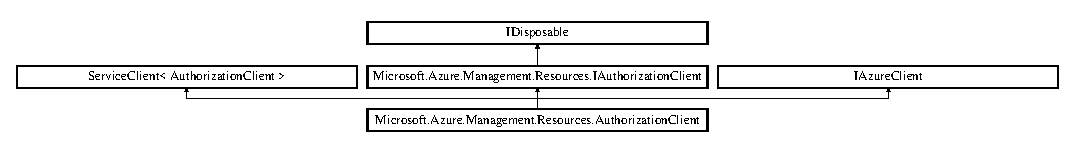
\includegraphics[height=1.538462cm]{class_microsoft_1_1_azure_1_1_management_1_1_resources_1_1_authorization_client}
\end{center}
\end{figure}
\subsection*{Public Member Functions}
\begin{DoxyCompactItemize}
\item 
\hyperlink{class_microsoft_1_1_azure_1_1_management_1_1_resources_1_1_authorization_client_a3715cd8839e758d773915b9b58e24d67}{Authorization\+Client} (Service\+Client\+Credentials credentials, params Delegating\+Handler\mbox{[}$\,$\mbox{]} handlers)
\begin{DoxyCompactList}\small\item\em Initializes a new instance of the \hyperlink{class_microsoft_1_1_azure_1_1_management_1_1_resources_1_1_authorization_client}{Authorization\+Client} class. \end{DoxyCompactList}\item 
\hyperlink{class_microsoft_1_1_azure_1_1_management_1_1_resources_1_1_authorization_client_a04f9939262d07f9be68c0634027a2914}{Authorization\+Client} (Service\+Client\+Credentials credentials, Http\+Client\+Handler root\+Handler, params Delegating\+Handler\mbox{[}$\,$\mbox{]} handlers)
\begin{DoxyCompactList}\small\item\em Initializes a new instance of the \hyperlink{class_microsoft_1_1_azure_1_1_management_1_1_resources_1_1_authorization_client}{Authorization\+Client} class. \end{DoxyCompactList}\item 
\hyperlink{class_microsoft_1_1_azure_1_1_management_1_1_resources_1_1_authorization_client_aa176677b15dcb6fc2e40e891c433643e}{Authorization\+Client} (Uri base\+Uri, Service\+Client\+Credentials credentials, params Delegating\+Handler\mbox{[}$\,$\mbox{]} handlers)
\begin{DoxyCompactList}\small\item\em Initializes a new instance of the \hyperlink{class_microsoft_1_1_azure_1_1_management_1_1_resources_1_1_authorization_client}{Authorization\+Client} class. \end{DoxyCompactList}\item 
\hyperlink{class_microsoft_1_1_azure_1_1_management_1_1_resources_1_1_authorization_client_a32698bd9a5e0310181b435b7a1b7e3f6}{Authorization\+Client} (Uri base\+Uri, Service\+Client\+Credentials credentials, Http\+Client\+Handler root\+Handler, params Delegating\+Handler\mbox{[}$\,$\mbox{]} handlers)
\begin{DoxyCompactList}\small\item\em Initializes a new instance of the \hyperlink{class_microsoft_1_1_azure_1_1_management_1_1_resources_1_1_authorization_client}{Authorization\+Client} class. \end{DoxyCompactList}\end{DoxyCompactItemize}
\subsection*{Protected Member Functions}
\begin{DoxyCompactItemize}
\item 
\hyperlink{class_microsoft_1_1_azure_1_1_management_1_1_resources_1_1_authorization_client_a245003a4655804617e3da30d844ba137}{Authorization\+Client} (params Delegating\+Handler\mbox{[}$\,$\mbox{]} handlers)
\begin{DoxyCompactList}\small\item\em Initializes a new instance of the \hyperlink{class_microsoft_1_1_azure_1_1_management_1_1_resources_1_1_authorization_client}{Authorization\+Client} class. \end{DoxyCompactList}\item 
\hyperlink{class_microsoft_1_1_azure_1_1_management_1_1_resources_1_1_authorization_client_aa01e16fc8851dcb177ca9e4f2d81496b}{Authorization\+Client} (Http\+Client\+Handler root\+Handler, params Delegating\+Handler\mbox{[}$\,$\mbox{]} handlers)
\begin{DoxyCompactList}\small\item\em Initializes a new instance of the \hyperlink{class_microsoft_1_1_azure_1_1_management_1_1_resources_1_1_authorization_client}{Authorization\+Client} class. \end{DoxyCompactList}\item 
\hyperlink{class_microsoft_1_1_azure_1_1_management_1_1_resources_1_1_authorization_client_a1816743585276fc4d6c92cf8c8cefeea}{Authorization\+Client} (Uri base\+Uri, params Delegating\+Handler\mbox{[}$\,$\mbox{]} handlers)
\begin{DoxyCompactList}\small\item\em Initializes a new instance of the \hyperlink{class_microsoft_1_1_azure_1_1_management_1_1_resources_1_1_authorization_client}{Authorization\+Client} class. \end{DoxyCompactList}\item 
\hyperlink{class_microsoft_1_1_azure_1_1_management_1_1_resources_1_1_authorization_client_a4a6c72ff436b176067b909b472651b8d}{Authorization\+Client} (Uri base\+Uri, Http\+Client\+Handler root\+Handler, params Delegating\+Handler\mbox{[}$\,$\mbox{]} handlers)
\begin{DoxyCompactList}\small\item\em Initializes a new instance of the \hyperlink{class_microsoft_1_1_azure_1_1_management_1_1_resources_1_1_authorization_client}{Authorization\+Client} class. \end{DoxyCompactList}\end{DoxyCompactItemize}
\subsection*{Properties}
\begin{DoxyCompactItemize}
\item 
Uri \hyperlink{class_microsoft_1_1_azure_1_1_management_1_1_resources_1_1_authorization_client_a9f0833f17771ecf327c60b8b856ada57}{Base\+Uri}\hspace{0.3cm}{\ttfamily  \mbox{[}get, set\mbox{]}}
\begin{DoxyCompactList}\small\item\em The base U\+RI of the service. \end{DoxyCompactList}\item 
Json\+Serializer\+Settings \hyperlink{class_microsoft_1_1_azure_1_1_management_1_1_resources_1_1_authorization_client_a9ac01a01c4a00c5abf5f6d0b0f701b5d}{Serialization\+Settings}\hspace{0.3cm}{\ttfamily  \mbox{[}get\mbox{]}}
\begin{DoxyCompactList}\small\item\em Gets or sets json serialization settings. \end{DoxyCompactList}\item 
Json\+Serializer\+Settings \hyperlink{class_microsoft_1_1_azure_1_1_management_1_1_resources_1_1_authorization_client_ace10f5afa40a9941ca088971029ad524}{Deserialization\+Settings}\hspace{0.3cm}{\ttfamily  \mbox{[}get\mbox{]}}
\begin{DoxyCompactList}\small\item\em Gets or sets json deserialization settings. \end{DoxyCompactList}\item 
Service\+Client\+Credentials \hyperlink{class_microsoft_1_1_azure_1_1_management_1_1_resources_1_1_authorization_client_ab3e8f6c5773d14a5e823b538b0a611b5}{Credentials}\hspace{0.3cm}{\ttfamily  \mbox{[}get\mbox{]}}
\begin{DoxyCompactList}\small\item\em The management credentials for \hyperlink{namespace_microsoft_1_1_azure}{Azure}. \end{DoxyCompactList}\item 
string \hyperlink{class_microsoft_1_1_azure_1_1_management_1_1_resources_1_1_authorization_client_a6b628c9f7628a01f07ad456c90515aa6}{Subscription\+Id}\hspace{0.3cm}{\ttfamily  \mbox{[}get, set\mbox{]}}
\begin{DoxyCompactList}\small\item\em Gets subscription credentials which uniquely identify \hyperlink{namespace_microsoft}{Microsoft} \hyperlink{namespace_microsoft_1_1_azure}{Azure} subscription. The subscription ID forms part of the U\+RI for every service call. \end{DoxyCompactList}\item 
string \hyperlink{class_microsoft_1_1_azure_1_1_management_1_1_resources_1_1_authorization_client_a626224263775698e6f68e9d50abacaf6}{Api\+Version}\hspace{0.3cm}{\ttfamily  \mbox{[}get\mbox{]}}
\begin{DoxyCompactList}\small\item\em Client Api Version. \end{DoxyCompactList}\item 
string \hyperlink{class_microsoft_1_1_azure_1_1_management_1_1_resources_1_1_authorization_client_a3eb96839bb67595814c900aa438998a4}{Accept\+Language}\hspace{0.3cm}{\ttfamily  \mbox{[}get, set\mbox{]}}
\begin{DoxyCompactList}\small\item\em Gets or sets the preferred language for the response. \end{DoxyCompactList}\item 
int \hyperlink{class_microsoft_1_1_azure_1_1_management_1_1_resources_1_1_authorization_client_ac200a0c2a656262f534e5c9ea35d425b}{Long\+Running\+Operation\+Retry\+Timeout}\hspace{0.3cm}{\ttfamily  \mbox{[}get, set\mbox{]}}
\begin{DoxyCompactList}\small\item\em The retry timeout for Long Running Operations. \end{DoxyCompactList}\item 
virtual \hyperlink{interface_microsoft_1_1_azure_1_1_management_1_1_resources_1_1_i_management_locks_operations}{I\+Management\+Locks\+Operations} {\bfseries Management\+Locks}\hspace{0.3cm}{\ttfamily  \mbox{[}get\mbox{]}}\hypertarget{class_microsoft_1_1_azure_1_1_management_1_1_resources_1_1_authorization_client_aec78e71485f98316623712fbb9a218aa}{}\label{class_microsoft_1_1_azure_1_1_management_1_1_resources_1_1_authorization_client_aec78e71485f98316623712fbb9a218aa}

\end{DoxyCompactItemize}


\subsection{Detailed Description}




\subsection{Constructor \& Destructor Documentation}
\index{Microsoft\+::\+Azure\+::\+Management\+::\+Resources\+::\+Authorization\+Client@{Microsoft\+::\+Azure\+::\+Management\+::\+Resources\+::\+Authorization\+Client}!Authorization\+Client@{Authorization\+Client}}
\index{Authorization\+Client@{Authorization\+Client}!Microsoft\+::\+Azure\+::\+Management\+::\+Resources\+::\+Authorization\+Client@{Microsoft\+::\+Azure\+::\+Management\+::\+Resources\+::\+Authorization\+Client}}
\subsubsection[{\texorpdfstring{Authorization\+Client(params Delegating\+Handler[] handlers)}{AuthorizationClient(params DelegatingHandler[] handlers)}}]{\setlength{\rightskip}{0pt plus 5cm}Microsoft.\+Azure.\+Management.\+Resources.\+Authorization\+Client.\+Authorization\+Client (
\begin{DoxyParamCaption}
\item[{params Delegating\+Handler\mbox{[}$\,$\mbox{]}}]{handlers}
\end{DoxyParamCaption}
)\hspace{0.3cm}{\ttfamily [inline]}, {\ttfamily [protected]}}\hypertarget{class_microsoft_1_1_azure_1_1_management_1_1_resources_1_1_authorization_client_a245003a4655804617e3da30d844ba137}{}\label{class_microsoft_1_1_azure_1_1_management_1_1_resources_1_1_authorization_client_a245003a4655804617e3da30d844ba137}


Initializes a new instance of the \hyperlink{class_microsoft_1_1_azure_1_1_management_1_1_resources_1_1_authorization_client}{Authorization\+Client} class. 


\begin{DoxyParams}{Parameters}
{\em handlers} & Optional. The delegating handlers to add to the http client pipeline. \\
\hline
\end{DoxyParams}
\index{Microsoft\+::\+Azure\+::\+Management\+::\+Resources\+::\+Authorization\+Client@{Microsoft\+::\+Azure\+::\+Management\+::\+Resources\+::\+Authorization\+Client}!Authorization\+Client@{Authorization\+Client}}
\index{Authorization\+Client@{Authorization\+Client}!Microsoft\+::\+Azure\+::\+Management\+::\+Resources\+::\+Authorization\+Client@{Microsoft\+::\+Azure\+::\+Management\+::\+Resources\+::\+Authorization\+Client}}
\subsubsection[{\texorpdfstring{Authorization\+Client(\+Http\+Client\+Handler root\+Handler, params Delegating\+Handler[] handlers)}{AuthorizationClient(HttpClientHandler rootHandler, params DelegatingHandler[] handlers)}}]{\setlength{\rightskip}{0pt plus 5cm}Microsoft.\+Azure.\+Management.\+Resources.\+Authorization\+Client.\+Authorization\+Client (
\begin{DoxyParamCaption}
\item[{Http\+Client\+Handler}]{root\+Handler, }
\item[{params Delegating\+Handler\mbox{[}$\,$\mbox{]}}]{handlers}
\end{DoxyParamCaption}
)\hspace{0.3cm}{\ttfamily [inline]}, {\ttfamily [protected]}}\hypertarget{class_microsoft_1_1_azure_1_1_management_1_1_resources_1_1_authorization_client_aa01e16fc8851dcb177ca9e4f2d81496b}{}\label{class_microsoft_1_1_azure_1_1_management_1_1_resources_1_1_authorization_client_aa01e16fc8851dcb177ca9e4f2d81496b}


Initializes a new instance of the \hyperlink{class_microsoft_1_1_azure_1_1_management_1_1_resources_1_1_authorization_client}{Authorization\+Client} class. 


\begin{DoxyParams}{Parameters}
{\em root\+Handler} & Optional. The http client handler used to handle http transport. \\
\hline
{\em handlers} & Optional. The delegating handlers to add to the http client pipeline. \\
\hline
\end{DoxyParams}
\index{Microsoft\+::\+Azure\+::\+Management\+::\+Resources\+::\+Authorization\+Client@{Microsoft\+::\+Azure\+::\+Management\+::\+Resources\+::\+Authorization\+Client}!Authorization\+Client@{Authorization\+Client}}
\index{Authorization\+Client@{Authorization\+Client}!Microsoft\+::\+Azure\+::\+Management\+::\+Resources\+::\+Authorization\+Client@{Microsoft\+::\+Azure\+::\+Management\+::\+Resources\+::\+Authorization\+Client}}
\subsubsection[{\texorpdfstring{Authorization\+Client(\+Uri base\+Uri, params Delegating\+Handler[] handlers)}{AuthorizationClient(Uri baseUri, params DelegatingHandler[] handlers)}}]{\setlength{\rightskip}{0pt plus 5cm}Microsoft.\+Azure.\+Management.\+Resources.\+Authorization\+Client.\+Authorization\+Client (
\begin{DoxyParamCaption}
\item[{Uri}]{base\+Uri, }
\item[{params Delegating\+Handler\mbox{[}$\,$\mbox{]}}]{handlers}
\end{DoxyParamCaption}
)\hspace{0.3cm}{\ttfamily [inline]}, {\ttfamily [protected]}}\hypertarget{class_microsoft_1_1_azure_1_1_management_1_1_resources_1_1_authorization_client_a1816743585276fc4d6c92cf8c8cefeea}{}\label{class_microsoft_1_1_azure_1_1_management_1_1_resources_1_1_authorization_client_a1816743585276fc4d6c92cf8c8cefeea}


Initializes a new instance of the \hyperlink{class_microsoft_1_1_azure_1_1_management_1_1_resources_1_1_authorization_client}{Authorization\+Client} class. 


\begin{DoxyParams}{Parameters}
{\em base\+Uri} & Optional. The base U\+RI of the service. \\
\hline
{\em handlers} & Optional. The delegating handlers to add to the http client pipeline. \\
\hline
\end{DoxyParams}
\index{Microsoft\+::\+Azure\+::\+Management\+::\+Resources\+::\+Authorization\+Client@{Microsoft\+::\+Azure\+::\+Management\+::\+Resources\+::\+Authorization\+Client}!Authorization\+Client@{Authorization\+Client}}
\index{Authorization\+Client@{Authorization\+Client}!Microsoft\+::\+Azure\+::\+Management\+::\+Resources\+::\+Authorization\+Client@{Microsoft\+::\+Azure\+::\+Management\+::\+Resources\+::\+Authorization\+Client}}
\subsubsection[{\texorpdfstring{Authorization\+Client(\+Uri base\+Uri, Http\+Client\+Handler root\+Handler, params Delegating\+Handler[] handlers)}{AuthorizationClient(Uri baseUri, HttpClientHandler rootHandler, params DelegatingHandler[] handlers)}}]{\setlength{\rightskip}{0pt plus 5cm}Microsoft.\+Azure.\+Management.\+Resources.\+Authorization\+Client.\+Authorization\+Client (
\begin{DoxyParamCaption}
\item[{Uri}]{base\+Uri, }
\item[{Http\+Client\+Handler}]{root\+Handler, }
\item[{params Delegating\+Handler\mbox{[}$\,$\mbox{]}}]{handlers}
\end{DoxyParamCaption}
)\hspace{0.3cm}{\ttfamily [inline]}, {\ttfamily [protected]}}\hypertarget{class_microsoft_1_1_azure_1_1_management_1_1_resources_1_1_authorization_client_a4a6c72ff436b176067b909b472651b8d}{}\label{class_microsoft_1_1_azure_1_1_management_1_1_resources_1_1_authorization_client_a4a6c72ff436b176067b909b472651b8d}


Initializes a new instance of the \hyperlink{class_microsoft_1_1_azure_1_1_management_1_1_resources_1_1_authorization_client}{Authorization\+Client} class. 


\begin{DoxyParams}{Parameters}
{\em base\+Uri} & Optional. The base U\+RI of the service. \\
\hline
{\em root\+Handler} & Optional. The http client handler used to handle http transport. \\
\hline
{\em handlers} & Optional. The delegating handlers to add to the http client pipeline. \\
\hline
\end{DoxyParams}
\index{Microsoft\+::\+Azure\+::\+Management\+::\+Resources\+::\+Authorization\+Client@{Microsoft\+::\+Azure\+::\+Management\+::\+Resources\+::\+Authorization\+Client}!Authorization\+Client@{Authorization\+Client}}
\index{Authorization\+Client@{Authorization\+Client}!Microsoft\+::\+Azure\+::\+Management\+::\+Resources\+::\+Authorization\+Client@{Microsoft\+::\+Azure\+::\+Management\+::\+Resources\+::\+Authorization\+Client}}
\subsubsection[{\texorpdfstring{Authorization\+Client(\+Service\+Client\+Credentials credentials, params Delegating\+Handler[] handlers)}{AuthorizationClient(ServiceClientCredentials credentials, params DelegatingHandler[] handlers)}}]{\setlength{\rightskip}{0pt plus 5cm}Microsoft.\+Azure.\+Management.\+Resources.\+Authorization\+Client.\+Authorization\+Client (
\begin{DoxyParamCaption}
\item[{Service\+Client\+Credentials}]{credentials, }
\item[{params Delegating\+Handler\mbox{[}$\,$\mbox{]}}]{handlers}
\end{DoxyParamCaption}
)\hspace{0.3cm}{\ttfamily [inline]}}\hypertarget{class_microsoft_1_1_azure_1_1_management_1_1_resources_1_1_authorization_client_a3715cd8839e758d773915b9b58e24d67}{}\label{class_microsoft_1_1_azure_1_1_management_1_1_resources_1_1_authorization_client_a3715cd8839e758d773915b9b58e24d67}


Initializes a new instance of the \hyperlink{class_microsoft_1_1_azure_1_1_management_1_1_resources_1_1_authorization_client}{Authorization\+Client} class. 


\begin{DoxyParams}{Parameters}
{\em credentials} & Required. The management credentials for \hyperlink{namespace_microsoft_1_1_azure}{Azure}. \\
\hline
{\em handlers} & Optional. The delegating handlers to add to the http client pipeline. \\
\hline
\end{DoxyParams}
\index{Microsoft\+::\+Azure\+::\+Management\+::\+Resources\+::\+Authorization\+Client@{Microsoft\+::\+Azure\+::\+Management\+::\+Resources\+::\+Authorization\+Client}!Authorization\+Client@{Authorization\+Client}}
\index{Authorization\+Client@{Authorization\+Client}!Microsoft\+::\+Azure\+::\+Management\+::\+Resources\+::\+Authorization\+Client@{Microsoft\+::\+Azure\+::\+Management\+::\+Resources\+::\+Authorization\+Client}}
\subsubsection[{\texorpdfstring{Authorization\+Client(\+Service\+Client\+Credentials credentials, Http\+Client\+Handler root\+Handler, params Delegating\+Handler[] handlers)}{AuthorizationClient(ServiceClientCredentials credentials, HttpClientHandler rootHandler, params DelegatingHandler[] handlers)}}]{\setlength{\rightskip}{0pt plus 5cm}Microsoft.\+Azure.\+Management.\+Resources.\+Authorization\+Client.\+Authorization\+Client (
\begin{DoxyParamCaption}
\item[{Service\+Client\+Credentials}]{credentials, }
\item[{Http\+Client\+Handler}]{root\+Handler, }
\item[{params Delegating\+Handler\mbox{[}$\,$\mbox{]}}]{handlers}
\end{DoxyParamCaption}
)\hspace{0.3cm}{\ttfamily [inline]}}\hypertarget{class_microsoft_1_1_azure_1_1_management_1_1_resources_1_1_authorization_client_a04f9939262d07f9be68c0634027a2914}{}\label{class_microsoft_1_1_azure_1_1_management_1_1_resources_1_1_authorization_client_a04f9939262d07f9be68c0634027a2914}


Initializes a new instance of the \hyperlink{class_microsoft_1_1_azure_1_1_management_1_1_resources_1_1_authorization_client}{Authorization\+Client} class. 


\begin{DoxyParams}{Parameters}
{\em credentials} & Required. The management credentials for \hyperlink{namespace_microsoft_1_1_azure}{Azure}. \\
\hline
{\em root\+Handler} & Optional. The http client handler used to handle http transport. \\
\hline
{\em handlers} & Optional. The delegating handlers to add to the http client pipeline. \\
\hline
\end{DoxyParams}
\index{Microsoft\+::\+Azure\+::\+Management\+::\+Resources\+::\+Authorization\+Client@{Microsoft\+::\+Azure\+::\+Management\+::\+Resources\+::\+Authorization\+Client}!Authorization\+Client@{Authorization\+Client}}
\index{Authorization\+Client@{Authorization\+Client}!Microsoft\+::\+Azure\+::\+Management\+::\+Resources\+::\+Authorization\+Client@{Microsoft\+::\+Azure\+::\+Management\+::\+Resources\+::\+Authorization\+Client}}
\subsubsection[{\texorpdfstring{Authorization\+Client(\+Uri base\+Uri, Service\+Client\+Credentials credentials, params Delegating\+Handler[] handlers)}{AuthorizationClient(Uri baseUri, ServiceClientCredentials credentials, params DelegatingHandler[] handlers)}}]{\setlength{\rightskip}{0pt plus 5cm}Microsoft.\+Azure.\+Management.\+Resources.\+Authorization\+Client.\+Authorization\+Client (
\begin{DoxyParamCaption}
\item[{Uri}]{base\+Uri, }
\item[{Service\+Client\+Credentials}]{credentials, }
\item[{params Delegating\+Handler\mbox{[}$\,$\mbox{]}}]{handlers}
\end{DoxyParamCaption}
)\hspace{0.3cm}{\ttfamily [inline]}}\hypertarget{class_microsoft_1_1_azure_1_1_management_1_1_resources_1_1_authorization_client_aa176677b15dcb6fc2e40e891c433643e}{}\label{class_microsoft_1_1_azure_1_1_management_1_1_resources_1_1_authorization_client_aa176677b15dcb6fc2e40e891c433643e}


Initializes a new instance of the \hyperlink{class_microsoft_1_1_azure_1_1_management_1_1_resources_1_1_authorization_client}{Authorization\+Client} class. 


\begin{DoxyParams}{Parameters}
{\em base\+Uri} & Optional. The base U\+RI of the service. \\
\hline
{\em credentials} & Required. The management credentials for \hyperlink{namespace_microsoft_1_1_azure}{Azure}. \\
\hline
{\em handlers} & Optional. The delegating handlers to add to the http client pipeline. \\
\hline
\end{DoxyParams}
\index{Microsoft\+::\+Azure\+::\+Management\+::\+Resources\+::\+Authorization\+Client@{Microsoft\+::\+Azure\+::\+Management\+::\+Resources\+::\+Authorization\+Client}!Authorization\+Client@{Authorization\+Client}}
\index{Authorization\+Client@{Authorization\+Client}!Microsoft\+::\+Azure\+::\+Management\+::\+Resources\+::\+Authorization\+Client@{Microsoft\+::\+Azure\+::\+Management\+::\+Resources\+::\+Authorization\+Client}}
\subsubsection[{\texorpdfstring{Authorization\+Client(\+Uri base\+Uri, Service\+Client\+Credentials credentials, Http\+Client\+Handler root\+Handler, params Delegating\+Handler[] handlers)}{AuthorizationClient(Uri baseUri, ServiceClientCredentials credentials, HttpClientHandler rootHandler, params DelegatingHandler[] handlers)}}]{\setlength{\rightskip}{0pt plus 5cm}Microsoft.\+Azure.\+Management.\+Resources.\+Authorization\+Client.\+Authorization\+Client (
\begin{DoxyParamCaption}
\item[{Uri}]{base\+Uri, }
\item[{Service\+Client\+Credentials}]{credentials, }
\item[{Http\+Client\+Handler}]{root\+Handler, }
\item[{params Delegating\+Handler\mbox{[}$\,$\mbox{]}}]{handlers}
\end{DoxyParamCaption}
)\hspace{0.3cm}{\ttfamily [inline]}}\hypertarget{class_microsoft_1_1_azure_1_1_management_1_1_resources_1_1_authorization_client_a32698bd9a5e0310181b435b7a1b7e3f6}{}\label{class_microsoft_1_1_azure_1_1_management_1_1_resources_1_1_authorization_client_a32698bd9a5e0310181b435b7a1b7e3f6}


Initializes a new instance of the \hyperlink{class_microsoft_1_1_azure_1_1_management_1_1_resources_1_1_authorization_client}{Authorization\+Client} class. 


\begin{DoxyParams}{Parameters}
{\em base\+Uri} & Optional. The base U\+RI of the service. \\
\hline
{\em credentials} & Required. The management credentials for \hyperlink{namespace_microsoft_1_1_azure}{Azure}. \\
\hline
{\em root\+Handler} & Optional. The http client handler used to handle http transport. \\
\hline
{\em handlers} & Optional. The delegating handlers to add to the http client pipeline. \\
\hline
\end{DoxyParams}


\subsection{Property Documentation}
\index{Microsoft\+::\+Azure\+::\+Management\+::\+Resources\+::\+Authorization\+Client@{Microsoft\+::\+Azure\+::\+Management\+::\+Resources\+::\+Authorization\+Client}!Accept\+Language@{Accept\+Language}}
\index{Accept\+Language@{Accept\+Language}!Microsoft\+::\+Azure\+::\+Management\+::\+Resources\+::\+Authorization\+Client@{Microsoft\+::\+Azure\+::\+Management\+::\+Resources\+::\+Authorization\+Client}}
\subsubsection[{\texorpdfstring{Accept\+Language}{AcceptLanguage}}]{\setlength{\rightskip}{0pt plus 5cm}string Microsoft.\+Azure.\+Management.\+Resources.\+Authorization\+Client.\+Accept\+Language\hspace{0.3cm}{\ttfamily [get]}, {\ttfamily [set]}}\hypertarget{class_microsoft_1_1_azure_1_1_management_1_1_resources_1_1_authorization_client_a3eb96839bb67595814c900aa438998a4}{}\label{class_microsoft_1_1_azure_1_1_management_1_1_resources_1_1_authorization_client_a3eb96839bb67595814c900aa438998a4}


Gets or sets the preferred language for the response. 

\index{Microsoft\+::\+Azure\+::\+Management\+::\+Resources\+::\+Authorization\+Client@{Microsoft\+::\+Azure\+::\+Management\+::\+Resources\+::\+Authorization\+Client}!Api\+Version@{Api\+Version}}
\index{Api\+Version@{Api\+Version}!Microsoft\+::\+Azure\+::\+Management\+::\+Resources\+::\+Authorization\+Client@{Microsoft\+::\+Azure\+::\+Management\+::\+Resources\+::\+Authorization\+Client}}
\subsubsection[{\texorpdfstring{Api\+Version}{ApiVersion}}]{\setlength{\rightskip}{0pt plus 5cm}string Microsoft.\+Azure.\+Management.\+Resources.\+Authorization\+Client.\+Api\+Version\hspace{0.3cm}{\ttfamily [get]}}\hypertarget{class_microsoft_1_1_azure_1_1_management_1_1_resources_1_1_authorization_client_a626224263775698e6f68e9d50abacaf6}{}\label{class_microsoft_1_1_azure_1_1_management_1_1_resources_1_1_authorization_client_a626224263775698e6f68e9d50abacaf6}


Client Api Version. 

\index{Microsoft\+::\+Azure\+::\+Management\+::\+Resources\+::\+Authorization\+Client@{Microsoft\+::\+Azure\+::\+Management\+::\+Resources\+::\+Authorization\+Client}!Base\+Uri@{Base\+Uri}}
\index{Base\+Uri@{Base\+Uri}!Microsoft\+::\+Azure\+::\+Management\+::\+Resources\+::\+Authorization\+Client@{Microsoft\+::\+Azure\+::\+Management\+::\+Resources\+::\+Authorization\+Client}}
\subsubsection[{\texorpdfstring{Base\+Uri}{BaseUri}}]{\setlength{\rightskip}{0pt plus 5cm}Uri Microsoft.\+Azure.\+Management.\+Resources.\+Authorization\+Client.\+Base\+Uri\hspace{0.3cm}{\ttfamily [get]}, {\ttfamily [set]}}\hypertarget{class_microsoft_1_1_azure_1_1_management_1_1_resources_1_1_authorization_client_a9f0833f17771ecf327c60b8b856ada57}{}\label{class_microsoft_1_1_azure_1_1_management_1_1_resources_1_1_authorization_client_a9f0833f17771ecf327c60b8b856ada57}


The base U\+RI of the service. 

\index{Microsoft\+::\+Azure\+::\+Management\+::\+Resources\+::\+Authorization\+Client@{Microsoft\+::\+Azure\+::\+Management\+::\+Resources\+::\+Authorization\+Client}!Credentials@{Credentials}}
\index{Credentials@{Credentials}!Microsoft\+::\+Azure\+::\+Management\+::\+Resources\+::\+Authorization\+Client@{Microsoft\+::\+Azure\+::\+Management\+::\+Resources\+::\+Authorization\+Client}}
\subsubsection[{\texorpdfstring{Credentials}{Credentials}}]{\setlength{\rightskip}{0pt plus 5cm}Service\+Client\+Credentials Microsoft.\+Azure.\+Management.\+Resources.\+Authorization\+Client.\+Credentials\hspace{0.3cm}{\ttfamily [get]}}\hypertarget{class_microsoft_1_1_azure_1_1_management_1_1_resources_1_1_authorization_client_ab3e8f6c5773d14a5e823b538b0a611b5}{}\label{class_microsoft_1_1_azure_1_1_management_1_1_resources_1_1_authorization_client_ab3e8f6c5773d14a5e823b538b0a611b5}


The management credentials for \hyperlink{namespace_microsoft_1_1_azure}{Azure}. 

\index{Microsoft\+::\+Azure\+::\+Management\+::\+Resources\+::\+Authorization\+Client@{Microsoft\+::\+Azure\+::\+Management\+::\+Resources\+::\+Authorization\+Client}!Deserialization\+Settings@{Deserialization\+Settings}}
\index{Deserialization\+Settings@{Deserialization\+Settings}!Microsoft\+::\+Azure\+::\+Management\+::\+Resources\+::\+Authorization\+Client@{Microsoft\+::\+Azure\+::\+Management\+::\+Resources\+::\+Authorization\+Client}}
\subsubsection[{\texorpdfstring{Deserialization\+Settings}{DeserializationSettings}}]{\setlength{\rightskip}{0pt plus 5cm}Json\+Serializer\+Settings Microsoft.\+Azure.\+Management.\+Resources.\+Authorization\+Client.\+Deserialization\+Settings\hspace{0.3cm}{\ttfamily [get]}}\hypertarget{class_microsoft_1_1_azure_1_1_management_1_1_resources_1_1_authorization_client_ace10f5afa40a9941ca088971029ad524}{}\label{class_microsoft_1_1_azure_1_1_management_1_1_resources_1_1_authorization_client_ace10f5afa40a9941ca088971029ad524}


Gets or sets json deserialization settings. 

\index{Microsoft\+::\+Azure\+::\+Management\+::\+Resources\+::\+Authorization\+Client@{Microsoft\+::\+Azure\+::\+Management\+::\+Resources\+::\+Authorization\+Client}!Long\+Running\+Operation\+Retry\+Timeout@{Long\+Running\+Operation\+Retry\+Timeout}}
\index{Long\+Running\+Operation\+Retry\+Timeout@{Long\+Running\+Operation\+Retry\+Timeout}!Microsoft\+::\+Azure\+::\+Management\+::\+Resources\+::\+Authorization\+Client@{Microsoft\+::\+Azure\+::\+Management\+::\+Resources\+::\+Authorization\+Client}}
\subsubsection[{\texorpdfstring{Long\+Running\+Operation\+Retry\+Timeout}{LongRunningOperationRetryTimeout}}]{\setlength{\rightskip}{0pt plus 5cm}int Microsoft.\+Azure.\+Management.\+Resources.\+Authorization\+Client.\+Long\+Running\+Operation\+Retry\+Timeout\hspace{0.3cm}{\ttfamily [get]}, {\ttfamily [set]}}\hypertarget{class_microsoft_1_1_azure_1_1_management_1_1_resources_1_1_authorization_client_ac200a0c2a656262f534e5c9ea35d425b}{}\label{class_microsoft_1_1_azure_1_1_management_1_1_resources_1_1_authorization_client_ac200a0c2a656262f534e5c9ea35d425b}


The retry timeout for Long Running Operations. 

\index{Microsoft\+::\+Azure\+::\+Management\+::\+Resources\+::\+Authorization\+Client@{Microsoft\+::\+Azure\+::\+Management\+::\+Resources\+::\+Authorization\+Client}!Serialization\+Settings@{Serialization\+Settings}}
\index{Serialization\+Settings@{Serialization\+Settings}!Microsoft\+::\+Azure\+::\+Management\+::\+Resources\+::\+Authorization\+Client@{Microsoft\+::\+Azure\+::\+Management\+::\+Resources\+::\+Authorization\+Client}}
\subsubsection[{\texorpdfstring{Serialization\+Settings}{SerializationSettings}}]{\setlength{\rightskip}{0pt plus 5cm}Json\+Serializer\+Settings Microsoft.\+Azure.\+Management.\+Resources.\+Authorization\+Client.\+Serialization\+Settings\hspace{0.3cm}{\ttfamily [get]}}\hypertarget{class_microsoft_1_1_azure_1_1_management_1_1_resources_1_1_authorization_client_a9ac01a01c4a00c5abf5f6d0b0f701b5d}{}\label{class_microsoft_1_1_azure_1_1_management_1_1_resources_1_1_authorization_client_a9ac01a01c4a00c5abf5f6d0b0f701b5d}


Gets or sets json serialization settings. 

\index{Microsoft\+::\+Azure\+::\+Management\+::\+Resources\+::\+Authorization\+Client@{Microsoft\+::\+Azure\+::\+Management\+::\+Resources\+::\+Authorization\+Client}!Subscription\+Id@{Subscription\+Id}}
\index{Subscription\+Id@{Subscription\+Id}!Microsoft\+::\+Azure\+::\+Management\+::\+Resources\+::\+Authorization\+Client@{Microsoft\+::\+Azure\+::\+Management\+::\+Resources\+::\+Authorization\+Client}}
\subsubsection[{\texorpdfstring{Subscription\+Id}{SubscriptionId}}]{\setlength{\rightskip}{0pt plus 5cm}string Microsoft.\+Azure.\+Management.\+Resources.\+Authorization\+Client.\+Subscription\+Id\hspace{0.3cm}{\ttfamily [get]}, {\ttfamily [set]}}\hypertarget{class_microsoft_1_1_azure_1_1_management_1_1_resources_1_1_authorization_client_a6b628c9f7628a01f07ad456c90515aa6}{}\label{class_microsoft_1_1_azure_1_1_management_1_1_resources_1_1_authorization_client_a6b628c9f7628a01f07ad456c90515aa6}


Gets subscription credentials which uniquely identify \hyperlink{namespace_microsoft}{Microsoft} \hyperlink{namespace_microsoft_1_1_azure}{Azure} subscription. The subscription ID forms part of the U\+RI for every service call. 



The documentation for this class was generated from the following file\+:\begin{DoxyCompactItemize}
\item 
files/Authorization\+Client.\+cs\end{DoxyCompactItemize}

\hypertarget{class_microsoft_1_1_azure_1_1_management_1_1_resources_1_1_feature_client}{}\section{Microsoft.\+Azure.\+Management.\+Resources.\+Feature\+Client Class Reference}
\label{class_microsoft_1_1_azure_1_1_management_1_1_resources_1_1_feature_client}\index{Microsoft.\+Azure.\+Management.\+Resources.\+Feature\+Client@{Microsoft.\+Azure.\+Management.\+Resources.\+Feature\+Client}}


 


Inheritance diagram for Microsoft.\+Azure.\+Management.\+Resources.\+Feature\+Client\+:\begin{figure}[H]
\begin{center}
\leavevmode
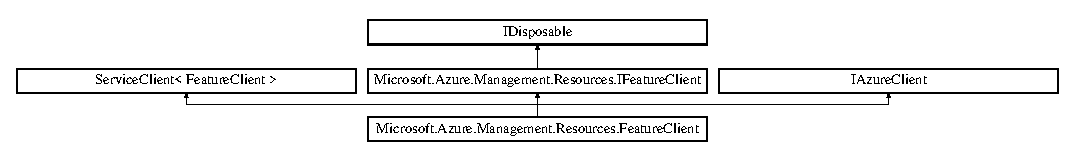
\includegraphics[height=1.676647cm]{class_microsoft_1_1_azure_1_1_management_1_1_resources_1_1_feature_client}
\end{center}
\end{figure}
\subsection*{Public Member Functions}
\begin{DoxyCompactItemize}
\item 
\hyperlink{class_microsoft_1_1_azure_1_1_management_1_1_resources_1_1_feature_client_a42702546153fd199d8e0d872900f53ea}{Feature\+Client} (Service\+Client\+Credentials credentials, params Delegating\+Handler\mbox{[}$\,$\mbox{]} handlers)
\begin{DoxyCompactList}\small\item\em Initializes a new instance of the \hyperlink{class_microsoft_1_1_azure_1_1_management_1_1_resources_1_1_feature_client}{Feature\+Client} class. \end{DoxyCompactList}\item 
\hyperlink{class_microsoft_1_1_azure_1_1_management_1_1_resources_1_1_feature_client_a9e2c0febf863ca5ecaaa3b456b90aea8}{Feature\+Client} (Service\+Client\+Credentials credentials, Http\+Client\+Handler root\+Handler, params Delegating\+Handler\mbox{[}$\,$\mbox{]} handlers)
\begin{DoxyCompactList}\small\item\em Initializes a new instance of the \hyperlink{class_microsoft_1_1_azure_1_1_management_1_1_resources_1_1_feature_client}{Feature\+Client} class. \end{DoxyCompactList}\item 
\hyperlink{class_microsoft_1_1_azure_1_1_management_1_1_resources_1_1_feature_client_a49828cd8b5c2c87d5ead7916d86ae850}{Feature\+Client} (Uri base\+Uri, Service\+Client\+Credentials credentials, params Delegating\+Handler\mbox{[}$\,$\mbox{]} handlers)
\begin{DoxyCompactList}\small\item\em Initializes a new instance of the \hyperlink{class_microsoft_1_1_azure_1_1_management_1_1_resources_1_1_feature_client}{Feature\+Client} class. \end{DoxyCompactList}\item 
\hyperlink{class_microsoft_1_1_azure_1_1_management_1_1_resources_1_1_feature_client_a5d277cb1b740af70ab807a1cc53cfb17}{Feature\+Client} (Uri base\+Uri, Service\+Client\+Credentials credentials, Http\+Client\+Handler root\+Handler, params Delegating\+Handler\mbox{[}$\,$\mbox{]} handlers)
\begin{DoxyCompactList}\small\item\em Initializes a new instance of the \hyperlink{class_microsoft_1_1_azure_1_1_management_1_1_resources_1_1_feature_client}{Feature\+Client} class. \end{DoxyCompactList}\end{DoxyCompactItemize}
\subsection*{Protected Member Functions}
\begin{DoxyCompactItemize}
\item 
\hyperlink{class_microsoft_1_1_azure_1_1_management_1_1_resources_1_1_feature_client_af2f4eef7afd7d5438667d2599e8d3b29}{Feature\+Client} (params Delegating\+Handler\mbox{[}$\,$\mbox{]} handlers)
\begin{DoxyCompactList}\small\item\em Initializes a new instance of the \hyperlink{class_microsoft_1_1_azure_1_1_management_1_1_resources_1_1_feature_client}{Feature\+Client} class. \end{DoxyCompactList}\item 
\hyperlink{class_microsoft_1_1_azure_1_1_management_1_1_resources_1_1_feature_client_a8ba9130cd506de9958e4b9a152b70bdf}{Feature\+Client} (Http\+Client\+Handler root\+Handler, params Delegating\+Handler\mbox{[}$\,$\mbox{]} handlers)
\begin{DoxyCompactList}\small\item\em Initializes a new instance of the \hyperlink{class_microsoft_1_1_azure_1_1_management_1_1_resources_1_1_feature_client}{Feature\+Client} class. \end{DoxyCompactList}\item 
\hyperlink{class_microsoft_1_1_azure_1_1_management_1_1_resources_1_1_feature_client_a37ed3dbc886e58fd67c69304e5479b83}{Feature\+Client} (Uri base\+Uri, params Delegating\+Handler\mbox{[}$\,$\mbox{]} handlers)
\begin{DoxyCompactList}\small\item\em Initializes a new instance of the \hyperlink{class_microsoft_1_1_azure_1_1_management_1_1_resources_1_1_feature_client}{Feature\+Client} class. \end{DoxyCompactList}\item 
\hyperlink{class_microsoft_1_1_azure_1_1_management_1_1_resources_1_1_feature_client_a969baf3e5fe72b5287eddc4ba8d7bcf9}{Feature\+Client} (Uri base\+Uri, Http\+Client\+Handler root\+Handler, params Delegating\+Handler\mbox{[}$\,$\mbox{]} handlers)
\begin{DoxyCompactList}\small\item\em Initializes a new instance of the \hyperlink{class_microsoft_1_1_azure_1_1_management_1_1_resources_1_1_feature_client}{Feature\+Client} class. \end{DoxyCompactList}\end{DoxyCompactItemize}
\subsection*{Properties}
\begin{DoxyCompactItemize}
\item 
Uri \hyperlink{class_microsoft_1_1_azure_1_1_management_1_1_resources_1_1_feature_client_afada16c589e422353970ff4a284e9d27}{Base\+Uri}\hspace{0.3cm}{\ttfamily  \mbox{[}get, set\mbox{]}}
\begin{DoxyCompactList}\small\item\em The base U\+RI of the service. \end{DoxyCompactList}\item 
Json\+Serializer\+Settings \hyperlink{class_microsoft_1_1_azure_1_1_management_1_1_resources_1_1_feature_client_a979dfa652c2df74dc167dc45ebe35e21}{Serialization\+Settings}\hspace{0.3cm}{\ttfamily  \mbox{[}get\mbox{]}}
\begin{DoxyCompactList}\small\item\em Gets or sets json serialization settings. \end{DoxyCompactList}\item 
Json\+Serializer\+Settings \hyperlink{class_microsoft_1_1_azure_1_1_management_1_1_resources_1_1_feature_client_a10adf4626692877ba4e344289b9a64e8}{Deserialization\+Settings}\hspace{0.3cm}{\ttfamily  \mbox{[}get\mbox{]}}
\begin{DoxyCompactList}\small\item\em Gets or sets json deserialization settings. \end{DoxyCompactList}\item 
Service\+Client\+Credentials \hyperlink{class_microsoft_1_1_azure_1_1_management_1_1_resources_1_1_feature_client_a8479d66ee91c999f198ef7f2a5cbaac5}{Credentials}\hspace{0.3cm}{\ttfamily  \mbox{[}get\mbox{]}}
\begin{DoxyCompactList}\small\item\em The management credentials for \hyperlink{namespace_microsoft_1_1_azure}{Azure}. \end{DoxyCompactList}\item 
string \hyperlink{class_microsoft_1_1_azure_1_1_management_1_1_resources_1_1_feature_client_a813f243553200ffdf6a8c6fd77196a8c}{Subscription\+Id}\hspace{0.3cm}{\ttfamily  \mbox{[}get, set\mbox{]}}
\begin{DoxyCompactList}\small\item\em Gets subscription credentials which uniquely identify \hyperlink{namespace_microsoft}{Microsoft} \hyperlink{namespace_microsoft_1_1_azure}{Azure} subscription. The subscription ID forms part of the U\+RI for every service call. \end{DoxyCompactList}\item 
string \hyperlink{class_microsoft_1_1_azure_1_1_management_1_1_resources_1_1_feature_client_ab9ec640be2a72809c8d0fbf59f9601e9}{Api\+Version}\hspace{0.3cm}{\ttfamily  \mbox{[}get\mbox{]}}
\begin{DoxyCompactList}\small\item\em Client Api Version. \end{DoxyCompactList}\item 
string \hyperlink{class_microsoft_1_1_azure_1_1_management_1_1_resources_1_1_feature_client_a12c737e4db1139025734fddc6e609dbd}{Accept\+Language}\hspace{0.3cm}{\ttfamily  \mbox{[}get, set\mbox{]}}
\begin{DoxyCompactList}\small\item\em Gets or sets the preferred language for the response. \end{DoxyCompactList}\item 
int \hyperlink{class_microsoft_1_1_azure_1_1_management_1_1_resources_1_1_feature_client_ad5ff8d180c179578f08ed658d4134d56}{Long\+Running\+Operation\+Retry\+Timeout}\hspace{0.3cm}{\ttfamily  \mbox{[}get, set\mbox{]}}
\begin{DoxyCompactList}\small\item\em The retry timeout for Long Running Operations. \end{DoxyCompactList}\item 
virtual \hyperlink{interface_microsoft_1_1_azure_1_1_management_1_1_resources_1_1_i_features_operations}{I\+Features\+Operations} {\bfseries Features}\hspace{0.3cm}{\ttfamily  \mbox{[}get\mbox{]}}\hypertarget{class_microsoft_1_1_azure_1_1_management_1_1_resources_1_1_feature_client_a0ab16e5e5a7bdd0cd0ab0b16999d26e0}{}\label{class_microsoft_1_1_azure_1_1_management_1_1_resources_1_1_feature_client_a0ab16e5e5a7bdd0cd0ab0b16999d26e0}

\end{DoxyCompactItemize}


\subsection{Detailed Description}




\subsection{Constructor \& Destructor Documentation}
\index{Microsoft\+::\+Azure\+::\+Management\+::\+Resources\+::\+Feature\+Client@{Microsoft\+::\+Azure\+::\+Management\+::\+Resources\+::\+Feature\+Client}!Feature\+Client@{Feature\+Client}}
\index{Feature\+Client@{Feature\+Client}!Microsoft\+::\+Azure\+::\+Management\+::\+Resources\+::\+Feature\+Client@{Microsoft\+::\+Azure\+::\+Management\+::\+Resources\+::\+Feature\+Client}}
\subsubsection[{\texorpdfstring{Feature\+Client(params Delegating\+Handler[] handlers)}{FeatureClient(params DelegatingHandler[] handlers)}}]{\setlength{\rightskip}{0pt plus 5cm}Microsoft.\+Azure.\+Management.\+Resources.\+Feature\+Client.\+Feature\+Client (
\begin{DoxyParamCaption}
\item[{params Delegating\+Handler\mbox{[}$\,$\mbox{]}}]{handlers}
\end{DoxyParamCaption}
)\hspace{0.3cm}{\ttfamily [inline]}, {\ttfamily [protected]}}\hypertarget{class_microsoft_1_1_azure_1_1_management_1_1_resources_1_1_feature_client_af2f4eef7afd7d5438667d2599e8d3b29}{}\label{class_microsoft_1_1_azure_1_1_management_1_1_resources_1_1_feature_client_af2f4eef7afd7d5438667d2599e8d3b29}


Initializes a new instance of the \hyperlink{class_microsoft_1_1_azure_1_1_management_1_1_resources_1_1_feature_client}{Feature\+Client} class. 


\begin{DoxyParams}{Parameters}
{\em handlers} & Optional. The delegating handlers to add to the http client pipeline. \\
\hline
\end{DoxyParams}
\index{Microsoft\+::\+Azure\+::\+Management\+::\+Resources\+::\+Feature\+Client@{Microsoft\+::\+Azure\+::\+Management\+::\+Resources\+::\+Feature\+Client}!Feature\+Client@{Feature\+Client}}
\index{Feature\+Client@{Feature\+Client}!Microsoft\+::\+Azure\+::\+Management\+::\+Resources\+::\+Feature\+Client@{Microsoft\+::\+Azure\+::\+Management\+::\+Resources\+::\+Feature\+Client}}
\subsubsection[{\texorpdfstring{Feature\+Client(\+Http\+Client\+Handler root\+Handler, params Delegating\+Handler[] handlers)}{FeatureClient(HttpClientHandler rootHandler, params DelegatingHandler[] handlers)}}]{\setlength{\rightskip}{0pt plus 5cm}Microsoft.\+Azure.\+Management.\+Resources.\+Feature\+Client.\+Feature\+Client (
\begin{DoxyParamCaption}
\item[{Http\+Client\+Handler}]{root\+Handler, }
\item[{params Delegating\+Handler\mbox{[}$\,$\mbox{]}}]{handlers}
\end{DoxyParamCaption}
)\hspace{0.3cm}{\ttfamily [inline]}, {\ttfamily [protected]}}\hypertarget{class_microsoft_1_1_azure_1_1_management_1_1_resources_1_1_feature_client_a8ba9130cd506de9958e4b9a152b70bdf}{}\label{class_microsoft_1_1_azure_1_1_management_1_1_resources_1_1_feature_client_a8ba9130cd506de9958e4b9a152b70bdf}


Initializes a new instance of the \hyperlink{class_microsoft_1_1_azure_1_1_management_1_1_resources_1_1_feature_client}{Feature\+Client} class. 


\begin{DoxyParams}{Parameters}
{\em root\+Handler} & Optional. The http client handler used to handle http transport. \\
\hline
{\em handlers} & Optional. The delegating handlers to add to the http client pipeline. \\
\hline
\end{DoxyParams}
\index{Microsoft\+::\+Azure\+::\+Management\+::\+Resources\+::\+Feature\+Client@{Microsoft\+::\+Azure\+::\+Management\+::\+Resources\+::\+Feature\+Client}!Feature\+Client@{Feature\+Client}}
\index{Feature\+Client@{Feature\+Client}!Microsoft\+::\+Azure\+::\+Management\+::\+Resources\+::\+Feature\+Client@{Microsoft\+::\+Azure\+::\+Management\+::\+Resources\+::\+Feature\+Client}}
\subsubsection[{\texorpdfstring{Feature\+Client(\+Uri base\+Uri, params Delegating\+Handler[] handlers)}{FeatureClient(Uri baseUri, params DelegatingHandler[] handlers)}}]{\setlength{\rightskip}{0pt plus 5cm}Microsoft.\+Azure.\+Management.\+Resources.\+Feature\+Client.\+Feature\+Client (
\begin{DoxyParamCaption}
\item[{Uri}]{base\+Uri, }
\item[{params Delegating\+Handler\mbox{[}$\,$\mbox{]}}]{handlers}
\end{DoxyParamCaption}
)\hspace{0.3cm}{\ttfamily [inline]}, {\ttfamily [protected]}}\hypertarget{class_microsoft_1_1_azure_1_1_management_1_1_resources_1_1_feature_client_a37ed3dbc886e58fd67c69304e5479b83}{}\label{class_microsoft_1_1_azure_1_1_management_1_1_resources_1_1_feature_client_a37ed3dbc886e58fd67c69304e5479b83}


Initializes a new instance of the \hyperlink{class_microsoft_1_1_azure_1_1_management_1_1_resources_1_1_feature_client}{Feature\+Client} class. 


\begin{DoxyParams}{Parameters}
{\em base\+Uri} & Optional. The base U\+RI of the service. \\
\hline
{\em handlers} & Optional. The delegating handlers to add to the http client pipeline. \\
\hline
\end{DoxyParams}
\index{Microsoft\+::\+Azure\+::\+Management\+::\+Resources\+::\+Feature\+Client@{Microsoft\+::\+Azure\+::\+Management\+::\+Resources\+::\+Feature\+Client}!Feature\+Client@{Feature\+Client}}
\index{Feature\+Client@{Feature\+Client}!Microsoft\+::\+Azure\+::\+Management\+::\+Resources\+::\+Feature\+Client@{Microsoft\+::\+Azure\+::\+Management\+::\+Resources\+::\+Feature\+Client}}
\subsubsection[{\texorpdfstring{Feature\+Client(\+Uri base\+Uri, Http\+Client\+Handler root\+Handler, params Delegating\+Handler[] handlers)}{FeatureClient(Uri baseUri, HttpClientHandler rootHandler, params DelegatingHandler[] handlers)}}]{\setlength{\rightskip}{0pt plus 5cm}Microsoft.\+Azure.\+Management.\+Resources.\+Feature\+Client.\+Feature\+Client (
\begin{DoxyParamCaption}
\item[{Uri}]{base\+Uri, }
\item[{Http\+Client\+Handler}]{root\+Handler, }
\item[{params Delegating\+Handler\mbox{[}$\,$\mbox{]}}]{handlers}
\end{DoxyParamCaption}
)\hspace{0.3cm}{\ttfamily [inline]}, {\ttfamily [protected]}}\hypertarget{class_microsoft_1_1_azure_1_1_management_1_1_resources_1_1_feature_client_a969baf3e5fe72b5287eddc4ba8d7bcf9}{}\label{class_microsoft_1_1_azure_1_1_management_1_1_resources_1_1_feature_client_a969baf3e5fe72b5287eddc4ba8d7bcf9}


Initializes a new instance of the \hyperlink{class_microsoft_1_1_azure_1_1_management_1_1_resources_1_1_feature_client}{Feature\+Client} class. 


\begin{DoxyParams}{Parameters}
{\em base\+Uri} & Optional. The base U\+RI of the service. \\
\hline
{\em root\+Handler} & Optional. The http client handler used to handle http transport. \\
\hline
{\em handlers} & Optional. The delegating handlers to add to the http client pipeline. \\
\hline
\end{DoxyParams}
\index{Microsoft\+::\+Azure\+::\+Management\+::\+Resources\+::\+Feature\+Client@{Microsoft\+::\+Azure\+::\+Management\+::\+Resources\+::\+Feature\+Client}!Feature\+Client@{Feature\+Client}}
\index{Feature\+Client@{Feature\+Client}!Microsoft\+::\+Azure\+::\+Management\+::\+Resources\+::\+Feature\+Client@{Microsoft\+::\+Azure\+::\+Management\+::\+Resources\+::\+Feature\+Client}}
\subsubsection[{\texorpdfstring{Feature\+Client(\+Service\+Client\+Credentials credentials, params Delegating\+Handler[] handlers)}{FeatureClient(ServiceClientCredentials credentials, params DelegatingHandler[] handlers)}}]{\setlength{\rightskip}{0pt plus 5cm}Microsoft.\+Azure.\+Management.\+Resources.\+Feature\+Client.\+Feature\+Client (
\begin{DoxyParamCaption}
\item[{Service\+Client\+Credentials}]{credentials, }
\item[{params Delegating\+Handler\mbox{[}$\,$\mbox{]}}]{handlers}
\end{DoxyParamCaption}
)\hspace{0.3cm}{\ttfamily [inline]}}\hypertarget{class_microsoft_1_1_azure_1_1_management_1_1_resources_1_1_feature_client_a42702546153fd199d8e0d872900f53ea}{}\label{class_microsoft_1_1_azure_1_1_management_1_1_resources_1_1_feature_client_a42702546153fd199d8e0d872900f53ea}


Initializes a new instance of the \hyperlink{class_microsoft_1_1_azure_1_1_management_1_1_resources_1_1_feature_client}{Feature\+Client} class. 


\begin{DoxyParams}{Parameters}
{\em credentials} & Required. The management credentials for \hyperlink{namespace_microsoft_1_1_azure}{Azure}. \\
\hline
{\em handlers} & Optional. The delegating handlers to add to the http client pipeline. \\
\hline
\end{DoxyParams}
\index{Microsoft\+::\+Azure\+::\+Management\+::\+Resources\+::\+Feature\+Client@{Microsoft\+::\+Azure\+::\+Management\+::\+Resources\+::\+Feature\+Client}!Feature\+Client@{Feature\+Client}}
\index{Feature\+Client@{Feature\+Client}!Microsoft\+::\+Azure\+::\+Management\+::\+Resources\+::\+Feature\+Client@{Microsoft\+::\+Azure\+::\+Management\+::\+Resources\+::\+Feature\+Client}}
\subsubsection[{\texorpdfstring{Feature\+Client(\+Service\+Client\+Credentials credentials, Http\+Client\+Handler root\+Handler, params Delegating\+Handler[] handlers)}{FeatureClient(ServiceClientCredentials credentials, HttpClientHandler rootHandler, params DelegatingHandler[] handlers)}}]{\setlength{\rightskip}{0pt plus 5cm}Microsoft.\+Azure.\+Management.\+Resources.\+Feature\+Client.\+Feature\+Client (
\begin{DoxyParamCaption}
\item[{Service\+Client\+Credentials}]{credentials, }
\item[{Http\+Client\+Handler}]{root\+Handler, }
\item[{params Delegating\+Handler\mbox{[}$\,$\mbox{]}}]{handlers}
\end{DoxyParamCaption}
)\hspace{0.3cm}{\ttfamily [inline]}}\hypertarget{class_microsoft_1_1_azure_1_1_management_1_1_resources_1_1_feature_client_a9e2c0febf863ca5ecaaa3b456b90aea8}{}\label{class_microsoft_1_1_azure_1_1_management_1_1_resources_1_1_feature_client_a9e2c0febf863ca5ecaaa3b456b90aea8}


Initializes a new instance of the \hyperlink{class_microsoft_1_1_azure_1_1_management_1_1_resources_1_1_feature_client}{Feature\+Client} class. 


\begin{DoxyParams}{Parameters}
{\em credentials} & Required. The management credentials for \hyperlink{namespace_microsoft_1_1_azure}{Azure}. \\
\hline
{\em root\+Handler} & Optional. The http client handler used to handle http transport. \\
\hline
{\em handlers} & Optional. The delegating handlers to add to the http client pipeline. \\
\hline
\end{DoxyParams}
\index{Microsoft\+::\+Azure\+::\+Management\+::\+Resources\+::\+Feature\+Client@{Microsoft\+::\+Azure\+::\+Management\+::\+Resources\+::\+Feature\+Client}!Feature\+Client@{Feature\+Client}}
\index{Feature\+Client@{Feature\+Client}!Microsoft\+::\+Azure\+::\+Management\+::\+Resources\+::\+Feature\+Client@{Microsoft\+::\+Azure\+::\+Management\+::\+Resources\+::\+Feature\+Client}}
\subsubsection[{\texorpdfstring{Feature\+Client(\+Uri base\+Uri, Service\+Client\+Credentials credentials, params Delegating\+Handler[] handlers)}{FeatureClient(Uri baseUri, ServiceClientCredentials credentials, params DelegatingHandler[] handlers)}}]{\setlength{\rightskip}{0pt plus 5cm}Microsoft.\+Azure.\+Management.\+Resources.\+Feature\+Client.\+Feature\+Client (
\begin{DoxyParamCaption}
\item[{Uri}]{base\+Uri, }
\item[{Service\+Client\+Credentials}]{credentials, }
\item[{params Delegating\+Handler\mbox{[}$\,$\mbox{]}}]{handlers}
\end{DoxyParamCaption}
)\hspace{0.3cm}{\ttfamily [inline]}}\hypertarget{class_microsoft_1_1_azure_1_1_management_1_1_resources_1_1_feature_client_a49828cd8b5c2c87d5ead7916d86ae850}{}\label{class_microsoft_1_1_azure_1_1_management_1_1_resources_1_1_feature_client_a49828cd8b5c2c87d5ead7916d86ae850}


Initializes a new instance of the \hyperlink{class_microsoft_1_1_azure_1_1_management_1_1_resources_1_1_feature_client}{Feature\+Client} class. 


\begin{DoxyParams}{Parameters}
{\em base\+Uri} & Optional. The base U\+RI of the service. \\
\hline
{\em credentials} & Required. The management credentials for \hyperlink{namespace_microsoft_1_1_azure}{Azure}. \\
\hline
{\em handlers} & Optional. The delegating handlers to add to the http client pipeline. \\
\hline
\end{DoxyParams}
\index{Microsoft\+::\+Azure\+::\+Management\+::\+Resources\+::\+Feature\+Client@{Microsoft\+::\+Azure\+::\+Management\+::\+Resources\+::\+Feature\+Client}!Feature\+Client@{Feature\+Client}}
\index{Feature\+Client@{Feature\+Client}!Microsoft\+::\+Azure\+::\+Management\+::\+Resources\+::\+Feature\+Client@{Microsoft\+::\+Azure\+::\+Management\+::\+Resources\+::\+Feature\+Client}}
\subsubsection[{\texorpdfstring{Feature\+Client(\+Uri base\+Uri, Service\+Client\+Credentials credentials, Http\+Client\+Handler root\+Handler, params Delegating\+Handler[] handlers)}{FeatureClient(Uri baseUri, ServiceClientCredentials credentials, HttpClientHandler rootHandler, params DelegatingHandler[] handlers)}}]{\setlength{\rightskip}{0pt plus 5cm}Microsoft.\+Azure.\+Management.\+Resources.\+Feature\+Client.\+Feature\+Client (
\begin{DoxyParamCaption}
\item[{Uri}]{base\+Uri, }
\item[{Service\+Client\+Credentials}]{credentials, }
\item[{Http\+Client\+Handler}]{root\+Handler, }
\item[{params Delegating\+Handler\mbox{[}$\,$\mbox{]}}]{handlers}
\end{DoxyParamCaption}
)\hspace{0.3cm}{\ttfamily [inline]}}\hypertarget{class_microsoft_1_1_azure_1_1_management_1_1_resources_1_1_feature_client_a5d277cb1b740af70ab807a1cc53cfb17}{}\label{class_microsoft_1_1_azure_1_1_management_1_1_resources_1_1_feature_client_a5d277cb1b740af70ab807a1cc53cfb17}


Initializes a new instance of the \hyperlink{class_microsoft_1_1_azure_1_1_management_1_1_resources_1_1_feature_client}{Feature\+Client} class. 


\begin{DoxyParams}{Parameters}
{\em base\+Uri} & Optional. The base U\+RI of the service. \\
\hline
{\em credentials} & Required. The management credentials for \hyperlink{namespace_microsoft_1_1_azure}{Azure}. \\
\hline
{\em root\+Handler} & Optional. The http client handler used to handle http transport. \\
\hline
{\em handlers} & Optional. The delegating handlers to add to the http client pipeline. \\
\hline
\end{DoxyParams}


\subsection{Property Documentation}
\index{Microsoft\+::\+Azure\+::\+Management\+::\+Resources\+::\+Feature\+Client@{Microsoft\+::\+Azure\+::\+Management\+::\+Resources\+::\+Feature\+Client}!Accept\+Language@{Accept\+Language}}
\index{Accept\+Language@{Accept\+Language}!Microsoft\+::\+Azure\+::\+Management\+::\+Resources\+::\+Feature\+Client@{Microsoft\+::\+Azure\+::\+Management\+::\+Resources\+::\+Feature\+Client}}
\subsubsection[{\texorpdfstring{Accept\+Language}{AcceptLanguage}}]{\setlength{\rightskip}{0pt plus 5cm}string Microsoft.\+Azure.\+Management.\+Resources.\+Feature\+Client.\+Accept\+Language\hspace{0.3cm}{\ttfamily [get]}, {\ttfamily [set]}}\hypertarget{class_microsoft_1_1_azure_1_1_management_1_1_resources_1_1_feature_client_a12c737e4db1139025734fddc6e609dbd}{}\label{class_microsoft_1_1_azure_1_1_management_1_1_resources_1_1_feature_client_a12c737e4db1139025734fddc6e609dbd}


Gets or sets the preferred language for the response. 

\index{Microsoft\+::\+Azure\+::\+Management\+::\+Resources\+::\+Feature\+Client@{Microsoft\+::\+Azure\+::\+Management\+::\+Resources\+::\+Feature\+Client}!Api\+Version@{Api\+Version}}
\index{Api\+Version@{Api\+Version}!Microsoft\+::\+Azure\+::\+Management\+::\+Resources\+::\+Feature\+Client@{Microsoft\+::\+Azure\+::\+Management\+::\+Resources\+::\+Feature\+Client}}
\subsubsection[{\texorpdfstring{Api\+Version}{ApiVersion}}]{\setlength{\rightskip}{0pt plus 5cm}string Microsoft.\+Azure.\+Management.\+Resources.\+Feature\+Client.\+Api\+Version\hspace{0.3cm}{\ttfamily [get]}}\hypertarget{class_microsoft_1_1_azure_1_1_management_1_1_resources_1_1_feature_client_ab9ec640be2a72809c8d0fbf59f9601e9}{}\label{class_microsoft_1_1_azure_1_1_management_1_1_resources_1_1_feature_client_ab9ec640be2a72809c8d0fbf59f9601e9}


Client Api Version. 

\index{Microsoft\+::\+Azure\+::\+Management\+::\+Resources\+::\+Feature\+Client@{Microsoft\+::\+Azure\+::\+Management\+::\+Resources\+::\+Feature\+Client}!Base\+Uri@{Base\+Uri}}
\index{Base\+Uri@{Base\+Uri}!Microsoft\+::\+Azure\+::\+Management\+::\+Resources\+::\+Feature\+Client@{Microsoft\+::\+Azure\+::\+Management\+::\+Resources\+::\+Feature\+Client}}
\subsubsection[{\texorpdfstring{Base\+Uri}{BaseUri}}]{\setlength{\rightskip}{0pt plus 5cm}Uri Microsoft.\+Azure.\+Management.\+Resources.\+Feature\+Client.\+Base\+Uri\hspace{0.3cm}{\ttfamily [get]}, {\ttfamily [set]}}\hypertarget{class_microsoft_1_1_azure_1_1_management_1_1_resources_1_1_feature_client_afada16c589e422353970ff4a284e9d27}{}\label{class_microsoft_1_1_azure_1_1_management_1_1_resources_1_1_feature_client_afada16c589e422353970ff4a284e9d27}


The base U\+RI of the service. 

\index{Microsoft\+::\+Azure\+::\+Management\+::\+Resources\+::\+Feature\+Client@{Microsoft\+::\+Azure\+::\+Management\+::\+Resources\+::\+Feature\+Client}!Credentials@{Credentials}}
\index{Credentials@{Credentials}!Microsoft\+::\+Azure\+::\+Management\+::\+Resources\+::\+Feature\+Client@{Microsoft\+::\+Azure\+::\+Management\+::\+Resources\+::\+Feature\+Client}}
\subsubsection[{\texorpdfstring{Credentials}{Credentials}}]{\setlength{\rightskip}{0pt plus 5cm}Service\+Client\+Credentials Microsoft.\+Azure.\+Management.\+Resources.\+Feature\+Client.\+Credentials\hspace{0.3cm}{\ttfamily [get]}}\hypertarget{class_microsoft_1_1_azure_1_1_management_1_1_resources_1_1_feature_client_a8479d66ee91c999f198ef7f2a5cbaac5}{}\label{class_microsoft_1_1_azure_1_1_management_1_1_resources_1_1_feature_client_a8479d66ee91c999f198ef7f2a5cbaac5}


The management credentials for \hyperlink{namespace_microsoft_1_1_azure}{Azure}. 

\index{Microsoft\+::\+Azure\+::\+Management\+::\+Resources\+::\+Feature\+Client@{Microsoft\+::\+Azure\+::\+Management\+::\+Resources\+::\+Feature\+Client}!Deserialization\+Settings@{Deserialization\+Settings}}
\index{Deserialization\+Settings@{Deserialization\+Settings}!Microsoft\+::\+Azure\+::\+Management\+::\+Resources\+::\+Feature\+Client@{Microsoft\+::\+Azure\+::\+Management\+::\+Resources\+::\+Feature\+Client}}
\subsubsection[{\texorpdfstring{Deserialization\+Settings}{DeserializationSettings}}]{\setlength{\rightskip}{0pt plus 5cm}Json\+Serializer\+Settings Microsoft.\+Azure.\+Management.\+Resources.\+Feature\+Client.\+Deserialization\+Settings\hspace{0.3cm}{\ttfamily [get]}}\hypertarget{class_microsoft_1_1_azure_1_1_management_1_1_resources_1_1_feature_client_a10adf4626692877ba4e344289b9a64e8}{}\label{class_microsoft_1_1_azure_1_1_management_1_1_resources_1_1_feature_client_a10adf4626692877ba4e344289b9a64e8}


Gets or sets json deserialization settings. 

\index{Microsoft\+::\+Azure\+::\+Management\+::\+Resources\+::\+Feature\+Client@{Microsoft\+::\+Azure\+::\+Management\+::\+Resources\+::\+Feature\+Client}!Long\+Running\+Operation\+Retry\+Timeout@{Long\+Running\+Operation\+Retry\+Timeout}}
\index{Long\+Running\+Operation\+Retry\+Timeout@{Long\+Running\+Operation\+Retry\+Timeout}!Microsoft\+::\+Azure\+::\+Management\+::\+Resources\+::\+Feature\+Client@{Microsoft\+::\+Azure\+::\+Management\+::\+Resources\+::\+Feature\+Client}}
\subsubsection[{\texorpdfstring{Long\+Running\+Operation\+Retry\+Timeout}{LongRunningOperationRetryTimeout}}]{\setlength{\rightskip}{0pt plus 5cm}int Microsoft.\+Azure.\+Management.\+Resources.\+Feature\+Client.\+Long\+Running\+Operation\+Retry\+Timeout\hspace{0.3cm}{\ttfamily [get]}, {\ttfamily [set]}}\hypertarget{class_microsoft_1_1_azure_1_1_management_1_1_resources_1_1_feature_client_ad5ff8d180c179578f08ed658d4134d56}{}\label{class_microsoft_1_1_azure_1_1_management_1_1_resources_1_1_feature_client_ad5ff8d180c179578f08ed658d4134d56}


The retry timeout for Long Running Operations. 

\index{Microsoft\+::\+Azure\+::\+Management\+::\+Resources\+::\+Feature\+Client@{Microsoft\+::\+Azure\+::\+Management\+::\+Resources\+::\+Feature\+Client}!Serialization\+Settings@{Serialization\+Settings}}
\index{Serialization\+Settings@{Serialization\+Settings}!Microsoft\+::\+Azure\+::\+Management\+::\+Resources\+::\+Feature\+Client@{Microsoft\+::\+Azure\+::\+Management\+::\+Resources\+::\+Feature\+Client}}
\subsubsection[{\texorpdfstring{Serialization\+Settings}{SerializationSettings}}]{\setlength{\rightskip}{0pt plus 5cm}Json\+Serializer\+Settings Microsoft.\+Azure.\+Management.\+Resources.\+Feature\+Client.\+Serialization\+Settings\hspace{0.3cm}{\ttfamily [get]}}\hypertarget{class_microsoft_1_1_azure_1_1_management_1_1_resources_1_1_feature_client_a979dfa652c2df74dc167dc45ebe35e21}{}\label{class_microsoft_1_1_azure_1_1_management_1_1_resources_1_1_feature_client_a979dfa652c2df74dc167dc45ebe35e21}


Gets or sets json serialization settings. 

\index{Microsoft\+::\+Azure\+::\+Management\+::\+Resources\+::\+Feature\+Client@{Microsoft\+::\+Azure\+::\+Management\+::\+Resources\+::\+Feature\+Client}!Subscription\+Id@{Subscription\+Id}}
\index{Subscription\+Id@{Subscription\+Id}!Microsoft\+::\+Azure\+::\+Management\+::\+Resources\+::\+Feature\+Client@{Microsoft\+::\+Azure\+::\+Management\+::\+Resources\+::\+Feature\+Client}}
\subsubsection[{\texorpdfstring{Subscription\+Id}{SubscriptionId}}]{\setlength{\rightskip}{0pt plus 5cm}string Microsoft.\+Azure.\+Management.\+Resources.\+Feature\+Client.\+Subscription\+Id\hspace{0.3cm}{\ttfamily [get]}, {\ttfamily [set]}}\hypertarget{class_microsoft_1_1_azure_1_1_management_1_1_resources_1_1_feature_client_a813f243553200ffdf6a8c6fd77196a8c}{}\label{class_microsoft_1_1_azure_1_1_management_1_1_resources_1_1_feature_client_a813f243553200ffdf6a8c6fd77196a8c}


Gets subscription credentials which uniquely identify \hyperlink{namespace_microsoft}{Microsoft} \hyperlink{namespace_microsoft_1_1_azure}{Azure} subscription. The subscription ID forms part of the U\+RI for every service call. 



The documentation for this class was generated from the following file\+:\begin{DoxyCompactItemize}
\item 
files/Feature\+Client.\+cs\end{DoxyCompactItemize}

\hypertarget{interface_microsoft_1_1_azure_1_1_management_1_1_resources_1_1_i_authorization_client}{}\section{Microsoft.\+Azure.\+Management.\+Resources.\+I\+Authorization\+Client Interface Reference}
\label{interface_microsoft_1_1_azure_1_1_management_1_1_resources_1_1_i_authorization_client}\index{Microsoft.\+Azure.\+Management.\+Resources.\+I\+Authorization\+Client@{Microsoft.\+Azure.\+Management.\+Resources.\+I\+Authorization\+Client}}


 


Inheritance diagram for Microsoft.\+Azure.\+Management.\+Resources.\+I\+Authorization\+Client\+:\begin{figure}[H]
\begin{center}
\leavevmode
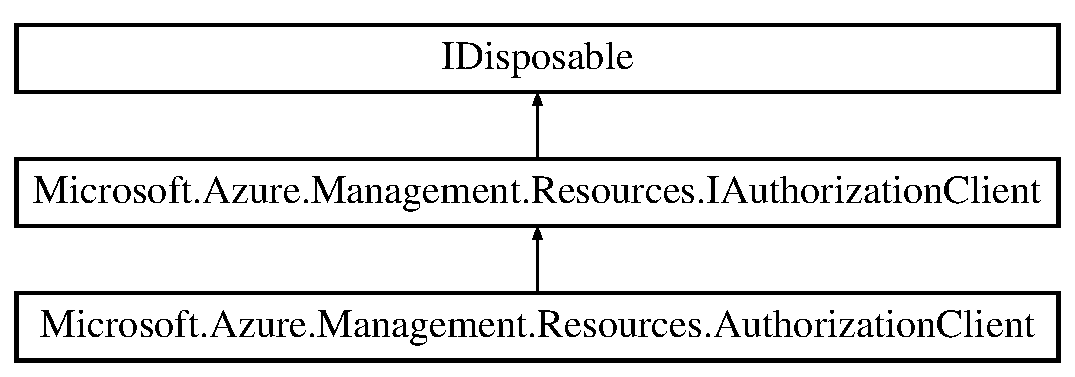
\includegraphics[height=3.000000cm]{interface_microsoft_1_1_azure_1_1_management_1_1_resources_1_1_i_authorization_client}
\end{center}
\end{figure}
\subsection*{Properties}
\begin{DoxyCompactItemize}
\item 
Uri \hyperlink{interface_microsoft_1_1_azure_1_1_management_1_1_resources_1_1_i_authorization_client_aa8a81e74caf17344db16fbf71cb3990e}{Base\+Uri}\hspace{0.3cm}{\ttfamily  \mbox{[}get, set\mbox{]}}
\begin{DoxyCompactList}\small\item\em The base U\+RI of the service. \end{DoxyCompactList}\item 
Json\+Serializer\+Settings \hyperlink{interface_microsoft_1_1_azure_1_1_management_1_1_resources_1_1_i_authorization_client_a6ab4feaa6a0065c2a6a60ada5bd60c87}{Serialization\+Settings}\hspace{0.3cm}{\ttfamily  \mbox{[}get\mbox{]}}
\begin{DoxyCompactList}\small\item\em Gets or sets json serialization settings. \end{DoxyCompactList}\item 
Json\+Serializer\+Settings \hyperlink{interface_microsoft_1_1_azure_1_1_management_1_1_resources_1_1_i_authorization_client_aba137ea69e7e92dea48720c5a37ad61c}{Deserialization\+Settings}\hspace{0.3cm}{\ttfamily  \mbox{[}get\mbox{]}}
\begin{DoxyCompactList}\small\item\em Gets or sets json deserialization settings. \end{DoxyCompactList}\item 
Service\+Client\+Credentials \hyperlink{interface_microsoft_1_1_azure_1_1_management_1_1_resources_1_1_i_authorization_client_a8b579613d22cac60f66ed68834b80f3d}{Credentials}\hspace{0.3cm}{\ttfamily  \mbox{[}get\mbox{]}}
\begin{DoxyCompactList}\small\item\em The management credentials for \hyperlink{namespace_microsoft_1_1_azure}{Azure}. \end{DoxyCompactList}\item 
string \hyperlink{interface_microsoft_1_1_azure_1_1_management_1_1_resources_1_1_i_authorization_client_a0d9b5f4063c29434136a96f5a7961a83}{Subscription\+Id}\hspace{0.3cm}{\ttfamily  \mbox{[}get, set\mbox{]}}
\begin{DoxyCompactList}\small\item\em Gets subscription credentials which uniquely identify \hyperlink{namespace_microsoft}{Microsoft} \hyperlink{namespace_microsoft_1_1_azure}{Azure} subscription. The subscription ID forms part of the U\+RI for every service call. \end{DoxyCompactList}\item 
string \hyperlink{interface_microsoft_1_1_azure_1_1_management_1_1_resources_1_1_i_authorization_client_af88a64d6177da1f76fe2db44e7d5d20d}{Api\+Version}\hspace{0.3cm}{\ttfamily  \mbox{[}get\mbox{]}}
\begin{DoxyCompactList}\small\item\em Client Api Version. \end{DoxyCompactList}\item 
string \hyperlink{interface_microsoft_1_1_azure_1_1_management_1_1_resources_1_1_i_authorization_client_a9886b312e9966ef74e7bf459cb2a4d7d}{Accept\+Language}\hspace{0.3cm}{\ttfamily  \mbox{[}get, set\mbox{]}}
\begin{DoxyCompactList}\small\item\em Gets or sets the preferred language for the response. \end{DoxyCompactList}\item 
int \hyperlink{interface_microsoft_1_1_azure_1_1_management_1_1_resources_1_1_i_authorization_client_a88a4000cd5c8e2077baabcb8ae8dfce9}{Long\+Running\+Operation\+Retry\+Timeout}\hspace{0.3cm}{\ttfamily  \mbox{[}get, set\mbox{]}}
\begin{DoxyCompactList}\small\item\em The retry timeout for Long Running Operations. \end{DoxyCompactList}\item 
\hyperlink{interface_microsoft_1_1_azure_1_1_management_1_1_resources_1_1_i_management_locks_operations}{I\+Management\+Locks\+Operations} {\bfseries Management\+Locks}\hspace{0.3cm}{\ttfamily  \mbox{[}get\mbox{]}}\hypertarget{interface_microsoft_1_1_azure_1_1_management_1_1_resources_1_1_i_authorization_client_ae3ee61ba759b13780fede3583e34bfc2}{}\label{interface_microsoft_1_1_azure_1_1_management_1_1_resources_1_1_i_authorization_client_ae3ee61ba759b13780fede3583e34bfc2}

\end{DoxyCompactItemize}


\subsection{Detailed Description}




\subsection{Property Documentation}
\index{Microsoft\+::\+Azure\+::\+Management\+::\+Resources\+::\+I\+Authorization\+Client@{Microsoft\+::\+Azure\+::\+Management\+::\+Resources\+::\+I\+Authorization\+Client}!Accept\+Language@{Accept\+Language}}
\index{Accept\+Language@{Accept\+Language}!Microsoft\+::\+Azure\+::\+Management\+::\+Resources\+::\+I\+Authorization\+Client@{Microsoft\+::\+Azure\+::\+Management\+::\+Resources\+::\+I\+Authorization\+Client}}
\subsubsection[{\texorpdfstring{Accept\+Language}{AcceptLanguage}}]{\setlength{\rightskip}{0pt plus 5cm}string Microsoft.\+Azure.\+Management.\+Resources.\+I\+Authorization\+Client.\+Accept\+Language\hspace{0.3cm}{\ttfamily [get]}, {\ttfamily [set]}}\hypertarget{interface_microsoft_1_1_azure_1_1_management_1_1_resources_1_1_i_authorization_client_a9886b312e9966ef74e7bf459cb2a4d7d}{}\label{interface_microsoft_1_1_azure_1_1_management_1_1_resources_1_1_i_authorization_client_a9886b312e9966ef74e7bf459cb2a4d7d}


Gets or sets the preferred language for the response. 

\index{Microsoft\+::\+Azure\+::\+Management\+::\+Resources\+::\+I\+Authorization\+Client@{Microsoft\+::\+Azure\+::\+Management\+::\+Resources\+::\+I\+Authorization\+Client}!Api\+Version@{Api\+Version}}
\index{Api\+Version@{Api\+Version}!Microsoft\+::\+Azure\+::\+Management\+::\+Resources\+::\+I\+Authorization\+Client@{Microsoft\+::\+Azure\+::\+Management\+::\+Resources\+::\+I\+Authorization\+Client}}
\subsubsection[{\texorpdfstring{Api\+Version}{ApiVersion}}]{\setlength{\rightskip}{0pt plus 5cm}string Microsoft.\+Azure.\+Management.\+Resources.\+I\+Authorization\+Client.\+Api\+Version\hspace{0.3cm}{\ttfamily [get]}}\hypertarget{interface_microsoft_1_1_azure_1_1_management_1_1_resources_1_1_i_authorization_client_af88a64d6177da1f76fe2db44e7d5d20d}{}\label{interface_microsoft_1_1_azure_1_1_management_1_1_resources_1_1_i_authorization_client_af88a64d6177da1f76fe2db44e7d5d20d}


Client Api Version. 

\index{Microsoft\+::\+Azure\+::\+Management\+::\+Resources\+::\+I\+Authorization\+Client@{Microsoft\+::\+Azure\+::\+Management\+::\+Resources\+::\+I\+Authorization\+Client}!Base\+Uri@{Base\+Uri}}
\index{Base\+Uri@{Base\+Uri}!Microsoft\+::\+Azure\+::\+Management\+::\+Resources\+::\+I\+Authorization\+Client@{Microsoft\+::\+Azure\+::\+Management\+::\+Resources\+::\+I\+Authorization\+Client}}
\subsubsection[{\texorpdfstring{Base\+Uri}{BaseUri}}]{\setlength{\rightskip}{0pt plus 5cm}Uri Microsoft.\+Azure.\+Management.\+Resources.\+I\+Authorization\+Client.\+Base\+Uri\hspace{0.3cm}{\ttfamily [get]}, {\ttfamily [set]}}\hypertarget{interface_microsoft_1_1_azure_1_1_management_1_1_resources_1_1_i_authorization_client_aa8a81e74caf17344db16fbf71cb3990e}{}\label{interface_microsoft_1_1_azure_1_1_management_1_1_resources_1_1_i_authorization_client_aa8a81e74caf17344db16fbf71cb3990e}


The base U\+RI of the service. 

\index{Microsoft\+::\+Azure\+::\+Management\+::\+Resources\+::\+I\+Authorization\+Client@{Microsoft\+::\+Azure\+::\+Management\+::\+Resources\+::\+I\+Authorization\+Client}!Credentials@{Credentials}}
\index{Credentials@{Credentials}!Microsoft\+::\+Azure\+::\+Management\+::\+Resources\+::\+I\+Authorization\+Client@{Microsoft\+::\+Azure\+::\+Management\+::\+Resources\+::\+I\+Authorization\+Client}}
\subsubsection[{\texorpdfstring{Credentials}{Credentials}}]{\setlength{\rightskip}{0pt plus 5cm}Service\+Client\+Credentials Microsoft.\+Azure.\+Management.\+Resources.\+I\+Authorization\+Client.\+Credentials\hspace{0.3cm}{\ttfamily [get]}}\hypertarget{interface_microsoft_1_1_azure_1_1_management_1_1_resources_1_1_i_authorization_client_a8b579613d22cac60f66ed68834b80f3d}{}\label{interface_microsoft_1_1_azure_1_1_management_1_1_resources_1_1_i_authorization_client_a8b579613d22cac60f66ed68834b80f3d}


The management credentials for \hyperlink{namespace_microsoft_1_1_azure}{Azure}. 

\index{Microsoft\+::\+Azure\+::\+Management\+::\+Resources\+::\+I\+Authorization\+Client@{Microsoft\+::\+Azure\+::\+Management\+::\+Resources\+::\+I\+Authorization\+Client}!Deserialization\+Settings@{Deserialization\+Settings}}
\index{Deserialization\+Settings@{Deserialization\+Settings}!Microsoft\+::\+Azure\+::\+Management\+::\+Resources\+::\+I\+Authorization\+Client@{Microsoft\+::\+Azure\+::\+Management\+::\+Resources\+::\+I\+Authorization\+Client}}
\subsubsection[{\texorpdfstring{Deserialization\+Settings}{DeserializationSettings}}]{\setlength{\rightskip}{0pt plus 5cm}Json\+Serializer\+Settings Microsoft.\+Azure.\+Management.\+Resources.\+I\+Authorization\+Client.\+Deserialization\+Settings\hspace{0.3cm}{\ttfamily [get]}}\hypertarget{interface_microsoft_1_1_azure_1_1_management_1_1_resources_1_1_i_authorization_client_aba137ea69e7e92dea48720c5a37ad61c}{}\label{interface_microsoft_1_1_azure_1_1_management_1_1_resources_1_1_i_authorization_client_aba137ea69e7e92dea48720c5a37ad61c}


Gets or sets json deserialization settings. 

\index{Microsoft\+::\+Azure\+::\+Management\+::\+Resources\+::\+I\+Authorization\+Client@{Microsoft\+::\+Azure\+::\+Management\+::\+Resources\+::\+I\+Authorization\+Client}!Long\+Running\+Operation\+Retry\+Timeout@{Long\+Running\+Operation\+Retry\+Timeout}}
\index{Long\+Running\+Operation\+Retry\+Timeout@{Long\+Running\+Operation\+Retry\+Timeout}!Microsoft\+::\+Azure\+::\+Management\+::\+Resources\+::\+I\+Authorization\+Client@{Microsoft\+::\+Azure\+::\+Management\+::\+Resources\+::\+I\+Authorization\+Client}}
\subsubsection[{\texorpdfstring{Long\+Running\+Operation\+Retry\+Timeout}{LongRunningOperationRetryTimeout}}]{\setlength{\rightskip}{0pt plus 5cm}int Microsoft.\+Azure.\+Management.\+Resources.\+I\+Authorization\+Client.\+Long\+Running\+Operation\+Retry\+Timeout\hspace{0.3cm}{\ttfamily [get]}, {\ttfamily [set]}}\hypertarget{interface_microsoft_1_1_azure_1_1_management_1_1_resources_1_1_i_authorization_client_a88a4000cd5c8e2077baabcb8ae8dfce9}{}\label{interface_microsoft_1_1_azure_1_1_management_1_1_resources_1_1_i_authorization_client_a88a4000cd5c8e2077baabcb8ae8dfce9}


The retry timeout for Long Running Operations. 

\index{Microsoft\+::\+Azure\+::\+Management\+::\+Resources\+::\+I\+Authorization\+Client@{Microsoft\+::\+Azure\+::\+Management\+::\+Resources\+::\+I\+Authorization\+Client}!Serialization\+Settings@{Serialization\+Settings}}
\index{Serialization\+Settings@{Serialization\+Settings}!Microsoft\+::\+Azure\+::\+Management\+::\+Resources\+::\+I\+Authorization\+Client@{Microsoft\+::\+Azure\+::\+Management\+::\+Resources\+::\+I\+Authorization\+Client}}
\subsubsection[{\texorpdfstring{Serialization\+Settings}{SerializationSettings}}]{\setlength{\rightskip}{0pt plus 5cm}Json\+Serializer\+Settings Microsoft.\+Azure.\+Management.\+Resources.\+I\+Authorization\+Client.\+Serialization\+Settings\hspace{0.3cm}{\ttfamily [get]}}\hypertarget{interface_microsoft_1_1_azure_1_1_management_1_1_resources_1_1_i_authorization_client_a6ab4feaa6a0065c2a6a60ada5bd60c87}{}\label{interface_microsoft_1_1_azure_1_1_management_1_1_resources_1_1_i_authorization_client_a6ab4feaa6a0065c2a6a60ada5bd60c87}


Gets or sets json serialization settings. 

\index{Microsoft\+::\+Azure\+::\+Management\+::\+Resources\+::\+I\+Authorization\+Client@{Microsoft\+::\+Azure\+::\+Management\+::\+Resources\+::\+I\+Authorization\+Client}!Subscription\+Id@{Subscription\+Id}}
\index{Subscription\+Id@{Subscription\+Id}!Microsoft\+::\+Azure\+::\+Management\+::\+Resources\+::\+I\+Authorization\+Client@{Microsoft\+::\+Azure\+::\+Management\+::\+Resources\+::\+I\+Authorization\+Client}}
\subsubsection[{\texorpdfstring{Subscription\+Id}{SubscriptionId}}]{\setlength{\rightskip}{0pt plus 5cm}string Microsoft.\+Azure.\+Management.\+Resources.\+I\+Authorization\+Client.\+Subscription\+Id\hspace{0.3cm}{\ttfamily [get]}, {\ttfamily [set]}}\hypertarget{interface_microsoft_1_1_azure_1_1_management_1_1_resources_1_1_i_authorization_client_a0d9b5f4063c29434136a96f5a7961a83}{}\label{interface_microsoft_1_1_azure_1_1_management_1_1_resources_1_1_i_authorization_client_a0d9b5f4063c29434136a96f5a7961a83}


Gets subscription credentials which uniquely identify \hyperlink{namespace_microsoft}{Microsoft} \hyperlink{namespace_microsoft_1_1_azure}{Azure} subscription. The subscription ID forms part of the U\+RI for every service call. 



The documentation for this interface was generated from the following file\+:\begin{DoxyCompactItemize}
\item 
files/I\+Authorization\+Client.\+cs\end{DoxyCompactItemize}

\hypertarget{interface_microsoft_1_1_azure_1_1_management_1_1_resources_1_1_i_deployment_operations_operations}{}\section{Microsoft.\+Azure.\+Management.\+Resources.\+I\+Deployment\+Operations\+Operations Interface Reference}
\label{interface_microsoft_1_1_azure_1_1_management_1_1_resources_1_1_i_deployment_operations_operations}\index{Microsoft.\+Azure.\+Management.\+Resources.\+I\+Deployment\+Operations\+Operations@{Microsoft.\+Azure.\+Management.\+Resources.\+I\+Deployment\+Operations\+Operations}}


Deployment\+Operations\+Operations operations.  




Inherited by Microsoft.\+Azure.\+Management.\+Resources.\+Deployment\+Operations\+Operations.

\subsection*{Public Member Functions}
\begin{DoxyCompactItemize}
\item 
Task$<$ Azure\+Operation\+Response$<$ Deployment\+Operation $>$ $>$ \hyperlink{interface_microsoft_1_1_azure_1_1_management_1_1_resources_1_1_i_deployment_operations_operations_ae80578def07219d0b48d609cbfe95706}{Get\+With\+Http\+Messages\+Async} (string resource\+Group\+Name, string deployment\+Name, string operation\+Id, Dictionary$<$ string, List$<$ string $>$$>$ custom\+Headers=null, Cancellation\+Token cancellation\+Token=default(Cancellation\+Token))
\begin{DoxyCompactList}\small\item\em Get a list of deployments operations. \end{DoxyCompactList}\item 
Task$<$ Azure\+Operation\+Response$<$ I\+Page$<$ Deployment\+Operation $>$ $>$ $>$ \hyperlink{interface_microsoft_1_1_azure_1_1_management_1_1_resources_1_1_i_deployment_operations_operations_acf1eb319eb9d4f32f7bad1c51cc1a26a}{List\+With\+Http\+Messages\+Async} (string resource\+Group\+Name, string deployment\+Name, int?top=default(int?), Dictionary$<$ string, List$<$ string $>$$>$ custom\+Headers=null, Cancellation\+Token cancellation\+Token=default(Cancellation\+Token))
\begin{DoxyCompactList}\small\item\em Gets a list of deployments operations. \end{DoxyCompactList}\item 
Task$<$ Azure\+Operation\+Response$<$ I\+Page$<$ Deployment\+Operation $>$ $>$ $>$ \hyperlink{interface_microsoft_1_1_azure_1_1_management_1_1_resources_1_1_i_deployment_operations_operations_afe2641bafcd0543b82d6faa599b3d588}{List\+Next\+With\+Http\+Messages\+Async} (string next\+Page\+Link, Dictionary$<$ string, List$<$ string $>$$>$ custom\+Headers=null, Cancellation\+Token cancellation\+Token=default(Cancellation\+Token))
\begin{DoxyCompactList}\small\item\em Gets a list of deployments operations. \end{DoxyCompactList}\end{DoxyCompactItemize}


\subsection{Detailed Description}
Deployment\+Operations\+Operations operations. 



\subsection{Member Function Documentation}
\index{Microsoft\+::\+Azure\+::\+Management\+::\+Resources\+::\+I\+Deployment\+Operations\+Operations@{Microsoft\+::\+Azure\+::\+Management\+::\+Resources\+::\+I\+Deployment\+Operations\+Operations}!Get\+With\+Http\+Messages\+Async@{Get\+With\+Http\+Messages\+Async}}
\index{Get\+With\+Http\+Messages\+Async@{Get\+With\+Http\+Messages\+Async}!Microsoft\+::\+Azure\+::\+Management\+::\+Resources\+::\+I\+Deployment\+Operations\+Operations@{Microsoft\+::\+Azure\+::\+Management\+::\+Resources\+::\+I\+Deployment\+Operations\+Operations}}
\subsubsection[{\texorpdfstring{Get\+With\+Http\+Messages\+Async(string resource\+Group\+Name, string deployment\+Name, string operation\+Id, Dictionary$<$ string, List$<$ string $>$$>$ custom\+Headers=null, Cancellation\+Token cancellation\+Token=default(\+Cancellation\+Token))}{GetWithHttpMessagesAsync(string resourceGroupName, string deploymentName, string operationId, Dictionary< string, List< string >> customHeaders=null, CancellationToken cancellationToken=default(CancellationToken))}}]{\setlength{\rightskip}{0pt plus 5cm}Task$<$Azure\+Operation\+Response$<$Deployment\+Operation$>$ $>$ Microsoft.\+Azure.\+Management.\+Resources.\+I\+Deployment\+Operations\+Operations.\+Get\+With\+Http\+Messages\+Async (
\begin{DoxyParamCaption}
\item[{string}]{resource\+Group\+Name, }
\item[{string}]{deployment\+Name, }
\item[{string}]{operation\+Id, }
\item[{Dictionary$<$ string, List$<$ string $>$$>$}]{custom\+Headers = {\ttfamily null}, }
\item[{Cancellation\+Token}]{cancellation\+Token = {\ttfamily default(CancellationToken)}}
\end{DoxyParamCaption}
)}\hypertarget{interface_microsoft_1_1_azure_1_1_management_1_1_resources_1_1_i_deployment_operations_operations_ae80578def07219d0b48d609cbfe95706}{}\label{interface_microsoft_1_1_azure_1_1_management_1_1_resources_1_1_i_deployment_operations_operations_ae80578def07219d0b48d609cbfe95706}


Get a list of deployments operations. 


\begin{DoxyParams}{Parameters}
{\em resource\+Group\+Name} & The name of the resource group. The name is case insensitive. \\
\hline
{\em deployment\+Name} & The name of the deployment. \\
\hline
{\em operation\+Id} & Operation Id. \\
\hline
{\em custom\+Headers} & The headers that will be added to request. \\
\hline
{\em cancellation\+Token} & The cancellation token. \\
\hline
\end{DoxyParams}
\index{Microsoft\+::\+Azure\+::\+Management\+::\+Resources\+::\+I\+Deployment\+Operations\+Operations@{Microsoft\+::\+Azure\+::\+Management\+::\+Resources\+::\+I\+Deployment\+Operations\+Operations}!List\+Next\+With\+Http\+Messages\+Async@{List\+Next\+With\+Http\+Messages\+Async}}
\index{List\+Next\+With\+Http\+Messages\+Async@{List\+Next\+With\+Http\+Messages\+Async}!Microsoft\+::\+Azure\+::\+Management\+::\+Resources\+::\+I\+Deployment\+Operations\+Operations@{Microsoft\+::\+Azure\+::\+Management\+::\+Resources\+::\+I\+Deployment\+Operations\+Operations}}
\subsubsection[{\texorpdfstring{List\+Next\+With\+Http\+Messages\+Async(string next\+Page\+Link, Dictionary$<$ string, List$<$ string $>$$>$ custom\+Headers=null, Cancellation\+Token cancellation\+Token=default(\+Cancellation\+Token))}{ListNextWithHttpMessagesAsync(string nextPageLink, Dictionary< string, List< string >> customHeaders=null, CancellationToken cancellationToken=default(CancellationToken))}}]{\setlength{\rightskip}{0pt plus 5cm}Task$<$Azure\+Operation\+Response$<$I\+Page$<$Deployment\+Operation$>$ $>$ $>$ Microsoft.\+Azure.\+Management.\+Resources.\+I\+Deployment\+Operations\+Operations.\+List\+Next\+With\+Http\+Messages\+Async (
\begin{DoxyParamCaption}
\item[{string}]{next\+Page\+Link, }
\item[{Dictionary$<$ string, List$<$ string $>$$>$}]{custom\+Headers = {\ttfamily null}, }
\item[{Cancellation\+Token}]{cancellation\+Token = {\ttfamily default(CancellationToken)}}
\end{DoxyParamCaption}
)}\hypertarget{interface_microsoft_1_1_azure_1_1_management_1_1_resources_1_1_i_deployment_operations_operations_afe2641bafcd0543b82d6faa599b3d588}{}\label{interface_microsoft_1_1_azure_1_1_management_1_1_resources_1_1_i_deployment_operations_operations_afe2641bafcd0543b82d6faa599b3d588}


Gets a list of deployments operations. 


\begin{DoxyParams}{Parameters}
{\em next\+Page\+Link} & The Next\+Link from the previous successful call to List operation. \\
\hline
{\em custom\+Headers} & The headers that will be added to request. \\
\hline
{\em cancellation\+Token} & The cancellation token. \\
\hline
\end{DoxyParams}
\index{Microsoft\+::\+Azure\+::\+Management\+::\+Resources\+::\+I\+Deployment\+Operations\+Operations@{Microsoft\+::\+Azure\+::\+Management\+::\+Resources\+::\+I\+Deployment\+Operations\+Operations}!List\+With\+Http\+Messages\+Async@{List\+With\+Http\+Messages\+Async}}
\index{List\+With\+Http\+Messages\+Async@{List\+With\+Http\+Messages\+Async}!Microsoft\+::\+Azure\+::\+Management\+::\+Resources\+::\+I\+Deployment\+Operations\+Operations@{Microsoft\+::\+Azure\+::\+Management\+::\+Resources\+::\+I\+Deployment\+Operations\+Operations}}
\subsubsection[{\texorpdfstring{List\+With\+Http\+Messages\+Async(string resource\+Group\+Name, string deployment\+Name, int?top=default(int?), Dictionary$<$ string, List$<$ string $>$$>$ custom\+Headers=null, Cancellation\+Token cancellation\+Token=default(\+Cancellation\+Token))}{ListWithHttpMessagesAsync(string resourceGroupName, string deploymentName, int?top=default(int?), Dictionary< string, List< string >> customHeaders=null, CancellationToken cancellationToken=default(CancellationToken))}}]{\setlength{\rightskip}{0pt plus 5cm}Task$<$Azure\+Operation\+Response$<$I\+Page$<$Deployment\+Operation$>$ $>$ $>$ Microsoft.\+Azure.\+Management.\+Resources.\+I\+Deployment\+Operations\+Operations.\+List\+With\+Http\+Messages\+Async (
\begin{DoxyParamCaption}
\item[{string}]{resource\+Group\+Name, }
\item[{string}]{deployment\+Name, }
\item[{int?}]{top = {\ttfamily default(int?)}, }
\item[{Dictionary$<$ string, List$<$ string $>$$>$}]{custom\+Headers = {\ttfamily null}, }
\item[{Cancellation\+Token}]{cancellation\+Token = {\ttfamily default(CancellationToken)}}
\end{DoxyParamCaption}
)}\hypertarget{interface_microsoft_1_1_azure_1_1_management_1_1_resources_1_1_i_deployment_operations_operations_acf1eb319eb9d4f32f7bad1c51cc1a26a}{}\label{interface_microsoft_1_1_azure_1_1_management_1_1_resources_1_1_i_deployment_operations_operations_acf1eb319eb9d4f32f7bad1c51cc1a26a}


Gets a list of deployments operations. 


\begin{DoxyParams}{Parameters}
{\em resource\+Group\+Name} & The name of the resource group. The name is case insensitive. \\
\hline
{\em deployment\+Name} & The name of the deployment. \\
\hline
{\em top} & Query parameters. \\
\hline
{\em custom\+Headers} & The headers that will be added to request. \\
\hline
{\em cancellation\+Token} & The cancellation token. \\
\hline
\end{DoxyParams}


The documentation for this interface was generated from the following file\+:\begin{DoxyCompactItemize}
\item 
files/I\+Deployment\+Operations\+Operations.\+cs\end{DoxyCompactItemize}

\hypertarget{interface_microsoft_1_1_azure_1_1_management_1_1_resources_1_1_i_deployments_operations}{}\section{Microsoft.\+Azure.\+Management.\+Resources.\+I\+Deployments\+Operations Interface Reference}
\label{interface_microsoft_1_1_azure_1_1_management_1_1_resources_1_1_i_deployments_operations}\index{Microsoft.\+Azure.\+Management.\+Resources.\+I\+Deployments\+Operations@{Microsoft.\+Azure.\+Management.\+Resources.\+I\+Deployments\+Operations}}


Deployments\+Operations operations.  




Inherited by Microsoft.\+Azure.\+Management.\+Resources.\+Deployments\+Operations.

\subsection*{Public Member Functions}
\begin{DoxyCompactItemize}
\item 
Task$<$ Azure\+Operation\+Response $>$ \hyperlink{interface_microsoft_1_1_azure_1_1_management_1_1_resources_1_1_i_deployments_operations_a2f60c8afe521264fde75d8d932297df9}{Delete\+With\+Http\+Messages\+Async} (string resource\+Group\+Name, string deployment\+Name, Dictionary$<$ string, List$<$ string $>$$>$ custom\+Headers=null, Cancellation\+Token cancellation\+Token=default(Cancellation\+Token))
\begin{DoxyCompactList}\small\item\em Begin deleting deployment.\+To determine whether the operation has finished processing the request, call Get\+Long\+Running\+Operation\+Status. \end{DoxyCompactList}\item 
Task$<$ Azure\+Operation\+Response $>$ \hyperlink{interface_microsoft_1_1_azure_1_1_management_1_1_resources_1_1_i_deployments_operations_ac40e576289a92a4ca19094778ff73ca4}{Begin\+Delete\+With\+Http\+Messages\+Async} (string resource\+Group\+Name, string deployment\+Name, Dictionary$<$ string, List$<$ string $>$$>$ custom\+Headers=null, Cancellation\+Token cancellation\+Token=default(Cancellation\+Token))
\begin{DoxyCompactList}\small\item\em Begin deleting deployment.\+To determine whether the operation has finished processing the request, call Get\+Long\+Running\+Operation\+Status. \end{DoxyCompactList}\item 
Task$<$ Azure\+Operation\+Response$<$ bool?$>$ $>$ \hyperlink{interface_microsoft_1_1_azure_1_1_management_1_1_resources_1_1_i_deployments_operations_a809179e8e439d8c237c81fb67c9fb502}{Check\+Existence\+With\+Http\+Messages\+Async} (string resource\+Group\+Name, string deployment\+Name, Dictionary$<$ string, List$<$ string $>$$>$ custom\+Headers=null, Cancellation\+Token cancellation\+Token=default(Cancellation\+Token))
\begin{DoxyCompactList}\small\item\em Checks whether deployment exists. \end{DoxyCompactList}\item 
Task$<$ Azure\+Operation\+Response$<$ Deployment\+Extended $>$ $>$ \hyperlink{interface_microsoft_1_1_azure_1_1_management_1_1_resources_1_1_i_deployments_operations_a37f3c71c9c2e4089aa73bcf3ef4a44d7}{Create\+Or\+Update\+With\+Http\+Messages\+Async} (string resource\+Group\+Name, string deployment\+Name, Deployment parameters, Dictionary$<$ string, List$<$ string $>$$>$ custom\+Headers=null, Cancellation\+Token cancellation\+Token=default(Cancellation\+Token))
\begin{DoxyCompactList}\small\item\em Create a named template deployment using a template. \end{DoxyCompactList}\item 
Task$<$ Azure\+Operation\+Response$<$ Deployment\+Extended $>$ $>$ \hyperlink{interface_microsoft_1_1_azure_1_1_management_1_1_resources_1_1_i_deployments_operations_a7e7bd5ff46eaf9e224b197ad45925f11}{Begin\+Create\+Or\+Update\+With\+Http\+Messages\+Async} (string resource\+Group\+Name, string deployment\+Name, Deployment parameters, Dictionary$<$ string, List$<$ string $>$$>$ custom\+Headers=null, Cancellation\+Token cancellation\+Token=default(Cancellation\+Token))
\begin{DoxyCompactList}\small\item\em Create a named template deployment using a template. \end{DoxyCompactList}\item 
Task$<$ Azure\+Operation\+Response$<$ Deployment\+Extended $>$ $>$ \hyperlink{interface_microsoft_1_1_azure_1_1_management_1_1_resources_1_1_i_deployments_operations_a3e1f85b3b65f1409d1562160693ff1ed}{Get\+With\+Http\+Messages\+Async} (string resource\+Group\+Name, string deployment\+Name, Dictionary$<$ string, List$<$ string $>$$>$ custom\+Headers=null, Cancellation\+Token cancellation\+Token=default(Cancellation\+Token))
\begin{DoxyCompactList}\small\item\em Get a deployment. \end{DoxyCompactList}\item 
Task$<$ Azure\+Operation\+Response $>$ \hyperlink{interface_microsoft_1_1_azure_1_1_management_1_1_resources_1_1_i_deployments_operations_aba50ee2e15688eb10a33236b52812969}{Cancel\+With\+Http\+Messages\+Async} (string resource\+Group\+Name, string deployment\+Name, Dictionary$<$ string, List$<$ string $>$$>$ custom\+Headers=null, Cancellation\+Token cancellation\+Token=default(Cancellation\+Token))
\begin{DoxyCompactList}\small\item\em Cancel a currently running template deployment. \end{DoxyCompactList}\item 
Task$<$ Azure\+Operation\+Response$<$ Deployment\+Validate\+Result $>$ $>$ \hyperlink{interface_microsoft_1_1_azure_1_1_management_1_1_resources_1_1_i_deployments_operations_a768f02de88ae476438aedb2716df10d6}{Validate\+With\+Http\+Messages\+Async} (string resource\+Group\+Name, string deployment\+Name, Deployment parameters, Dictionary$<$ string, List$<$ string $>$$>$ custom\+Headers=null, Cancellation\+Token cancellation\+Token=default(Cancellation\+Token))
\begin{DoxyCompactList}\small\item\em Validate a deployment template. \end{DoxyCompactList}\item 
Task$<$ Azure\+Operation\+Response$<$ I\+Page$<$ Deployment\+Extended $>$ $>$ $>$ \hyperlink{interface_microsoft_1_1_azure_1_1_management_1_1_resources_1_1_i_deployments_operations_a5c19611a775bc858103ff85f3b487bb9}{List\+With\+Http\+Messages\+Async} (string resource\+Group\+Name, O\+Data\+Query$<$ Deployment\+Extended\+Filter $>$ odata\+Query=default(O\+Data\+Query$<$ Deployment\+Extended\+Filter $>$), Dictionary$<$ string, List$<$ string $>$$>$ custom\+Headers=null, Cancellation\+Token cancellation\+Token=default(Cancellation\+Token))
\begin{DoxyCompactList}\small\item\em Get a list of deployments. \end{DoxyCompactList}\item 
Task$<$ Azure\+Operation\+Response$<$ I\+Page$<$ Deployment\+Extended $>$ $>$ $>$ \hyperlink{interface_microsoft_1_1_azure_1_1_management_1_1_resources_1_1_i_deployments_operations_a5489b13cf77a2aedd15a435cc06d022e}{List\+Next\+With\+Http\+Messages\+Async} (string next\+Page\+Link, Dictionary$<$ string, List$<$ string $>$$>$ custom\+Headers=null, Cancellation\+Token cancellation\+Token=default(Cancellation\+Token))
\begin{DoxyCompactList}\small\item\em Get a list of deployments. \end{DoxyCompactList}\end{DoxyCompactItemize}


\subsection{Detailed Description}
Deployments\+Operations operations. 



\subsection{Member Function Documentation}
\index{Microsoft\+::\+Azure\+::\+Management\+::\+Resources\+::\+I\+Deployments\+Operations@{Microsoft\+::\+Azure\+::\+Management\+::\+Resources\+::\+I\+Deployments\+Operations}!Begin\+Create\+Or\+Update\+With\+Http\+Messages\+Async@{Begin\+Create\+Or\+Update\+With\+Http\+Messages\+Async}}
\index{Begin\+Create\+Or\+Update\+With\+Http\+Messages\+Async@{Begin\+Create\+Or\+Update\+With\+Http\+Messages\+Async}!Microsoft\+::\+Azure\+::\+Management\+::\+Resources\+::\+I\+Deployments\+Operations@{Microsoft\+::\+Azure\+::\+Management\+::\+Resources\+::\+I\+Deployments\+Operations}}
\subsubsection[{\texorpdfstring{Begin\+Create\+Or\+Update\+With\+Http\+Messages\+Async(string resource\+Group\+Name, string deployment\+Name, Deployment parameters, Dictionary$<$ string, List$<$ string $>$$>$ custom\+Headers=null, Cancellation\+Token cancellation\+Token=default(\+Cancellation\+Token))}{BeginCreateOrUpdateWithHttpMessagesAsync(string resourceGroupName, string deploymentName, Deployment parameters, Dictionary< string, List< string >> customHeaders=null, CancellationToken cancellationToken=default(CancellationToken))}}]{\setlength{\rightskip}{0pt plus 5cm}Task$<$Azure\+Operation\+Response$<$Deployment\+Extended$>$ $>$ Microsoft.\+Azure.\+Management.\+Resources.\+I\+Deployments\+Operations.\+Begin\+Create\+Or\+Update\+With\+Http\+Messages\+Async (
\begin{DoxyParamCaption}
\item[{string}]{resource\+Group\+Name, }
\item[{string}]{deployment\+Name, }
\item[{Deployment}]{parameters, }
\item[{Dictionary$<$ string, List$<$ string $>$$>$}]{custom\+Headers = {\ttfamily null}, }
\item[{Cancellation\+Token}]{cancellation\+Token = {\ttfamily default(CancellationToken)}}
\end{DoxyParamCaption}
)}\hypertarget{interface_microsoft_1_1_azure_1_1_management_1_1_resources_1_1_i_deployments_operations_a7e7bd5ff46eaf9e224b197ad45925f11}{}\label{interface_microsoft_1_1_azure_1_1_management_1_1_resources_1_1_i_deployments_operations_a7e7bd5ff46eaf9e224b197ad45925f11}


Create a named template deployment using a template. 


\begin{DoxyParams}{Parameters}
{\em resource\+Group\+Name} & The name of the resource group. The name is case insensitive. \\
\hline
{\em deployment\+Name} & The name of the deployment. \\
\hline
{\em parameters} & Additional parameters supplied to the operation. \\
\hline
{\em custom\+Headers} & The headers that will be added to request. \\
\hline
{\em cancellation\+Token} & The cancellation token. \\
\hline
\end{DoxyParams}
\index{Microsoft\+::\+Azure\+::\+Management\+::\+Resources\+::\+I\+Deployments\+Operations@{Microsoft\+::\+Azure\+::\+Management\+::\+Resources\+::\+I\+Deployments\+Operations}!Begin\+Delete\+With\+Http\+Messages\+Async@{Begin\+Delete\+With\+Http\+Messages\+Async}}
\index{Begin\+Delete\+With\+Http\+Messages\+Async@{Begin\+Delete\+With\+Http\+Messages\+Async}!Microsoft\+::\+Azure\+::\+Management\+::\+Resources\+::\+I\+Deployments\+Operations@{Microsoft\+::\+Azure\+::\+Management\+::\+Resources\+::\+I\+Deployments\+Operations}}
\subsubsection[{\texorpdfstring{Begin\+Delete\+With\+Http\+Messages\+Async(string resource\+Group\+Name, string deployment\+Name, Dictionary$<$ string, List$<$ string $>$$>$ custom\+Headers=null, Cancellation\+Token cancellation\+Token=default(\+Cancellation\+Token))}{BeginDeleteWithHttpMessagesAsync(string resourceGroupName, string deploymentName, Dictionary< string, List< string >> customHeaders=null, CancellationToken cancellationToken=default(CancellationToken))}}]{\setlength{\rightskip}{0pt plus 5cm}Task$<$Azure\+Operation\+Response$>$ Microsoft.\+Azure.\+Management.\+Resources.\+I\+Deployments\+Operations.\+Begin\+Delete\+With\+Http\+Messages\+Async (
\begin{DoxyParamCaption}
\item[{string}]{resource\+Group\+Name, }
\item[{string}]{deployment\+Name, }
\item[{Dictionary$<$ string, List$<$ string $>$$>$}]{custom\+Headers = {\ttfamily null}, }
\item[{Cancellation\+Token}]{cancellation\+Token = {\ttfamily default(CancellationToken)}}
\end{DoxyParamCaption}
)}\hypertarget{interface_microsoft_1_1_azure_1_1_management_1_1_resources_1_1_i_deployments_operations_ac40e576289a92a4ca19094778ff73ca4}{}\label{interface_microsoft_1_1_azure_1_1_management_1_1_resources_1_1_i_deployments_operations_ac40e576289a92a4ca19094778ff73ca4}


Begin deleting deployment.\+To determine whether the operation has finished processing the request, call Get\+Long\+Running\+Operation\+Status. 


\begin{DoxyParams}{Parameters}
{\em resource\+Group\+Name} & The name of the resource group. The name is case insensitive. \\
\hline
{\em deployment\+Name} & The name of the deployment to be deleted. \\
\hline
{\em custom\+Headers} & The headers that will be added to request. \\
\hline
{\em cancellation\+Token} & The cancellation token. \\
\hline
\end{DoxyParams}
\index{Microsoft\+::\+Azure\+::\+Management\+::\+Resources\+::\+I\+Deployments\+Operations@{Microsoft\+::\+Azure\+::\+Management\+::\+Resources\+::\+I\+Deployments\+Operations}!Cancel\+With\+Http\+Messages\+Async@{Cancel\+With\+Http\+Messages\+Async}}
\index{Cancel\+With\+Http\+Messages\+Async@{Cancel\+With\+Http\+Messages\+Async}!Microsoft\+::\+Azure\+::\+Management\+::\+Resources\+::\+I\+Deployments\+Operations@{Microsoft\+::\+Azure\+::\+Management\+::\+Resources\+::\+I\+Deployments\+Operations}}
\subsubsection[{\texorpdfstring{Cancel\+With\+Http\+Messages\+Async(string resource\+Group\+Name, string deployment\+Name, Dictionary$<$ string, List$<$ string $>$$>$ custom\+Headers=null, Cancellation\+Token cancellation\+Token=default(\+Cancellation\+Token))}{CancelWithHttpMessagesAsync(string resourceGroupName, string deploymentName, Dictionary< string, List< string >> customHeaders=null, CancellationToken cancellationToken=default(CancellationToken))}}]{\setlength{\rightskip}{0pt plus 5cm}Task$<$Azure\+Operation\+Response$>$ Microsoft.\+Azure.\+Management.\+Resources.\+I\+Deployments\+Operations.\+Cancel\+With\+Http\+Messages\+Async (
\begin{DoxyParamCaption}
\item[{string}]{resource\+Group\+Name, }
\item[{string}]{deployment\+Name, }
\item[{Dictionary$<$ string, List$<$ string $>$$>$}]{custom\+Headers = {\ttfamily null}, }
\item[{Cancellation\+Token}]{cancellation\+Token = {\ttfamily default(CancellationToken)}}
\end{DoxyParamCaption}
)}\hypertarget{interface_microsoft_1_1_azure_1_1_management_1_1_resources_1_1_i_deployments_operations_aba50ee2e15688eb10a33236b52812969}{}\label{interface_microsoft_1_1_azure_1_1_management_1_1_resources_1_1_i_deployments_operations_aba50ee2e15688eb10a33236b52812969}


Cancel a currently running template deployment. 


\begin{DoxyParams}{Parameters}
{\em resource\+Group\+Name} & The name of the resource group. The name is case insensitive. \\
\hline
{\em deployment\+Name} & The name of the deployment. \\
\hline
{\em custom\+Headers} & The headers that will be added to request. \\
\hline
{\em cancellation\+Token} & The cancellation token. \\
\hline
\end{DoxyParams}
\index{Microsoft\+::\+Azure\+::\+Management\+::\+Resources\+::\+I\+Deployments\+Operations@{Microsoft\+::\+Azure\+::\+Management\+::\+Resources\+::\+I\+Deployments\+Operations}!Check\+Existence\+With\+Http\+Messages\+Async@{Check\+Existence\+With\+Http\+Messages\+Async}}
\index{Check\+Existence\+With\+Http\+Messages\+Async@{Check\+Existence\+With\+Http\+Messages\+Async}!Microsoft\+::\+Azure\+::\+Management\+::\+Resources\+::\+I\+Deployments\+Operations@{Microsoft\+::\+Azure\+::\+Management\+::\+Resources\+::\+I\+Deployments\+Operations}}
\subsubsection[{\texorpdfstring{Check\+Existence\+With\+Http\+Messages\+Async(string resource\+Group\+Name, string deployment\+Name, Dictionary$<$ string, List$<$ string $>$$>$ custom\+Headers=null, Cancellation\+Token cancellation\+Token=default(\+Cancellation\+Token))}{CheckExistenceWithHttpMessagesAsync(string resourceGroupName, string deploymentName, Dictionary< string, List< string >> customHeaders=null, CancellationToken cancellationToken=default(CancellationToken))}}]{\setlength{\rightskip}{0pt plus 5cm}Task$<$Azure\+Operation\+Response$<$bool?$>$ $>$ Microsoft.\+Azure.\+Management.\+Resources.\+I\+Deployments\+Operations.\+Check\+Existence\+With\+Http\+Messages\+Async (
\begin{DoxyParamCaption}
\item[{string}]{resource\+Group\+Name, }
\item[{string}]{deployment\+Name, }
\item[{Dictionary$<$ string, List$<$ string $>$$>$}]{custom\+Headers = {\ttfamily null}, }
\item[{Cancellation\+Token}]{cancellation\+Token = {\ttfamily default(CancellationToken)}}
\end{DoxyParamCaption}
)}\hypertarget{interface_microsoft_1_1_azure_1_1_management_1_1_resources_1_1_i_deployments_operations_a809179e8e439d8c237c81fb67c9fb502}{}\label{interface_microsoft_1_1_azure_1_1_management_1_1_resources_1_1_i_deployments_operations_a809179e8e439d8c237c81fb67c9fb502}


Checks whether deployment exists. 


\begin{DoxyParams}{Parameters}
{\em resource\+Group\+Name} & The name of the resource group to check. The name is case insensitive. \\
\hline
{\em deployment\+Name} & The name of the deployment. \\
\hline
{\em custom\+Headers} & The headers that will be added to request. \\
\hline
{\em cancellation\+Token} & The cancellation token. \\
\hline
\end{DoxyParams}
\index{Microsoft\+::\+Azure\+::\+Management\+::\+Resources\+::\+I\+Deployments\+Operations@{Microsoft\+::\+Azure\+::\+Management\+::\+Resources\+::\+I\+Deployments\+Operations}!Create\+Or\+Update\+With\+Http\+Messages\+Async@{Create\+Or\+Update\+With\+Http\+Messages\+Async}}
\index{Create\+Or\+Update\+With\+Http\+Messages\+Async@{Create\+Or\+Update\+With\+Http\+Messages\+Async}!Microsoft\+::\+Azure\+::\+Management\+::\+Resources\+::\+I\+Deployments\+Operations@{Microsoft\+::\+Azure\+::\+Management\+::\+Resources\+::\+I\+Deployments\+Operations}}
\subsubsection[{\texorpdfstring{Create\+Or\+Update\+With\+Http\+Messages\+Async(string resource\+Group\+Name, string deployment\+Name, Deployment parameters, Dictionary$<$ string, List$<$ string $>$$>$ custom\+Headers=null, Cancellation\+Token cancellation\+Token=default(\+Cancellation\+Token))}{CreateOrUpdateWithHttpMessagesAsync(string resourceGroupName, string deploymentName, Deployment parameters, Dictionary< string, List< string >> customHeaders=null, CancellationToken cancellationToken=default(CancellationToken))}}]{\setlength{\rightskip}{0pt plus 5cm}Task$<$Azure\+Operation\+Response$<$Deployment\+Extended$>$ $>$ Microsoft.\+Azure.\+Management.\+Resources.\+I\+Deployments\+Operations.\+Create\+Or\+Update\+With\+Http\+Messages\+Async (
\begin{DoxyParamCaption}
\item[{string}]{resource\+Group\+Name, }
\item[{string}]{deployment\+Name, }
\item[{Deployment}]{parameters, }
\item[{Dictionary$<$ string, List$<$ string $>$$>$}]{custom\+Headers = {\ttfamily null}, }
\item[{Cancellation\+Token}]{cancellation\+Token = {\ttfamily default(CancellationToken)}}
\end{DoxyParamCaption}
)}\hypertarget{interface_microsoft_1_1_azure_1_1_management_1_1_resources_1_1_i_deployments_operations_a37f3c71c9c2e4089aa73bcf3ef4a44d7}{}\label{interface_microsoft_1_1_azure_1_1_management_1_1_resources_1_1_i_deployments_operations_a37f3c71c9c2e4089aa73bcf3ef4a44d7}


Create a named template deployment using a template. 


\begin{DoxyParams}{Parameters}
{\em resource\+Group\+Name} & The name of the resource group. The name is case insensitive. \\
\hline
{\em deployment\+Name} & The name of the deployment. \\
\hline
{\em parameters} & Additional parameters supplied to the operation. \\
\hline
{\em custom\+Headers} & The headers that will be added to request. \\
\hline
{\em cancellation\+Token} & The cancellation token. \\
\hline
\end{DoxyParams}
\index{Microsoft\+::\+Azure\+::\+Management\+::\+Resources\+::\+I\+Deployments\+Operations@{Microsoft\+::\+Azure\+::\+Management\+::\+Resources\+::\+I\+Deployments\+Operations}!Delete\+With\+Http\+Messages\+Async@{Delete\+With\+Http\+Messages\+Async}}
\index{Delete\+With\+Http\+Messages\+Async@{Delete\+With\+Http\+Messages\+Async}!Microsoft\+::\+Azure\+::\+Management\+::\+Resources\+::\+I\+Deployments\+Operations@{Microsoft\+::\+Azure\+::\+Management\+::\+Resources\+::\+I\+Deployments\+Operations}}
\subsubsection[{\texorpdfstring{Delete\+With\+Http\+Messages\+Async(string resource\+Group\+Name, string deployment\+Name, Dictionary$<$ string, List$<$ string $>$$>$ custom\+Headers=null, Cancellation\+Token cancellation\+Token=default(\+Cancellation\+Token))}{DeleteWithHttpMessagesAsync(string resourceGroupName, string deploymentName, Dictionary< string, List< string >> customHeaders=null, CancellationToken cancellationToken=default(CancellationToken))}}]{\setlength{\rightskip}{0pt plus 5cm}Task$<$Azure\+Operation\+Response$>$ Microsoft.\+Azure.\+Management.\+Resources.\+I\+Deployments\+Operations.\+Delete\+With\+Http\+Messages\+Async (
\begin{DoxyParamCaption}
\item[{string}]{resource\+Group\+Name, }
\item[{string}]{deployment\+Name, }
\item[{Dictionary$<$ string, List$<$ string $>$$>$}]{custom\+Headers = {\ttfamily null}, }
\item[{Cancellation\+Token}]{cancellation\+Token = {\ttfamily default(CancellationToken)}}
\end{DoxyParamCaption}
)}\hypertarget{interface_microsoft_1_1_azure_1_1_management_1_1_resources_1_1_i_deployments_operations_a2f60c8afe521264fde75d8d932297df9}{}\label{interface_microsoft_1_1_azure_1_1_management_1_1_resources_1_1_i_deployments_operations_a2f60c8afe521264fde75d8d932297df9}


Begin deleting deployment.\+To determine whether the operation has finished processing the request, call Get\+Long\+Running\+Operation\+Status. 


\begin{DoxyParams}{Parameters}
{\em resource\+Group\+Name} & The name of the resource group. The name is case insensitive. \\
\hline
{\em deployment\+Name} & The name of the deployment to be deleted. \\
\hline
{\em custom\+Headers} & The headers that will be added to request. \\
\hline
{\em cancellation\+Token} & The cancellation token. \\
\hline
\end{DoxyParams}
\index{Microsoft\+::\+Azure\+::\+Management\+::\+Resources\+::\+I\+Deployments\+Operations@{Microsoft\+::\+Azure\+::\+Management\+::\+Resources\+::\+I\+Deployments\+Operations}!Get\+With\+Http\+Messages\+Async@{Get\+With\+Http\+Messages\+Async}}
\index{Get\+With\+Http\+Messages\+Async@{Get\+With\+Http\+Messages\+Async}!Microsoft\+::\+Azure\+::\+Management\+::\+Resources\+::\+I\+Deployments\+Operations@{Microsoft\+::\+Azure\+::\+Management\+::\+Resources\+::\+I\+Deployments\+Operations}}
\subsubsection[{\texorpdfstring{Get\+With\+Http\+Messages\+Async(string resource\+Group\+Name, string deployment\+Name, Dictionary$<$ string, List$<$ string $>$$>$ custom\+Headers=null, Cancellation\+Token cancellation\+Token=default(\+Cancellation\+Token))}{GetWithHttpMessagesAsync(string resourceGroupName, string deploymentName, Dictionary< string, List< string >> customHeaders=null, CancellationToken cancellationToken=default(CancellationToken))}}]{\setlength{\rightskip}{0pt plus 5cm}Task$<$Azure\+Operation\+Response$<$Deployment\+Extended$>$ $>$ Microsoft.\+Azure.\+Management.\+Resources.\+I\+Deployments\+Operations.\+Get\+With\+Http\+Messages\+Async (
\begin{DoxyParamCaption}
\item[{string}]{resource\+Group\+Name, }
\item[{string}]{deployment\+Name, }
\item[{Dictionary$<$ string, List$<$ string $>$$>$}]{custom\+Headers = {\ttfamily null}, }
\item[{Cancellation\+Token}]{cancellation\+Token = {\ttfamily default(CancellationToken)}}
\end{DoxyParamCaption}
)}\hypertarget{interface_microsoft_1_1_azure_1_1_management_1_1_resources_1_1_i_deployments_operations_a3e1f85b3b65f1409d1562160693ff1ed}{}\label{interface_microsoft_1_1_azure_1_1_management_1_1_resources_1_1_i_deployments_operations_a3e1f85b3b65f1409d1562160693ff1ed}


Get a deployment. 


\begin{DoxyParams}{Parameters}
{\em resource\+Group\+Name} & The name of the resource group to get. The name is case insensitive. \\
\hline
{\em deployment\+Name} & The name of the deployment. \\
\hline
{\em custom\+Headers} & The headers that will be added to request. \\
\hline
{\em cancellation\+Token} & The cancellation token. \\
\hline
\end{DoxyParams}
\index{Microsoft\+::\+Azure\+::\+Management\+::\+Resources\+::\+I\+Deployments\+Operations@{Microsoft\+::\+Azure\+::\+Management\+::\+Resources\+::\+I\+Deployments\+Operations}!List\+Next\+With\+Http\+Messages\+Async@{List\+Next\+With\+Http\+Messages\+Async}}
\index{List\+Next\+With\+Http\+Messages\+Async@{List\+Next\+With\+Http\+Messages\+Async}!Microsoft\+::\+Azure\+::\+Management\+::\+Resources\+::\+I\+Deployments\+Operations@{Microsoft\+::\+Azure\+::\+Management\+::\+Resources\+::\+I\+Deployments\+Operations}}
\subsubsection[{\texorpdfstring{List\+Next\+With\+Http\+Messages\+Async(string next\+Page\+Link, Dictionary$<$ string, List$<$ string $>$$>$ custom\+Headers=null, Cancellation\+Token cancellation\+Token=default(\+Cancellation\+Token))}{ListNextWithHttpMessagesAsync(string nextPageLink, Dictionary< string, List< string >> customHeaders=null, CancellationToken cancellationToken=default(CancellationToken))}}]{\setlength{\rightskip}{0pt plus 5cm}Task$<$Azure\+Operation\+Response$<$I\+Page$<$Deployment\+Extended$>$ $>$ $>$ Microsoft.\+Azure.\+Management.\+Resources.\+I\+Deployments\+Operations.\+List\+Next\+With\+Http\+Messages\+Async (
\begin{DoxyParamCaption}
\item[{string}]{next\+Page\+Link, }
\item[{Dictionary$<$ string, List$<$ string $>$$>$}]{custom\+Headers = {\ttfamily null}, }
\item[{Cancellation\+Token}]{cancellation\+Token = {\ttfamily default(CancellationToken)}}
\end{DoxyParamCaption}
)}\hypertarget{interface_microsoft_1_1_azure_1_1_management_1_1_resources_1_1_i_deployments_operations_a5489b13cf77a2aedd15a435cc06d022e}{}\label{interface_microsoft_1_1_azure_1_1_management_1_1_resources_1_1_i_deployments_operations_a5489b13cf77a2aedd15a435cc06d022e}


Get a list of deployments. 


\begin{DoxyParams}{Parameters}
{\em next\+Page\+Link} & The Next\+Link from the previous successful call to List operation. \\
\hline
{\em custom\+Headers} & The headers that will be added to request. \\
\hline
{\em cancellation\+Token} & The cancellation token. \\
\hline
\end{DoxyParams}
\index{Microsoft\+::\+Azure\+::\+Management\+::\+Resources\+::\+I\+Deployments\+Operations@{Microsoft\+::\+Azure\+::\+Management\+::\+Resources\+::\+I\+Deployments\+Operations}!List\+With\+Http\+Messages\+Async@{List\+With\+Http\+Messages\+Async}}
\index{List\+With\+Http\+Messages\+Async@{List\+With\+Http\+Messages\+Async}!Microsoft\+::\+Azure\+::\+Management\+::\+Resources\+::\+I\+Deployments\+Operations@{Microsoft\+::\+Azure\+::\+Management\+::\+Resources\+::\+I\+Deployments\+Operations}}
\subsubsection[{\texorpdfstring{List\+With\+Http\+Messages\+Async(string resource\+Group\+Name, O\+Data\+Query$<$ Deployment\+Extended\+Filter $>$ odata\+Query=default(\+O\+Data\+Query$<$ Deployment\+Extended\+Filter $>$), Dictionary$<$ string, List$<$ string $>$$>$ custom\+Headers=null, Cancellation\+Token cancellation\+Token=default(\+Cancellation\+Token))}{ListWithHttpMessagesAsync(string resourceGroupName, ODataQuery< DeploymentExtendedFilter > odataQuery=default(ODataQuery< DeploymentExtendedFilter >), Dictionary< string, List< string >> customHeaders=null, CancellationToken cancellationToken=default(CancellationToken))}}]{\setlength{\rightskip}{0pt plus 5cm}Task$<$Azure\+Operation\+Response$<$I\+Page$<$Deployment\+Extended$>$ $>$ $>$ Microsoft.\+Azure.\+Management.\+Resources.\+I\+Deployments\+Operations.\+List\+With\+Http\+Messages\+Async (
\begin{DoxyParamCaption}
\item[{string}]{resource\+Group\+Name, }
\item[{O\+Data\+Query$<$ Deployment\+Extended\+Filter $>$}]{odata\+Query = {\ttfamily default(ODataQuery$<$~DeploymentExtendedFilter~$>$)}, }
\item[{Dictionary$<$ string, List$<$ string $>$$>$}]{custom\+Headers = {\ttfamily null}, }
\item[{Cancellation\+Token}]{cancellation\+Token = {\ttfamily default(CancellationToken)}}
\end{DoxyParamCaption}
)}\hypertarget{interface_microsoft_1_1_azure_1_1_management_1_1_resources_1_1_i_deployments_operations_a5c19611a775bc858103ff85f3b487bb9}{}\label{interface_microsoft_1_1_azure_1_1_management_1_1_resources_1_1_i_deployments_operations_a5c19611a775bc858103ff85f3b487bb9}


Get a list of deployments. 


\begin{DoxyParams}{Parameters}
{\em resource\+Group\+Name} & The name of the resource group to filter by. The name is case insensitive. \\
\hline
{\em odata\+Query} & O\+Data parameters to apply to the operation. \\
\hline
{\em custom\+Headers} & The headers that will be added to request. \\
\hline
{\em cancellation\+Token} & The cancellation token. \\
\hline
\end{DoxyParams}
\index{Microsoft\+::\+Azure\+::\+Management\+::\+Resources\+::\+I\+Deployments\+Operations@{Microsoft\+::\+Azure\+::\+Management\+::\+Resources\+::\+I\+Deployments\+Operations}!Validate\+With\+Http\+Messages\+Async@{Validate\+With\+Http\+Messages\+Async}}
\index{Validate\+With\+Http\+Messages\+Async@{Validate\+With\+Http\+Messages\+Async}!Microsoft\+::\+Azure\+::\+Management\+::\+Resources\+::\+I\+Deployments\+Operations@{Microsoft\+::\+Azure\+::\+Management\+::\+Resources\+::\+I\+Deployments\+Operations}}
\subsubsection[{\texorpdfstring{Validate\+With\+Http\+Messages\+Async(string resource\+Group\+Name, string deployment\+Name, Deployment parameters, Dictionary$<$ string, List$<$ string $>$$>$ custom\+Headers=null, Cancellation\+Token cancellation\+Token=default(\+Cancellation\+Token))}{ValidateWithHttpMessagesAsync(string resourceGroupName, string deploymentName, Deployment parameters, Dictionary< string, List< string >> customHeaders=null, CancellationToken cancellationToken=default(CancellationToken))}}]{\setlength{\rightskip}{0pt plus 5cm}Task$<$Azure\+Operation\+Response$<$Deployment\+Validate\+Result$>$ $>$ Microsoft.\+Azure.\+Management.\+Resources.\+I\+Deployments\+Operations.\+Validate\+With\+Http\+Messages\+Async (
\begin{DoxyParamCaption}
\item[{string}]{resource\+Group\+Name, }
\item[{string}]{deployment\+Name, }
\item[{Deployment}]{parameters, }
\item[{Dictionary$<$ string, List$<$ string $>$$>$}]{custom\+Headers = {\ttfamily null}, }
\item[{Cancellation\+Token}]{cancellation\+Token = {\ttfamily default(CancellationToken)}}
\end{DoxyParamCaption}
)}\hypertarget{interface_microsoft_1_1_azure_1_1_management_1_1_resources_1_1_i_deployments_operations_a768f02de88ae476438aedb2716df10d6}{}\label{interface_microsoft_1_1_azure_1_1_management_1_1_resources_1_1_i_deployments_operations_a768f02de88ae476438aedb2716df10d6}


Validate a deployment template. 


\begin{DoxyParams}{Parameters}
{\em resource\+Group\+Name} & The name of the resource group. The name is case insensitive. \\
\hline
{\em deployment\+Name} & The name of the deployment. \\
\hline
{\em parameters} & Deployment to validate. \\
\hline
{\em custom\+Headers} & The headers that will be added to request. \\
\hline
{\em cancellation\+Token} & The cancellation token. \\
\hline
\end{DoxyParams}


The documentation for this interface was generated from the following file\+:\begin{DoxyCompactItemize}
\item 
files/I\+Deployments\+Operations.\+cs\end{DoxyCompactItemize}

\hypertarget{interface_microsoft_1_1_azure_1_1_management_1_1_resources_1_1_i_feature_client}{}\section{Microsoft.\+Azure.\+Management.\+Resources.\+I\+Feature\+Client Interface Reference}
\label{interface_microsoft_1_1_azure_1_1_management_1_1_resources_1_1_i_feature_client}\index{Microsoft.\+Azure.\+Management.\+Resources.\+I\+Feature\+Client@{Microsoft.\+Azure.\+Management.\+Resources.\+I\+Feature\+Client}}


 


Inheritance diagram for Microsoft.\+Azure.\+Management.\+Resources.\+I\+Feature\+Client\+:\begin{figure}[H]
\begin{center}
\leavevmode
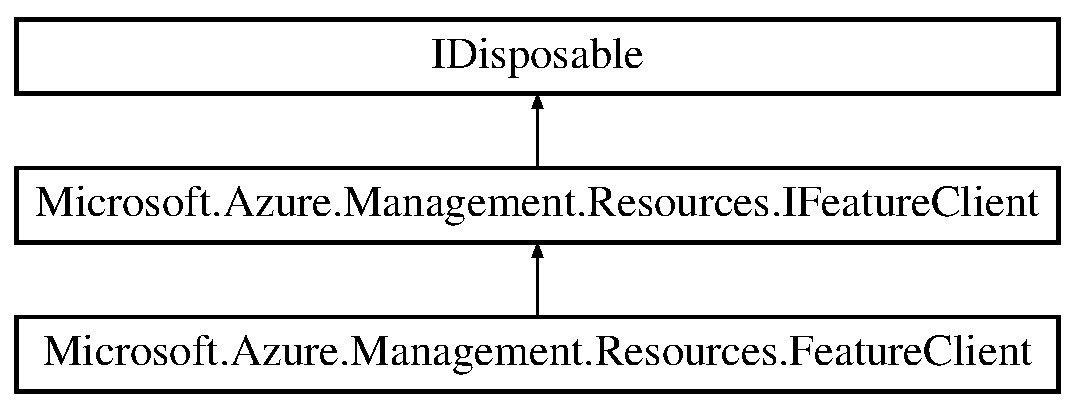
\includegraphics[height=3.000000cm]{interface_microsoft_1_1_azure_1_1_management_1_1_resources_1_1_i_feature_client}
\end{center}
\end{figure}
\subsection*{Properties}
\begin{DoxyCompactItemize}
\item 
Uri \hyperlink{interface_microsoft_1_1_azure_1_1_management_1_1_resources_1_1_i_feature_client_a841253c49ee8275ce3cc3a1a65aa1492}{Base\+Uri}\hspace{0.3cm}{\ttfamily  \mbox{[}get, set\mbox{]}}
\begin{DoxyCompactList}\small\item\em The base U\+RI of the service. \end{DoxyCompactList}\item 
Json\+Serializer\+Settings \hyperlink{interface_microsoft_1_1_azure_1_1_management_1_1_resources_1_1_i_feature_client_a2a98d523ce76fdf9ae319bf310e6a4a9}{Serialization\+Settings}\hspace{0.3cm}{\ttfamily  \mbox{[}get\mbox{]}}
\begin{DoxyCompactList}\small\item\em Gets or sets json serialization settings. \end{DoxyCompactList}\item 
Json\+Serializer\+Settings \hyperlink{interface_microsoft_1_1_azure_1_1_management_1_1_resources_1_1_i_feature_client_a04abe71b204719222477892084ff0577}{Deserialization\+Settings}\hspace{0.3cm}{\ttfamily  \mbox{[}get\mbox{]}}
\begin{DoxyCompactList}\small\item\em Gets or sets json deserialization settings. \end{DoxyCompactList}\item 
Service\+Client\+Credentials \hyperlink{interface_microsoft_1_1_azure_1_1_management_1_1_resources_1_1_i_feature_client_acbfa5924ab9d9871876fb1368c33b523}{Credentials}\hspace{0.3cm}{\ttfamily  \mbox{[}get\mbox{]}}
\begin{DoxyCompactList}\small\item\em The management credentials for \hyperlink{namespace_microsoft_1_1_azure}{Azure}. \end{DoxyCompactList}\item 
string \hyperlink{interface_microsoft_1_1_azure_1_1_management_1_1_resources_1_1_i_feature_client_ac47fd4a6f6356b38a291881ef7f7306f}{Subscription\+Id}\hspace{0.3cm}{\ttfamily  \mbox{[}get, set\mbox{]}}
\begin{DoxyCompactList}\small\item\em Gets subscription credentials which uniquely identify \hyperlink{namespace_microsoft}{Microsoft} \hyperlink{namespace_microsoft_1_1_azure}{Azure} subscription. The subscription ID forms part of the U\+RI for every service call. \end{DoxyCompactList}\item 
string \hyperlink{interface_microsoft_1_1_azure_1_1_management_1_1_resources_1_1_i_feature_client_acec2db4cc82d4ed9b62742987e939b7d}{Api\+Version}\hspace{0.3cm}{\ttfamily  \mbox{[}get\mbox{]}}
\begin{DoxyCompactList}\small\item\em Client Api Version. \end{DoxyCompactList}\item 
string \hyperlink{interface_microsoft_1_1_azure_1_1_management_1_1_resources_1_1_i_feature_client_a7c42e3ad984a1575d7437680b296a7e0}{Accept\+Language}\hspace{0.3cm}{\ttfamily  \mbox{[}get, set\mbox{]}}
\begin{DoxyCompactList}\small\item\em Gets or sets the preferred language for the response. \end{DoxyCompactList}\item 
int \hyperlink{interface_microsoft_1_1_azure_1_1_management_1_1_resources_1_1_i_feature_client_a9839526a6e3654470308e03412425451}{Long\+Running\+Operation\+Retry\+Timeout}\hspace{0.3cm}{\ttfamily  \mbox{[}get, set\mbox{]}}
\begin{DoxyCompactList}\small\item\em The retry timeout for Long Running Operations. \end{DoxyCompactList}\item 
\hyperlink{interface_microsoft_1_1_azure_1_1_management_1_1_resources_1_1_i_features_operations}{I\+Features\+Operations} {\bfseries Features}\hspace{0.3cm}{\ttfamily  \mbox{[}get\mbox{]}}\hypertarget{interface_microsoft_1_1_azure_1_1_management_1_1_resources_1_1_i_feature_client_a9b5dc95ff867b589a4a32a03699dfb8e}{}\label{interface_microsoft_1_1_azure_1_1_management_1_1_resources_1_1_i_feature_client_a9b5dc95ff867b589a4a32a03699dfb8e}

\end{DoxyCompactItemize}


\subsection{Detailed Description}




\subsection{Property Documentation}
\index{Microsoft\+::\+Azure\+::\+Management\+::\+Resources\+::\+I\+Feature\+Client@{Microsoft\+::\+Azure\+::\+Management\+::\+Resources\+::\+I\+Feature\+Client}!Accept\+Language@{Accept\+Language}}
\index{Accept\+Language@{Accept\+Language}!Microsoft\+::\+Azure\+::\+Management\+::\+Resources\+::\+I\+Feature\+Client@{Microsoft\+::\+Azure\+::\+Management\+::\+Resources\+::\+I\+Feature\+Client}}
\subsubsection[{\texorpdfstring{Accept\+Language}{AcceptLanguage}}]{\setlength{\rightskip}{0pt plus 5cm}string Microsoft.\+Azure.\+Management.\+Resources.\+I\+Feature\+Client.\+Accept\+Language\hspace{0.3cm}{\ttfamily [get]}, {\ttfamily [set]}}\hypertarget{interface_microsoft_1_1_azure_1_1_management_1_1_resources_1_1_i_feature_client_a7c42e3ad984a1575d7437680b296a7e0}{}\label{interface_microsoft_1_1_azure_1_1_management_1_1_resources_1_1_i_feature_client_a7c42e3ad984a1575d7437680b296a7e0}


Gets or sets the preferred language for the response. 

\index{Microsoft\+::\+Azure\+::\+Management\+::\+Resources\+::\+I\+Feature\+Client@{Microsoft\+::\+Azure\+::\+Management\+::\+Resources\+::\+I\+Feature\+Client}!Api\+Version@{Api\+Version}}
\index{Api\+Version@{Api\+Version}!Microsoft\+::\+Azure\+::\+Management\+::\+Resources\+::\+I\+Feature\+Client@{Microsoft\+::\+Azure\+::\+Management\+::\+Resources\+::\+I\+Feature\+Client}}
\subsubsection[{\texorpdfstring{Api\+Version}{ApiVersion}}]{\setlength{\rightskip}{0pt plus 5cm}string Microsoft.\+Azure.\+Management.\+Resources.\+I\+Feature\+Client.\+Api\+Version\hspace{0.3cm}{\ttfamily [get]}}\hypertarget{interface_microsoft_1_1_azure_1_1_management_1_1_resources_1_1_i_feature_client_acec2db4cc82d4ed9b62742987e939b7d}{}\label{interface_microsoft_1_1_azure_1_1_management_1_1_resources_1_1_i_feature_client_acec2db4cc82d4ed9b62742987e939b7d}


Client Api Version. 

\index{Microsoft\+::\+Azure\+::\+Management\+::\+Resources\+::\+I\+Feature\+Client@{Microsoft\+::\+Azure\+::\+Management\+::\+Resources\+::\+I\+Feature\+Client}!Base\+Uri@{Base\+Uri}}
\index{Base\+Uri@{Base\+Uri}!Microsoft\+::\+Azure\+::\+Management\+::\+Resources\+::\+I\+Feature\+Client@{Microsoft\+::\+Azure\+::\+Management\+::\+Resources\+::\+I\+Feature\+Client}}
\subsubsection[{\texorpdfstring{Base\+Uri}{BaseUri}}]{\setlength{\rightskip}{0pt plus 5cm}Uri Microsoft.\+Azure.\+Management.\+Resources.\+I\+Feature\+Client.\+Base\+Uri\hspace{0.3cm}{\ttfamily [get]}, {\ttfamily [set]}}\hypertarget{interface_microsoft_1_1_azure_1_1_management_1_1_resources_1_1_i_feature_client_a841253c49ee8275ce3cc3a1a65aa1492}{}\label{interface_microsoft_1_1_azure_1_1_management_1_1_resources_1_1_i_feature_client_a841253c49ee8275ce3cc3a1a65aa1492}


The base U\+RI of the service. 

\index{Microsoft\+::\+Azure\+::\+Management\+::\+Resources\+::\+I\+Feature\+Client@{Microsoft\+::\+Azure\+::\+Management\+::\+Resources\+::\+I\+Feature\+Client}!Credentials@{Credentials}}
\index{Credentials@{Credentials}!Microsoft\+::\+Azure\+::\+Management\+::\+Resources\+::\+I\+Feature\+Client@{Microsoft\+::\+Azure\+::\+Management\+::\+Resources\+::\+I\+Feature\+Client}}
\subsubsection[{\texorpdfstring{Credentials}{Credentials}}]{\setlength{\rightskip}{0pt plus 5cm}Service\+Client\+Credentials Microsoft.\+Azure.\+Management.\+Resources.\+I\+Feature\+Client.\+Credentials\hspace{0.3cm}{\ttfamily [get]}}\hypertarget{interface_microsoft_1_1_azure_1_1_management_1_1_resources_1_1_i_feature_client_acbfa5924ab9d9871876fb1368c33b523}{}\label{interface_microsoft_1_1_azure_1_1_management_1_1_resources_1_1_i_feature_client_acbfa5924ab9d9871876fb1368c33b523}


The management credentials for \hyperlink{namespace_microsoft_1_1_azure}{Azure}. 

\index{Microsoft\+::\+Azure\+::\+Management\+::\+Resources\+::\+I\+Feature\+Client@{Microsoft\+::\+Azure\+::\+Management\+::\+Resources\+::\+I\+Feature\+Client}!Deserialization\+Settings@{Deserialization\+Settings}}
\index{Deserialization\+Settings@{Deserialization\+Settings}!Microsoft\+::\+Azure\+::\+Management\+::\+Resources\+::\+I\+Feature\+Client@{Microsoft\+::\+Azure\+::\+Management\+::\+Resources\+::\+I\+Feature\+Client}}
\subsubsection[{\texorpdfstring{Deserialization\+Settings}{DeserializationSettings}}]{\setlength{\rightskip}{0pt plus 5cm}Json\+Serializer\+Settings Microsoft.\+Azure.\+Management.\+Resources.\+I\+Feature\+Client.\+Deserialization\+Settings\hspace{0.3cm}{\ttfamily [get]}}\hypertarget{interface_microsoft_1_1_azure_1_1_management_1_1_resources_1_1_i_feature_client_a04abe71b204719222477892084ff0577}{}\label{interface_microsoft_1_1_azure_1_1_management_1_1_resources_1_1_i_feature_client_a04abe71b204719222477892084ff0577}


Gets or sets json deserialization settings. 

\index{Microsoft\+::\+Azure\+::\+Management\+::\+Resources\+::\+I\+Feature\+Client@{Microsoft\+::\+Azure\+::\+Management\+::\+Resources\+::\+I\+Feature\+Client}!Long\+Running\+Operation\+Retry\+Timeout@{Long\+Running\+Operation\+Retry\+Timeout}}
\index{Long\+Running\+Operation\+Retry\+Timeout@{Long\+Running\+Operation\+Retry\+Timeout}!Microsoft\+::\+Azure\+::\+Management\+::\+Resources\+::\+I\+Feature\+Client@{Microsoft\+::\+Azure\+::\+Management\+::\+Resources\+::\+I\+Feature\+Client}}
\subsubsection[{\texorpdfstring{Long\+Running\+Operation\+Retry\+Timeout}{LongRunningOperationRetryTimeout}}]{\setlength{\rightskip}{0pt plus 5cm}int Microsoft.\+Azure.\+Management.\+Resources.\+I\+Feature\+Client.\+Long\+Running\+Operation\+Retry\+Timeout\hspace{0.3cm}{\ttfamily [get]}, {\ttfamily [set]}}\hypertarget{interface_microsoft_1_1_azure_1_1_management_1_1_resources_1_1_i_feature_client_a9839526a6e3654470308e03412425451}{}\label{interface_microsoft_1_1_azure_1_1_management_1_1_resources_1_1_i_feature_client_a9839526a6e3654470308e03412425451}


The retry timeout for Long Running Operations. 

\index{Microsoft\+::\+Azure\+::\+Management\+::\+Resources\+::\+I\+Feature\+Client@{Microsoft\+::\+Azure\+::\+Management\+::\+Resources\+::\+I\+Feature\+Client}!Serialization\+Settings@{Serialization\+Settings}}
\index{Serialization\+Settings@{Serialization\+Settings}!Microsoft\+::\+Azure\+::\+Management\+::\+Resources\+::\+I\+Feature\+Client@{Microsoft\+::\+Azure\+::\+Management\+::\+Resources\+::\+I\+Feature\+Client}}
\subsubsection[{\texorpdfstring{Serialization\+Settings}{SerializationSettings}}]{\setlength{\rightskip}{0pt plus 5cm}Json\+Serializer\+Settings Microsoft.\+Azure.\+Management.\+Resources.\+I\+Feature\+Client.\+Serialization\+Settings\hspace{0.3cm}{\ttfamily [get]}}\hypertarget{interface_microsoft_1_1_azure_1_1_management_1_1_resources_1_1_i_feature_client_a2a98d523ce76fdf9ae319bf310e6a4a9}{}\label{interface_microsoft_1_1_azure_1_1_management_1_1_resources_1_1_i_feature_client_a2a98d523ce76fdf9ae319bf310e6a4a9}


Gets or sets json serialization settings. 

\index{Microsoft\+::\+Azure\+::\+Management\+::\+Resources\+::\+I\+Feature\+Client@{Microsoft\+::\+Azure\+::\+Management\+::\+Resources\+::\+I\+Feature\+Client}!Subscription\+Id@{Subscription\+Id}}
\index{Subscription\+Id@{Subscription\+Id}!Microsoft\+::\+Azure\+::\+Management\+::\+Resources\+::\+I\+Feature\+Client@{Microsoft\+::\+Azure\+::\+Management\+::\+Resources\+::\+I\+Feature\+Client}}
\subsubsection[{\texorpdfstring{Subscription\+Id}{SubscriptionId}}]{\setlength{\rightskip}{0pt plus 5cm}string Microsoft.\+Azure.\+Management.\+Resources.\+I\+Feature\+Client.\+Subscription\+Id\hspace{0.3cm}{\ttfamily [get]}, {\ttfamily [set]}}\hypertarget{interface_microsoft_1_1_azure_1_1_management_1_1_resources_1_1_i_feature_client_ac47fd4a6f6356b38a291881ef7f7306f}{}\label{interface_microsoft_1_1_azure_1_1_management_1_1_resources_1_1_i_feature_client_ac47fd4a6f6356b38a291881ef7f7306f}


Gets subscription credentials which uniquely identify \hyperlink{namespace_microsoft}{Microsoft} \hyperlink{namespace_microsoft_1_1_azure}{Azure} subscription. The subscription ID forms part of the U\+RI for every service call. 



The documentation for this interface was generated from the following file\+:\begin{DoxyCompactItemize}
\item 
files/I\+Feature\+Client.\+cs\end{DoxyCompactItemize}

\hypertarget{interface_microsoft_1_1_azure_1_1_management_1_1_resources_1_1_i_features_operations}{}\section{Microsoft.\+Azure.\+Management.\+Resources.\+I\+Features\+Operations Interface Reference}
\label{interface_microsoft_1_1_azure_1_1_management_1_1_resources_1_1_i_features_operations}\index{Microsoft.\+Azure.\+Management.\+Resources.\+I\+Features\+Operations@{Microsoft.\+Azure.\+Management.\+Resources.\+I\+Features\+Operations}}


Features\+Operations operations.  




Inherited by Microsoft.\+Azure.\+Management.\+Resources.\+Features\+Operations.

\subsection*{Public Member Functions}
\begin{DoxyCompactItemize}
\item 
Task$<$ Azure\+Operation\+Response$<$ I\+Page$<$ Feature\+Result $>$ $>$ $>$ \hyperlink{interface_microsoft_1_1_azure_1_1_management_1_1_resources_1_1_i_features_operations_a163a1fcd16988193898bcc3131ac0ee0}{List\+All\+With\+Http\+Messages\+Async} (Dictionary$<$ string, List$<$ string $>$$>$ custom\+Headers=null, Cancellation\+Token cancellation\+Token=default(Cancellation\+Token))
\begin{DoxyCompactList}\small\item\em Gets a list of previewed features for all the providers in the current subscription. \end{DoxyCompactList}\item 
Task$<$ Azure\+Operation\+Response$<$ I\+Page$<$ Feature\+Result $>$ $>$ $>$ \hyperlink{interface_microsoft_1_1_azure_1_1_management_1_1_resources_1_1_i_features_operations_a5fb7a48877eaa1481a45dbc03238ce7c}{List\+With\+Http\+Messages\+Async} (string resource\+Provider\+Namespace, Dictionary$<$ string, List$<$ string $>$$>$ custom\+Headers=null, Cancellation\+Token cancellation\+Token=default(Cancellation\+Token))
\begin{DoxyCompactList}\small\item\em Gets a list of previewed features of a resource provider. \end{DoxyCompactList}\item 
Task$<$ Azure\+Operation\+Response$<$ Feature\+Result $>$ $>$ \hyperlink{interface_microsoft_1_1_azure_1_1_management_1_1_resources_1_1_i_features_operations_a46c7219d2e7638da350f40371a79a8ca}{Get\+With\+Http\+Messages\+Async} (string resource\+Provider\+Namespace, string feature\+Name, Dictionary$<$ string, List$<$ string $>$$>$ custom\+Headers=null, Cancellation\+Token cancellation\+Token=default(Cancellation\+Token))
\begin{DoxyCompactList}\small\item\em Get all features under the subscription. \end{DoxyCompactList}\item 
Task$<$ Azure\+Operation\+Response$<$ Feature\+Result $>$ $>$ \hyperlink{interface_microsoft_1_1_azure_1_1_management_1_1_resources_1_1_i_features_operations_ae4e6eaf03a6f94b0821f80d9d9a99eaf}{Register\+With\+Http\+Messages\+Async} (string resource\+Provider\+Namespace, string feature\+Name, Dictionary$<$ string, List$<$ string $>$$>$ custom\+Headers=null, Cancellation\+Token cancellation\+Token=default(Cancellation\+Token))
\begin{DoxyCompactList}\small\item\em Registers for a previewed feature of a resource provider. \end{DoxyCompactList}\item 
Task$<$ Azure\+Operation\+Response$<$ I\+Page$<$ Feature\+Result $>$ $>$ $>$ \hyperlink{interface_microsoft_1_1_azure_1_1_management_1_1_resources_1_1_i_features_operations_aaebc2d4dceec07e27b1784dbdb4ad764}{List\+All\+Next\+With\+Http\+Messages\+Async} (string next\+Page\+Link, Dictionary$<$ string, List$<$ string $>$$>$ custom\+Headers=null, Cancellation\+Token cancellation\+Token=default(Cancellation\+Token))
\begin{DoxyCompactList}\small\item\em Gets a list of previewed features for all the providers in the current subscription. \end{DoxyCompactList}\item 
Task$<$ Azure\+Operation\+Response$<$ I\+Page$<$ Feature\+Result $>$ $>$ $>$ \hyperlink{interface_microsoft_1_1_azure_1_1_management_1_1_resources_1_1_i_features_operations_a167272af669ce6388a7c278b7d58d6f7}{List\+Next\+With\+Http\+Messages\+Async} (string next\+Page\+Link, Dictionary$<$ string, List$<$ string $>$$>$ custom\+Headers=null, Cancellation\+Token cancellation\+Token=default(Cancellation\+Token))
\begin{DoxyCompactList}\small\item\em Gets a list of previewed features of a resource provider. \end{DoxyCompactList}\end{DoxyCompactItemize}


\subsection{Detailed Description}
Features\+Operations operations. 



\subsection{Member Function Documentation}
\index{Microsoft\+::\+Azure\+::\+Management\+::\+Resources\+::\+I\+Features\+Operations@{Microsoft\+::\+Azure\+::\+Management\+::\+Resources\+::\+I\+Features\+Operations}!Get\+With\+Http\+Messages\+Async@{Get\+With\+Http\+Messages\+Async}}
\index{Get\+With\+Http\+Messages\+Async@{Get\+With\+Http\+Messages\+Async}!Microsoft\+::\+Azure\+::\+Management\+::\+Resources\+::\+I\+Features\+Operations@{Microsoft\+::\+Azure\+::\+Management\+::\+Resources\+::\+I\+Features\+Operations}}
\subsubsection[{\texorpdfstring{Get\+With\+Http\+Messages\+Async(string resource\+Provider\+Namespace, string feature\+Name, Dictionary$<$ string, List$<$ string $>$$>$ custom\+Headers=null, Cancellation\+Token cancellation\+Token=default(\+Cancellation\+Token))}{GetWithHttpMessagesAsync(string resourceProviderNamespace, string featureName, Dictionary< string, List< string >> customHeaders=null, CancellationToken cancellationToken=default(CancellationToken))}}]{\setlength{\rightskip}{0pt plus 5cm}Task$<$Azure\+Operation\+Response$<$Feature\+Result$>$ $>$ Microsoft.\+Azure.\+Management.\+Resources.\+I\+Features\+Operations.\+Get\+With\+Http\+Messages\+Async (
\begin{DoxyParamCaption}
\item[{string}]{resource\+Provider\+Namespace, }
\item[{string}]{feature\+Name, }
\item[{Dictionary$<$ string, List$<$ string $>$$>$}]{custom\+Headers = {\ttfamily null}, }
\item[{Cancellation\+Token}]{cancellation\+Token = {\ttfamily default(CancellationToken)}}
\end{DoxyParamCaption}
)}\hypertarget{interface_microsoft_1_1_azure_1_1_management_1_1_resources_1_1_i_features_operations_a46c7219d2e7638da350f40371a79a8ca}{}\label{interface_microsoft_1_1_azure_1_1_management_1_1_resources_1_1_i_features_operations_a46c7219d2e7638da350f40371a79a8ca}


Get all features under the subscription. 


\begin{DoxyParams}{Parameters}
{\em resource\+Provider\+Namespace} & Namespace of the resource provider. \\
\hline
{\em feature\+Name} & Previewed feature name in the resource provider. \\
\hline
{\em custom\+Headers} & The headers that will be added to request. \\
\hline
{\em cancellation\+Token} & The cancellation token. \\
\hline
\end{DoxyParams}
\index{Microsoft\+::\+Azure\+::\+Management\+::\+Resources\+::\+I\+Features\+Operations@{Microsoft\+::\+Azure\+::\+Management\+::\+Resources\+::\+I\+Features\+Operations}!List\+All\+Next\+With\+Http\+Messages\+Async@{List\+All\+Next\+With\+Http\+Messages\+Async}}
\index{List\+All\+Next\+With\+Http\+Messages\+Async@{List\+All\+Next\+With\+Http\+Messages\+Async}!Microsoft\+::\+Azure\+::\+Management\+::\+Resources\+::\+I\+Features\+Operations@{Microsoft\+::\+Azure\+::\+Management\+::\+Resources\+::\+I\+Features\+Operations}}
\subsubsection[{\texorpdfstring{List\+All\+Next\+With\+Http\+Messages\+Async(string next\+Page\+Link, Dictionary$<$ string, List$<$ string $>$$>$ custom\+Headers=null, Cancellation\+Token cancellation\+Token=default(\+Cancellation\+Token))}{ListAllNextWithHttpMessagesAsync(string nextPageLink, Dictionary< string, List< string >> customHeaders=null, CancellationToken cancellationToken=default(CancellationToken))}}]{\setlength{\rightskip}{0pt plus 5cm}Task$<$Azure\+Operation\+Response$<$I\+Page$<$Feature\+Result$>$ $>$ $>$ Microsoft.\+Azure.\+Management.\+Resources.\+I\+Features\+Operations.\+List\+All\+Next\+With\+Http\+Messages\+Async (
\begin{DoxyParamCaption}
\item[{string}]{next\+Page\+Link, }
\item[{Dictionary$<$ string, List$<$ string $>$$>$}]{custom\+Headers = {\ttfamily null}, }
\item[{Cancellation\+Token}]{cancellation\+Token = {\ttfamily default(CancellationToken)}}
\end{DoxyParamCaption}
)}\hypertarget{interface_microsoft_1_1_azure_1_1_management_1_1_resources_1_1_i_features_operations_aaebc2d4dceec07e27b1784dbdb4ad764}{}\label{interface_microsoft_1_1_azure_1_1_management_1_1_resources_1_1_i_features_operations_aaebc2d4dceec07e27b1784dbdb4ad764}


Gets a list of previewed features for all the providers in the current subscription. 


\begin{DoxyParams}{Parameters}
{\em next\+Page\+Link} & The Next\+Link from the previous successful call to List operation. \\
\hline
{\em custom\+Headers} & The headers that will be added to request. \\
\hline
{\em cancellation\+Token} & The cancellation token. \\
\hline
\end{DoxyParams}
\index{Microsoft\+::\+Azure\+::\+Management\+::\+Resources\+::\+I\+Features\+Operations@{Microsoft\+::\+Azure\+::\+Management\+::\+Resources\+::\+I\+Features\+Operations}!List\+All\+With\+Http\+Messages\+Async@{List\+All\+With\+Http\+Messages\+Async}}
\index{List\+All\+With\+Http\+Messages\+Async@{List\+All\+With\+Http\+Messages\+Async}!Microsoft\+::\+Azure\+::\+Management\+::\+Resources\+::\+I\+Features\+Operations@{Microsoft\+::\+Azure\+::\+Management\+::\+Resources\+::\+I\+Features\+Operations}}
\subsubsection[{\texorpdfstring{List\+All\+With\+Http\+Messages\+Async(\+Dictionary$<$ string, List$<$ string $>$$>$ custom\+Headers=null, Cancellation\+Token cancellation\+Token=default(\+Cancellation\+Token))}{ListAllWithHttpMessagesAsync(Dictionary< string, List< string >> customHeaders=null, CancellationToken cancellationToken=default(CancellationToken))}}]{\setlength{\rightskip}{0pt plus 5cm}Task$<$Azure\+Operation\+Response$<$I\+Page$<$Feature\+Result$>$ $>$ $>$ Microsoft.\+Azure.\+Management.\+Resources.\+I\+Features\+Operations.\+List\+All\+With\+Http\+Messages\+Async (
\begin{DoxyParamCaption}
\item[{Dictionary$<$ string, List$<$ string $>$$>$}]{custom\+Headers = {\ttfamily null}, }
\item[{Cancellation\+Token}]{cancellation\+Token = {\ttfamily default(CancellationToken)}}
\end{DoxyParamCaption}
)}\hypertarget{interface_microsoft_1_1_azure_1_1_management_1_1_resources_1_1_i_features_operations_a163a1fcd16988193898bcc3131ac0ee0}{}\label{interface_microsoft_1_1_azure_1_1_management_1_1_resources_1_1_i_features_operations_a163a1fcd16988193898bcc3131ac0ee0}


Gets a list of previewed features for all the providers in the current subscription. 


\begin{DoxyParams}{Parameters}
{\em custom\+Headers} & The headers that will be added to request. \\
\hline
{\em cancellation\+Token} & The cancellation token. \\
\hline
\end{DoxyParams}
\index{Microsoft\+::\+Azure\+::\+Management\+::\+Resources\+::\+I\+Features\+Operations@{Microsoft\+::\+Azure\+::\+Management\+::\+Resources\+::\+I\+Features\+Operations}!List\+Next\+With\+Http\+Messages\+Async@{List\+Next\+With\+Http\+Messages\+Async}}
\index{List\+Next\+With\+Http\+Messages\+Async@{List\+Next\+With\+Http\+Messages\+Async}!Microsoft\+::\+Azure\+::\+Management\+::\+Resources\+::\+I\+Features\+Operations@{Microsoft\+::\+Azure\+::\+Management\+::\+Resources\+::\+I\+Features\+Operations}}
\subsubsection[{\texorpdfstring{List\+Next\+With\+Http\+Messages\+Async(string next\+Page\+Link, Dictionary$<$ string, List$<$ string $>$$>$ custom\+Headers=null, Cancellation\+Token cancellation\+Token=default(\+Cancellation\+Token))}{ListNextWithHttpMessagesAsync(string nextPageLink, Dictionary< string, List< string >> customHeaders=null, CancellationToken cancellationToken=default(CancellationToken))}}]{\setlength{\rightskip}{0pt plus 5cm}Task$<$Azure\+Operation\+Response$<$I\+Page$<$Feature\+Result$>$ $>$ $>$ Microsoft.\+Azure.\+Management.\+Resources.\+I\+Features\+Operations.\+List\+Next\+With\+Http\+Messages\+Async (
\begin{DoxyParamCaption}
\item[{string}]{next\+Page\+Link, }
\item[{Dictionary$<$ string, List$<$ string $>$$>$}]{custom\+Headers = {\ttfamily null}, }
\item[{Cancellation\+Token}]{cancellation\+Token = {\ttfamily default(CancellationToken)}}
\end{DoxyParamCaption}
)}\hypertarget{interface_microsoft_1_1_azure_1_1_management_1_1_resources_1_1_i_features_operations_a167272af669ce6388a7c278b7d58d6f7}{}\label{interface_microsoft_1_1_azure_1_1_management_1_1_resources_1_1_i_features_operations_a167272af669ce6388a7c278b7d58d6f7}


Gets a list of previewed features of a resource provider. 


\begin{DoxyParams}{Parameters}
{\em next\+Page\+Link} & The Next\+Link from the previous successful call to List operation. \\
\hline
{\em custom\+Headers} & The headers that will be added to request. \\
\hline
{\em cancellation\+Token} & The cancellation token. \\
\hline
\end{DoxyParams}
\index{Microsoft\+::\+Azure\+::\+Management\+::\+Resources\+::\+I\+Features\+Operations@{Microsoft\+::\+Azure\+::\+Management\+::\+Resources\+::\+I\+Features\+Operations}!List\+With\+Http\+Messages\+Async@{List\+With\+Http\+Messages\+Async}}
\index{List\+With\+Http\+Messages\+Async@{List\+With\+Http\+Messages\+Async}!Microsoft\+::\+Azure\+::\+Management\+::\+Resources\+::\+I\+Features\+Operations@{Microsoft\+::\+Azure\+::\+Management\+::\+Resources\+::\+I\+Features\+Operations}}
\subsubsection[{\texorpdfstring{List\+With\+Http\+Messages\+Async(string resource\+Provider\+Namespace, Dictionary$<$ string, List$<$ string $>$$>$ custom\+Headers=null, Cancellation\+Token cancellation\+Token=default(\+Cancellation\+Token))}{ListWithHttpMessagesAsync(string resourceProviderNamespace, Dictionary< string, List< string >> customHeaders=null, CancellationToken cancellationToken=default(CancellationToken))}}]{\setlength{\rightskip}{0pt plus 5cm}Task$<$Azure\+Operation\+Response$<$I\+Page$<$Feature\+Result$>$ $>$ $>$ Microsoft.\+Azure.\+Management.\+Resources.\+I\+Features\+Operations.\+List\+With\+Http\+Messages\+Async (
\begin{DoxyParamCaption}
\item[{string}]{resource\+Provider\+Namespace, }
\item[{Dictionary$<$ string, List$<$ string $>$$>$}]{custom\+Headers = {\ttfamily null}, }
\item[{Cancellation\+Token}]{cancellation\+Token = {\ttfamily default(CancellationToken)}}
\end{DoxyParamCaption}
)}\hypertarget{interface_microsoft_1_1_azure_1_1_management_1_1_resources_1_1_i_features_operations_a5fb7a48877eaa1481a45dbc03238ce7c}{}\label{interface_microsoft_1_1_azure_1_1_management_1_1_resources_1_1_i_features_operations_a5fb7a48877eaa1481a45dbc03238ce7c}


Gets a list of previewed features of a resource provider. 


\begin{DoxyParams}{Parameters}
{\em resource\+Provider\+Namespace} & The namespace of the resource provider. \\
\hline
{\em custom\+Headers} & The headers that will be added to request. \\
\hline
{\em cancellation\+Token} & The cancellation token. \\
\hline
\end{DoxyParams}
\index{Microsoft\+::\+Azure\+::\+Management\+::\+Resources\+::\+I\+Features\+Operations@{Microsoft\+::\+Azure\+::\+Management\+::\+Resources\+::\+I\+Features\+Operations}!Register\+With\+Http\+Messages\+Async@{Register\+With\+Http\+Messages\+Async}}
\index{Register\+With\+Http\+Messages\+Async@{Register\+With\+Http\+Messages\+Async}!Microsoft\+::\+Azure\+::\+Management\+::\+Resources\+::\+I\+Features\+Operations@{Microsoft\+::\+Azure\+::\+Management\+::\+Resources\+::\+I\+Features\+Operations}}
\subsubsection[{\texorpdfstring{Register\+With\+Http\+Messages\+Async(string resource\+Provider\+Namespace, string feature\+Name, Dictionary$<$ string, List$<$ string $>$$>$ custom\+Headers=null, Cancellation\+Token cancellation\+Token=default(\+Cancellation\+Token))}{RegisterWithHttpMessagesAsync(string resourceProviderNamespace, string featureName, Dictionary< string, List< string >> customHeaders=null, CancellationToken cancellationToken=default(CancellationToken))}}]{\setlength{\rightskip}{0pt plus 5cm}Task$<$Azure\+Operation\+Response$<$Feature\+Result$>$ $>$ Microsoft.\+Azure.\+Management.\+Resources.\+I\+Features\+Operations.\+Register\+With\+Http\+Messages\+Async (
\begin{DoxyParamCaption}
\item[{string}]{resource\+Provider\+Namespace, }
\item[{string}]{feature\+Name, }
\item[{Dictionary$<$ string, List$<$ string $>$$>$}]{custom\+Headers = {\ttfamily null}, }
\item[{Cancellation\+Token}]{cancellation\+Token = {\ttfamily default(CancellationToken)}}
\end{DoxyParamCaption}
)}\hypertarget{interface_microsoft_1_1_azure_1_1_management_1_1_resources_1_1_i_features_operations_ae4e6eaf03a6f94b0821f80d9d9a99eaf}{}\label{interface_microsoft_1_1_azure_1_1_management_1_1_resources_1_1_i_features_operations_ae4e6eaf03a6f94b0821f80d9d9a99eaf}


Registers for a previewed feature of a resource provider. 


\begin{DoxyParams}{Parameters}
{\em resource\+Provider\+Namespace} & Namespace of the resource provider. \\
\hline
{\em feature\+Name} & Previewed feature name in the resource provider. \\
\hline
{\em custom\+Headers} & The headers that will be added to request. \\
\hline
{\em cancellation\+Token} & The cancellation token. \\
\hline
\end{DoxyParams}


The documentation for this interface was generated from the following file\+:\begin{DoxyCompactItemize}
\item 
files/I\+Features\+Operations.\+cs\end{DoxyCompactItemize}

\hypertarget{interface_microsoft_1_1_azure_1_1_management_1_1_resources_1_1_i_management_locks_operations}{}\section{Microsoft.\+Azure.\+Management.\+Resources.\+I\+Management\+Locks\+Operations Interface Reference}
\label{interface_microsoft_1_1_azure_1_1_management_1_1_resources_1_1_i_management_locks_operations}\index{Microsoft.\+Azure.\+Management.\+Resources.\+I\+Management\+Locks\+Operations@{Microsoft.\+Azure.\+Management.\+Resources.\+I\+Management\+Locks\+Operations}}


Management\+Locks\+Operations operations.  




Inherited by Microsoft.\+Azure.\+Management.\+Resources.\+Management\+Locks\+Operations.

\subsection*{Public Member Functions}
\begin{DoxyCompactItemize}
\item 
Task$<$ Azure\+Operation\+Response$<$ Management\+Lock\+Object $>$ $>$ \hyperlink{interface_microsoft_1_1_azure_1_1_management_1_1_resources_1_1_i_management_locks_operations_a0416dc292db36776c1b4786d80074b7d}{Create\+Or\+Update\+At\+Resource\+Group\+Level\+With\+Http\+Messages\+Async} (string resource\+Group\+Name, string lock\+Name, Management\+Lock\+Object parameters, Dictionary$<$ string, List$<$ string $>$$>$ custom\+Headers=null, Cancellation\+Token cancellation\+Token=default(Cancellation\+Token))
\begin{DoxyCompactList}\small\item\em Create or update a management lock at the resource group level. \end{DoxyCompactList}\item 
Task$<$ Azure\+Operation\+Response$<$ Management\+Lock\+Object $>$ $>$ \hyperlink{interface_microsoft_1_1_azure_1_1_management_1_1_resources_1_1_i_management_locks_operations_a11677d16f93b691d53113375e49c5abd}{Create\+Or\+Update\+At\+Resource\+Level\+With\+Http\+Messages\+Async} (string resource\+Group\+Name, string resource\+Provider\+Namespace, string parent\+Resource\+Path, string resource\+Type, string resource\+Name, string lock\+Name, Management\+Lock\+Object parameters, Dictionary$<$ string, List$<$ string $>$$>$ custom\+Headers=null, Cancellation\+Token cancellation\+Token=default(Cancellation\+Token))
\begin{DoxyCompactList}\small\item\em Create or update a management lock at the resource level or any level below resource. \end{DoxyCompactList}\item 
Task$<$ Azure\+Operation\+Response $>$ \hyperlink{interface_microsoft_1_1_azure_1_1_management_1_1_resources_1_1_i_management_locks_operations_a1a680da1a4835d38e1b4058c93f949fa}{Delete\+At\+Resource\+Level\+With\+Http\+Messages\+Async} (string resource\+Group\+Name, string resource\+Provider\+Namespace, string parent\+Resource\+Path, string resource\+Type, string resource\+Name, string lock\+Name, Dictionary$<$ string, List$<$ string $>$$>$ custom\+Headers=null, Cancellation\+Token cancellation\+Token=default(Cancellation\+Token))
\begin{DoxyCompactList}\small\item\em Deletes the management lock of a resource or any level below resource. \end{DoxyCompactList}\item 
Task$<$ Azure\+Operation\+Response$<$ Management\+Lock\+Object $>$ $>$ \hyperlink{interface_microsoft_1_1_azure_1_1_management_1_1_resources_1_1_i_management_locks_operations_a58f67611b100e0ece138e1d9ebaa206c}{Create\+Or\+Update\+At\+Subscription\+Level\+With\+Http\+Messages\+Async} (string lock\+Name, Management\+Lock\+Object parameters, Dictionary$<$ string, List$<$ string $>$$>$ custom\+Headers=null, Cancellation\+Token cancellation\+Token=default(Cancellation\+Token))
\begin{DoxyCompactList}\small\item\em Create or update a management lock at the subscription level. \end{DoxyCompactList}\item 
Task$<$ Azure\+Operation\+Response $>$ \hyperlink{interface_microsoft_1_1_azure_1_1_management_1_1_resources_1_1_i_management_locks_operations_a6a7f8089bce87a447873131e274cbdeb}{Delete\+At\+Subscription\+Level\+With\+Http\+Messages\+Async} (string lock\+Name, Dictionary$<$ string, List$<$ string $>$$>$ custom\+Headers=null, Cancellation\+Token cancellation\+Token=default(Cancellation\+Token))
\begin{DoxyCompactList}\small\item\em Deletes the management lock of a subscription. \end{DoxyCompactList}\item 
Task$<$ Azure\+Operation\+Response$<$ Management\+Lock\+Object $>$ $>$ \hyperlink{interface_microsoft_1_1_azure_1_1_management_1_1_resources_1_1_i_management_locks_operations_a7fe872ce8132bf9ad4d658c32f7b6fd5}{Get\+With\+Http\+Messages\+Async} (string lock\+Name, Dictionary$<$ string, List$<$ string $>$$>$ custom\+Headers=null, Cancellation\+Token cancellation\+Token=default(Cancellation\+Token))
\begin{DoxyCompactList}\small\item\em Gets the management lock of a scope. \end{DoxyCompactList}\item 
Task$<$ Azure\+Operation\+Response $>$ \hyperlink{interface_microsoft_1_1_azure_1_1_management_1_1_resources_1_1_i_management_locks_operations_ab6a3b62add2d30fbf069899dcfd09b51}{Delete\+At\+Resource\+Group\+Level\+With\+Http\+Messages\+Async} (string resource\+Group, string lock\+Name, Dictionary$<$ string, List$<$ string $>$$>$ custom\+Headers=null, Cancellation\+Token cancellation\+Token=default(Cancellation\+Token))
\begin{DoxyCompactList}\small\item\em Deletes the management lock of a resource group. \end{DoxyCompactList}\item 
Task$<$ Azure\+Operation\+Response$<$ I\+Page$<$ Management\+Lock\+Object $>$ $>$ $>$ \hyperlink{interface_microsoft_1_1_azure_1_1_management_1_1_resources_1_1_i_management_locks_operations_abf108939936818afb2f7f2bf250cdc96}{List\+At\+Resource\+Group\+Level\+With\+Http\+Messages\+Async} (string resource\+Group\+Name, O\+Data\+Query$<$ Management\+Lock\+Object $>$ odata\+Query=default(O\+Data\+Query$<$ Management\+Lock\+Object $>$), Dictionary$<$ string, List$<$ string $>$$>$ custom\+Headers=null, Cancellation\+Token cancellation\+Token=default(Cancellation\+Token))
\begin{DoxyCompactList}\small\item\em Gets all the management locks of a resource group. \end{DoxyCompactList}\item 
Task$<$ Azure\+Operation\+Response$<$ I\+Page$<$ Management\+Lock\+Object $>$ $>$ $>$ \hyperlink{interface_microsoft_1_1_azure_1_1_management_1_1_resources_1_1_i_management_locks_operations_a23a684c365fafb8082c1a4b8a97a21a7}{List\+At\+Resource\+Level\+With\+Http\+Messages\+Async} (string resource\+Group\+Name, string resource\+Provider\+Namespace, string parent\+Resource\+Path, string resource\+Type, string resource\+Name, O\+Data\+Query$<$ Management\+Lock\+Object $>$ odata\+Query=default(O\+Data\+Query$<$ Management\+Lock\+Object $>$), Dictionary$<$ string, List$<$ string $>$$>$ custom\+Headers=null, Cancellation\+Token cancellation\+Token=default(Cancellation\+Token))
\begin{DoxyCompactList}\small\item\em Gets all the management locks of a resource or any level below resource. \end{DoxyCompactList}\item 
Task$<$ Azure\+Operation\+Response$<$ I\+Page$<$ Management\+Lock\+Object $>$ $>$ $>$ \hyperlink{interface_microsoft_1_1_azure_1_1_management_1_1_resources_1_1_i_management_locks_operations_a618a29b67ef59ea153ab6b298d43c1c3}{List\+Next\+With\+Http\+Messages\+Async} (string next\+Link, Dictionary$<$ string, List$<$ string $>$$>$ custom\+Headers=null, Cancellation\+Token cancellation\+Token=default(Cancellation\+Token))
\begin{DoxyCompactList}\small\item\em Get a list of management locks at resource level or below. \end{DoxyCompactList}\item 
Task$<$ Azure\+Operation\+Response$<$ I\+Page$<$ Management\+Lock\+Object $>$ $>$ $>$ \hyperlink{interface_microsoft_1_1_azure_1_1_management_1_1_resources_1_1_i_management_locks_operations_a92fa97a75b87a295d9b3a78551edc31e}{List\+At\+Subscription\+Level\+With\+Http\+Messages\+Async} (O\+Data\+Query$<$ Management\+Lock\+Object $>$ odata\+Query=default(O\+Data\+Query$<$ Management\+Lock\+Object $>$), Dictionary$<$ string, List$<$ string $>$$>$ custom\+Headers=null, Cancellation\+Token cancellation\+Token=default(Cancellation\+Token))
\begin{DoxyCompactList}\small\item\em Gets all the management locks of a subscription. \end{DoxyCompactList}\item 
Task$<$ Azure\+Operation\+Response$<$ I\+Page$<$ Management\+Lock\+Object $>$ $>$ $>$ \hyperlink{interface_microsoft_1_1_azure_1_1_management_1_1_resources_1_1_i_management_locks_operations_a80fe1fe9623cf9b544f953604cc3191e}{List\+At\+Resource\+Group\+Level\+Next\+With\+Http\+Messages\+Async} (string next\+Page\+Link, Dictionary$<$ string, List$<$ string $>$$>$ custom\+Headers=null, Cancellation\+Token cancellation\+Token=default(Cancellation\+Token))
\begin{DoxyCompactList}\small\item\em Gets all the management locks of a resource group. \end{DoxyCompactList}\item 
Task$<$ Azure\+Operation\+Response$<$ I\+Page$<$ Management\+Lock\+Object $>$ $>$ $>$ \hyperlink{interface_microsoft_1_1_azure_1_1_management_1_1_resources_1_1_i_management_locks_operations_a248a1c30feca8f07eb6886a5c1370814}{List\+At\+Resource\+Level\+Next\+With\+Http\+Messages\+Async} (string next\+Page\+Link, Dictionary$<$ string, List$<$ string $>$$>$ custom\+Headers=null, Cancellation\+Token cancellation\+Token=default(Cancellation\+Token))
\begin{DoxyCompactList}\small\item\em Gets all the management locks of a resource or any level below resource. \end{DoxyCompactList}\item 
Task$<$ Azure\+Operation\+Response$<$ I\+Page$<$ Management\+Lock\+Object $>$ $>$ $>$ \hyperlink{interface_microsoft_1_1_azure_1_1_management_1_1_resources_1_1_i_management_locks_operations_afb9fc9c291a9a64898362a4adbbde46e}{List\+Next\+Next\+With\+Http\+Messages\+Async} (string next\+Page\+Link, Dictionary$<$ string, List$<$ string $>$$>$ custom\+Headers=null, Cancellation\+Token cancellation\+Token=default(Cancellation\+Token))
\begin{DoxyCompactList}\small\item\em Get a list of management locks at resource level or below. \end{DoxyCompactList}\item 
Task$<$ Azure\+Operation\+Response$<$ I\+Page$<$ Management\+Lock\+Object $>$ $>$ $>$ \hyperlink{interface_microsoft_1_1_azure_1_1_management_1_1_resources_1_1_i_management_locks_operations_a6444be3ad9fd2a67fa952d4cb18f7ccc}{List\+At\+Subscription\+Level\+Next\+With\+Http\+Messages\+Async} (string next\+Page\+Link, Dictionary$<$ string, List$<$ string $>$$>$ custom\+Headers=null, Cancellation\+Token cancellation\+Token=default(Cancellation\+Token))
\begin{DoxyCompactList}\small\item\em Gets all the management locks of a subscription. \end{DoxyCompactList}\end{DoxyCompactItemize}


\subsection{Detailed Description}
Management\+Locks\+Operations operations. 



\subsection{Member Function Documentation}
\index{Microsoft\+::\+Azure\+::\+Management\+::\+Resources\+::\+I\+Management\+Locks\+Operations@{Microsoft\+::\+Azure\+::\+Management\+::\+Resources\+::\+I\+Management\+Locks\+Operations}!Create\+Or\+Update\+At\+Resource\+Group\+Level\+With\+Http\+Messages\+Async@{Create\+Or\+Update\+At\+Resource\+Group\+Level\+With\+Http\+Messages\+Async}}
\index{Create\+Or\+Update\+At\+Resource\+Group\+Level\+With\+Http\+Messages\+Async@{Create\+Or\+Update\+At\+Resource\+Group\+Level\+With\+Http\+Messages\+Async}!Microsoft\+::\+Azure\+::\+Management\+::\+Resources\+::\+I\+Management\+Locks\+Operations@{Microsoft\+::\+Azure\+::\+Management\+::\+Resources\+::\+I\+Management\+Locks\+Operations}}
\subsubsection[{\texorpdfstring{Create\+Or\+Update\+At\+Resource\+Group\+Level\+With\+Http\+Messages\+Async(string resource\+Group\+Name, string lock\+Name, Management\+Lock\+Object parameters, Dictionary$<$ string, List$<$ string $>$$>$ custom\+Headers=null, Cancellation\+Token cancellation\+Token=default(\+Cancellation\+Token))}{CreateOrUpdateAtResourceGroupLevelWithHttpMessagesAsync(string resourceGroupName, string lockName, ManagementLockObject parameters, Dictionary< string, List< string >> customHeaders=null, CancellationToken cancellationToken=default(CancellationToken))}}]{\setlength{\rightskip}{0pt plus 5cm}Task$<$Azure\+Operation\+Response$<$Management\+Lock\+Object$>$ $>$ Microsoft.\+Azure.\+Management.\+Resources.\+I\+Management\+Locks\+Operations.\+Create\+Or\+Update\+At\+Resource\+Group\+Level\+With\+Http\+Messages\+Async (
\begin{DoxyParamCaption}
\item[{string}]{resource\+Group\+Name, }
\item[{string}]{lock\+Name, }
\item[{Management\+Lock\+Object}]{parameters, }
\item[{Dictionary$<$ string, List$<$ string $>$$>$}]{custom\+Headers = {\ttfamily null}, }
\item[{Cancellation\+Token}]{cancellation\+Token = {\ttfamily default(CancellationToken)}}
\end{DoxyParamCaption}
)}\hypertarget{interface_microsoft_1_1_azure_1_1_management_1_1_resources_1_1_i_management_locks_operations_a0416dc292db36776c1b4786d80074b7d}{}\label{interface_microsoft_1_1_azure_1_1_management_1_1_resources_1_1_i_management_locks_operations_a0416dc292db36776c1b4786d80074b7d}


Create or update a management lock at the resource group level. 


\begin{DoxyParams}{Parameters}
{\em resource\+Group\+Name} & The resource group name. \\
\hline
{\em lock\+Name} & The lock name. \\
\hline
{\em parameters} & The management lock parameters. \\
\hline
{\em custom\+Headers} & The headers that will be added to request. \\
\hline
{\em cancellation\+Token} & The cancellation token. \\
\hline
\end{DoxyParams}
\index{Microsoft\+::\+Azure\+::\+Management\+::\+Resources\+::\+I\+Management\+Locks\+Operations@{Microsoft\+::\+Azure\+::\+Management\+::\+Resources\+::\+I\+Management\+Locks\+Operations}!Create\+Or\+Update\+At\+Resource\+Level\+With\+Http\+Messages\+Async@{Create\+Or\+Update\+At\+Resource\+Level\+With\+Http\+Messages\+Async}}
\index{Create\+Or\+Update\+At\+Resource\+Level\+With\+Http\+Messages\+Async@{Create\+Or\+Update\+At\+Resource\+Level\+With\+Http\+Messages\+Async}!Microsoft\+::\+Azure\+::\+Management\+::\+Resources\+::\+I\+Management\+Locks\+Operations@{Microsoft\+::\+Azure\+::\+Management\+::\+Resources\+::\+I\+Management\+Locks\+Operations}}
\subsubsection[{\texorpdfstring{Create\+Or\+Update\+At\+Resource\+Level\+With\+Http\+Messages\+Async(string resource\+Group\+Name, string resource\+Provider\+Namespace, string parent\+Resource\+Path, string resource\+Type, string resource\+Name, string lock\+Name, Management\+Lock\+Object parameters, Dictionary$<$ string, List$<$ string $>$$>$ custom\+Headers=null, Cancellation\+Token cancellation\+Token=default(\+Cancellation\+Token))}{CreateOrUpdateAtResourceLevelWithHttpMessagesAsync(string resourceGroupName, string resourceProviderNamespace, string parentResourcePath, string resourceType, string resourceName, string lockName, ManagementLockObject parameters, Dictionary< string, List< string >> customHeaders=null, CancellationToken cancellationToken=default(CancellationToken))}}]{\setlength{\rightskip}{0pt plus 5cm}Task$<$Azure\+Operation\+Response$<$Management\+Lock\+Object$>$ $>$ Microsoft.\+Azure.\+Management.\+Resources.\+I\+Management\+Locks\+Operations.\+Create\+Or\+Update\+At\+Resource\+Level\+With\+Http\+Messages\+Async (
\begin{DoxyParamCaption}
\item[{string}]{resource\+Group\+Name, }
\item[{string}]{resource\+Provider\+Namespace, }
\item[{string}]{parent\+Resource\+Path, }
\item[{string}]{resource\+Type, }
\item[{string}]{resource\+Name, }
\item[{string}]{lock\+Name, }
\item[{Management\+Lock\+Object}]{parameters, }
\item[{Dictionary$<$ string, List$<$ string $>$$>$}]{custom\+Headers = {\ttfamily null}, }
\item[{Cancellation\+Token}]{cancellation\+Token = {\ttfamily default(CancellationToken)}}
\end{DoxyParamCaption}
)}\hypertarget{interface_microsoft_1_1_azure_1_1_management_1_1_resources_1_1_i_management_locks_operations_a11677d16f93b691d53113375e49c5abd}{}\label{interface_microsoft_1_1_azure_1_1_management_1_1_resources_1_1_i_management_locks_operations_a11677d16f93b691d53113375e49c5abd}


Create or update a management lock at the resource level or any level below resource. 


\begin{DoxyParams}{Parameters}
{\em resource\+Group\+Name} & The name of the resource group. \\
\hline
{\em resource\+Provider\+Namespace} & Resource identity. \\
\hline
{\em parent\+Resource\+Path} & Resource identity. \\
\hline
{\em resource\+Type} & Resource identity. \\
\hline
{\em resource\+Name} & Resource identity. \\
\hline
{\em lock\+Name} & The name of lock. \\
\hline
{\em parameters} & Create or update management lock parameters. \\
\hline
{\em custom\+Headers} & The headers that will be added to request. \\
\hline
{\em cancellation\+Token} & The cancellation token. \\
\hline
\end{DoxyParams}
\index{Microsoft\+::\+Azure\+::\+Management\+::\+Resources\+::\+I\+Management\+Locks\+Operations@{Microsoft\+::\+Azure\+::\+Management\+::\+Resources\+::\+I\+Management\+Locks\+Operations}!Create\+Or\+Update\+At\+Subscription\+Level\+With\+Http\+Messages\+Async@{Create\+Or\+Update\+At\+Subscription\+Level\+With\+Http\+Messages\+Async}}
\index{Create\+Or\+Update\+At\+Subscription\+Level\+With\+Http\+Messages\+Async@{Create\+Or\+Update\+At\+Subscription\+Level\+With\+Http\+Messages\+Async}!Microsoft\+::\+Azure\+::\+Management\+::\+Resources\+::\+I\+Management\+Locks\+Operations@{Microsoft\+::\+Azure\+::\+Management\+::\+Resources\+::\+I\+Management\+Locks\+Operations}}
\subsubsection[{\texorpdfstring{Create\+Or\+Update\+At\+Subscription\+Level\+With\+Http\+Messages\+Async(string lock\+Name, Management\+Lock\+Object parameters, Dictionary$<$ string, List$<$ string $>$$>$ custom\+Headers=null, Cancellation\+Token cancellation\+Token=default(\+Cancellation\+Token))}{CreateOrUpdateAtSubscriptionLevelWithHttpMessagesAsync(string lockName, ManagementLockObject parameters, Dictionary< string, List< string >> customHeaders=null, CancellationToken cancellationToken=default(CancellationToken))}}]{\setlength{\rightskip}{0pt plus 5cm}Task$<$Azure\+Operation\+Response$<$Management\+Lock\+Object$>$ $>$ Microsoft.\+Azure.\+Management.\+Resources.\+I\+Management\+Locks\+Operations.\+Create\+Or\+Update\+At\+Subscription\+Level\+With\+Http\+Messages\+Async (
\begin{DoxyParamCaption}
\item[{string}]{lock\+Name, }
\item[{Management\+Lock\+Object}]{parameters, }
\item[{Dictionary$<$ string, List$<$ string $>$$>$}]{custom\+Headers = {\ttfamily null}, }
\item[{Cancellation\+Token}]{cancellation\+Token = {\ttfamily default(CancellationToken)}}
\end{DoxyParamCaption}
)}\hypertarget{interface_microsoft_1_1_azure_1_1_management_1_1_resources_1_1_i_management_locks_operations_a58f67611b100e0ece138e1d9ebaa206c}{}\label{interface_microsoft_1_1_azure_1_1_management_1_1_resources_1_1_i_management_locks_operations_a58f67611b100e0ece138e1d9ebaa206c}


Create or update a management lock at the subscription level. 


\begin{DoxyParams}{Parameters}
{\em lock\+Name} & The name of lock. \\
\hline
{\em parameters} & The management lock parameters. \\
\hline
{\em custom\+Headers} & The headers that will be added to request. \\
\hline
{\em cancellation\+Token} & The cancellation token. \\
\hline
\end{DoxyParams}
\index{Microsoft\+::\+Azure\+::\+Management\+::\+Resources\+::\+I\+Management\+Locks\+Operations@{Microsoft\+::\+Azure\+::\+Management\+::\+Resources\+::\+I\+Management\+Locks\+Operations}!Delete\+At\+Resource\+Group\+Level\+With\+Http\+Messages\+Async@{Delete\+At\+Resource\+Group\+Level\+With\+Http\+Messages\+Async}}
\index{Delete\+At\+Resource\+Group\+Level\+With\+Http\+Messages\+Async@{Delete\+At\+Resource\+Group\+Level\+With\+Http\+Messages\+Async}!Microsoft\+::\+Azure\+::\+Management\+::\+Resources\+::\+I\+Management\+Locks\+Operations@{Microsoft\+::\+Azure\+::\+Management\+::\+Resources\+::\+I\+Management\+Locks\+Operations}}
\subsubsection[{\texorpdfstring{Delete\+At\+Resource\+Group\+Level\+With\+Http\+Messages\+Async(string resource\+Group, string lock\+Name, Dictionary$<$ string, List$<$ string $>$$>$ custom\+Headers=null, Cancellation\+Token cancellation\+Token=default(\+Cancellation\+Token))}{DeleteAtResourceGroupLevelWithHttpMessagesAsync(string resourceGroup, string lockName, Dictionary< string, List< string >> customHeaders=null, CancellationToken cancellationToken=default(CancellationToken))}}]{\setlength{\rightskip}{0pt plus 5cm}Task$<$Azure\+Operation\+Response$>$ Microsoft.\+Azure.\+Management.\+Resources.\+I\+Management\+Locks\+Operations.\+Delete\+At\+Resource\+Group\+Level\+With\+Http\+Messages\+Async (
\begin{DoxyParamCaption}
\item[{string}]{resource\+Group, }
\item[{string}]{lock\+Name, }
\item[{Dictionary$<$ string, List$<$ string $>$$>$}]{custom\+Headers = {\ttfamily null}, }
\item[{Cancellation\+Token}]{cancellation\+Token = {\ttfamily default(CancellationToken)}}
\end{DoxyParamCaption}
)}\hypertarget{interface_microsoft_1_1_azure_1_1_management_1_1_resources_1_1_i_management_locks_operations_ab6a3b62add2d30fbf069899dcfd09b51}{}\label{interface_microsoft_1_1_azure_1_1_management_1_1_resources_1_1_i_management_locks_operations_ab6a3b62add2d30fbf069899dcfd09b51}


Deletes the management lock of a resource group. 


\begin{DoxyParams}{Parameters}
{\em resource\+Group} & The resource group names. \\
\hline
{\em lock\+Name} & The name of lock. \\
\hline
{\em custom\+Headers} & The headers that will be added to request. \\
\hline
{\em cancellation\+Token} & The cancellation token. \\
\hline
\end{DoxyParams}
\index{Microsoft\+::\+Azure\+::\+Management\+::\+Resources\+::\+I\+Management\+Locks\+Operations@{Microsoft\+::\+Azure\+::\+Management\+::\+Resources\+::\+I\+Management\+Locks\+Operations}!Delete\+At\+Resource\+Level\+With\+Http\+Messages\+Async@{Delete\+At\+Resource\+Level\+With\+Http\+Messages\+Async}}
\index{Delete\+At\+Resource\+Level\+With\+Http\+Messages\+Async@{Delete\+At\+Resource\+Level\+With\+Http\+Messages\+Async}!Microsoft\+::\+Azure\+::\+Management\+::\+Resources\+::\+I\+Management\+Locks\+Operations@{Microsoft\+::\+Azure\+::\+Management\+::\+Resources\+::\+I\+Management\+Locks\+Operations}}
\subsubsection[{\texorpdfstring{Delete\+At\+Resource\+Level\+With\+Http\+Messages\+Async(string resource\+Group\+Name, string resource\+Provider\+Namespace, string parent\+Resource\+Path, string resource\+Type, string resource\+Name, string lock\+Name, Dictionary$<$ string, List$<$ string $>$$>$ custom\+Headers=null, Cancellation\+Token cancellation\+Token=default(\+Cancellation\+Token))}{DeleteAtResourceLevelWithHttpMessagesAsync(string resourceGroupName, string resourceProviderNamespace, string parentResourcePath, string resourceType, string resourceName, string lockName, Dictionary< string, List< string >> customHeaders=null, CancellationToken cancellationToken=default(CancellationToken))}}]{\setlength{\rightskip}{0pt plus 5cm}Task$<$Azure\+Operation\+Response$>$ Microsoft.\+Azure.\+Management.\+Resources.\+I\+Management\+Locks\+Operations.\+Delete\+At\+Resource\+Level\+With\+Http\+Messages\+Async (
\begin{DoxyParamCaption}
\item[{string}]{resource\+Group\+Name, }
\item[{string}]{resource\+Provider\+Namespace, }
\item[{string}]{parent\+Resource\+Path, }
\item[{string}]{resource\+Type, }
\item[{string}]{resource\+Name, }
\item[{string}]{lock\+Name, }
\item[{Dictionary$<$ string, List$<$ string $>$$>$}]{custom\+Headers = {\ttfamily null}, }
\item[{Cancellation\+Token}]{cancellation\+Token = {\ttfamily default(CancellationToken)}}
\end{DoxyParamCaption}
)}\hypertarget{interface_microsoft_1_1_azure_1_1_management_1_1_resources_1_1_i_management_locks_operations_a1a680da1a4835d38e1b4058c93f949fa}{}\label{interface_microsoft_1_1_azure_1_1_management_1_1_resources_1_1_i_management_locks_operations_a1a680da1a4835d38e1b4058c93f949fa}


Deletes the management lock of a resource or any level below resource. 


\begin{DoxyParams}{Parameters}
{\em resource\+Group\+Name} & The name of the resource group. \\
\hline
{\em resource\+Provider\+Namespace} & Resource identity. \\
\hline
{\em parent\+Resource\+Path} & Resource identity. \\
\hline
{\em resource\+Type} & Resource identity. \\
\hline
{\em resource\+Name} & Resource identity. \\
\hline
{\em lock\+Name} & The name of lock. \\
\hline
{\em custom\+Headers} & The headers that will be added to request. \\
\hline
{\em cancellation\+Token} & The cancellation token. \\
\hline
\end{DoxyParams}
\index{Microsoft\+::\+Azure\+::\+Management\+::\+Resources\+::\+I\+Management\+Locks\+Operations@{Microsoft\+::\+Azure\+::\+Management\+::\+Resources\+::\+I\+Management\+Locks\+Operations}!Delete\+At\+Subscription\+Level\+With\+Http\+Messages\+Async@{Delete\+At\+Subscription\+Level\+With\+Http\+Messages\+Async}}
\index{Delete\+At\+Subscription\+Level\+With\+Http\+Messages\+Async@{Delete\+At\+Subscription\+Level\+With\+Http\+Messages\+Async}!Microsoft\+::\+Azure\+::\+Management\+::\+Resources\+::\+I\+Management\+Locks\+Operations@{Microsoft\+::\+Azure\+::\+Management\+::\+Resources\+::\+I\+Management\+Locks\+Operations}}
\subsubsection[{\texorpdfstring{Delete\+At\+Subscription\+Level\+With\+Http\+Messages\+Async(string lock\+Name, Dictionary$<$ string, List$<$ string $>$$>$ custom\+Headers=null, Cancellation\+Token cancellation\+Token=default(\+Cancellation\+Token))}{DeleteAtSubscriptionLevelWithHttpMessagesAsync(string lockName, Dictionary< string, List< string >> customHeaders=null, CancellationToken cancellationToken=default(CancellationToken))}}]{\setlength{\rightskip}{0pt plus 5cm}Task$<$Azure\+Operation\+Response$>$ Microsoft.\+Azure.\+Management.\+Resources.\+I\+Management\+Locks\+Operations.\+Delete\+At\+Subscription\+Level\+With\+Http\+Messages\+Async (
\begin{DoxyParamCaption}
\item[{string}]{lock\+Name, }
\item[{Dictionary$<$ string, List$<$ string $>$$>$}]{custom\+Headers = {\ttfamily null}, }
\item[{Cancellation\+Token}]{cancellation\+Token = {\ttfamily default(CancellationToken)}}
\end{DoxyParamCaption}
)}\hypertarget{interface_microsoft_1_1_azure_1_1_management_1_1_resources_1_1_i_management_locks_operations_a6a7f8089bce87a447873131e274cbdeb}{}\label{interface_microsoft_1_1_azure_1_1_management_1_1_resources_1_1_i_management_locks_operations_a6a7f8089bce87a447873131e274cbdeb}


Deletes the management lock of a subscription. 


\begin{DoxyParams}{Parameters}
{\em lock\+Name} & The name of lock. \\
\hline
{\em custom\+Headers} & The headers that will be added to request. \\
\hline
{\em cancellation\+Token} & The cancellation token. \\
\hline
\end{DoxyParams}
\index{Microsoft\+::\+Azure\+::\+Management\+::\+Resources\+::\+I\+Management\+Locks\+Operations@{Microsoft\+::\+Azure\+::\+Management\+::\+Resources\+::\+I\+Management\+Locks\+Operations}!Get\+With\+Http\+Messages\+Async@{Get\+With\+Http\+Messages\+Async}}
\index{Get\+With\+Http\+Messages\+Async@{Get\+With\+Http\+Messages\+Async}!Microsoft\+::\+Azure\+::\+Management\+::\+Resources\+::\+I\+Management\+Locks\+Operations@{Microsoft\+::\+Azure\+::\+Management\+::\+Resources\+::\+I\+Management\+Locks\+Operations}}
\subsubsection[{\texorpdfstring{Get\+With\+Http\+Messages\+Async(string lock\+Name, Dictionary$<$ string, List$<$ string $>$$>$ custom\+Headers=null, Cancellation\+Token cancellation\+Token=default(\+Cancellation\+Token))}{GetWithHttpMessagesAsync(string lockName, Dictionary< string, List< string >> customHeaders=null, CancellationToken cancellationToken=default(CancellationToken))}}]{\setlength{\rightskip}{0pt plus 5cm}Task$<$Azure\+Operation\+Response$<$Management\+Lock\+Object$>$ $>$ Microsoft.\+Azure.\+Management.\+Resources.\+I\+Management\+Locks\+Operations.\+Get\+With\+Http\+Messages\+Async (
\begin{DoxyParamCaption}
\item[{string}]{lock\+Name, }
\item[{Dictionary$<$ string, List$<$ string $>$$>$}]{custom\+Headers = {\ttfamily null}, }
\item[{Cancellation\+Token}]{cancellation\+Token = {\ttfamily default(CancellationToken)}}
\end{DoxyParamCaption}
)}\hypertarget{interface_microsoft_1_1_azure_1_1_management_1_1_resources_1_1_i_management_locks_operations_a7fe872ce8132bf9ad4d658c32f7b6fd5}{}\label{interface_microsoft_1_1_azure_1_1_management_1_1_resources_1_1_i_management_locks_operations_a7fe872ce8132bf9ad4d658c32f7b6fd5}


Gets the management lock of a scope. 


\begin{DoxyParams}{Parameters}
{\em lock\+Name} & Name of the management lock. \\
\hline
{\em custom\+Headers} & The headers that will be added to request. \\
\hline
{\em cancellation\+Token} & The cancellation token. \\
\hline
\end{DoxyParams}
\index{Microsoft\+::\+Azure\+::\+Management\+::\+Resources\+::\+I\+Management\+Locks\+Operations@{Microsoft\+::\+Azure\+::\+Management\+::\+Resources\+::\+I\+Management\+Locks\+Operations}!List\+At\+Resource\+Group\+Level\+Next\+With\+Http\+Messages\+Async@{List\+At\+Resource\+Group\+Level\+Next\+With\+Http\+Messages\+Async}}
\index{List\+At\+Resource\+Group\+Level\+Next\+With\+Http\+Messages\+Async@{List\+At\+Resource\+Group\+Level\+Next\+With\+Http\+Messages\+Async}!Microsoft\+::\+Azure\+::\+Management\+::\+Resources\+::\+I\+Management\+Locks\+Operations@{Microsoft\+::\+Azure\+::\+Management\+::\+Resources\+::\+I\+Management\+Locks\+Operations}}
\subsubsection[{\texorpdfstring{List\+At\+Resource\+Group\+Level\+Next\+With\+Http\+Messages\+Async(string next\+Page\+Link, Dictionary$<$ string, List$<$ string $>$$>$ custom\+Headers=null, Cancellation\+Token cancellation\+Token=default(\+Cancellation\+Token))}{ListAtResourceGroupLevelNextWithHttpMessagesAsync(string nextPageLink, Dictionary< string, List< string >> customHeaders=null, CancellationToken cancellationToken=default(CancellationToken))}}]{\setlength{\rightskip}{0pt plus 5cm}Task$<$Azure\+Operation\+Response$<$I\+Page$<$Management\+Lock\+Object$>$ $>$ $>$ Microsoft.\+Azure.\+Management.\+Resources.\+I\+Management\+Locks\+Operations.\+List\+At\+Resource\+Group\+Level\+Next\+With\+Http\+Messages\+Async (
\begin{DoxyParamCaption}
\item[{string}]{next\+Page\+Link, }
\item[{Dictionary$<$ string, List$<$ string $>$$>$}]{custom\+Headers = {\ttfamily null}, }
\item[{Cancellation\+Token}]{cancellation\+Token = {\ttfamily default(CancellationToken)}}
\end{DoxyParamCaption}
)}\hypertarget{interface_microsoft_1_1_azure_1_1_management_1_1_resources_1_1_i_management_locks_operations_a80fe1fe9623cf9b544f953604cc3191e}{}\label{interface_microsoft_1_1_azure_1_1_management_1_1_resources_1_1_i_management_locks_operations_a80fe1fe9623cf9b544f953604cc3191e}


Gets all the management locks of a resource group. 


\begin{DoxyParams}{Parameters}
{\em next\+Page\+Link} & The Next\+Link from the previous successful call to List operation. \\
\hline
{\em custom\+Headers} & The headers that will be added to request. \\
\hline
{\em cancellation\+Token} & The cancellation token. \\
\hline
\end{DoxyParams}
\index{Microsoft\+::\+Azure\+::\+Management\+::\+Resources\+::\+I\+Management\+Locks\+Operations@{Microsoft\+::\+Azure\+::\+Management\+::\+Resources\+::\+I\+Management\+Locks\+Operations}!List\+At\+Resource\+Group\+Level\+With\+Http\+Messages\+Async@{List\+At\+Resource\+Group\+Level\+With\+Http\+Messages\+Async}}
\index{List\+At\+Resource\+Group\+Level\+With\+Http\+Messages\+Async@{List\+At\+Resource\+Group\+Level\+With\+Http\+Messages\+Async}!Microsoft\+::\+Azure\+::\+Management\+::\+Resources\+::\+I\+Management\+Locks\+Operations@{Microsoft\+::\+Azure\+::\+Management\+::\+Resources\+::\+I\+Management\+Locks\+Operations}}
\subsubsection[{\texorpdfstring{List\+At\+Resource\+Group\+Level\+With\+Http\+Messages\+Async(string resource\+Group\+Name, O\+Data\+Query$<$ Management\+Lock\+Object $>$ odata\+Query=default(\+O\+Data\+Query$<$ Management\+Lock\+Object $>$), Dictionary$<$ string, List$<$ string $>$$>$ custom\+Headers=null, Cancellation\+Token cancellation\+Token=default(\+Cancellation\+Token))}{ListAtResourceGroupLevelWithHttpMessagesAsync(string resourceGroupName, ODataQuery< ManagementLockObject > odataQuery=default(ODataQuery< ManagementLockObject >), Dictionary< string, List< string >> customHeaders=null, CancellationToken cancellationToken=default(CancellationToken))}}]{\setlength{\rightskip}{0pt plus 5cm}Task$<$Azure\+Operation\+Response$<$I\+Page$<$Management\+Lock\+Object$>$ $>$ $>$ Microsoft.\+Azure.\+Management.\+Resources.\+I\+Management\+Locks\+Operations.\+List\+At\+Resource\+Group\+Level\+With\+Http\+Messages\+Async (
\begin{DoxyParamCaption}
\item[{string}]{resource\+Group\+Name, }
\item[{O\+Data\+Query$<$ Management\+Lock\+Object $>$}]{odata\+Query = {\ttfamily default(ODataQuery$<$~ManagementLockObject~$>$)}, }
\item[{Dictionary$<$ string, List$<$ string $>$$>$}]{custom\+Headers = {\ttfamily null}, }
\item[{Cancellation\+Token}]{cancellation\+Token = {\ttfamily default(CancellationToken)}}
\end{DoxyParamCaption}
)}\hypertarget{interface_microsoft_1_1_azure_1_1_management_1_1_resources_1_1_i_management_locks_operations_abf108939936818afb2f7f2bf250cdc96}{}\label{interface_microsoft_1_1_azure_1_1_management_1_1_resources_1_1_i_management_locks_operations_abf108939936818afb2f7f2bf250cdc96}


Gets all the management locks of a resource group. 


\begin{DoxyParams}{Parameters}
{\em resource\+Group\+Name} & Resource group name. \\
\hline
{\em odata\+Query} & O\+Data parameters to apply to the operation. \\
\hline
{\em custom\+Headers} & The headers that will be added to request. \\
\hline
{\em cancellation\+Token} & The cancellation token. \\
\hline
\end{DoxyParams}
\index{Microsoft\+::\+Azure\+::\+Management\+::\+Resources\+::\+I\+Management\+Locks\+Operations@{Microsoft\+::\+Azure\+::\+Management\+::\+Resources\+::\+I\+Management\+Locks\+Operations}!List\+At\+Resource\+Level\+Next\+With\+Http\+Messages\+Async@{List\+At\+Resource\+Level\+Next\+With\+Http\+Messages\+Async}}
\index{List\+At\+Resource\+Level\+Next\+With\+Http\+Messages\+Async@{List\+At\+Resource\+Level\+Next\+With\+Http\+Messages\+Async}!Microsoft\+::\+Azure\+::\+Management\+::\+Resources\+::\+I\+Management\+Locks\+Operations@{Microsoft\+::\+Azure\+::\+Management\+::\+Resources\+::\+I\+Management\+Locks\+Operations}}
\subsubsection[{\texorpdfstring{List\+At\+Resource\+Level\+Next\+With\+Http\+Messages\+Async(string next\+Page\+Link, Dictionary$<$ string, List$<$ string $>$$>$ custom\+Headers=null, Cancellation\+Token cancellation\+Token=default(\+Cancellation\+Token))}{ListAtResourceLevelNextWithHttpMessagesAsync(string nextPageLink, Dictionary< string, List< string >> customHeaders=null, CancellationToken cancellationToken=default(CancellationToken))}}]{\setlength{\rightskip}{0pt plus 5cm}Task$<$Azure\+Operation\+Response$<$I\+Page$<$Management\+Lock\+Object$>$ $>$ $>$ Microsoft.\+Azure.\+Management.\+Resources.\+I\+Management\+Locks\+Operations.\+List\+At\+Resource\+Level\+Next\+With\+Http\+Messages\+Async (
\begin{DoxyParamCaption}
\item[{string}]{next\+Page\+Link, }
\item[{Dictionary$<$ string, List$<$ string $>$$>$}]{custom\+Headers = {\ttfamily null}, }
\item[{Cancellation\+Token}]{cancellation\+Token = {\ttfamily default(CancellationToken)}}
\end{DoxyParamCaption}
)}\hypertarget{interface_microsoft_1_1_azure_1_1_management_1_1_resources_1_1_i_management_locks_operations_a248a1c30feca8f07eb6886a5c1370814}{}\label{interface_microsoft_1_1_azure_1_1_management_1_1_resources_1_1_i_management_locks_operations_a248a1c30feca8f07eb6886a5c1370814}


Gets all the management locks of a resource or any level below resource. 


\begin{DoxyParams}{Parameters}
{\em next\+Page\+Link} & The Next\+Link from the previous successful call to List operation. \\
\hline
{\em custom\+Headers} & The headers that will be added to request. \\
\hline
{\em cancellation\+Token} & The cancellation token. \\
\hline
\end{DoxyParams}
\index{Microsoft\+::\+Azure\+::\+Management\+::\+Resources\+::\+I\+Management\+Locks\+Operations@{Microsoft\+::\+Azure\+::\+Management\+::\+Resources\+::\+I\+Management\+Locks\+Operations}!List\+At\+Resource\+Level\+With\+Http\+Messages\+Async@{List\+At\+Resource\+Level\+With\+Http\+Messages\+Async}}
\index{List\+At\+Resource\+Level\+With\+Http\+Messages\+Async@{List\+At\+Resource\+Level\+With\+Http\+Messages\+Async}!Microsoft\+::\+Azure\+::\+Management\+::\+Resources\+::\+I\+Management\+Locks\+Operations@{Microsoft\+::\+Azure\+::\+Management\+::\+Resources\+::\+I\+Management\+Locks\+Operations}}
\subsubsection[{\texorpdfstring{List\+At\+Resource\+Level\+With\+Http\+Messages\+Async(string resource\+Group\+Name, string resource\+Provider\+Namespace, string parent\+Resource\+Path, string resource\+Type, string resource\+Name, O\+Data\+Query$<$ Management\+Lock\+Object $>$ odata\+Query=default(\+O\+Data\+Query$<$ Management\+Lock\+Object $>$), Dictionary$<$ string, List$<$ string $>$$>$ custom\+Headers=null, Cancellation\+Token cancellation\+Token=default(\+Cancellation\+Token))}{ListAtResourceLevelWithHttpMessagesAsync(string resourceGroupName, string resourceProviderNamespace, string parentResourcePath, string resourceType, string resourceName, ODataQuery< ManagementLockObject > odataQuery=default(ODataQuery< ManagementLockObject >), Dictionary< string, List< string >> customHeaders=null, CancellationToken cancellationToken=default(CancellationToken))}}]{\setlength{\rightskip}{0pt plus 5cm}Task$<$Azure\+Operation\+Response$<$I\+Page$<$Management\+Lock\+Object$>$ $>$ $>$ Microsoft.\+Azure.\+Management.\+Resources.\+I\+Management\+Locks\+Operations.\+List\+At\+Resource\+Level\+With\+Http\+Messages\+Async (
\begin{DoxyParamCaption}
\item[{string}]{resource\+Group\+Name, }
\item[{string}]{resource\+Provider\+Namespace, }
\item[{string}]{parent\+Resource\+Path, }
\item[{string}]{resource\+Type, }
\item[{string}]{resource\+Name, }
\item[{O\+Data\+Query$<$ Management\+Lock\+Object $>$}]{odata\+Query = {\ttfamily default(ODataQuery$<$~ManagementLockObject~$>$)}, }
\item[{Dictionary$<$ string, List$<$ string $>$$>$}]{custom\+Headers = {\ttfamily null}, }
\item[{Cancellation\+Token}]{cancellation\+Token = {\ttfamily default(CancellationToken)}}
\end{DoxyParamCaption}
)}\hypertarget{interface_microsoft_1_1_azure_1_1_management_1_1_resources_1_1_i_management_locks_operations_a23a684c365fafb8082c1a4b8a97a21a7}{}\label{interface_microsoft_1_1_azure_1_1_management_1_1_resources_1_1_i_management_locks_operations_a23a684c365fafb8082c1a4b8a97a21a7}


Gets all the management locks of a resource or any level below resource. 


\begin{DoxyParams}{Parameters}
{\em resource\+Group\+Name} & The name of the resource group. The name is case insensitive. \\
\hline
{\em resource\+Provider\+Namespace} & Resource identity. \\
\hline
{\em parent\+Resource\+Path} & Resource identity. \\
\hline
{\em resource\+Type} & Resource identity. \\
\hline
{\em resource\+Name} & Resource identity. \\
\hline
{\em odata\+Query} & O\+Data parameters to apply to the operation. \\
\hline
{\em custom\+Headers} & The headers that will be added to request. \\
\hline
{\em cancellation\+Token} & The cancellation token. \\
\hline
\end{DoxyParams}
\index{Microsoft\+::\+Azure\+::\+Management\+::\+Resources\+::\+I\+Management\+Locks\+Operations@{Microsoft\+::\+Azure\+::\+Management\+::\+Resources\+::\+I\+Management\+Locks\+Operations}!List\+At\+Subscription\+Level\+Next\+With\+Http\+Messages\+Async@{List\+At\+Subscription\+Level\+Next\+With\+Http\+Messages\+Async}}
\index{List\+At\+Subscription\+Level\+Next\+With\+Http\+Messages\+Async@{List\+At\+Subscription\+Level\+Next\+With\+Http\+Messages\+Async}!Microsoft\+::\+Azure\+::\+Management\+::\+Resources\+::\+I\+Management\+Locks\+Operations@{Microsoft\+::\+Azure\+::\+Management\+::\+Resources\+::\+I\+Management\+Locks\+Operations}}
\subsubsection[{\texorpdfstring{List\+At\+Subscription\+Level\+Next\+With\+Http\+Messages\+Async(string next\+Page\+Link, Dictionary$<$ string, List$<$ string $>$$>$ custom\+Headers=null, Cancellation\+Token cancellation\+Token=default(\+Cancellation\+Token))}{ListAtSubscriptionLevelNextWithHttpMessagesAsync(string nextPageLink, Dictionary< string, List< string >> customHeaders=null, CancellationToken cancellationToken=default(CancellationToken))}}]{\setlength{\rightskip}{0pt plus 5cm}Task$<$Azure\+Operation\+Response$<$I\+Page$<$Management\+Lock\+Object$>$ $>$ $>$ Microsoft.\+Azure.\+Management.\+Resources.\+I\+Management\+Locks\+Operations.\+List\+At\+Subscription\+Level\+Next\+With\+Http\+Messages\+Async (
\begin{DoxyParamCaption}
\item[{string}]{next\+Page\+Link, }
\item[{Dictionary$<$ string, List$<$ string $>$$>$}]{custom\+Headers = {\ttfamily null}, }
\item[{Cancellation\+Token}]{cancellation\+Token = {\ttfamily default(CancellationToken)}}
\end{DoxyParamCaption}
)}\hypertarget{interface_microsoft_1_1_azure_1_1_management_1_1_resources_1_1_i_management_locks_operations_a6444be3ad9fd2a67fa952d4cb18f7ccc}{}\label{interface_microsoft_1_1_azure_1_1_management_1_1_resources_1_1_i_management_locks_operations_a6444be3ad9fd2a67fa952d4cb18f7ccc}


Gets all the management locks of a subscription. 


\begin{DoxyParams}{Parameters}
{\em next\+Page\+Link} & The Next\+Link from the previous successful call to List operation. \\
\hline
{\em custom\+Headers} & The headers that will be added to request. \\
\hline
{\em cancellation\+Token} & The cancellation token. \\
\hline
\end{DoxyParams}
\index{Microsoft\+::\+Azure\+::\+Management\+::\+Resources\+::\+I\+Management\+Locks\+Operations@{Microsoft\+::\+Azure\+::\+Management\+::\+Resources\+::\+I\+Management\+Locks\+Operations}!List\+At\+Subscription\+Level\+With\+Http\+Messages\+Async@{List\+At\+Subscription\+Level\+With\+Http\+Messages\+Async}}
\index{List\+At\+Subscription\+Level\+With\+Http\+Messages\+Async@{List\+At\+Subscription\+Level\+With\+Http\+Messages\+Async}!Microsoft\+::\+Azure\+::\+Management\+::\+Resources\+::\+I\+Management\+Locks\+Operations@{Microsoft\+::\+Azure\+::\+Management\+::\+Resources\+::\+I\+Management\+Locks\+Operations}}
\subsubsection[{\texorpdfstring{List\+At\+Subscription\+Level\+With\+Http\+Messages\+Async(\+O\+Data\+Query$<$ Management\+Lock\+Object $>$ odata\+Query=default(\+O\+Data\+Query$<$ Management\+Lock\+Object $>$), Dictionary$<$ string, List$<$ string $>$$>$ custom\+Headers=null, Cancellation\+Token cancellation\+Token=default(\+Cancellation\+Token))}{ListAtSubscriptionLevelWithHttpMessagesAsync(ODataQuery< ManagementLockObject > odataQuery=default(ODataQuery< ManagementLockObject >), Dictionary< string, List< string >> customHeaders=null, CancellationToken cancellationToken=default(CancellationToken))}}]{\setlength{\rightskip}{0pt plus 5cm}Task$<$Azure\+Operation\+Response$<$I\+Page$<$Management\+Lock\+Object$>$ $>$ $>$ Microsoft.\+Azure.\+Management.\+Resources.\+I\+Management\+Locks\+Operations.\+List\+At\+Subscription\+Level\+With\+Http\+Messages\+Async (
\begin{DoxyParamCaption}
\item[{O\+Data\+Query$<$ Management\+Lock\+Object $>$}]{odata\+Query = {\ttfamily default(ODataQuery$<$~ManagementLockObject~$>$)}, }
\item[{Dictionary$<$ string, List$<$ string $>$$>$}]{custom\+Headers = {\ttfamily null}, }
\item[{Cancellation\+Token}]{cancellation\+Token = {\ttfamily default(CancellationToken)}}
\end{DoxyParamCaption}
)}\hypertarget{interface_microsoft_1_1_azure_1_1_management_1_1_resources_1_1_i_management_locks_operations_a92fa97a75b87a295d9b3a78551edc31e}{}\label{interface_microsoft_1_1_azure_1_1_management_1_1_resources_1_1_i_management_locks_operations_a92fa97a75b87a295d9b3a78551edc31e}


Gets all the management locks of a subscription. 


\begin{DoxyParams}{Parameters}
{\em odata\+Query} & O\+Data parameters to apply to the operation. \\
\hline
{\em custom\+Headers} & The headers that will be added to request. \\
\hline
{\em cancellation\+Token} & The cancellation token. \\
\hline
\end{DoxyParams}
\index{Microsoft\+::\+Azure\+::\+Management\+::\+Resources\+::\+I\+Management\+Locks\+Operations@{Microsoft\+::\+Azure\+::\+Management\+::\+Resources\+::\+I\+Management\+Locks\+Operations}!List\+Next\+Next\+With\+Http\+Messages\+Async@{List\+Next\+Next\+With\+Http\+Messages\+Async}}
\index{List\+Next\+Next\+With\+Http\+Messages\+Async@{List\+Next\+Next\+With\+Http\+Messages\+Async}!Microsoft\+::\+Azure\+::\+Management\+::\+Resources\+::\+I\+Management\+Locks\+Operations@{Microsoft\+::\+Azure\+::\+Management\+::\+Resources\+::\+I\+Management\+Locks\+Operations}}
\subsubsection[{\texorpdfstring{List\+Next\+Next\+With\+Http\+Messages\+Async(string next\+Page\+Link, Dictionary$<$ string, List$<$ string $>$$>$ custom\+Headers=null, Cancellation\+Token cancellation\+Token=default(\+Cancellation\+Token))}{ListNextNextWithHttpMessagesAsync(string nextPageLink, Dictionary< string, List< string >> customHeaders=null, CancellationToken cancellationToken=default(CancellationToken))}}]{\setlength{\rightskip}{0pt plus 5cm}Task$<$Azure\+Operation\+Response$<$I\+Page$<$Management\+Lock\+Object$>$ $>$ $>$ Microsoft.\+Azure.\+Management.\+Resources.\+I\+Management\+Locks\+Operations.\+List\+Next\+Next\+With\+Http\+Messages\+Async (
\begin{DoxyParamCaption}
\item[{string}]{next\+Page\+Link, }
\item[{Dictionary$<$ string, List$<$ string $>$$>$}]{custom\+Headers = {\ttfamily null}, }
\item[{Cancellation\+Token}]{cancellation\+Token = {\ttfamily default(CancellationToken)}}
\end{DoxyParamCaption}
)}\hypertarget{interface_microsoft_1_1_azure_1_1_management_1_1_resources_1_1_i_management_locks_operations_afb9fc9c291a9a64898362a4adbbde46e}{}\label{interface_microsoft_1_1_azure_1_1_management_1_1_resources_1_1_i_management_locks_operations_afb9fc9c291a9a64898362a4adbbde46e}


Get a list of management locks at resource level or below. 


\begin{DoxyParams}{Parameters}
{\em next\+Page\+Link} & The Next\+Link from the previous successful call to List operation. \\
\hline
{\em custom\+Headers} & The headers that will be added to request. \\
\hline
{\em cancellation\+Token} & The cancellation token. \\
\hline
\end{DoxyParams}
\index{Microsoft\+::\+Azure\+::\+Management\+::\+Resources\+::\+I\+Management\+Locks\+Operations@{Microsoft\+::\+Azure\+::\+Management\+::\+Resources\+::\+I\+Management\+Locks\+Operations}!List\+Next\+With\+Http\+Messages\+Async@{List\+Next\+With\+Http\+Messages\+Async}}
\index{List\+Next\+With\+Http\+Messages\+Async@{List\+Next\+With\+Http\+Messages\+Async}!Microsoft\+::\+Azure\+::\+Management\+::\+Resources\+::\+I\+Management\+Locks\+Operations@{Microsoft\+::\+Azure\+::\+Management\+::\+Resources\+::\+I\+Management\+Locks\+Operations}}
\subsubsection[{\texorpdfstring{List\+Next\+With\+Http\+Messages\+Async(string next\+Link, Dictionary$<$ string, List$<$ string $>$$>$ custom\+Headers=null, Cancellation\+Token cancellation\+Token=default(\+Cancellation\+Token))}{ListNextWithHttpMessagesAsync(string nextLink, Dictionary< string, List< string >> customHeaders=null, CancellationToken cancellationToken=default(CancellationToken))}}]{\setlength{\rightskip}{0pt plus 5cm}Task$<$Azure\+Operation\+Response$<$I\+Page$<$Management\+Lock\+Object$>$ $>$ $>$ Microsoft.\+Azure.\+Management.\+Resources.\+I\+Management\+Locks\+Operations.\+List\+Next\+With\+Http\+Messages\+Async (
\begin{DoxyParamCaption}
\item[{string}]{next\+Link, }
\item[{Dictionary$<$ string, List$<$ string $>$$>$}]{custom\+Headers = {\ttfamily null}, }
\item[{Cancellation\+Token}]{cancellation\+Token = {\ttfamily default(CancellationToken)}}
\end{DoxyParamCaption}
)}\hypertarget{interface_microsoft_1_1_azure_1_1_management_1_1_resources_1_1_i_management_locks_operations_a618a29b67ef59ea153ab6b298d43c1c3}{}\label{interface_microsoft_1_1_azure_1_1_management_1_1_resources_1_1_i_management_locks_operations_a618a29b67ef59ea153ab6b298d43c1c3}


Get a list of management locks at resource level or below. 


\begin{DoxyParams}{Parameters}
{\em next\+Link} & Next\+Link from the previous successful call to List operation. \\
\hline
{\em custom\+Headers} & The headers that will be added to request. \\
\hline
{\em cancellation\+Token} & The cancellation token. \\
\hline
\end{DoxyParams}


The documentation for this interface was generated from the following file\+:\begin{DoxyCompactItemize}
\item 
files/I\+Management\+Locks\+Operations.\+cs\end{DoxyCompactItemize}

\hypertarget{interface_microsoft_1_1_azure_1_1_management_1_1_resources_1_1_i_policy_assignments_operations}{}\section{Microsoft.\+Azure.\+Management.\+Resources.\+I\+Policy\+Assignments\+Operations Interface Reference}
\label{interface_microsoft_1_1_azure_1_1_management_1_1_resources_1_1_i_policy_assignments_operations}\index{Microsoft.\+Azure.\+Management.\+Resources.\+I\+Policy\+Assignments\+Operations@{Microsoft.\+Azure.\+Management.\+Resources.\+I\+Policy\+Assignments\+Operations}}


Policy\+Assignments\+Operations operations.  




Inherited by Microsoft.\+Azure.\+Management.\+Resources.\+Policy\+Assignments\+Operations.

\subsection*{Public Member Functions}
\begin{DoxyCompactItemize}
\item 
Task$<$ Azure\+Operation\+Response$<$ I\+Page$<$ Policy\+Assignment $>$ $>$ $>$ \hyperlink{interface_microsoft_1_1_azure_1_1_management_1_1_resources_1_1_i_policy_assignments_operations_abfa2953d666b6c6431f5149490a5b61b}{List\+For\+Resource\+With\+Http\+Messages\+Async} (string resource\+Group\+Name, string resource\+Provider\+Namespace, string parent\+Resource\+Path, string resource\+Type, string resource\+Name, string filter=default(string), Dictionary$<$ string, List$<$ string $>$$>$ custom\+Headers=null, Cancellation\+Token cancellation\+Token=default(Cancellation\+Token))
\begin{DoxyCompactList}\small\item\em Gets policy assignments of the resource. \end{DoxyCompactList}\item 
Task$<$ Azure\+Operation\+Response$<$ I\+Page$<$ Policy\+Assignment $>$ $>$ $>$ \hyperlink{interface_microsoft_1_1_azure_1_1_management_1_1_resources_1_1_i_policy_assignments_operations_aadbb2f57933c924e230de577c76f5dc6}{List\+For\+Resource\+Group\+With\+Http\+Messages\+Async} (string resource\+Group\+Name, string filter=default(string), Dictionary$<$ string, List$<$ string $>$$>$ custom\+Headers=null, Cancellation\+Token cancellation\+Token=default(Cancellation\+Token))
\begin{DoxyCompactList}\small\item\em Gets policy assignments of the resource group. \end{DoxyCompactList}\item 
Task$<$ Azure\+Operation\+Response$<$ Policy\+Assignment $>$ $>$ \hyperlink{interface_microsoft_1_1_azure_1_1_management_1_1_resources_1_1_i_policy_assignments_operations_ad5c6f66d1dd2ff82f6ac0ec939e20468}{Delete\+With\+Http\+Messages\+Async} (string scope, string policy\+Assignment\+Name, Dictionary$<$ string, List$<$ string $>$$>$ custom\+Headers=null, Cancellation\+Token cancellation\+Token=default(Cancellation\+Token))
\begin{DoxyCompactList}\small\item\em Delete policy assignment. \end{DoxyCompactList}\item 
Task$<$ Azure\+Operation\+Response$<$ Policy\+Assignment $>$ $>$ \hyperlink{interface_microsoft_1_1_azure_1_1_management_1_1_resources_1_1_i_policy_assignments_operations_a5db861822bbca067d42c7cf295dc8df9}{Create\+With\+Http\+Messages\+Async} (string scope, string policy\+Assignment\+Name, Policy\+Assignment parameters, Dictionary$<$ string, List$<$ string $>$$>$ custom\+Headers=null, Cancellation\+Token cancellation\+Token=default(Cancellation\+Token))
\begin{DoxyCompactList}\small\item\em Create policy assignment. \end{DoxyCompactList}\item 
Task$<$ Azure\+Operation\+Response$<$ Policy\+Assignment $>$ $>$ \hyperlink{interface_microsoft_1_1_azure_1_1_management_1_1_resources_1_1_i_policy_assignments_operations_a75de99e9c5dc9a64d16aa99ce4f58dda}{Get\+With\+Http\+Messages\+Async} (string scope, string policy\+Assignment\+Name, Dictionary$<$ string, List$<$ string $>$$>$ custom\+Headers=null, Cancellation\+Token cancellation\+Token=default(Cancellation\+Token))
\begin{DoxyCompactList}\small\item\em Get single policy assignment. \end{DoxyCompactList}\item 
Task$<$ Azure\+Operation\+Response$<$ Policy\+Assignment $>$ $>$ \hyperlink{interface_microsoft_1_1_azure_1_1_management_1_1_resources_1_1_i_policy_assignments_operations_a3646b0b946a87c56ea3dda3fa082d2f2}{Delete\+By\+Id\+With\+Http\+Messages\+Async} (string policy\+Assignment\+Id, Dictionary$<$ string, List$<$ string $>$$>$ custom\+Headers=null, Cancellation\+Token cancellation\+Token=default(Cancellation\+Token))
\begin{DoxyCompactList}\small\item\em Delete policy assignment. \end{DoxyCompactList}\item 
Task$<$ Azure\+Operation\+Response$<$ Policy\+Assignment $>$ $>$ \hyperlink{interface_microsoft_1_1_azure_1_1_management_1_1_resources_1_1_i_policy_assignments_operations_af2cdc3237a0d81ed00d9cf69f3b19896}{Create\+By\+Id\+With\+Http\+Messages\+Async} (string policy\+Assignment\+Id, Policy\+Assignment parameters, Dictionary$<$ string, List$<$ string $>$$>$ custom\+Headers=null, Cancellation\+Token cancellation\+Token=default(Cancellation\+Token))
\begin{DoxyCompactList}\small\item\em Create policy assignment by Id. \end{DoxyCompactList}\item 
Task$<$ Azure\+Operation\+Response$<$ Policy\+Assignment $>$ $>$ \hyperlink{interface_microsoft_1_1_azure_1_1_management_1_1_resources_1_1_i_policy_assignments_operations_a25e2df3e7f2bde5a520c957ed6cad657}{Get\+By\+Id\+With\+Http\+Messages\+Async} (string policy\+Assignment\+Id, Dictionary$<$ string, List$<$ string $>$$>$ custom\+Headers=null, Cancellation\+Token cancellation\+Token=default(Cancellation\+Token))
\begin{DoxyCompactList}\small\item\em Get single policy assignment. \end{DoxyCompactList}\item 
Task$<$ Azure\+Operation\+Response$<$ I\+Page$<$ Policy\+Assignment $>$ $>$ $>$ \hyperlink{interface_microsoft_1_1_azure_1_1_management_1_1_resources_1_1_i_policy_assignments_operations_a099cbe7fdd43cc73098f762144fbfdf6}{List\+With\+Http\+Messages\+Async} (string filter=default(string), Dictionary$<$ string, List$<$ string $>$$>$ custom\+Headers=null, Cancellation\+Token cancellation\+Token=default(Cancellation\+Token))
\begin{DoxyCompactList}\small\item\em Gets policy assignments of the subscription. \end{DoxyCompactList}\item 
Task$<$ Azure\+Operation\+Response$<$ I\+Page$<$ Policy\+Assignment $>$ $>$ $>$ \hyperlink{interface_microsoft_1_1_azure_1_1_management_1_1_resources_1_1_i_policy_assignments_operations_afd5e242e309239a71bbff92461f9f11c}{List\+For\+Scope\+With\+Http\+Messages\+Async} (string scope, string filter=default(string), Dictionary$<$ string, List$<$ string $>$$>$ custom\+Headers=null, Cancellation\+Token cancellation\+Token=default(Cancellation\+Token))
\begin{DoxyCompactList}\small\item\em Gets policy assignments of the scope. \end{DoxyCompactList}\item 
Task$<$ Azure\+Operation\+Response$<$ I\+Page$<$ Policy\+Assignment $>$ $>$ $>$ \hyperlink{interface_microsoft_1_1_azure_1_1_management_1_1_resources_1_1_i_policy_assignments_operations_a17adb89baff82e98ed5f18d2bfa43680}{List\+For\+Resource\+Next\+With\+Http\+Messages\+Async} (string next\+Page\+Link, Dictionary$<$ string, List$<$ string $>$$>$ custom\+Headers=null, Cancellation\+Token cancellation\+Token=default(Cancellation\+Token))
\begin{DoxyCompactList}\small\item\em Gets policy assignments of the resource. \end{DoxyCompactList}\item 
Task$<$ Azure\+Operation\+Response$<$ I\+Page$<$ Policy\+Assignment $>$ $>$ $>$ \hyperlink{interface_microsoft_1_1_azure_1_1_management_1_1_resources_1_1_i_policy_assignments_operations_a4569d6a4f9d7fc4249db1ab95ee8dd05}{List\+For\+Resource\+Group\+Next\+With\+Http\+Messages\+Async} (string next\+Page\+Link, Dictionary$<$ string, List$<$ string $>$$>$ custom\+Headers=null, Cancellation\+Token cancellation\+Token=default(Cancellation\+Token))
\begin{DoxyCompactList}\small\item\em Gets policy assignments of the resource group. \end{DoxyCompactList}\item 
Task$<$ Azure\+Operation\+Response$<$ I\+Page$<$ Policy\+Assignment $>$ $>$ $>$ \hyperlink{interface_microsoft_1_1_azure_1_1_management_1_1_resources_1_1_i_policy_assignments_operations_af19b072e445b2ac95d9af18c70bad036}{List\+Next\+With\+Http\+Messages\+Async} (string next\+Page\+Link, Dictionary$<$ string, List$<$ string $>$$>$ custom\+Headers=null, Cancellation\+Token cancellation\+Token=default(Cancellation\+Token))
\begin{DoxyCompactList}\small\item\em Gets policy assignments of the subscription. \end{DoxyCompactList}\item 
Task$<$ Azure\+Operation\+Response$<$ I\+Page$<$ Policy\+Assignment $>$ $>$ $>$ \hyperlink{interface_microsoft_1_1_azure_1_1_management_1_1_resources_1_1_i_policy_assignments_operations_a0daa9136741415ac14336b4019b57646}{List\+For\+Scope\+Next\+With\+Http\+Messages\+Async} (string next\+Page\+Link, Dictionary$<$ string, List$<$ string $>$$>$ custom\+Headers=null, Cancellation\+Token cancellation\+Token=default(Cancellation\+Token))
\begin{DoxyCompactList}\small\item\em Gets policy assignments of the scope. \end{DoxyCompactList}\end{DoxyCompactItemize}


\subsection{Detailed Description}
Policy\+Assignments\+Operations operations. 



\subsection{Member Function Documentation}
\index{Microsoft\+::\+Azure\+::\+Management\+::\+Resources\+::\+I\+Policy\+Assignments\+Operations@{Microsoft\+::\+Azure\+::\+Management\+::\+Resources\+::\+I\+Policy\+Assignments\+Operations}!Create\+By\+Id\+With\+Http\+Messages\+Async@{Create\+By\+Id\+With\+Http\+Messages\+Async}}
\index{Create\+By\+Id\+With\+Http\+Messages\+Async@{Create\+By\+Id\+With\+Http\+Messages\+Async}!Microsoft\+::\+Azure\+::\+Management\+::\+Resources\+::\+I\+Policy\+Assignments\+Operations@{Microsoft\+::\+Azure\+::\+Management\+::\+Resources\+::\+I\+Policy\+Assignments\+Operations}}
\subsubsection[{\texorpdfstring{Create\+By\+Id\+With\+Http\+Messages\+Async(string policy\+Assignment\+Id, Policy\+Assignment parameters, Dictionary$<$ string, List$<$ string $>$$>$ custom\+Headers=null, Cancellation\+Token cancellation\+Token=default(\+Cancellation\+Token))}{CreateByIdWithHttpMessagesAsync(string policyAssignmentId, PolicyAssignment parameters, Dictionary< string, List< string >> customHeaders=null, CancellationToken cancellationToken=default(CancellationToken))}}]{\setlength{\rightskip}{0pt plus 5cm}Task$<$Azure\+Operation\+Response$<$Policy\+Assignment$>$ $>$ Microsoft.\+Azure.\+Management.\+Resources.\+I\+Policy\+Assignments\+Operations.\+Create\+By\+Id\+With\+Http\+Messages\+Async (
\begin{DoxyParamCaption}
\item[{string}]{policy\+Assignment\+Id, }
\item[{Policy\+Assignment}]{parameters, }
\item[{Dictionary$<$ string, List$<$ string $>$$>$}]{custom\+Headers = {\ttfamily null}, }
\item[{Cancellation\+Token}]{cancellation\+Token = {\ttfamily default(CancellationToken)}}
\end{DoxyParamCaption}
)}\hypertarget{interface_microsoft_1_1_azure_1_1_management_1_1_resources_1_1_i_policy_assignments_operations_af2cdc3237a0d81ed00d9cf69f3b19896}{}\label{interface_microsoft_1_1_azure_1_1_management_1_1_resources_1_1_i_policy_assignments_operations_af2cdc3237a0d81ed00d9cf69f3b19896}


Create policy assignment by Id. 


\begin{DoxyParams}{Parameters}
{\em policy\+Assignment\+Id} & Policy assignment Id \\
\hline
{\em parameters} & Policy assignment. \\
\hline
{\em custom\+Headers} & The headers that will be added to request. \\
\hline
{\em cancellation\+Token} & The cancellation token. \\
\hline
\end{DoxyParams}
\index{Microsoft\+::\+Azure\+::\+Management\+::\+Resources\+::\+I\+Policy\+Assignments\+Operations@{Microsoft\+::\+Azure\+::\+Management\+::\+Resources\+::\+I\+Policy\+Assignments\+Operations}!Create\+With\+Http\+Messages\+Async@{Create\+With\+Http\+Messages\+Async}}
\index{Create\+With\+Http\+Messages\+Async@{Create\+With\+Http\+Messages\+Async}!Microsoft\+::\+Azure\+::\+Management\+::\+Resources\+::\+I\+Policy\+Assignments\+Operations@{Microsoft\+::\+Azure\+::\+Management\+::\+Resources\+::\+I\+Policy\+Assignments\+Operations}}
\subsubsection[{\texorpdfstring{Create\+With\+Http\+Messages\+Async(string scope, string policy\+Assignment\+Name, Policy\+Assignment parameters, Dictionary$<$ string, List$<$ string $>$$>$ custom\+Headers=null, Cancellation\+Token cancellation\+Token=default(\+Cancellation\+Token))}{CreateWithHttpMessagesAsync(string scope, string policyAssignmentName, PolicyAssignment parameters, Dictionary< string, List< string >> customHeaders=null, CancellationToken cancellationToken=default(CancellationToken))}}]{\setlength{\rightskip}{0pt plus 5cm}Task$<$Azure\+Operation\+Response$<$Policy\+Assignment$>$ $>$ Microsoft.\+Azure.\+Management.\+Resources.\+I\+Policy\+Assignments\+Operations.\+Create\+With\+Http\+Messages\+Async (
\begin{DoxyParamCaption}
\item[{string}]{scope, }
\item[{string}]{policy\+Assignment\+Name, }
\item[{Policy\+Assignment}]{parameters, }
\item[{Dictionary$<$ string, List$<$ string $>$$>$}]{custom\+Headers = {\ttfamily null}, }
\item[{Cancellation\+Token}]{cancellation\+Token = {\ttfamily default(CancellationToken)}}
\end{DoxyParamCaption}
)}\hypertarget{interface_microsoft_1_1_azure_1_1_management_1_1_resources_1_1_i_policy_assignments_operations_a5db861822bbca067d42c7cf295dc8df9}{}\label{interface_microsoft_1_1_azure_1_1_management_1_1_resources_1_1_i_policy_assignments_operations_a5db861822bbca067d42c7cf295dc8df9}


Create policy assignment. 


\begin{DoxyParams}{Parameters}
{\em scope} & Scope. \\
\hline
{\em policy\+Assignment\+Name} & Policy assignment name. \\
\hline
{\em parameters} & Policy assignment. \\
\hline
{\em custom\+Headers} & The headers that will be added to request. \\
\hline
{\em cancellation\+Token} & The cancellation token. \\
\hline
\end{DoxyParams}
\index{Microsoft\+::\+Azure\+::\+Management\+::\+Resources\+::\+I\+Policy\+Assignments\+Operations@{Microsoft\+::\+Azure\+::\+Management\+::\+Resources\+::\+I\+Policy\+Assignments\+Operations}!Delete\+By\+Id\+With\+Http\+Messages\+Async@{Delete\+By\+Id\+With\+Http\+Messages\+Async}}
\index{Delete\+By\+Id\+With\+Http\+Messages\+Async@{Delete\+By\+Id\+With\+Http\+Messages\+Async}!Microsoft\+::\+Azure\+::\+Management\+::\+Resources\+::\+I\+Policy\+Assignments\+Operations@{Microsoft\+::\+Azure\+::\+Management\+::\+Resources\+::\+I\+Policy\+Assignments\+Operations}}
\subsubsection[{\texorpdfstring{Delete\+By\+Id\+With\+Http\+Messages\+Async(string policy\+Assignment\+Id, Dictionary$<$ string, List$<$ string $>$$>$ custom\+Headers=null, Cancellation\+Token cancellation\+Token=default(\+Cancellation\+Token))}{DeleteByIdWithHttpMessagesAsync(string policyAssignmentId, Dictionary< string, List< string >> customHeaders=null, CancellationToken cancellationToken=default(CancellationToken))}}]{\setlength{\rightskip}{0pt plus 5cm}Task$<$Azure\+Operation\+Response$<$Policy\+Assignment$>$ $>$ Microsoft.\+Azure.\+Management.\+Resources.\+I\+Policy\+Assignments\+Operations.\+Delete\+By\+Id\+With\+Http\+Messages\+Async (
\begin{DoxyParamCaption}
\item[{string}]{policy\+Assignment\+Id, }
\item[{Dictionary$<$ string, List$<$ string $>$$>$}]{custom\+Headers = {\ttfamily null}, }
\item[{Cancellation\+Token}]{cancellation\+Token = {\ttfamily default(CancellationToken)}}
\end{DoxyParamCaption}
)}\hypertarget{interface_microsoft_1_1_azure_1_1_management_1_1_resources_1_1_i_policy_assignments_operations_a3646b0b946a87c56ea3dda3fa082d2f2}{}\label{interface_microsoft_1_1_azure_1_1_management_1_1_resources_1_1_i_policy_assignments_operations_a3646b0b946a87c56ea3dda3fa082d2f2}


Delete policy assignment. 


\begin{DoxyParams}{Parameters}
{\em policy\+Assignment\+Id} & Policy assignment Id \\
\hline
{\em custom\+Headers} & The headers that will be added to request. \\
\hline
{\em cancellation\+Token} & The cancellation token. \\
\hline
\end{DoxyParams}
\index{Microsoft\+::\+Azure\+::\+Management\+::\+Resources\+::\+I\+Policy\+Assignments\+Operations@{Microsoft\+::\+Azure\+::\+Management\+::\+Resources\+::\+I\+Policy\+Assignments\+Operations}!Delete\+With\+Http\+Messages\+Async@{Delete\+With\+Http\+Messages\+Async}}
\index{Delete\+With\+Http\+Messages\+Async@{Delete\+With\+Http\+Messages\+Async}!Microsoft\+::\+Azure\+::\+Management\+::\+Resources\+::\+I\+Policy\+Assignments\+Operations@{Microsoft\+::\+Azure\+::\+Management\+::\+Resources\+::\+I\+Policy\+Assignments\+Operations}}
\subsubsection[{\texorpdfstring{Delete\+With\+Http\+Messages\+Async(string scope, string policy\+Assignment\+Name, Dictionary$<$ string, List$<$ string $>$$>$ custom\+Headers=null, Cancellation\+Token cancellation\+Token=default(\+Cancellation\+Token))}{DeleteWithHttpMessagesAsync(string scope, string policyAssignmentName, Dictionary< string, List< string >> customHeaders=null, CancellationToken cancellationToken=default(CancellationToken))}}]{\setlength{\rightskip}{0pt plus 5cm}Task$<$Azure\+Operation\+Response$<$Policy\+Assignment$>$ $>$ Microsoft.\+Azure.\+Management.\+Resources.\+I\+Policy\+Assignments\+Operations.\+Delete\+With\+Http\+Messages\+Async (
\begin{DoxyParamCaption}
\item[{string}]{scope, }
\item[{string}]{policy\+Assignment\+Name, }
\item[{Dictionary$<$ string, List$<$ string $>$$>$}]{custom\+Headers = {\ttfamily null}, }
\item[{Cancellation\+Token}]{cancellation\+Token = {\ttfamily default(CancellationToken)}}
\end{DoxyParamCaption}
)}\hypertarget{interface_microsoft_1_1_azure_1_1_management_1_1_resources_1_1_i_policy_assignments_operations_ad5c6f66d1dd2ff82f6ac0ec939e20468}{}\label{interface_microsoft_1_1_azure_1_1_management_1_1_resources_1_1_i_policy_assignments_operations_ad5c6f66d1dd2ff82f6ac0ec939e20468}


Delete policy assignment. 


\begin{DoxyParams}{Parameters}
{\em scope} & Scope. \\
\hline
{\em policy\+Assignment\+Name} & Policy assignment name. \\
\hline
{\em custom\+Headers} & The headers that will be added to request. \\
\hline
{\em cancellation\+Token} & The cancellation token. \\
\hline
\end{DoxyParams}
\index{Microsoft\+::\+Azure\+::\+Management\+::\+Resources\+::\+I\+Policy\+Assignments\+Operations@{Microsoft\+::\+Azure\+::\+Management\+::\+Resources\+::\+I\+Policy\+Assignments\+Operations}!Get\+By\+Id\+With\+Http\+Messages\+Async@{Get\+By\+Id\+With\+Http\+Messages\+Async}}
\index{Get\+By\+Id\+With\+Http\+Messages\+Async@{Get\+By\+Id\+With\+Http\+Messages\+Async}!Microsoft\+::\+Azure\+::\+Management\+::\+Resources\+::\+I\+Policy\+Assignments\+Operations@{Microsoft\+::\+Azure\+::\+Management\+::\+Resources\+::\+I\+Policy\+Assignments\+Operations}}
\subsubsection[{\texorpdfstring{Get\+By\+Id\+With\+Http\+Messages\+Async(string policy\+Assignment\+Id, Dictionary$<$ string, List$<$ string $>$$>$ custom\+Headers=null, Cancellation\+Token cancellation\+Token=default(\+Cancellation\+Token))}{GetByIdWithHttpMessagesAsync(string policyAssignmentId, Dictionary< string, List< string >> customHeaders=null, CancellationToken cancellationToken=default(CancellationToken))}}]{\setlength{\rightskip}{0pt plus 5cm}Task$<$Azure\+Operation\+Response$<$Policy\+Assignment$>$ $>$ Microsoft.\+Azure.\+Management.\+Resources.\+I\+Policy\+Assignments\+Operations.\+Get\+By\+Id\+With\+Http\+Messages\+Async (
\begin{DoxyParamCaption}
\item[{string}]{policy\+Assignment\+Id, }
\item[{Dictionary$<$ string, List$<$ string $>$$>$}]{custom\+Headers = {\ttfamily null}, }
\item[{Cancellation\+Token}]{cancellation\+Token = {\ttfamily default(CancellationToken)}}
\end{DoxyParamCaption}
)}\hypertarget{interface_microsoft_1_1_azure_1_1_management_1_1_resources_1_1_i_policy_assignments_operations_a25e2df3e7f2bde5a520c957ed6cad657}{}\label{interface_microsoft_1_1_azure_1_1_management_1_1_resources_1_1_i_policy_assignments_operations_a25e2df3e7f2bde5a520c957ed6cad657}


Get single policy assignment. 


\begin{DoxyParams}{Parameters}
{\em policy\+Assignment\+Id} & Policy assignment Id \\
\hline
{\em custom\+Headers} & The headers that will be added to request. \\
\hline
{\em cancellation\+Token} & The cancellation token. \\
\hline
\end{DoxyParams}
\index{Microsoft\+::\+Azure\+::\+Management\+::\+Resources\+::\+I\+Policy\+Assignments\+Operations@{Microsoft\+::\+Azure\+::\+Management\+::\+Resources\+::\+I\+Policy\+Assignments\+Operations}!Get\+With\+Http\+Messages\+Async@{Get\+With\+Http\+Messages\+Async}}
\index{Get\+With\+Http\+Messages\+Async@{Get\+With\+Http\+Messages\+Async}!Microsoft\+::\+Azure\+::\+Management\+::\+Resources\+::\+I\+Policy\+Assignments\+Operations@{Microsoft\+::\+Azure\+::\+Management\+::\+Resources\+::\+I\+Policy\+Assignments\+Operations}}
\subsubsection[{\texorpdfstring{Get\+With\+Http\+Messages\+Async(string scope, string policy\+Assignment\+Name, Dictionary$<$ string, List$<$ string $>$$>$ custom\+Headers=null, Cancellation\+Token cancellation\+Token=default(\+Cancellation\+Token))}{GetWithHttpMessagesAsync(string scope, string policyAssignmentName, Dictionary< string, List< string >> customHeaders=null, CancellationToken cancellationToken=default(CancellationToken))}}]{\setlength{\rightskip}{0pt plus 5cm}Task$<$Azure\+Operation\+Response$<$Policy\+Assignment$>$ $>$ Microsoft.\+Azure.\+Management.\+Resources.\+I\+Policy\+Assignments\+Operations.\+Get\+With\+Http\+Messages\+Async (
\begin{DoxyParamCaption}
\item[{string}]{scope, }
\item[{string}]{policy\+Assignment\+Name, }
\item[{Dictionary$<$ string, List$<$ string $>$$>$}]{custom\+Headers = {\ttfamily null}, }
\item[{Cancellation\+Token}]{cancellation\+Token = {\ttfamily default(CancellationToken)}}
\end{DoxyParamCaption}
)}\hypertarget{interface_microsoft_1_1_azure_1_1_management_1_1_resources_1_1_i_policy_assignments_operations_a75de99e9c5dc9a64d16aa99ce4f58dda}{}\label{interface_microsoft_1_1_azure_1_1_management_1_1_resources_1_1_i_policy_assignments_operations_a75de99e9c5dc9a64d16aa99ce4f58dda}


Get single policy assignment. 


\begin{DoxyParams}{Parameters}
{\em scope} & Scope. \\
\hline
{\em policy\+Assignment\+Name} & Policy assignment name. \\
\hline
{\em custom\+Headers} & The headers that will be added to request. \\
\hline
{\em cancellation\+Token} & The cancellation token. \\
\hline
\end{DoxyParams}
\index{Microsoft\+::\+Azure\+::\+Management\+::\+Resources\+::\+I\+Policy\+Assignments\+Operations@{Microsoft\+::\+Azure\+::\+Management\+::\+Resources\+::\+I\+Policy\+Assignments\+Operations}!List\+For\+Resource\+Group\+Next\+With\+Http\+Messages\+Async@{List\+For\+Resource\+Group\+Next\+With\+Http\+Messages\+Async}}
\index{List\+For\+Resource\+Group\+Next\+With\+Http\+Messages\+Async@{List\+For\+Resource\+Group\+Next\+With\+Http\+Messages\+Async}!Microsoft\+::\+Azure\+::\+Management\+::\+Resources\+::\+I\+Policy\+Assignments\+Operations@{Microsoft\+::\+Azure\+::\+Management\+::\+Resources\+::\+I\+Policy\+Assignments\+Operations}}
\subsubsection[{\texorpdfstring{List\+For\+Resource\+Group\+Next\+With\+Http\+Messages\+Async(string next\+Page\+Link, Dictionary$<$ string, List$<$ string $>$$>$ custom\+Headers=null, Cancellation\+Token cancellation\+Token=default(\+Cancellation\+Token))}{ListForResourceGroupNextWithHttpMessagesAsync(string nextPageLink, Dictionary< string, List< string >> customHeaders=null, CancellationToken cancellationToken=default(CancellationToken))}}]{\setlength{\rightskip}{0pt plus 5cm}Task$<$Azure\+Operation\+Response$<$I\+Page$<$Policy\+Assignment$>$ $>$ $>$ Microsoft.\+Azure.\+Management.\+Resources.\+I\+Policy\+Assignments\+Operations.\+List\+For\+Resource\+Group\+Next\+With\+Http\+Messages\+Async (
\begin{DoxyParamCaption}
\item[{string}]{next\+Page\+Link, }
\item[{Dictionary$<$ string, List$<$ string $>$$>$}]{custom\+Headers = {\ttfamily null}, }
\item[{Cancellation\+Token}]{cancellation\+Token = {\ttfamily default(CancellationToken)}}
\end{DoxyParamCaption}
)}\hypertarget{interface_microsoft_1_1_azure_1_1_management_1_1_resources_1_1_i_policy_assignments_operations_a4569d6a4f9d7fc4249db1ab95ee8dd05}{}\label{interface_microsoft_1_1_azure_1_1_management_1_1_resources_1_1_i_policy_assignments_operations_a4569d6a4f9d7fc4249db1ab95ee8dd05}


Gets policy assignments of the resource group. 


\begin{DoxyParams}{Parameters}
{\em next\+Page\+Link} & The Next\+Link from the previous successful call to List operation. \\
\hline
{\em custom\+Headers} & The headers that will be added to request. \\
\hline
{\em cancellation\+Token} & The cancellation token. \\
\hline
\end{DoxyParams}
\index{Microsoft\+::\+Azure\+::\+Management\+::\+Resources\+::\+I\+Policy\+Assignments\+Operations@{Microsoft\+::\+Azure\+::\+Management\+::\+Resources\+::\+I\+Policy\+Assignments\+Operations}!List\+For\+Resource\+Group\+With\+Http\+Messages\+Async@{List\+For\+Resource\+Group\+With\+Http\+Messages\+Async}}
\index{List\+For\+Resource\+Group\+With\+Http\+Messages\+Async@{List\+For\+Resource\+Group\+With\+Http\+Messages\+Async}!Microsoft\+::\+Azure\+::\+Management\+::\+Resources\+::\+I\+Policy\+Assignments\+Operations@{Microsoft\+::\+Azure\+::\+Management\+::\+Resources\+::\+I\+Policy\+Assignments\+Operations}}
\subsubsection[{\texorpdfstring{List\+For\+Resource\+Group\+With\+Http\+Messages\+Async(string resource\+Group\+Name, string filter=default(string), Dictionary$<$ string, List$<$ string $>$$>$ custom\+Headers=null, Cancellation\+Token cancellation\+Token=default(\+Cancellation\+Token))}{ListForResourceGroupWithHttpMessagesAsync(string resourceGroupName, string filter=default(string), Dictionary< string, List< string >> customHeaders=null, CancellationToken cancellationToken=default(CancellationToken))}}]{\setlength{\rightskip}{0pt plus 5cm}Task$<$Azure\+Operation\+Response$<$I\+Page$<$Policy\+Assignment$>$ $>$ $>$ Microsoft.\+Azure.\+Management.\+Resources.\+I\+Policy\+Assignments\+Operations.\+List\+For\+Resource\+Group\+With\+Http\+Messages\+Async (
\begin{DoxyParamCaption}
\item[{string}]{resource\+Group\+Name, }
\item[{string}]{filter = {\ttfamily default(string)}, }
\item[{Dictionary$<$ string, List$<$ string $>$$>$}]{custom\+Headers = {\ttfamily null}, }
\item[{Cancellation\+Token}]{cancellation\+Token = {\ttfamily default(CancellationToken)}}
\end{DoxyParamCaption}
)}\hypertarget{interface_microsoft_1_1_azure_1_1_management_1_1_resources_1_1_i_policy_assignments_operations_aadbb2f57933c924e230de577c76f5dc6}{}\label{interface_microsoft_1_1_azure_1_1_management_1_1_resources_1_1_i_policy_assignments_operations_aadbb2f57933c924e230de577c76f5dc6}


Gets policy assignments of the resource group. 


\begin{DoxyParams}{Parameters}
{\em resource\+Group\+Name} & Resource group name. \\
\hline
{\em filter} & The filter to apply on the operation. \\
\hline
{\em custom\+Headers} & The headers that will be added to request. \\
\hline
{\em cancellation\+Token} & The cancellation token. \\
\hline
\end{DoxyParams}
\index{Microsoft\+::\+Azure\+::\+Management\+::\+Resources\+::\+I\+Policy\+Assignments\+Operations@{Microsoft\+::\+Azure\+::\+Management\+::\+Resources\+::\+I\+Policy\+Assignments\+Operations}!List\+For\+Resource\+Next\+With\+Http\+Messages\+Async@{List\+For\+Resource\+Next\+With\+Http\+Messages\+Async}}
\index{List\+For\+Resource\+Next\+With\+Http\+Messages\+Async@{List\+For\+Resource\+Next\+With\+Http\+Messages\+Async}!Microsoft\+::\+Azure\+::\+Management\+::\+Resources\+::\+I\+Policy\+Assignments\+Operations@{Microsoft\+::\+Azure\+::\+Management\+::\+Resources\+::\+I\+Policy\+Assignments\+Operations}}
\subsubsection[{\texorpdfstring{List\+For\+Resource\+Next\+With\+Http\+Messages\+Async(string next\+Page\+Link, Dictionary$<$ string, List$<$ string $>$$>$ custom\+Headers=null, Cancellation\+Token cancellation\+Token=default(\+Cancellation\+Token))}{ListForResourceNextWithHttpMessagesAsync(string nextPageLink, Dictionary< string, List< string >> customHeaders=null, CancellationToken cancellationToken=default(CancellationToken))}}]{\setlength{\rightskip}{0pt plus 5cm}Task$<$Azure\+Operation\+Response$<$I\+Page$<$Policy\+Assignment$>$ $>$ $>$ Microsoft.\+Azure.\+Management.\+Resources.\+I\+Policy\+Assignments\+Operations.\+List\+For\+Resource\+Next\+With\+Http\+Messages\+Async (
\begin{DoxyParamCaption}
\item[{string}]{next\+Page\+Link, }
\item[{Dictionary$<$ string, List$<$ string $>$$>$}]{custom\+Headers = {\ttfamily null}, }
\item[{Cancellation\+Token}]{cancellation\+Token = {\ttfamily default(CancellationToken)}}
\end{DoxyParamCaption}
)}\hypertarget{interface_microsoft_1_1_azure_1_1_management_1_1_resources_1_1_i_policy_assignments_operations_a17adb89baff82e98ed5f18d2bfa43680}{}\label{interface_microsoft_1_1_azure_1_1_management_1_1_resources_1_1_i_policy_assignments_operations_a17adb89baff82e98ed5f18d2bfa43680}


Gets policy assignments of the resource. 


\begin{DoxyParams}{Parameters}
{\em next\+Page\+Link} & The Next\+Link from the previous successful call to List operation. \\
\hline
{\em custom\+Headers} & The headers that will be added to request. \\
\hline
{\em cancellation\+Token} & The cancellation token. \\
\hline
\end{DoxyParams}
\index{Microsoft\+::\+Azure\+::\+Management\+::\+Resources\+::\+I\+Policy\+Assignments\+Operations@{Microsoft\+::\+Azure\+::\+Management\+::\+Resources\+::\+I\+Policy\+Assignments\+Operations}!List\+For\+Resource\+With\+Http\+Messages\+Async@{List\+For\+Resource\+With\+Http\+Messages\+Async}}
\index{List\+For\+Resource\+With\+Http\+Messages\+Async@{List\+For\+Resource\+With\+Http\+Messages\+Async}!Microsoft\+::\+Azure\+::\+Management\+::\+Resources\+::\+I\+Policy\+Assignments\+Operations@{Microsoft\+::\+Azure\+::\+Management\+::\+Resources\+::\+I\+Policy\+Assignments\+Operations}}
\subsubsection[{\texorpdfstring{List\+For\+Resource\+With\+Http\+Messages\+Async(string resource\+Group\+Name, string resource\+Provider\+Namespace, string parent\+Resource\+Path, string resource\+Type, string resource\+Name, string filter=default(string), Dictionary$<$ string, List$<$ string $>$$>$ custom\+Headers=null, Cancellation\+Token cancellation\+Token=default(\+Cancellation\+Token))}{ListForResourceWithHttpMessagesAsync(string resourceGroupName, string resourceProviderNamespace, string parentResourcePath, string resourceType, string resourceName, string filter=default(string), Dictionary< string, List< string >> customHeaders=null, CancellationToken cancellationToken=default(CancellationToken))}}]{\setlength{\rightskip}{0pt plus 5cm}Task$<$Azure\+Operation\+Response$<$I\+Page$<$Policy\+Assignment$>$ $>$ $>$ Microsoft.\+Azure.\+Management.\+Resources.\+I\+Policy\+Assignments\+Operations.\+List\+For\+Resource\+With\+Http\+Messages\+Async (
\begin{DoxyParamCaption}
\item[{string}]{resource\+Group\+Name, }
\item[{string}]{resource\+Provider\+Namespace, }
\item[{string}]{parent\+Resource\+Path, }
\item[{string}]{resource\+Type, }
\item[{string}]{resource\+Name, }
\item[{string}]{filter = {\ttfamily default(string)}, }
\item[{Dictionary$<$ string, List$<$ string $>$$>$}]{custom\+Headers = {\ttfamily null}, }
\item[{Cancellation\+Token}]{cancellation\+Token = {\ttfamily default(CancellationToken)}}
\end{DoxyParamCaption}
)}\hypertarget{interface_microsoft_1_1_azure_1_1_management_1_1_resources_1_1_i_policy_assignments_operations_abfa2953d666b6c6431f5149490a5b61b}{}\label{interface_microsoft_1_1_azure_1_1_management_1_1_resources_1_1_i_policy_assignments_operations_abfa2953d666b6c6431f5149490a5b61b}


Gets policy assignments of the resource. 


\begin{DoxyParams}{Parameters}
{\em resource\+Group\+Name} & The name of the resource group. \\
\hline
{\em resource\+Provider\+Namespace} & The name of the resource provider. \\
\hline
{\em parent\+Resource\+Path} & The parent resource path. \\
\hline
{\em resource\+Type} & The resource type. \\
\hline
{\em resource\+Name} & The resource name. \\
\hline
{\em filter} & The filter to apply on the operation. \\
\hline
{\em custom\+Headers} & The headers that will be added to request. \\
\hline
{\em cancellation\+Token} & The cancellation token. \\
\hline
\end{DoxyParams}
\index{Microsoft\+::\+Azure\+::\+Management\+::\+Resources\+::\+I\+Policy\+Assignments\+Operations@{Microsoft\+::\+Azure\+::\+Management\+::\+Resources\+::\+I\+Policy\+Assignments\+Operations}!List\+For\+Scope\+Next\+With\+Http\+Messages\+Async@{List\+For\+Scope\+Next\+With\+Http\+Messages\+Async}}
\index{List\+For\+Scope\+Next\+With\+Http\+Messages\+Async@{List\+For\+Scope\+Next\+With\+Http\+Messages\+Async}!Microsoft\+::\+Azure\+::\+Management\+::\+Resources\+::\+I\+Policy\+Assignments\+Operations@{Microsoft\+::\+Azure\+::\+Management\+::\+Resources\+::\+I\+Policy\+Assignments\+Operations}}
\subsubsection[{\texorpdfstring{List\+For\+Scope\+Next\+With\+Http\+Messages\+Async(string next\+Page\+Link, Dictionary$<$ string, List$<$ string $>$$>$ custom\+Headers=null, Cancellation\+Token cancellation\+Token=default(\+Cancellation\+Token))}{ListForScopeNextWithHttpMessagesAsync(string nextPageLink, Dictionary< string, List< string >> customHeaders=null, CancellationToken cancellationToken=default(CancellationToken))}}]{\setlength{\rightskip}{0pt plus 5cm}Task$<$Azure\+Operation\+Response$<$I\+Page$<$Policy\+Assignment$>$ $>$ $>$ Microsoft.\+Azure.\+Management.\+Resources.\+I\+Policy\+Assignments\+Operations.\+List\+For\+Scope\+Next\+With\+Http\+Messages\+Async (
\begin{DoxyParamCaption}
\item[{string}]{next\+Page\+Link, }
\item[{Dictionary$<$ string, List$<$ string $>$$>$}]{custom\+Headers = {\ttfamily null}, }
\item[{Cancellation\+Token}]{cancellation\+Token = {\ttfamily default(CancellationToken)}}
\end{DoxyParamCaption}
)}\hypertarget{interface_microsoft_1_1_azure_1_1_management_1_1_resources_1_1_i_policy_assignments_operations_a0daa9136741415ac14336b4019b57646}{}\label{interface_microsoft_1_1_azure_1_1_management_1_1_resources_1_1_i_policy_assignments_operations_a0daa9136741415ac14336b4019b57646}


Gets policy assignments of the scope. 


\begin{DoxyParams}{Parameters}
{\em next\+Page\+Link} & The Next\+Link from the previous successful call to List operation. \\
\hline
{\em custom\+Headers} & The headers that will be added to request. \\
\hline
{\em cancellation\+Token} & The cancellation token. \\
\hline
\end{DoxyParams}
\index{Microsoft\+::\+Azure\+::\+Management\+::\+Resources\+::\+I\+Policy\+Assignments\+Operations@{Microsoft\+::\+Azure\+::\+Management\+::\+Resources\+::\+I\+Policy\+Assignments\+Operations}!List\+For\+Scope\+With\+Http\+Messages\+Async@{List\+For\+Scope\+With\+Http\+Messages\+Async}}
\index{List\+For\+Scope\+With\+Http\+Messages\+Async@{List\+For\+Scope\+With\+Http\+Messages\+Async}!Microsoft\+::\+Azure\+::\+Management\+::\+Resources\+::\+I\+Policy\+Assignments\+Operations@{Microsoft\+::\+Azure\+::\+Management\+::\+Resources\+::\+I\+Policy\+Assignments\+Operations}}
\subsubsection[{\texorpdfstring{List\+For\+Scope\+With\+Http\+Messages\+Async(string scope, string filter=default(string), Dictionary$<$ string, List$<$ string $>$$>$ custom\+Headers=null, Cancellation\+Token cancellation\+Token=default(\+Cancellation\+Token))}{ListForScopeWithHttpMessagesAsync(string scope, string filter=default(string), Dictionary< string, List< string >> customHeaders=null, CancellationToken cancellationToken=default(CancellationToken))}}]{\setlength{\rightskip}{0pt plus 5cm}Task$<$Azure\+Operation\+Response$<$I\+Page$<$Policy\+Assignment$>$ $>$ $>$ Microsoft.\+Azure.\+Management.\+Resources.\+I\+Policy\+Assignments\+Operations.\+List\+For\+Scope\+With\+Http\+Messages\+Async (
\begin{DoxyParamCaption}
\item[{string}]{scope, }
\item[{string}]{filter = {\ttfamily default(string)}, }
\item[{Dictionary$<$ string, List$<$ string $>$$>$}]{custom\+Headers = {\ttfamily null}, }
\item[{Cancellation\+Token}]{cancellation\+Token = {\ttfamily default(CancellationToken)}}
\end{DoxyParamCaption}
)}\hypertarget{interface_microsoft_1_1_azure_1_1_management_1_1_resources_1_1_i_policy_assignments_operations_afd5e242e309239a71bbff92461f9f11c}{}\label{interface_microsoft_1_1_azure_1_1_management_1_1_resources_1_1_i_policy_assignments_operations_afd5e242e309239a71bbff92461f9f11c}


Gets policy assignments of the scope. 


\begin{DoxyParams}{Parameters}
{\em scope} & Scope. \\
\hline
{\em filter} & The filter to apply on the operation. \\
\hline
{\em custom\+Headers} & The headers that will be added to request. \\
\hline
{\em cancellation\+Token} & The cancellation token. \\
\hline
\end{DoxyParams}
\index{Microsoft\+::\+Azure\+::\+Management\+::\+Resources\+::\+I\+Policy\+Assignments\+Operations@{Microsoft\+::\+Azure\+::\+Management\+::\+Resources\+::\+I\+Policy\+Assignments\+Operations}!List\+Next\+With\+Http\+Messages\+Async@{List\+Next\+With\+Http\+Messages\+Async}}
\index{List\+Next\+With\+Http\+Messages\+Async@{List\+Next\+With\+Http\+Messages\+Async}!Microsoft\+::\+Azure\+::\+Management\+::\+Resources\+::\+I\+Policy\+Assignments\+Operations@{Microsoft\+::\+Azure\+::\+Management\+::\+Resources\+::\+I\+Policy\+Assignments\+Operations}}
\subsubsection[{\texorpdfstring{List\+Next\+With\+Http\+Messages\+Async(string next\+Page\+Link, Dictionary$<$ string, List$<$ string $>$$>$ custom\+Headers=null, Cancellation\+Token cancellation\+Token=default(\+Cancellation\+Token))}{ListNextWithHttpMessagesAsync(string nextPageLink, Dictionary< string, List< string >> customHeaders=null, CancellationToken cancellationToken=default(CancellationToken))}}]{\setlength{\rightskip}{0pt plus 5cm}Task$<$Azure\+Operation\+Response$<$I\+Page$<$Policy\+Assignment$>$ $>$ $>$ Microsoft.\+Azure.\+Management.\+Resources.\+I\+Policy\+Assignments\+Operations.\+List\+Next\+With\+Http\+Messages\+Async (
\begin{DoxyParamCaption}
\item[{string}]{next\+Page\+Link, }
\item[{Dictionary$<$ string, List$<$ string $>$$>$}]{custom\+Headers = {\ttfamily null}, }
\item[{Cancellation\+Token}]{cancellation\+Token = {\ttfamily default(CancellationToken)}}
\end{DoxyParamCaption}
)}\hypertarget{interface_microsoft_1_1_azure_1_1_management_1_1_resources_1_1_i_policy_assignments_operations_af19b072e445b2ac95d9af18c70bad036}{}\label{interface_microsoft_1_1_azure_1_1_management_1_1_resources_1_1_i_policy_assignments_operations_af19b072e445b2ac95d9af18c70bad036}


Gets policy assignments of the subscription. 


\begin{DoxyParams}{Parameters}
{\em next\+Page\+Link} & The Next\+Link from the previous successful call to List operation. \\
\hline
{\em custom\+Headers} & The headers that will be added to request. \\
\hline
{\em cancellation\+Token} & The cancellation token. \\
\hline
\end{DoxyParams}
\index{Microsoft\+::\+Azure\+::\+Management\+::\+Resources\+::\+I\+Policy\+Assignments\+Operations@{Microsoft\+::\+Azure\+::\+Management\+::\+Resources\+::\+I\+Policy\+Assignments\+Operations}!List\+With\+Http\+Messages\+Async@{List\+With\+Http\+Messages\+Async}}
\index{List\+With\+Http\+Messages\+Async@{List\+With\+Http\+Messages\+Async}!Microsoft\+::\+Azure\+::\+Management\+::\+Resources\+::\+I\+Policy\+Assignments\+Operations@{Microsoft\+::\+Azure\+::\+Management\+::\+Resources\+::\+I\+Policy\+Assignments\+Operations}}
\subsubsection[{\texorpdfstring{List\+With\+Http\+Messages\+Async(string filter=default(string), Dictionary$<$ string, List$<$ string $>$$>$ custom\+Headers=null, Cancellation\+Token cancellation\+Token=default(\+Cancellation\+Token))}{ListWithHttpMessagesAsync(string filter=default(string), Dictionary< string, List< string >> customHeaders=null, CancellationToken cancellationToken=default(CancellationToken))}}]{\setlength{\rightskip}{0pt plus 5cm}Task$<$Azure\+Operation\+Response$<$I\+Page$<$Policy\+Assignment$>$ $>$ $>$ Microsoft.\+Azure.\+Management.\+Resources.\+I\+Policy\+Assignments\+Operations.\+List\+With\+Http\+Messages\+Async (
\begin{DoxyParamCaption}
\item[{string}]{filter = {\ttfamily default(string)}, }
\item[{Dictionary$<$ string, List$<$ string $>$$>$}]{custom\+Headers = {\ttfamily null}, }
\item[{Cancellation\+Token}]{cancellation\+Token = {\ttfamily default(CancellationToken)}}
\end{DoxyParamCaption}
)}\hypertarget{interface_microsoft_1_1_azure_1_1_management_1_1_resources_1_1_i_policy_assignments_operations_a099cbe7fdd43cc73098f762144fbfdf6}{}\label{interface_microsoft_1_1_azure_1_1_management_1_1_resources_1_1_i_policy_assignments_operations_a099cbe7fdd43cc73098f762144fbfdf6}


Gets policy assignments of the subscription. 


\begin{DoxyParams}{Parameters}
{\em filter} & The filter to apply on the operation. \\
\hline
{\em custom\+Headers} & The headers that will be added to request. \\
\hline
{\em cancellation\+Token} & The cancellation token. \\
\hline
\end{DoxyParams}


The documentation for this interface was generated from the following file\+:\begin{DoxyCompactItemize}
\item 
files/I\+Policy\+Assignments\+Operations.\+cs\end{DoxyCompactItemize}

\hypertarget{interface_microsoft_1_1_azure_1_1_management_1_1_resources_1_1_i_policy_definitions_operations}{}\section{Microsoft.\+Azure.\+Management.\+Resources.\+I\+Policy\+Definitions\+Operations Interface Reference}
\label{interface_microsoft_1_1_azure_1_1_management_1_1_resources_1_1_i_policy_definitions_operations}\index{Microsoft.\+Azure.\+Management.\+Resources.\+I\+Policy\+Definitions\+Operations@{Microsoft.\+Azure.\+Management.\+Resources.\+I\+Policy\+Definitions\+Operations}}


Policy\+Definitions\+Operations operations.  




Inherited by Microsoft.\+Azure.\+Management.\+Resources.\+Policy\+Definitions\+Operations.

\subsection*{Public Member Functions}
\begin{DoxyCompactItemize}
\item 
Task$<$ Azure\+Operation\+Response$<$ Policy\+Definition $>$ $>$ \hyperlink{interface_microsoft_1_1_azure_1_1_management_1_1_resources_1_1_i_policy_definitions_operations_a582dfe92fbd288e11e8478448ce3949b}{Create\+Or\+Update\+With\+Http\+Messages\+Async} (string policy\+Definition\+Name, Policy\+Definition parameters, Dictionary$<$ string, List$<$ string $>$$>$ custom\+Headers=null, Cancellation\+Token cancellation\+Token=default(Cancellation\+Token))
\begin{DoxyCompactList}\small\item\em Create or update policy definition. \end{DoxyCompactList}\item 
Task$<$ Azure\+Operation\+Response$<$ Policy\+Definition $>$ $>$ \hyperlink{interface_microsoft_1_1_azure_1_1_management_1_1_resources_1_1_i_policy_definitions_operations_aa13da00dc909b936060f186ca51cfe1d}{Get\+With\+Http\+Messages\+Async} (string policy\+Definition\+Name, Dictionary$<$ string, List$<$ string $>$$>$ custom\+Headers=null, Cancellation\+Token cancellation\+Token=default(Cancellation\+Token))
\begin{DoxyCompactList}\small\item\em Gets policy definition. \end{DoxyCompactList}\item 
Task$<$ Azure\+Operation\+Response $>$ \hyperlink{interface_microsoft_1_1_azure_1_1_management_1_1_resources_1_1_i_policy_definitions_operations_ad6b21e52c59bb16c61abe852f563e6ca}{Delete\+With\+Http\+Messages\+Async} (string policy\+Definition\+Name, Dictionary$<$ string, List$<$ string $>$$>$ custom\+Headers=null, Cancellation\+Token cancellation\+Token=default(Cancellation\+Token))
\begin{DoxyCompactList}\small\item\em Deletes policy definition. \end{DoxyCompactList}\end{DoxyCompactItemize}


\subsection{Detailed Description}
Policy\+Definitions\+Operations operations. 



\subsection{Member Function Documentation}
\index{Microsoft\+::\+Azure\+::\+Management\+::\+Resources\+::\+I\+Policy\+Definitions\+Operations@{Microsoft\+::\+Azure\+::\+Management\+::\+Resources\+::\+I\+Policy\+Definitions\+Operations}!Create\+Or\+Update\+With\+Http\+Messages\+Async@{Create\+Or\+Update\+With\+Http\+Messages\+Async}}
\index{Create\+Or\+Update\+With\+Http\+Messages\+Async@{Create\+Or\+Update\+With\+Http\+Messages\+Async}!Microsoft\+::\+Azure\+::\+Management\+::\+Resources\+::\+I\+Policy\+Definitions\+Operations@{Microsoft\+::\+Azure\+::\+Management\+::\+Resources\+::\+I\+Policy\+Definitions\+Operations}}
\subsubsection[{\texorpdfstring{Create\+Or\+Update\+With\+Http\+Messages\+Async(string policy\+Definition\+Name, Policy\+Definition parameters, Dictionary$<$ string, List$<$ string $>$$>$ custom\+Headers=null, Cancellation\+Token cancellation\+Token=default(\+Cancellation\+Token))}{CreateOrUpdateWithHttpMessagesAsync(string policyDefinitionName, PolicyDefinition parameters, Dictionary< string, List< string >> customHeaders=null, CancellationToken cancellationToken=default(CancellationToken))}}]{\setlength{\rightskip}{0pt plus 5cm}Task$<$Azure\+Operation\+Response$<$Policy\+Definition$>$ $>$ Microsoft.\+Azure.\+Management.\+Resources.\+I\+Policy\+Definitions\+Operations.\+Create\+Or\+Update\+With\+Http\+Messages\+Async (
\begin{DoxyParamCaption}
\item[{string}]{policy\+Definition\+Name, }
\item[{Policy\+Definition}]{parameters, }
\item[{Dictionary$<$ string, List$<$ string $>$$>$}]{custom\+Headers = {\ttfamily null}, }
\item[{Cancellation\+Token}]{cancellation\+Token = {\ttfamily default(CancellationToken)}}
\end{DoxyParamCaption}
)}\hypertarget{interface_microsoft_1_1_azure_1_1_management_1_1_resources_1_1_i_policy_definitions_operations_a582dfe92fbd288e11e8478448ce3949b}{}\label{interface_microsoft_1_1_azure_1_1_management_1_1_resources_1_1_i_policy_definitions_operations_a582dfe92fbd288e11e8478448ce3949b}


Create or update policy definition. 


\begin{DoxyParams}{Parameters}
{\em policy\+Definition\+Name} & The policy definition name. \\
\hline
{\em parameters} & The policy definition properties \\
\hline
{\em custom\+Headers} & The headers that will be added to request. \\
\hline
{\em cancellation\+Token} & The cancellation token. \\
\hline
\end{DoxyParams}
\index{Microsoft\+::\+Azure\+::\+Management\+::\+Resources\+::\+I\+Policy\+Definitions\+Operations@{Microsoft\+::\+Azure\+::\+Management\+::\+Resources\+::\+I\+Policy\+Definitions\+Operations}!Delete\+With\+Http\+Messages\+Async@{Delete\+With\+Http\+Messages\+Async}}
\index{Delete\+With\+Http\+Messages\+Async@{Delete\+With\+Http\+Messages\+Async}!Microsoft\+::\+Azure\+::\+Management\+::\+Resources\+::\+I\+Policy\+Definitions\+Operations@{Microsoft\+::\+Azure\+::\+Management\+::\+Resources\+::\+I\+Policy\+Definitions\+Operations}}
\subsubsection[{\texorpdfstring{Delete\+With\+Http\+Messages\+Async(string policy\+Definition\+Name, Dictionary$<$ string, List$<$ string $>$$>$ custom\+Headers=null, Cancellation\+Token cancellation\+Token=default(\+Cancellation\+Token))}{DeleteWithHttpMessagesAsync(string policyDefinitionName, Dictionary< string, List< string >> customHeaders=null, CancellationToken cancellationToken=default(CancellationToken))}}]{\setlength{\rightskip}{0pt plus 5cm}Task$<$Azure\+Operation\+Response$>$ Microsoft.\+Azure.\+Management.\+Resources.\+I\+Policy\+Definitions\+Operations.\+Delete\+With\+Http\+Messages\+Async (
\begin{DoxyParamCaption}
\item[{string}]{policy\+Definition\+Name, }
\item[{Dictionary$<$ string, List$<$ string $>$$>$}]{custom\+Headers = {\ttfamily null}, }
\item[{Cancellation\+Token}]{cancellation\+Token = {\ttfamily default(CancellationToken)}}
\end{DoxyParamCaption}
)}\hypertarget{interface_microsoft_1_1_azure_1_1_management_1_1_resources_1_1_i_policy_definitions_operations_ad6b21e52c59bb16c61abe852f563e6ca}{}\label{interface_microsoft_1_1_azure_1_1_management_1_1_resources_1_1_i_policy_definitions_operations_ad6b21e52c59bb16c61abe852f563e6ca}


Deletes policy definition. 


\begin{DoxyParams}{Parameters}
{\em policy\+Definition\+Name} & The policy definition name. \\
\hline
{\em custom\+Headers} & The headers that will be added to request. \\
\hline
{\em cancellation\+Token} & The cancellation token. \\
\hline
\end{DoxyParams}
\index{Microsoft\+::\+Azure\+::\+Management\+::\+Resources\+::\+I\+Policy\+Definitions\+Operations@{Microsoft\+::\+Azure\+::\+Management\+::\+Resources\+::\+I\+Policy\+Definitions\+Operations}!Get\+With\+Http\+Messages\+Async@{Get\+With\+Http\+Messages\+Async}}
\index{Get\+With\+Http\+Messages\+Async@{Get\+With\+Http\+Messages\+Async}!Microsoft\+::\+Azure\+::\+Management\+::\+Resources\+::\+I\+Policy\+Definitions\+Operations@{Microsoft\+::\+Azure\+::\+Management\+::\+Resources\+::\+I\+Policy\+Definitions\+Operations}}
\subsubsection[{\texorpdfstring{Get\+With\+Http\+Messages\+Async(string policy\+Definition\+Name, Dictionary$<$ string, List$<$ string $>$$>$ custom\+Headers=null, Cancellation\+Token cancellation\+Token=default(\+Cancellation\+Token))}{GetWithHttpMessagesAsync(string policyDefinitionName, Dictionary< string, List< string >> customHeaders=null, CancellationToken cancellationToken=default(CancellationToken))}}]{\setlength{\rightskip}{0pt plus 5cm}Task$<$Azure\+Operation\+Response$<$Policy\+Definition$>$ $>$ Microsoft.\+Azure.\+Management.\+Resources.\+I\+Policy\+Definitions\+Operations.\+Get\+With\+Http\+Messages\+Async (
\begin{DoxyParamCaption}
\item[{string}]{policy\+Definition\+Name, }
\item[{Dictionary$<$ string, List$<$ string $>$$>$}]{custom\+Headers = {\ttfamily null}, }
\item[{Cancellation\+Token}]{cancellation\+Token = {\ttfamily default(CancellationToken)}}
\end{DoxyParamCaption}
)}\hypertarget{interface_microsoft_1_1_azure_1_1_management_1_1_resources_1_1_i_policy_definitions_operations_aa13da00dc909b936060f186ca51cfe1d}{}\label{interface_microsoft_1_1_azure_1_1_management_1_1_resources_1_1_i_policy_definitions_operations_aa13da00dc909b936060f186ca51cfe1d}


Gets policy definition. 


\begin{DoxyParams}{Parameters}
{\em policy\+Definition\+Name} & The policy definition name. \\
\hline
{\em custom\+Headers} & The headers that will be added to request. \\
\hline
{\em cancellation\+Token} & The cancellation token. \\
\hline
\end{DoxyParams}


The documentation for this interface was generated from the following file\+:\begin{DoxyCompactItemize}
\item 
files/I\+Policy\+Definitions\+Operations.\+cs\end{DoxyCompactItemize}

\hypertarget{interface_microsoft_1_1_azure_1_1_management_1_1_resources_1_1_i_providers_operations}{}\section{Microsoft.\+Azure.\+Management.\+Resources.\+I\+Providers\+Operations Interface Reference}
\label{interface_microsoft_1_1_azure_1_1_management_1_1_resources_1_1_i_providers_operations}\index{Microsoft.\+Azure.\+Management.\+Resources.\+I\+Providers\+Operations@{Microsoft.\+Azure.\+Management.\+Resources.\+I\+Providers\+Operations}}


Providers\+Operations operations.  




Inherited by Microsoft.\+Azure.\+Management.\+Resources.\+Providers\+Operations.

\subsection*{Public Member Functions}
\begin{DoxyCompactItemize}
\item 
Task$<$ Azure\+Operation\+Response$<$ Provider $>$ $>$ \hyperlink{interface_microsoft_1_1_azure_1_1_management_1_1_resources_1_1_i_providers_operations_ab7de56500b4ae60a2a6ed4b56dc1ac31}{Unregister\+With\+Http\+Messages\+Async} (string resource\+Provider\+Namespace, Dictionary$<$ string, List$<$ string $>$$>$ custom\+Headers=null, Cancellation\+Token cancellation\+Token=default(Cancellation\+Token))
\begin{DoxyCompactList}\small\item\em Unregisters provider from a subscription. \end{DoxyCompactList}\item 
Task$<$ Azure\+Operation\+Response$<$ Provider $>$ $>$ \hyperlink{interface_microsoft_1_1_azure_1_1_management_1_1_resources_1_1_i_providers_operations_af588bfe1c7ca37fd49af4ccca5402fd3}{Register\+With\+Http\+Messages\+Async} (string resource\+Provider\+Namespace, Dictionary$<$ string, List$<$ string $>$$>$ custom\+Headers=null, Cancellation\+Token cancellation\+Token=default(Cancellation\+Token))
\begin{DoxyCompactList}\small\item\em Registers provider to be used with a subscription. \end{DoxyCompactList}\item 
Task$<$ Azure\+Operation\+Response$<$ I\+Page$<$ Provider $>$ $>$ $>$ \hyperlink{interface_microsoft_1_1_azure_1_1_management_1_1_resources_1_1_i_providers_operations_a3be9ced66fb36106517c3a9656445576}{List\+With\+Http\+Messages\+Async} (int?top=default(int?), Dictionary$<$ string, List$<$ string $>$$>$ custom\+Headers=null, Cancellation\+Token cancellation\+Token=default(Cancellation\+Token))
\begin{DoxyCompactList}\small\item\em Gets a list of resource providers. \end{DoxyCompactList}\item 
Task$<$ Azure\+Operation\+Response$<$ Provider $>$ $>$ \hyperlink{interface_microsoft_1_1_azure_1_1_management_1_1_resources_1_1_i_providers_operations_ad2484f97ac566bf81811bbc36f1de564}{Get\+With\+Http\+Messages\+Async} (string resource\+Provider\+Namespace, Dictionary$<$ string, List$<$ string $>$$>$ custom\+Headers=null, Cancellation\+Token cancellation\+Token=default(Cancellation\+Token))
\begin{DoxyCompactList}\small\item\em Gets a resource provider. \end{DoxyCompactList}\item 
Task$<$ Azure\+Operation\+Response$<$ I\+Page$<$ Provider $>$ $>$ $>$ \hyperlink{interface_microsoft_1_1_azure_1_1_management_1_1_resources_1_1_i_providers_operations_ab76a2a03a1c6f6b09b92a0d302834527}{List\+Next\+With\+Http\+Messages\+Async} (string next\+Page\+Link, Dictionary$<$ string, List$<$ string $>$$>$ custom\+Headers=null, Cancellation\+Token cancellation\+Token=default(Cancellation\+Token))
\begin{DoxyCompactList}\small\item\em Gets a list of resource providers. \end{DoxyCompactList}\end{DoxyCompactItemize}


\subsection{Detailed Description}
Providers\+Operations operations. 



\subsection{Member Function Documentation}
\index{Microsoft\+::\+Azure\+::\+Management\+::\+Resources\+::\+I\+Providers\+Operations@{Microsoft\+::\+Azure\+::\+Management\+::\+Resources\+::\+I\+Providers\+Operations}!Get\+With\+Http\+Messages\+Async@{Get\+With\+Http\+Messages\+Async}}
\index{Get\+With\+Http\+Messages\+Async@{Get\+With\+Http\+Messages\+Async}!Microsoft\+::\+Azure\+::\+Management\+::\+Resources\+::\+I\+Providers\+Operations@{Microsoft\+::\+Azure\+::\+Management\+::\+Resources\+::\+I\+Providers\+Operations}}
\subsubsection[{\texorpdfstring{Get\+With\+Http\+Messages\+Async(string resource\+Provider\+Namespace, Dictionary$<$ string, List$<$ string $>$$>$ custom\+Headers=null, Cancellation\+Token cancellation\+Token=default(\+Cancellation\+Token))}{GetWithHttpMessagesAsync(string resourceProviderNamespace, Dictionary< string, List< string >> customHeaders=null, CancellationToken cancellationToken=default(CancellationToken))}}]{\setlength{\rightskip}{0pt plus 5cm}Task$<$Azure\+Operation\+Response$<$Provider$>$ $>$ Microsoft.\+Azure.\+Management.\+Resources.\+I\+Providers\+Operations.\+Get\+With\+Http\+Messages\+Async (
\begin{DoxyParamCaption}
\item[{string}]{resource\+Provider\+Namespace, }
\item[{Dictionary$<$ string, List$<$ string $>$$>$}]{custom\+Headers = {\ttfamily null}, }
\item[{Cancellation\+Token}]{cancellation\+Token = {\ttfamily default(CancellationToken)}}
\end{DoxyParamCaption}
)}\hypertarget{interface_microsoft_1_1_azure_1_1_management_1_1_resources_1_1_i_providers_operations_ad2484f97ac566bf81811bbc36f1de564}{}\label{interface_microsoft_1_1_azure_1_1_management_1_1_resources_1_1_i_providers_operations_ad2484f97ac566bf81811bbc36f1de564}


Gets a resource provider. 


\begin{DoxyParams}{Parameters}
{\em resource\+Provider\+Namespace} & Namespace of the resource provider. \\
\hline
{\em custom\+Headers} & The headers that will be added to request. \\
\hline
{\em cancellation\+Token} & The cancellation token. \\
\hline
\end{DoxyParams}
\index{Microsoft\+::\+Azure\+::\+Management\+::\+Resources\+::\+I\+Providers\+Operations@{Microsoft\+::\+Azure\+::\+Management\+::\+Resources\+::\+I\+Providers\+Operations}!List\+Next\+With\+Http\+Messages\+Async@{List\+Next\+With\+Http\+Messages\+Async}}
\index{List\+Next\+With\+Http\+Messages\+Async@{List\+Next\+With\+Http\+Messages\+Async}!Microsoft\+::\+Azure\+::\+Management\+::\+Resources\+::\+I\+Providers\+Operations@{Microsoft\+::\+Azure\+::\+Management\+::\+Resources\+::\+I\+Providers\+Operations}}
\subsubsection[{\texorpdfstring{List\+Next\+With\+Http\+Messages\+Async(string next\+Page\+Link, Dictionary$<$ string, List$<$ string $>$$>$ custom\+Headers=null, Cancellation\+Token cancellation\+Token=default(\+Cancellation\+Token))}{ListNextWithHttpMessagesAsync(string nextPageLink, Dictionary< string, List< string >> customHeaders=null, CancellationToken cancellationToken=default(CancellationToken))}}]{\setlength{\rightskip}{0pt plus 5cm}Task$<$Azure\+Operation\+Response$<$I\+Page$<$Provider$>$ $>$ $>$ Microsoft.\+Azure.\+Management.\+Resources.\+I\+Providers\+Operations.\+List\+Next\+With\+Http\+Messages\+Async (
\begin{DoxyParamCaption}
\item[{string}]{next\+Page\+Link, }
\item[{Dictionary$<$ string, List$<$ string $>$$>$}]{custom\+Headers = {\ttfamily null}, }
\item[{Cancellation\+Token}]{cancellation\+Token = {\ttfamily default(CancellationToken)}}
\end{DoxyParamCaption}
)}\hypertarget{interface_microsoft_1_1_azure_1_1_management_1_1_resources_1_1_i_providers_operations_ab76a2a03a1c6f6b09b92a0d302834527}{}\label{interface_microsoft_1_1_azure_1_1_management_1_1_resources_1_1_i_providers_operations_ab76a2a03a1c6f6b09b92a0d302834527}


Gets a list of resource providers. 


\begin{DoxyParams}{Parameters}
{\em next\+Page\+Link} & The Next\+Link from the previous successful call to List operation. \\
\hline
{\em custom\+Headers} & The headers that will be added to request. \\
\hline
{\em cancellation\+Token} & The cancellation token. \\
\hline
\end{DoxyParams}
\index{Microsoft\+::\+Azure\+::\+Management\+::\+Resources\+::\+I\+Providers\+Operations@{Microsoft\+::\+Azure\+::\+Management\+::\+Resources\+::\+I\+Providers\+Operations}!List\+With\+Http\+Messages\+Async@{List\+With\+Http\+Messages\+Async}}
\index{List\+With\+Http\+Messages\+Async@{List\+With\+Http\+Messages\+Async}!Microsoft\+::\+Azure\+::\+Management\+::\+Resources\+::\+I\+Providers\+Operations@{Microsoft\+::\+Azure\+::\+Management\+::\+Resources\+::\+I\+Providers\+Operations}}
\subsubsection[{\texorpdfstring{List\+With\+Http\+Messages\+Async(int?top=default(int?), Dictionary$<$ string, List$<$ string $>$$>$ custom\+Headers=null, Cancellation\+Token cancellation\+Token=default(\+Cancellation\+Token))}{ListWithHttpMessagesAsync(int?top=default(int?), Dictionary< string, List< string >> customHeaders=null, CancellationToken cancellationToken=default(CancellationToken))}}]{\setlength{\rightskip}{0pt plus 5cm}Task$<$Azure\+Operation\+Response$<$I\+Page$<$Provider$>$ $>$ $>$ Microsoft.\+Azure.\+Management.\+Resources.\+I\+Providers\+Operations.\+List\+With\+Http\+Messages\+Async (
\begin{DoxyParamCaption}
\item[{int?}]{top = {\ttfamily default(int?)}, }
\item[{Dictionary$<$ string, List$<$ string $>$$>$}]{custom\+Headers = {\ttfamily null}, }
\item[{Cancellation\+Token}]{cancellation\+Token = {\ttfamily default(CancellationToken)}}
\end{DoxyParamCaption}
)}\hypertarget{interface_microsoft_1_1_azure_1_1_management_1_1_resources_1_1_i_providers_operations_a3be9ced66fb36106517c3a9656445576}{}\label{interface_microsoft_1_1_azure_1_1_management_1_1_resources_1_1_i_providers_operations_a3be9ced66fb36106517c3a9656445576}


Gets a list of resource providers. 


\begin{DoxyParams}{Parameters}
{\em top} & Query parameters. If null is passed returns all deployments. \\
\hline
{\em custom\+Headers} & The headers that will be added to request. \\
\hline
{\em cancellation\+Token} & The cancellation token. \\
\hline
\end{DoxyParams}
\index{Microsoft\+::\+Azure\+::\+Management\+::\+Resources\+::\+I\+Providers\+Operations@{Microsoft\+::\+Azure\+::\+Management\+::\+Resources\+::\+I\+Providers\+Operations}!Register\+With\+Http\+Messages\+Async@{Register\+With\+Http\+Messages\+Async}}
\index{Register\+With\+Http\+Messages\+Async@{Register\+With\+Http\+Messages\+Async}!Microsoft\+::\+Azure\+::\+Management\+::\+Resources\+::\+I\+Providers\+Operations@{Microsoft\+::\+Azure\+::\+Management\+::\+Resources\+::\+I\+Providers\+Operations}}
\subsubsection[{\texorpdfstring{Register\+With\+Http\+Messages\+Async(string resource\+Provider\+Namespace, Dictionary$<$ string, List$<$ string $>$$>$ custom\+Headers=null, Cancellation\+Token cancellation\+Token=default(\+Cancellation\+Token))}{RegisterWithHttpMessagesAsync(string resourceProviderNamespace, Dictionary< string, List< string >> customHeaders=null, CancellationToken cancellationToken=default(CancellationToken))}}]{\setlength{\rightskip}{0pt plus 5cm}Task$<$Azure\+Operation\+Response$<$Provider$>$ $>$ Microsoft.\+Azure.\+Management.\+Resources.\+I\+Providers\+Operations.\+Register\+With\+Http\+Messages\+Async (
\begin{DoxyParamCaption}
\item[{string}]{resource\+Provider\+Namespace, }
\item[{Dictionary$<$ string, List$<$ string $>$$>$}]{custom\+Headers = {\ttfamily null}, }
\item[{Cancellation\+Token}]{cancellation\+Token = {\ttfamily default(CancellationToken)}}
\end{DoxyParamCaption}
)}\hypertarget{interface_microsoft_1_1_azure_1_1_management_1_1_resources_1_1_i_providers_operations_af588bfe1c7ca37fd49af4ccca5402fd3}{}\label{interface_microsoft_1_1_azure_1_1_management_1_1_resources_1_1_i_providers_operations_af588bfe1c7ca37fd49af4ccca5402fd3}


Registers provider to be used with a subscription. 


\begin{DoxyParams}{Parameters}
{\em resource\+Provider\+Namespace} & Namespace of the resource provider. \\
\hline
{\em custom\+Headers} & The headers that will be added to request. \\
\hline
{\em cancellation\+Token} & The cancellation token. \\
\hline
\end{DoxyParams}
\index{Microsoft\+::\+Azure\+::\+Management\+::\+Resources\+::\+I\+Providers\+Operations@{Microsoft\+::\+Azure\+::\+Management\+::\+Resources\+::\+I\+Providers\+Operations}!Unregister\+With\+Http\+Messages\+Async@{Unregister\+With\+Http\+Messages\+Async}}
\index{Unregister\+With\+Http\+Messages\+Async@{Unregister\+With\+Http\+Messages\+Async}!Microsoft\+::\+Azure\+::\+Management\+::\+Resources\+::\+I\+Providers\+Operations@{Microsoft\+::\+Azure\+::\+Management\+::\+Resources\+::\+I\+Providers\+Operations}}
\subsubsection[{\texorpdfstring{Unregister\+With\+Http\+Messages\+Async(string resource\+Provider\+Namespace, Dictionary$<$ string, List$<$ string $>$$>$ custom\+Headers=null, Cancellation\+Token cancellation\+Token=default(\+Cancellation\+Token))}{UnregisterWithHttpMessagesAsync(string resourceProviderNamespace, Dictionary< string, List< string >> customHeaders=null, CancellationToken cancellationToken=default(CancellationToken))}}]{\setlength{\rightskip}{0pt plus 5cm}Task$<$Azure\+Operation\+Response$<$Provider$>$ $>$ Microsoft.\+Azure.\+Management.\+Resources.\+I\+Providers\+Operations.\+Unregister\+With\+Http\+Messages\+Async (
\begin{DoxyParamCaption}
\item[{string}]{resource\+Provider\+Namespace, }
\item[{Dictionary$<$ string, List$<$ string $>$$>$}]{custom\+Headers = {\ttfamily null}, }
\item[{Cancellation\+Token}]{cancellation\+Token = {\ttfamily default(CancellationToken)}}
\end{DoxyParamCaption}
)}\hypertarget{interface_microsoft_1_1_azure_1_1_management_1_1_resources_1_1_i_providers_operations_ab7de56500b4ae60a2a6ed4b56dc1ac31}{}\label{interface_microsoft_1_1_azure_1_1_management_1_1_resources_1_1_i_providers_operations_ab7de56500b4ae60a2a6ed4b56dc1ac31}


Unregisters provider from a subscription. 


\begin{DoxyParams}{Parameters}
{\em resource\+Provider\+Namespace} & Namespace of the resource provider. \\
\hline
{\em custom\+Headers} & The headers that will be added to request. \\
\hline
{\em cancellation\+Token} & The cancellation token. \\
\hline
\end{DoxyParams}


The documentation for this interface was generated from the following file\+:\begin{DoxyCompactItemize}
\item 
files/I\+Providers\+Operations.\+cs\end{DoxyCompactItemize}

\hypertarget{interface_microsoft_1_1_azure_1_1_management_1_1_resources_1_1_i_resource_groups_operations}{}\section{Microsoft.\+Azure.\+Management.\+Resources.\+I\+Resource\+Groups\+Operations Interface Reference}
\label{interface_microsoft_1_1_azure_1_1_management_1_1_resources_1_1_i_resource_groups_operations}\index{Microsoft.\+Azure.\+Management.\+Resources.\+I\+Resource\+Groups\+Operations@{Microsoft.\+Azure.\+Management.\+Resources.\+I\+Resource\+Groups\+Operations}}


Resource\+Groups\+Operations operations.  




Inherited by Microsoft.\+Azure.\+Management.\+Resources.\+Resource\+Groups\+Operations.

\subsection*{Public Member Functions}
\begin{DoxyCompactItemize}
\item 
Task$<$ Azure\+Operation\+Response$<$ I\+Page$<$ Generic\+Resource $>$ $>$ $>$ \hyperlink{interface_microsoft_1_1_azure_1_1_management_1_1_resources_1_1_i_resource_groups_operations_a71b725a40dcd00275221c23881ca91fd}{List\+Resources\+With\+Http\+Messages\+Async} (string resource\+Group\+Name, O\+Data\+Query$<$ Generic\+Resource\+Filter $>$ odata\+Query=default(O\+Data\+Query$<$ Generic\+Resource\+Filter $>$), Dictionary$<$ string, List$<$ string $>$$>$ custom\+Headers=null, Cancellation\+Token cancellation\+Token=default(Cancellation\+Token))
\begin{DoxyCompactList}\small\item\em Get all of the resources under a subscription. \end{DoxyCompactList}\item 
Task$<$ Azure\+Operation\+Response$<$ bool?$>$ $>$ \hyperlink{interface_microsoft_1_1_azure_1_1_management_1_1_resources_1_1_i_resource_groups_operations_ae3a9d3f77df4c66138103a69a9e78669}{Check\+Existence\+With\+Http\+Messages\+Async} (string resource\+Group\+Name, Dictionary$<$ string, List$<$ string $>$$>$ custom\+Headers=null, Cancellation\+Token cancellation\+Token=default(Cancellation\+Token))
\begin{DoxyCompactList}\small\item\em Checks whether resource group exists. \end{DoxyCompactList}\item 
Task$<$ Azure\+Operation\+Response$<$ Resource\+Group $>$ $>$ \hyperlink{interface_microsoft_1_1_azure_1_1_management_1_1_resources_1_1_i_resource_groups_operations_ac340acabbaa0d0be9375232f896e32e6}{Create\+Or\+Update\+With\+Http\+Messages\+Async} (string resource\+Group\+Name, Resource\+Group parameters, Dictionary$<$ string, List$<$ string $>$$>$ custom\+Headers=null, Cancellation\+Token cancellation\+Token=default(Cancellation\+Token))
\begin{DoxyCompactList}\small\item\em Create a resource group. \end{DoxyCompactList}\item 
Task$<$ Azure\+Operation\+Response $>$ \hyperlink{interface_microsoft_1_1_azure_1_1_management_1_1_resources_1_1_i_resource_groups_operations_a4c201f1b6ef51cfeabf95037dc97c4d9}{Delete\+With\+Http\+Messages\+Async} (string resource\+Group\+Name, Dictionary$<$ string, List$<$ string $>$$>$ custom\+Headers=null, Cancellation\+Token cancellation\+Token=default(Cancellation\+Token))
\begin{DoxyCompactList}\small\item\em Begin deleting resource group.\+To determine whether the operation has finished processing the request, call Get\+Long\+Running\+Operation\+Status. \end{DoxyCompactList}\item 
Task$<$ Azure\+Operation\+Response $>$ \hyperlink{interface_microsoft_1_1_azure_1_1_management_1_1_resources_1_1_i_resource_groups_operations_a7b5d2d271fb9fe842fb627dbc0a38806}{Begin\+Delete\+With\+Http\+Messages\+Async} (string resource\+Group\+Name, Dictionary$<$ string, List$<$ string $>$$>$ custom\+Headers=null, Cancellation\+Token cancellation\+Token=default(Cancellation\+Token))
\begin{DoxyCompactList}\small\item\em Begin deleting resource group.\+To determine whether the operation has finished processing the request, call Get\+Long\+Running\+Operation\+Status. \end{DoxyCompactList}\item 
Task$<$ Azure\+Operation\+Response$<$ Resource\+Group $>$ $>$ \hyperlink{interface_microsoft_1_1_azure_1_1_management_1_1_resources_1_1_i_resource_groups_operations_abadfed412e54bc9a0ebc5d001184040f}{Get\+With\+Http\+Messages\+Async} (string resource\+Group\+Name, Dictionary$<$ string, List$<$ string $>$$>$ custom\+Headers=null, Cancellation\+Token cancellation\+Token=default(Cancellation\+Token))
\begin{DoxyCompactList}\small\item\em Get a resource group. \end{DoxyCompactList}\item 
Task$<$ Azure\+Operation\+Response$<$ Resource\+Group $>$ $>$ \hyperlink{interface_microsoft_1_1_azure_1_1_management_1_1_resources_1_1_i_resource_groups_operations_ac992635f11c74fc91f052ddab684e7ce}{Patch\+With\+Http\+Messages\+Async} (string resource\+Group\+Name, Resource\+Group parameters, Dictionary$<$ string, List$<$ string $>$$>$ custom\+Headers=null, Cancellation\+Token cancellation\+Token=default(Cancellation\+Token))
\begin{DoxyCompactList}\small\item\em Resource groups can be updated through a simple P\+A\+T\+CH operation to a group address. The format of the request is the same as that for creating a resource groups, though if a field is unspecified current value will be carried over. \end{DoxyCompactList}\item 
Task$<$ Azure\+Operation\+Response$<$ I\+Page$<$ Resource\+Group $>$ $>$ $>$ \hyperlink{interface_microsoft_1_1_azure_1_1_management_1_1_resources_1_1_i_resource_groups_operations_a5a533271ee55ddfebc5fd1704b1d1768}{List\+With\+Http\+Messages\+Async} (O\+Data\+Query$<$ Resource\+Group\+Filter $>$ odata\+Query=default(O\+Data\+Query$<$ Resource\+Group\+Filter $>$), Dictionary$<$ string, List$<$ string $>$$>$ custom\+Headers=null, Cancellation\+Token cancellation\+Token=default(Cancellation\+Token))
\begin{DoxyCompactList}\small\item\em Gets a collection of resource groups. \end{DoxyCompactList}\item 
Task$<$ Azure\+Operation\+Response$<$ I\+Page$<$ Generic\+Resource $>$ $>$ $>$ \hyperlink{interface_microsoft_1_1_azure_1_1_management_1_1_resources_1_1_i_resource_groups_operations_a8feec23cd122c845653b9ef824fb5da5}{List\+Resources\+Next\+With\+Http\+Messages\+Async} (string next\+Page\+Link, Dictionary$<$ string, List$<$ string $>$$>$ custom\+Headers=null, Cancellation\+Token cancellation\+Token=default(Cancellation\+Token))
\begin{DoxyCompactList}\small\item\em Get all of the resources under a subscription. \end{DoxyCompactList}\item 
Task$<$ Azure\+Operation\+Response$<$ I\+Page$<$ Resource\+Group $>$ $>$ $>$ \hyperlink{interface_microsoft_1_1_azure_1_1_management_1_1_resources_1_1_i_resource_groups_operations_abf5148a9c206fc85f04957d4c51e4c78}{List\+Next\+With\+Http\+Messages\+Async} (string next\+Page\+Link, Dictionary$<$ string, List$<$ string $>$$>$ custom\+Headers=null, Cancellation\+Token cancellation\+Token=default(Cancellation\+Token))
\begin{DoxyCompactList}\small\item\em Gets a collection of resource groups. \end{DoxyCompactList}\end{DoxyCompactItemize}


\subsection{Detailed Description}
Resource\+Groups\+Operations operations. 



\subsection{Member Function Documentation}
\index{Microsoft\+::\+Azure\+::\+Management\+::\+Resources\+::\+I\+Resource\+Groups\+Operations@{Microsoft\+::\+Azure\+::\+Management\+::\+Resources\+::\+I\+Resource\+Groups\+Operations}!Begin\+Delete\+With\+Http\+Messages\+Async@{Begin\+Delete\+With\+Http\+Messages\+Async}}
\index{Begin\+Delete\+With\+Http\+Messages\+Async@{Begin\+Delete\+With\+Http\+Messages\+Async}!Microsoft\+::\+Azure\+::\+Management\+::\+Resources\+::\+I\+Resource\+Groups\+Operations@{Microsoft\+::\+Azure\+::\+Management\+::\+Resources\+::\+I\+Resource\+Groups\+Operations}}
\subsubsection[{\texorpdfstring{Begin\+Delete\+With\+Http\+Messages\+Async(string resource\+Group\+Name, Dictionary$<$ string, List$<$ string $>$$>$ custom\+Headers=null, Cancellation\+Token cancellation\+Token=default(\+Cancellation\+Token))}{BeginDeleteWithHttpMessagesAsync(string resourceGroupName, Dictionary< string, List< string >> customHeaders=null, CancellationToken cancellationToken=default(CancellationToken))}}]{\setlength{\rightskip}{0pt plus 5cm}Task$<$Azure\+Operation\+Response$>$ Microsoft.\+Azure.\+Management.\+Resources.\+I\+Resource\+Groups\+Operations.\+Begin\+Delete\+With\+Http\+Messages\+Async (
\begin{DoxyParamCaption}
\item[{string}]{resource\+Group\+Name, }
\item[{Dictionary$<$ string, List$<$ string $>$$>$}]{custom\+Headers = {\ttfamily null}, }
\item[{Cancellation\+Token}]{cancellation\+Token = {\ttfamily default(CancellationToken)}}
\end{DoxyParamCaption}
)}\hypertarget{interface_microsoft_1_1_azure_1_1_management_1_1_resources_1_1_i_resource_groups_operations_a7b5d2d271fb9fe842fb627dbc0a38806}{}\label{interface_microsoft_1_1_azure_1_1_management_1_1_resources_1_1_i_resource_groups_operations_a7b5d2d271fb9fe842fb627dbc0a38806}


Begin deleting resource group.\+To determine whether the operation has finished processing the request, call Get\+Long\+Running\+Operation\+Status. 


\begin{DoxyParams}{Parameters}
{\em resource\+Group\+Name} & The name of the resource group to be deleted. The name is case insensitive. \\
\hline
{\em custom\+Headers} & The headers that will be added to request. \\
\hline
{\em cancellation\+Token} & The cancellation token. \\
\hline
\end{DoxyParams}
\index{Microsoft\+::\+Azure\+::\+Management\+::\+Resources\+::\+I\+Resource\+Groups\+Operations@{Microsoft\+::\+Azure\+::\+Management\+::\+Resources\+::\+I\+Resource\+Groups\+Operations}!Check\+Existence\+With\+Http\+Messages\+Async@{Check\+Existence\+With\+Http\+Messages\+Async}}
\index{Check\+Existence\+With\+Http\+Messages\+Async@{Check\+Existence\+With\+Http\+Messages\+Async}!Microsoft\+::\+Azure\+::\+Management\+::\+Resources\+::\+I\+Resource\+Groups\+Operations@{Microsoft\+::\+Azure\+::\+Management\+::\+Resources\+::\+I\+Resource\+Groups\+Operations}}
\subsubsection[{\texorpdfstring{Check\+Existence\+With\+Http\+Messages\+Async(string resource\+Group\+Name, Dictionary$<$ string, List$<$ string $>$$>$ custom\+Headers=null, Cancellation\+Token cancellation\+Token=default(\+Cancellation\+Token))}{CheckExistenceWithHttpMessagesAsync(string resourceGroupName, Dictionary< string, List< string >> customHeaders=null, CancellationToken cancellationToken=default(CancellationToken))}}]{\setlength{\rightskip}{0pt plus 5cm}Task$<$Azure\+Operation\+Response$<$bool?$>$ $>$ Microsoft.\+Azure.\+Management.\+Resources.\+I\+Resource\+Groups\+Operations.\+Check\+Existence\+With\+Http\+Messages\+Async (
\begin{DoxyParamCaption}
\item[{string}]{resource\+Group\+Name, }
\item[{Dictionary$<$ string, List$<$ string $>$$>$}]{custom\+Headers = {\ttfamily null}, }
\item[{Cancellation\+Token}]{cancellation\+Token = {\ttfamily default(CancellationToken)}}
\end{DoxyParamCaption}
)}\hypertarget{interface_microsoft_1_1_azure_1_1_management_1_1_resources_1_1_i_resource_groups_operations_ae3a9d3f77df4c66138103a69a9e78669}{}\label{interface_microsoft_1_1_azure_1_1_management_1_1_resources_1_1_i_resource_groups_operations_ae3a9d3f77df4c66138103a69a9e78669}


Checks whether resource group exists. 


\begin{DoxyParams}{Parameters}
{\em resource\+Group\+Name} & The name of the resource group to check. The name is case insensitive. \\
\hline
{\em custom\+Headers} & The headers that will be added to request. \\
\hline
{\em cancellation\+Token} & The cancellation token. \\
\hline
\end{DoxyParams}
\index{Microsoft\+::\+Azure\+::\+Management\+::\+Resources\+::\+I\+Resource\+Groups\+Operations@{Microsoft\+::\+Azure\+::\+Management\+::\+Resources\+::\+I\+Resource\+Groups\+Operations}!Create\+Or\+Update\+With\+Http\+Messages\+Async@{Create\+Or\+Update\+With\+Http\+Messages\+Async}}
\index{Create\+Or\+Update\+With\+Http\+Messages\+Async@{Create\+Or\+Update\+With\+Http\+Messages\+Async}!Microsoft\+::\+Azure\+::\+Management\+::\+Resources\+::\+I\+Resource\+Groups\+Operations@{Microsoft\+::\+Azure\+::\+Management\+::\+Resources\+::\+I\+Resource\+Groups\+Operations}}
\subsubsection[{\texorpdfstring{Create\+Or\+Update\+With\+Http\+Messages\+Async(string resource\+Group\+Name, Resource\+Group parameters, Dictionary$<$ string, List$<$ string $>$$>$ custom\+Headers=null, Cancellation\+Token cancellation\+Token=default(\+Cancellation\+Token))}{CreateOrUpdateWithHttpMessagesAsync(string resourceGroupName, ResourceGroup parameters, Dictionary< string, List< string >> customHeaders=null, CancellationToken cancellationToken=default(CancellationToken))}}]{\setlength{\rightskip}{0pt plus 5cm}Task$<$Azure\+Operation\+Response$<$Resource\+Group$>$ $>$ Microsoft.\+Azure.\+Management.\+Resources.\+I\+Resource\+Groups\+Operations.\+Create\+Or\+Update\+With\+Http\+Messages\+Async (
\begin{DoxyParamCaption}
\item[{string}]{resource\+Group\+Name, }
\item[{Resource\+Group}]{parameters, }
\item[{Dictionary$<$ string, List$<$ string $>$$>$}]{custom\+Headers = {\ttfamily null}, }
\item[{Cancellation\+Token}]{cancellation\+Token = {\ttfamily default(CancellationToken)}}
\end{DoxyParamCaption}
)}\hypertarget{interface_microsoft_1_1_azure_1_1_management_1_1_resources_1_1_i_resource_groups_operations_ac340acabbaa0d0be9375232f896e32e6}{}\label{interface_microsoft_1_1_azure_1_1_management_1_1_resources_1_1_i_resource_groups_operations_ac340acabbaa0d0be9375232f896e32e6}


Create a resource group. 


\begin{DoxyParams}{Parameters}
{\em resource\+Group\+Name} & The name of the resource group to be created or updated. \\
\hline
{\em parameters} & Parameters supplied to the create or update resource group service operation. \\
\hline
{\em custom\+Headers} & The headers that will be added to request. \\
\hline
{\em cancellation\+Token} & The cancellation token. \\
\hline
\end{DoxyParams}
\index{Microsoft\+::\+Azure\+::\+Management\+::\+Resources\+::\+I\+Resource\+Groups\+Operations@{Microsoft\+::\+Azure\+::\+Management\+::\+Resources\+::\+I\+Resource\+Groups\+Operations}!Delete\+With\+Http\+Messages\+Async@{Delete\+With\+Http\+Messages\+Async}}
\index{Delete\+With\+Http\+Messages\+Async@{Delete\+With\+Http\+Messages\+Async}!Microsoft\+::\+Azure\+::\+Management\+::\+Resources\+::\+I\+Resource\+Groups\+Operations@{Microsoft\+::\+Azure\+::\+Management\+::\+Resources\+::\+I\+Resource\+Groups\+Operations}}
\subsubsection[{\texorpdfstring{Delete\+With\+Http\+Messages\+Async(string resource\+Group\+Name, Dictionary$<$ string, List$<$ string $>$$>$ custom\+Headers=null, Cancellation\+Token cancellation\+Token=default(\+Cancellation\+Token))}{DeleteWithHttpMessagesAsync(string resourceGroupName, Dictionary< string, List< string >> customHeaders=null, CancellationToken cancellationToken=default(CancellationToken))}}]{\setlength{\rightskip}{0pt plus 5cm}Task$<$Azure\+Operation\+Response$>$ Microsoft.\+Azure.\+Management.\+Resources.\+I\+Resource\+Groups\+Operations.\+Delete\+With\+Http\+Messages\+Async (
\begin{DoxyParamCaption}
\item[{string}]{resource\+Group\+Name, }
\item[{Dictionary$<$ string, List$<$ string $>$$>$}]{custom\+Headers = {\ttfamily null}, }
\item[{Cancellation\+Token}]{cancellation\+Token = {\ttfamily default(CancellationToken)}}
\end{DoxyParamCaption}
)}\hypertarget{interface_microsoft_1_1_azure_1_1_management_1_1_resources_1_1_i_resource_groups_operations_a4c201f1b6ef51cfeabf95037dc97c4d9}{}\label{interface_microsoft_1_1_azure_1_1_management_1_1_resources_1_1_i_resource_groups_operations_a4c201f1b6ef51cfeabf95037dc97c4d9}


Begin deleting resource group.\+To determine whether the operation has finished processing the request, call Get\+Long\+Running\+Operation\+Status. 


\begin{DoxyParams}{Parameters}
{\em resource\+Group\+Name} & The name of the resource group to be deleted. The name is case insensitive. \\
\hline
{\em custom\+Headers} & The headers that will be added to request. \\
\hline
{\em cancellation\+Token} & The cancellation token. \\
\hline
\end{DoxyParams}
\index{Microsoft\+::\+Azure\+::\+Management\+::\+Resources\+::\+I\+Resource\+Groups\+Operations@{Microsoft\+::\+Azure\+::\+Management\+::\+Resources\+::\+I\+Resource\+Groups\+Operations}!Get\+With\+Http\+Messages\+Async@{Get\+With\+Http\+Messages\+Async}}
\index{Get\+With\+Http\+Messages\+Async@{Get\+With\+Http\+Messages\+Async}!Microsoft\+::\+Azure\+::\+Management\+::\+Resources\+::\+I\+Resource\+Groups\+Operations@{Microsoft\+::\+Azure\+::\+Management\+::\+Resources\+::\+I\+Resource\+Groups\+Operations}}
\subsubsection[{\texorpdfstring{Get\+With\+Http\+Messages\+Async(string resource\+Group\+Name, Dictionary$<$ string, List$<$ string $>$$>$ custom\+Headers=null, Cancellation\+Token cancellation\+Token=default(\+Cancellation\+Token))}{GetWithHttpMessagesAsync(string resourceGroupName, Dictionary< string, List< string >> customHeaders=null, CancellationToken cancellationToken=default(CancellationToken))}}]{\setlength{\rightskip}{0pt plus 5cm}Task$<$Azure\+Operation\+Response$<$Resource\+Group$>$ $>$ Microsoft.\+Azure.\+Management.\+Resources.\+I\+Resource\+Groups\+Operations.\+Get\+With\+Http\+Messages\+Async (
\begin{DoxyParamCaption}
\item[{string}]{resource\+Group\+Name, }
\item[{Dictionary$<$ string, List$<$ string $>$$>$}]{custom\+Headers = {\ttfamily null}, }
\item[{Cancellation\+Token}]{cancellation\+Token = {\ttfamily default(CancellationToken)}}
\end{DoxyParamCaption}
)}\hypertarget{interface_microsoft_1_1_azure_1_1_management_1_1_resources_1_1_i_resource_groups_operations_abadfed412e54bc9a0ebc5d001184040f}{}\label{interface_microsoft_1_1_azure_1_1_management_1_1_resources_1_1_i_resource_groups_operations_abadfed412e54bc9a0ebc5d001184040f}


Get a resource group. 


\begin{DoxyParams}{Parameters}
{\em resource\+Group\+Name} & The name of the resource group to get. The name is case insensitive. \\
\hline
{\em custom\+Headers} & The headers that will be added to request. \\
\hline
{\em cancellation\+Token} & The cancellation token. \\
\hline
\end{DoxyParams}
\index{Microsoft\+::\+Azure\+::\+Management\+::\+Resources\+::\+I\+Resource\+Groups\+Operations@{Microsoft\+::\+Azure\+::\+Management\+::\+Resources\+::\+I\+Resource\+Groups\+Operations}!List\+Next\+With\+Http\+Messages\+Async@{List\+Next\+With\+Http\+Messages\+Async}}
\index{List\+Next\+With\+Http\+Messages\+Async@{List\+Next\+With\+Http\+Messages\+Async}!Microsoft\+::\+Azure\+::\+Management\+::\+Resources\+::\+I\+Resource\+Groups\+Operations@{Microsoft\+::\+Azure\+::\+Management\+::\+Resources\+::\+I\+Resource\+Groups\+Operations}}
\subsubsection[{\texorpdfstring{List\+Next\+With\+Http\+Messages\+Async(string next\+Page\+Link, Dictionary$<$ string, List$<$ string $>$$>$ custom\+Headers=null, Cancellation\+Token cancellation\+Token=default(\+Cancellation\+Token))}{ListNextWithHttpMessagesAsync(string nextPageLink, Dictionary< string, List< string >> customHeaders=null, CancellationToken cancellationToken=default(CancellationToken))}}]{\setlength{\rightskip}{0pt plus 5cm}Task$<$Azure\+Operation\+Response$<$I\+Page$<$Resource\+Group$>$ $>$ $>$ Microsoft.\+Azure.\+Management.\+Resources.\+I\+Resource\+Groups\+Operations.\+List\+Next\+With\+Http\+Messages\+Async (
\begin{DoxyParamCaption}
\item[{string}]{next\+Page\+Link, }
\item[{Dictionary$<$ string, List$<$ string $>$$>$}]{custom\+Headers = {\ttfamily null}, }
\item[{Cancellation\+Token}]{cancellation\+Token = {\ttfamily default(CancellationToken)}}
\end{DoxyParamCaption}
)}\hypertarget{interface_microsoft_1_1_azure_1_1_management_1_1_resources_1_1_i_resource_groups_operations_abf5148a9c206fc85f04957d4c51e4c78}{}\label{interface_microsoft_1_1_azure_1_1_management_1_1_resources_1_1_i_resource_groups_operations_abf5148a9c206fc85f04957d4c51e4c78}


Gets a collection of resource groups. 


\begin{DoxyParams}{Parameters}
{\em next\+Page\+Link} & The Next\+Link from the previous successful call to List operation. \\
\hline
{\em custom\+Headers} & The headers that will be added to request. \\
\hline
{\em cancellation\+Token} & The cancellation token. \\
\hline
\end{DoxyParams}
\index{Microsoft\+::\+Azure\+::\+Management\+::\+Resources\+::\+I\+Resource\+Groups\+Operations@{Microsoft\+::\+Azure\+::\+Management\+::\+Resources\+::\+I\+Resource\+Groups\+Operations}!List\+Resources\+Next\+With\+Http\+Messages\+Async@{List\+Resources\+Next\+With\+Http\+Messages\+Async}}
\index{List\+Resources\+Next\+With\+Http\+Messages\+Async@{List\+Resources\+Next\+With\+Http\+Messages\+Async}!Microsoft\+::\+Azure\+::\+Management\+::\+Resources\+::\+I\+Resource\+Groups\+Operations@{Microsoft\+::\+Azure\+::\+Management\+::\+Resources\+::\+I\+Resource\+Groups\+Operations}}
\subsubsection[{\texorpdfstring{List\+Resources\+Next\+With\+Http\+Messages\+Async(string next\+Page\+Link, Dictionary$<$ string, List$<$ string $>$$>$ custom\+Headers=null, Cancellation\+Token cancellation\+Token=default(\+Cancellation\+Token))}{ListResourcesNextWithHttpMessagesAsync(string nextPageLink, Dictionary< string, List< string >> customHeaders=null, CancellationToken cancellationToken=default(CancellationToken))}}]{\setlength{\rightskip}{0pt plus 5cm}Task$<$Azure\+Operation\+Response$<$I\+Page$<$Generic\+Resource$>$ $>$ $>$ Microsoft.\+Azure.\+Management.\+Resources.\+I\+Resource\+Groups\+Operations.\+List\+Resources\+Next\+With\+Http\+Messages\+Async (
\begin{DoxyParamCaption}
\item[{string}]{next\+Page\+Link, }
\item[{Dictionary$<$ string, List$<$ string $>$$>$}]{custom\+Headers = {\ttfamily null}, }
\item[{Cancellation\+Token}]{cancellation\+Token = {\ttfamily default(CancellationToken)}}
\end{DoxyParamCaption}
)}\hypertarget{interface_microsoft_1_1_azure_1_1_management_1_1_resources_1_1_i_resource_groups_operations_a8feec23cd122c845653b9ef824fb5da5}{}\label{interface_microsoft_1_1_azure_1_1_management_1_1_resources_1_1_i_resource_groups_operations_a8feec23cd122c845653b9ef824fb5da5}


Get all of the resources under a subscription. 


\begin{DoxyParams}{Parameters}
{\em next\+Page\+Link} & The Next\+Link from the previous successful call to List operation. \\
\hline
{\em custom\+Headers} & The headers that will be added to request. \\
\hline
{\em cancellation\+Token} & The cancellation token. \\
\hline
\end{DoxyParams}
\index{Microsoft\+::\+Azure\+::\+Management\+::\+Resources\+::\+I\+Resource\+Groups\+Operations@{Microsoft\+::\+Azure\+::\+Management\+::\+Resources\+::\+I\+Resource\+Groups\+Operations}!List\+Resources\+With\+Http\+Messages\+Async@{List\+Resources\+With\+Http\+Messages\+Async}}
\index{List\+Resources\+With\+Http\+Messages\+Async@{List\+Resources\+With\+Http\+Messages\+Async}!Microsoft\+::\+Azure\+::\+Management\+::\+Resources\+::\+I\+Resource\+Groups\+Operations@{Microsoft\+::\+Azure\+::\+Management\+::\+Resources\+::\+I\+Resource\+Groups\+Operations}}
\subsubsection[{\texorpdfstring{List\+Resources\+With\+Http\+Messages\+Async(string resource\+Group\+Name, O\+Data\+Query$<$ Generic\+Resource\+Filter $>$ odata\+Query=default(\+O\+Data\+Query$<$ Generic\+Resource\+Filter $>$), Dictionary$<$ string, List$<$ string $>$$>$ custom\+Headers=null, Cancellation\+Token cancellation\+Token=default(\+Cancellation\+Token))}{ListResourcesWithHttpMessagesAsync(string resourceGroupName, ODataQuery< GenericResourceFilter > odataQuery=default(ODataQuery< GenericResourceFilter >), Dictionary< string, List< string >> customHeaders=null, CancellationToken cancellationToken=default(CancellationToken))}}]{\setlength{\rightskip}{0pt plus 5cm}Task$<$Azure\+Operation\+Response$<$I\+Page$<$Generic\+Resource$>$ $>$ $>$ Microsoft.\+Azure.\+Management.\+Resources.\+I\+Resource\+Groups\+Operations.\+List\+Resources\+With\+Http\+Messages\+Async (
\begin{DoxyParamCaption}
\item[{string}]{resource\+Group\+Name, }
\item[{O\+Data\+Query$<$ Generic\+Resource\+Filter $>$}]{odata\+Query = {\ttfamily default(ODataQuery$<$~GenericResourceFilter~$>$)}, }
\item[{Dictionary$<$ string, List$<$ string $>$$>$}]{custom\+Headers = {\ttfamily null}, }
\item[{Cancellation\+Token}]{cancellation\+Token = {\ttfamily default(CancellationToken)}}
\end{DoxyParamCaption}
)}\hypertarget{interface_microsoft_1_1_azure_1_1_management_1_1_resources_1_1_i_resource_groups_operations_a71b725a40dcd00275221c23881ca91fd}{}\label{interface_microsoft_1_1_azure_1_1_management_1_1_resources_1_1_i_resource_groups_operations_a71b725a40dcd00275221c23881ca91fd}


Get all of the resources under a subscription. 


\begin{DoxyParams}{Parameters}
{\em resource\+Group\+Name} & Query parameters. If null is passed returns all resource groups. \\
\hline
{\em odata\+Query} & O\+Data parameters to apply to the operation. \\
\hline
{\em custom\+Headers} & The headers that will be added to request. \\
\hline
{\em cancellation\+Token} & The cancellation token. \\
\hline
\end{DoxyParams}
\index{Microsoft\+::\+Azure\+::\+Management\+::\+Resources\+::\+I\+Resource\+Groups\+Operations@{Microsoft\+::\+Azure\+::\+Management\+::\+Resources\+::\+I\+Resource\+Groups\+Operations}!List\+With\+Http\+Messages\+Async@{List\+With\+Http\+Messages\+Async}}
\index{List\+With\+Http\+Messages\+Async@{List\+With\+Http\+Messages\+Async}!Microsoft\+::\+Azure\+::\+Management\+::\+Resources\+::\+I\+Resource\+Groups\+Operations@{Microsoft\+::\+Azure\+::\+Management\+::\+Resources\+::\+I\+Resource\+Groups\+Operations}}
\subsubsection[{\texorpdfstring{List\+With\+Http\+Messages\+Async(\+O\+Data\+Query$<$ Resource\+Group\+Filter $>$ odata\+Query=default(\+O\+Data\+Query$<$ Resource\+Group\+Filter $>$), Dictionary$<$ string, List$<$ string $>$$>$ custom\+Headers=null, Cancellation\+Token cancellation\+Token=default(\+Cancellation\+Token))}{ListWithHttpMessagesAsync(ODataQuery< ResourceGroupFilter > odataQuery=default(ODataQuery< ResourceGroupFilter >), Dictionary< string, List< string >> customHeaders=null, CancellationToken cancellationToken=default(CancellationToken))}}]{\setlength{\rightskip}{0pt plus 5cm}Task$<$Azure\+Operation\+Response$<$I\+Page$<$Resource\+Group$>$ $>$ $>$ Microsoft.\+Azure.\+Management.\+Resources.\+I\+Resource\+Groups\+Operations.\+List\+With\+Http\+Messages\+Async (
\begin{DoxyParamCaption}
\item[{O\+Data\+Query$<$ Resource\+Group\+Filter $>$}]{odata\+Query = {\ttfamily default(ODataQuery$<$~ResourceGroupFilter~$>$)}, }
\item[{Dictionary$<$ string, List$<$ string $>$$>$}]{custom\+Headers = {\ttfamily null}, }
\item[{Cancellation\+Token}]{cancellation\+Token = {\ttfamily default(CancellationToken)}}
\end{DoxyParamCaption}
)}\hypertarget{interface_microsoft_1_1_azure_1_1_management_1_1_resources_1_1_i_resource_groups_operations_a5a533271ee55ddfebc5fd1704b1d1768}{}\label{interface_microsoft_1_1_azure_1_1_management_1_1_resources_1_1_i_resource_groups_operations_a5a533271ee55ddfebc5fd1704b1d1768}


Gets a collection of resource groups. 


\begin{DoxyParams}{Parameters}
{\em odata\+Query} & O\+Data parameters to apply to the operation. \\
\hline
{\em custom\+Headers} & The headers that will be added to request. \\
\hline
{\em cancellation\+Token} & The cancellation token. \\
\hline
\end{DoxyParams}
\index{Microsoft\+::\+Azure\+::\+Management\+::\+Resources\+::\+I\+Resource\+Groups\+Operations@{Microsoft\+::\+Azure\+::\+Management\+::\+Resources\+::\+I\+Resource\+Groups\+Operations}!Patch\+With\+Http\+Messages\+Async@{Patch\+With\+Http\+Messages\+Async}}
\index{Patch\+With\+Http\+Messages\+Async@{Patch\+With\+Http\+Messages\+Async}!Microsoft\+::\+Azure\+::\+Management\+::\+Resources\+::\+I\+Resource\+Groups\+Operations@{Microsoft\+::\+Azure\+::\+Management\+::\+Resources\+::\+I\+Resource\+Groups\+Operations}}
\subsubsection[{\texorpdfstring{Patch\+With\+Http\+Messages\+Async(string resource\+Group\+Name, Resource\+Group parameters, Dictionary$<$ string, List$<$ string $>$$>$ custom\+Headers=null, Cancellation\+Token cancellation\+Token=default(\+Cancellation\+Token))}{PatchWithHttpMessagesAsync(string resourceGroupName, ResourceGroup parameters, Dictionary< string, List< string >> customHeaders=null, CancellationToken cancellationToken=default(CancellationToken))}}]{\setlength{\rightskip}{0pt plus 5cm}Task$<$Azure\+Operation\+Response$<$Resource\+Group$>$ $>$ Microsoft.\+Azure.\+Management.\+Resources.\+I\+Resource\+Groups\+Operations.\+Patch\+With\+Http\+Messages\+Async (
\begin{DoxyParamCaption}
\item[{string}]{resource\+Group\+Name, }
\item[{Resource\+Group}]{parameters, }
\item[{Dictionary$<$ string, List$<$ string $>$$>$}]{custom\+Headers = {\ttfamily null}, }
\item[{Cancellation\+Token}]{cancellation\+Token = {\ttfamily default(CancellationToken)}}
\end{DoxyParamCaption}
)}\hypertarget{interface_microsoft_1_1_azure_1_1_management_1_1_resources_1_1_i_resource_groups_operations_ac992635f11c74fc91f052ddab684e7ce}{}\label{interface_microsoft_1_1_azure_1_1_management_1_1_resources_1_1_i_resource_groups_operations_ac992635f11c74fc91f052ddab684e7ce}


Resource groups can be updated through a simple P\+A\+T\+CH operation to a group address. The format of the request is the same as that for creating a resource groups, though if a field is unspecified current value will be carried over. 


\begin{DoxyParams}{Parameters}
{\em resource\+Group\+Name} & The name of the resource group to be created or updated. The name is case insensitive. \\
\hline
{\em parameters} & Parameters supplied to the update state resource group service operation. \\
\hline
{\em custom\+Headers} & The headers that will be added to request. \\
\hline
{\em cancellation\+Token} & The cancellation token. \\
\hline
\end{DoxyParams}


The documentation for this interface was generated from the following file\+:\begin{DoxyCompactItemize}
\item 
files/I\+Resource\+Groups\+Operations.\+cs\end{DoxyCompactItemize}

\hypertarget{interface_microsoft_1_1_azure_1_1_management_1_1_resources_1_1_i_resource_management_client}{}\section{Microsoft.\+Azure.\+Management.\+Resources.\+I\+Resource\+Management\+Client Interface Reference}
\label{interface_microsoft_1_1_azure_1_1_management_1_1_resources_1_1_i_resource_management_client}\index{Microsoft.\+Azure.\+Management.\+Resources.\+I\+Resource\+Management\+Client@{Microsoft.\+Azure.\+Management.\+Resources.\+I\+Resource\+Management\+Client}}


 


Inheritance diagram for Microsoft.\+Azure.\+Management.\+Resources.\+I\+Resource\+Management\+Client\+:\begin{figure}[H]
\begin{center}
\leavevmode
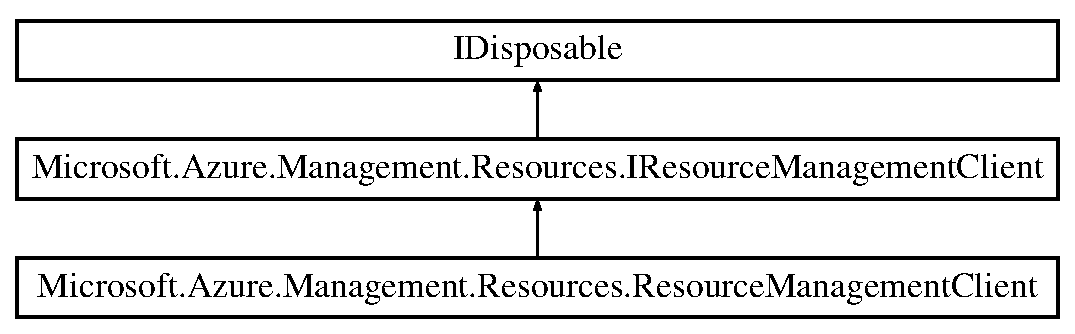
\includegraphics[height=3.000000cm]{interface_microsoft_1_1_azure_1_1_management_1_1_resources_1_1_i_resource_management_client}
\end{center}
\end{figure}
\subsection*{Properties}
\begin{DoxyCompactItemize}
\item 
Uri \hyperlink{interface_microsoft_1_1_azure_1_1_management_1_1_resources_1_1_i_resource_management_client_a699f3cec200fbb9f98993efa79126bf2}{Base\+Uri}\hspace{0.3cm}{\ttfamily  \mbox{[}get, set\mbox{]}}
\begin{DoxyCompactList}\small\item\em The base U\+RI of the service. \end{DoxyCompactList}\item 
Json\+Serializer\+Settings \hyperlink{interface_microsoft_1_1_azure_1_1_management_1_1_resources_1_1_i_resource_management_client_a7b8af6324e83c3bce910e351f6757de0}{Serialization\+Settings}\hspace{0.3cm}{\ttfamily  \mbox{[}get\mbox{]}}
\begin{DoxyCompactList}\small\item\em Gets or sets json serialization settings. \end{DoxyCompactList}\item 
Json\+Serializer\+Settings \hyperlink{interface_microsoft_1_1_azure_1_1_management_1_1_resources_1_1_i_resource_management_client_aaecdaf3a8d2fee75ceef11056cc9fff2}{Deserialization\+Settings}\hspace{0.3cm}{\ttfamily  \mbox{[}get\mbox{]}}
\begin{DoxyCompactList}\small\item\em Gets or sets json deserialization settings. \end{DoxyCompactList}\item 
Service\+Client\+Credentials \hyperlink{interface_microsoft_1_1_azure_1_1_management_1_1_resources_1_1_i_resource_management_client_a268fab051dd18cc4fd0ba8a38aaee3ea}{Credentials}\hspace{0.3cm}{\ttfamily  \mbox{[}get\mbox{]}}
\begin{DoxyCompactList}\small\item\em The management credentials for \hyperlink{namespace_microsoft_1_1_azure}{Azure}. \end{DoxyCompactList}\item 
string \hyperlink{interface_microsoft_1_1_azure_1_1_management_1_1_resources_1_1_i_resource_management_client_a4291b13a43108062ff778b2550972ed4}{Subscription\+Id}\hspace{0.3cm}{\ttfamily  \mbox{[}get, set\mbox{]}}
\begin{DoxyCompactList}\small\item\em Gets subscription credentials which uniquely identify \hyperlink{namespace_microsoft}{Microsoft} \hyperlink{namespace_microsoft_1_1_azure}{Azure} subscription. The subscription ID forms part of the U\+RI for every service call. \end{DoxyCompactList}\item 
string \hyperlink{interface_microsoft_1_1_azure_1_1_management_1_1_resources_1_1_i_resource_management_client_af0fe92fb0e05a0db48a8f81f9d9d0eda}{Api\+Version}\hspace{0.3cm}{\ttfamily  \mbox{[}get\mbox{]}}
\begin{DoxyCompactList}\small\item\em Client Api Version. \end{DoxyCompactList}\item 
string \hyperlink{interface_microsoft_1_1_azure_1_1_management_1_1_resources_1_1_i_resource_management_client_ad77527c37922f39b139a21d4c973d1fd}{Accept\+Language}\hspace{0.3cm}{\ttfamily  \mbox{[}get, set\mbox{]}}
\begin{DoxyCompactList}\small\item\em Gets or sets the preferred language for the response. \end{DoxyCompactList}\item 
int \hyperlink{interface_microsoft_1_1_azure_1_1_management_1_1_resources_1_1_i_resource_management_client_ad843dd318d88f4e31058ce9f0c7891a5}{Long\+Running\+Operation\+Retry\+Timeout}\hspace{0.3cm}{\ttfamily  \mbox{[}get, set\mbox{]}}
\begin{DoxyCompactList}\small\item\em The retry timeout for Long Running Operations. \end{DoxyCompactList}\item 
\hyperlink{interface_microsoft_1_1_azure_1_1_management_1_1_resources_1_1_i_deployments_operations}{I\+Deployments\+Operations} {\bfseries Deployments}\hspace{0.3cm}{\ttfamily  \mbox{[}get\mbox{]}}\hypertarget{interface_microsoft_1_1_azure_1_1_management_1_1_resources_1_1_i_resource_management_client_acf082411a76c642863ecae7ff22b4df5}{}\label{interface_microsoft_1_1_azure_1_1_management_1_1_resources_1_1_i_resource_management_client_acf082411a76c642863ecae7ff22b4df5}

\item 
\hyperlink{interface_microsoft_1_1_azure_1_1_management_1_1_resources_1_1_i_providers_operations}{I\+Providers\+Operations} {\bfseries Providers}\hspace{0.3cm}{\ttfamily  \mbox{[}get\mbox{]}}\hypertarget{interface_microsoft_1_1_azure_1_1_management_1_1_resources_1_1_i_resource_management_client_a6f04df75b1e982a749e101afa4758b8a}{}\label{interface_microsoft_1_1_azure_1_1_management_1_1_resources_1_1_i_resource_management_client_a6f04df75b1e982a749e101afa4758b8a}

\item 
\hyperlink{interface_microsoft_1_1_azure_1_1_management_1_1_resources_1_1_i_resource_groups_operations}{I\+Resource\+Groups\+Operations} {\bfseries Resource\+Groups}\hspace{0.3cm}{\ttfamily  \mbox{[}get\mbox{]}}\hypertarget{interface_microsoft_1_1_azure_1_1_management_1_1_resources_1_1_i_resource_management_client_a269196605e644ec85035b95eb9fccde4}{}\label{interface_microsoft_1_1_azure_1_1_management_1_1_resources_1_1_i_resource_management_client_a269196605e644ec85035b95eb9fccde4}

\item 
\hyperlink{interface_microsoft_1_1_azure_1_1_management_1_1_resources_1_1_i_resources_operations}{I\+Resources\+Operations} {\bfseries Resources}\hspace{0.3cm}{\ttfamily  \mbox{[}get\mbox{]}}\hypertarget{interface_microsoft_1_1_azure_1_1_management_1_1_resources_1_1_i_resource_management_client_a36ceba308a1fff084e2ddf5d10e33032}{}\label{interface_microsoft_1_1_azure_1_1_management_1_1_resources_1_1_i_resource_management_client_a36ceba308a1fff084e2ddf5d10e33032}

\item 
\hyperlink{interface_microsoft_1_1_azure_1_1_management_1_1_resources_1_1_i_tags_operations}{I\+Tags\+Operations} {\bfseries Tags}\hspace{0.3cm}{\ttfamily  \mbox{[}get\mbox{]}}\hypertarget{interface_microsoft_1_1_azure_1_1_management_1_1_resources_1_1_i_resource_management_client_afc5a408263bcf188b81069bc3da81fe1}{}\label{interface_microsoft_1_1_azure_1_1_management_1_1_resources_1_1_i_resource_management_client_afc5a408263bcf188b81069bc3da81fe1}

\item 
\hyperlink{interface_microsoft_1_1_azure_1_1_management_1_1_resources_1_1_i_deployment_operations_operations}{I\+Deployment\+Operations\+Operations} {\bfseries Deployment\+Operations}\hspace{0.3cm}{\ttfamily  \mbox{[}get\mbox{]}}\hypertarget{interface_microsoft_1_1_azure_1_1_management_1_1_resources_1_1_i_resource_management_client_a553e60bfee6e7c95677b0ea78246b736}{}\label{interface_microsoft_1_1_azure_1_1_management_1_1_resources_1_1_i_resource_management_client_a553e60bfee6e7c95677b0ea78246b736}

\item 
\hyperlink{interface_microsoft_1_1_azure_1_1_management_1_1_resources_1_1_i_resource_provider_operation_details_operations}{I\+Resource\+Provider\+Operation\+Details\+Operations} {\bfseries Resource\+Provider\+Operation\+Details}\hspace{0.3cm}{\ttfamily  \mbox{[}get\mbox{]}}\hypertarget{interface_microsoft_1_1_azure_1_1_management_1_1_resources_1_1_i_resource_management_client_a8301637dce94ad69927d725dc30db7d9}{}\label{interface_microsoft_1_1_azure_1_1_management_1_1_resources_1_1_i_resource_management_client_a8301637dce94ad69927d725dc30db7d9}

\item 
\hyperlink{interface_microsoft_1_1_azure_1_1_management_1_1_resources_1_1_i_policy_definitions_operations}{I\+Policy\+Definitions\+Operations} {\bfseries Policy\+Definitions}\hspace{0.3cm}{\ttfamily  \mbox{[}get\mbox{]}}\hypertarget{interface_microsoft_1_1_azure_1_1_management_1_1_resources_1_1_i_resource_management_client_abceaf6f434c1716d3ab8db01543d1fb3}{}\label{interface_microsoft_1_1_azure_1_1_management_1_1_resources_1_1_i_resource_management_client_abceaf6f434c1716d3ab8db01543d1fb3}

\item 
\hyperlink{interface_microsoft_1_1_azure_1_1_management_1_1_resources_1_1_i_policy_assignments_operations}{I\+Policy\+Assignments\+Operations} {\bfseries Policy\+Assignments}\hspace{0.3cm}{\ttfamily  \mbox{[}get\mbox{]}}\hypertarget{interface_microsoft_1_1_azure_1_1_management_1_1_resources_1_1_i_resource_management_client_a310626ebf6e4e98278d3b2f734f2ce95}{}\label{interface_microsoft_1_1_azure_1_1_management_1_1_resources_1_1_i_resource_management_client_a310626ebf6e4e98278d3b2f734f2ce95}

\end{DoxyCompactItemize}


\subsection{Detailed Description}




\subsection{Property Documentation}
\index{Microsoft\+::\+Azure\+::\+Management\+::\+Resources\+::\+I\+Resource\+Management\+Client@{Microsoft\+::\+Azure\+::\+Management\+::\+Resources\+::\+I\+Resource\+Management\+Client}!Accept\+Language@{Accept\+Language}}
\index{Accept\+Language@{Accept\+Language}!Microsoft\+::\+Azure\+::\+Management\+::\+Resources\+::\+I\+Resource\+Management\+Client@{Microsoft\+::\+Azure\+::\+Management\+::\+Resources\+::\+I\+Resource\+Management\+Client}}
\subsubsection[{\texorpdfstring{Accept\+Language}{AcceptLanguage}}]{\setlength{\rightskip}{0pt plus 5cm}string Microsoft.\+Azure.\+Management.\+Resources.\+I\+Resource\+Management\+Client.\+Accept\+Language\hspace{0.3cm}{\ttfamily [get]}, {\ttfamily [set]}}\hypertarget{interface_microsoft_1_1_azure_1_1_management_1_1_resources_1_1_i_resource_management_client_ad77527c37922f39b139a21d4c973d1fd}{}\label{interface_microsoft_1_1_azure_1_1_management_1_1_resources_1_1_i_resource_management_client_ad77527c37922f39b139a21d4c973d1fd}


Gets or sets the preferred language for the response. 

\index{Microsoft\+::\+Azure\+::\+Management\+::\+Resources\+::\+I\+Resource\+Management\+Client@{Microsoft\+::\+Azure\+::\+Management\+::\+Resources\+::\+I\+Resource\+Management\+Client}!Api\+Version@{Api\+Version}}
\index{Api\+Version@{Api\+Version}!Microsoft\+::\+Azure\+::\+Management\+::\+Resources\+::\+I\+Resource\+Management\+Client@{Microsoft\+::\+Azure\+::\+Management\+::\+Resources\+::\+I\+Resource\+Management\+Client}}
\subsubsection[{\texorpdfstring{Api\+Version}{ApiVersion}}]{\setlength{\rightskip}{0pt plus 5cm}string Microsoft.\+Azure.\+Management.\+Resources.\+I\+Resource\+Management\+Client.\+Api\+Version\hspace{0.3cm}{\ttfamily [get]}}\hypertarget{interface_microsoft_1_1_azure_1_1_management_1_1_resources_1_1_i_resource_management_client_af0fe92fb0e05a0db48a8f81f9d9d0eda}{}\label{interface_microsoft_1_1_azure_1_1_management_1_1_resources_1_1_i_resource_management_client_af0fe92fb0e05a0db48a8f81f9d9d0eda}


Client Api Version. 

\index{Microsoft\+::\+Azure\+::\+Management\+::\+Resources\+::\+I\+Resource\+Management\+Client@{Microsoft\+::\+Azure\+::\+Management\+::\+Resources\+::\+I\+Resource\+Management\+Client}!Base\+Uri@{Base\+Uri}}
\index{Base\+Uri@{Base\+Uri}!Microsoft\+::\+Azure\+::\+Management\+::\+Resources\+::\+I\+Resource\+Management\+Client@{Microsoft\+::\+Azure\+::\+Management\+::\+Resources\+::\+I\+Resource\+Management\+Client}}
\subsubsection[{\texorpdfstring{Base\+Uri}{BaseUri}}]{\setlength{\rightskip}{0pt plus 5cm}Uri Microsoft.\+Azure.\+Management.\+Resources.\+I\+Resource\+Management\+Client.\+Base\+Uri\hspace{0.3cm}{\ttfamily [get]}, {\ttfamily [set]}}\hypertarget{interface_microsoft_1_1_azure_1_1_management_1_1_resources_1_1_i_resource_management_client_a699f3cec200fbb9f98993efa79126bf2}{}\label{interface_microsoft_1_1_azure_1_1_management_1_1_resources_1_1_i_resource_management_client_a699f3cec200fbb9f98993efa79126bf2}


The base U\+RI of the service. 

\index{Microsoft\+::\+Azure\+::\+Management\+::\+Resources\+::\+I\+Resource\+Management\+Client@{Microsoft\+::\+Azure\+::\+Management\+::\+Resources\+::\+I\+Resource\+Management\+Client}!Credentials@{Credentials}}
\index{Credentials@{Credentials}!Microsoft\+::\+Azure\+::\+Management\+::\+Resources\+::\+I\+Resource\+Management\+Client@{Microsoft\+::\+Azure\+::\+Management\+::\+Resources\+::\+I\+Resource\+Management\+Client}}
\subsubsection[{\texorpdfstring{Credentials}{Credentials}}]{\setlength{\rightskip}{0pt plus 5cm}Service\+Client\+Credentials Microsoft.\+Azure.\+Management.\+Resources.\+I\+Resource\+Management\+Client.\+Credentials\hspace{0.3cm}{\ttfamily [get]}}\hypertarget{interface_microsoft_1_1_azure_1_1_management_1_1_resources_1_1_i_resource_management_client_a268fab051dd18cc4fd0ba8a38aaee3ea}{}\label{interface_microsoft_1_1_azure_1_1_management_1_1_resources_1_1_i_resource_management_client_a268fab051dd18cc4fd0ba8a38aaee3ea}


The management credentials for \hyperlink{namespace_microsoft_1_1_azure}{Azure}. 

\index{Microsoft\+::\+Azure\+::\+Management\+::\+Resources\+::\+I\+Resource\+Management\+Client@{Microsoft\+::\+Azure\+::\+Management\+::\+Resources\+::\+I\+Resource\+Management\+Client}!Deserialization\+Settings@{Deserialization\+Settings}}
\index{Deserialization\+Settings@{Deserialization\+Settings}!Microsoft\+::\+Azure\+::\+Management\+::\+Resources\+::\+I\+Resource\+Management\+Client@{Microsoft\+::\+Azure\+::\+Management\+::\+Resources\+::\+I\+Resource\+Management\+Client}}
\subsubsection[{\texorpdfstring{Deserialization\+Settings}{DeserializationSettings}}]{\setlength{\rightskip}{0pt plus 5cm}Json\+Serializer\+Settings Microsoft.\+Azure.\+Management.\+Resources.\+I\+Resource\+Management\+Client.\+Deserialization\+Settings\hspace{0.3cm}{\ttfamily [get]}}\hypertarget{interface_microsoft_1_1_azure_1_1_management_1_1_resources_1_1_i_resource_management_client_aaecdaf3a8d2fee75ceef11056cc9fff2}{}\label{interface_microsoft_1_1_azure_1_1_management_1_1_resources_1_1_i_resource_management_client_aaecdaf3a8d2fee75ceef11056cc9fff2}


Gets or sets json deserialization settings. 

\index{Microsoft\+::\+Azure\+::\+Management\+::\+Resources\+::\+I\+Resource\+Management\+Client@{Microsoft\+::\+Azure\+::\+Management\+::\+Resources\+::\+I\+Resource\+Management\+Client}!Long\+Running\+Operation\+Retry\+Timeout@{Long\+Running\+Operation\+Retry\+Timeout}}
\index{Long\+Running\+Operation\+Retry\+Timeout@{Long\+Running\+Operation\+Retry\+Timeout}!Microsoft\+::\+Azure\+::\+Management\+::\+Resources\+::\+I\+Resource\+Management\+Client@{Microsoft\+::\+Azure\+::\+Management\+::\+Resources\+::\+I\+Resource\+Management\+Client}}
\subsubsection[{\texorpdfstring{Long\+Running\+Operation\+Retry\+Timeout}{LongRunningOperationRetryTimeout}}]{\setlength{\rightskip}{0pt plus 5cm}int Microsoft.\+Azure.\+Management.\+Resources.\+I\+Resource\+Management\+Client.\+Long\+Running\+Operation\+Retry\+Timeout\hspace{0.3cm}{\ttfamily [get]}, {\ttfamily [set]}}\hypertarget{interface_microsoft_1_1_azure_1_1_management_1_1_resources_1_1_i_resource_management_client_ad843dd318d88f4e31058ce9f0c7891a5}{}\label{interface_microsoft_1_1_azure_1_1_management_1_1_resources_1_1_i_resource_management_client_ad843dd318d88f4e31058ce9f0c7891a5}


The retry timeout for Long Running Operations. 

\index{Microsoft\+::\+Azure\+::\+Management\+::\+Resources\+::\+I\+Resource\+Management\+Client@{Microsoft\+::\+Azure\+::\+Management\+::\+Resources\+::\+I\+Resource\+Management\+Client}!Serialization\+Settings@{Serialization\+Settings}}
\index{Serialization\+Settings@{Serialization\+Settings}!Microsoft\+::\+Azure\+::\+Management\+::\+Resources\+::\+I\+Resource\+Management\+Client@{Microsoft\+::\+Azure\+::\+Management\+::\+Resources\+::\+I\+Resource\+Management\+Client}}
\subsubsection[{\texorpdfstring{Serialization\+Settings}{SerializationSettings}}]{\setlength{\rightskip}{0pt plus 5cm}Json\+Serializer\+Settings Microsoft.\+Azure.\+Management.\+Resources.\+I\+Resource\+Management\+Client.\+Serialization\+Settings\hspace{0.3cm}{\ttfamily [get]}}\hypertarget{interface_microsoft_1_1_azure_1_1_management_1_1_resources_1_1_i_resource_management_client_a7b8af6324e83c3bce910e351f6757de0}{}\label{interface_microsoft_1_1_azure_1_1_management_1_1_resources_1_1_i_resource_management_client_a7b8af6324e83c3bce910e351f6757de0}


Gets or sets json serialization settings. 

\index{Microsoft\+::\+Azure\+::\+Management\+::\+Resources\+::\+I\+Resource\+Management\+Client@{Microsoft\+::\+Azure\+::\+Management\+::\+Resources\+::\+I\+Resource\+Management\+Client}!Subscription\+Id@{Subscription\+Id}}
\index{Subscription\+Id@{Subscription\+Id}!Microsoft\+::\+Azure\+::\+Management\+::\+Resources\+::\+I\+Resource\+Management\+Client@{Microsoft\+::\+Azure\+::\+Management\+::\+Resources\+::\+I\+Resource\+Management\+Client}}
\subsubsection[{\texorpdfstring{Subscription\+Id}{SubscriptionId}}]{\setlength{\rightskip}{0pt plus 5cm}string Microsoft.\+Azure.\+Management.\+Resources.\+I\+Resource\+Management\+Client.\+Subscription\+Id\hspace{0.3cm}{\ttfamily [get]}, {\ttfamily [set]}}\hypertarget{interface_microsoft_1_1_azure_1_1_management_1_1_resources_1_1_i_resource_management_client_a4291b13a43108062ff778b2550972ed4}{}\label{interface_microsoft_1_1_azure_1_1_management_1_1_resources_1_1_i_resource_management_client_a4291b13a43108062ff778b2550972ed4}


Gets subscription credentials which uniquely identify \hyperlink{namespace_microsoft}{Microsoft} \hyperlink{namespace_microsoft_1_1_azure}{Azure} subscription. The subscription ID forms part of the U\+RI for every service call. 



The documentation for this interface was generated from the following file\+:\begin{DoxyCompactItemize}
\item 
files/I\+Resource\+Management\+Client.\+cs\end{DoxyCompactItemize}

\hypertarget{interface_microsoft_1_1_azure_1_1_management_1_1_resources_1_1_i_resource_provider_operation_details_operations}{}\section{Microsoft.\+Azure.\+Management.\+Resources.\+I\+Resource\+Provider\+Operation\+Details\+Operations Interface Reference}
\label{interface_microsoft_1_1_azure_1_1_management_1_1_resources_1_1_i_resource_provider_operation_details_operations}\index{Microsoft.\+Azure.\+Management.\+Resources.\+I\+Resource\+Provider\+Operation\+Details\+Operations@{Microsoft.\+Azure.\+Management.\+Resources.\+I\+Resource\+Provider\+Operation\+Details\+Operations}}


Resource\+Provider\+Operation\+Details\+Operations operations.  




Inherited by Microsoft.\+Azure.\+Management.\+Resources.\+Resource\+Provider\+Operation\+Details\+Operations.

\subsection*{Public Member Functions}
\begin{DoxyCompactItemize}
\item 
Task$<$ Azure\+Operation\+Response$<$ I\+Page$<$ Resource\+Provider\+Operation\+Definition $>$ $>$ $>$ \hyperlink{interface_microsoft_1_1_azure_1_1_management_1_1_resources_1_1_i_resource_provider_operation_details_operations_aa96a381f62b0aa608a84a6b347167ee9}{List\+With\+Http\+Messages\+Async} (string resource\+Provider\+Namespace, string api\+Version, Dictionary$<$ string, List$<$ string $>$$>$ custom\+Headers=null, Cancellation\+Token cancellation\+Token=default(Cancellation\+Token))
\begin{DoxyCompactList}\small\item\em Gets a list of resource providers. \end{DoxyCompactList}\item 
Task$<$ Azure\+Operation\+Response$<$ I\+Page$<$ Resource\+Provider\+Operation\+Definition $>$ $>$ $>$ \hyperlink{interface_microsoft_1_1_azure_1_1_management_1_1_resources_1_1_i_resource_provider_operation_details_operations_aad57181801ce966de4020eea5cd96d27}{List\+Next\+With\+Http\+Messages\+Async} (string next\+Page\+Link, Dictionary$<$ string, List$<$ string $>$$>$ custom\+Headers=null, Cancellation\+Token cancellation\+Token=default(Cancellation\+Token))
\begin{DoxyCompactList}\small\item\em Gets a list of resource providers. \end{DoxyCompactList}\end{DoxyCompactItemize}


\subsection{Detailed Description}
Resource\+Provider\+Operation\+Details\+Operations operations. 



\subsection{Member Function Documentation}
\index{Microsoft\+::\+Azure\+::\+Management\+::\+Resources\+::\+I\+Resource\+Provider\+Operation\+Details\+Operations@{Microsoft\+::\+Azure\+::\+Management\+::\+Resources\+::\+I\+Resource\+Provider\+Operation\+Details\+Operations}!List\+Next\+With\+Http\+Messages\+Async@{List\+Next\+With\+Http\+Messages\+Async}}
\index{List\+Next\+With\+Http\+Messages\+Async@{List\+Next\+With\+Http\+Messages\+Async}!Microsoft\+::\+Azure\+::\+Management\+::\+Resources\+::\+I\+Resource\+Provider\+Operation\+Details\+Operations@{Microsoft\+::\+Azure\+::\+Management\+::\+Resources\+::\+I\+Resource\+Provider\+Operation\+Details\+Operations}}
\subsubsection[{\texorpdfstring{List\+Next\+With\+Http\+Messages\+Async(string next\+Page\+Link, Dictionary$<$ string, List$<$ string $>$$>$ custom\+Headers=null, Cancellation\+Token cancellation\+Token=default(\+Cancellation\+Token))}{ListNextWithHttpMessagesAsync(string nextPageLink, Dictionary< string, List< string >> customHeaders=null, CancellationToken cancellationToken=default(CancellationToken))}}]{\setlength{\rightskip}{0pt plus 5cm}Task$<$Azure\+Operation\+Response$<$I\+Page$<$Resource\+Provider\+Operation\+Definition$>$ $>$ $>$ Microsoft.\+Azure.\+Management.\+Resources.\+I\+Resource\+Provider\+Operation\+Details\+Operations.\+List\+Next\+With\+Http\+Messages\+Async (
\begin{DoxyParamCaption}
\item[{string}]{next\+Page\+Link, }
\item[{Dictionary$<$ string, List$<$ string $>$$>$}]{custom\+Headers = {\ttfamily null}, }
\item[{Cancellation\+Token}]{cancellation\+Token = {\ttfamily default(CancellationToken)}}
\end{DoxyParamCaption}
)}\hypertarget{interface_microsoft_1_1_azure_1_1_management_1_1_resources_1_1_i_resource_provider_operation_details_operations_aad57181801ce966de4020eea5cd96d27}{}\label{interface_microsoft_1_1_azure_1_1_management_1_1_resources_1_1_i_resource_provider_operation_details_operations_aad57181801ce966de4020eea5cd96d27}


Gets a list of resource providers. 


\begin{DoxyParams}{Parameters}
{\em next\+Page\+Link} & The Next\+Link from the previous successful call to List operation. \\
\hline
{\em custom\+Headers} & The headers that will be added to request. \\
\hline
{\em cancellation\+Token} & The cancellation token. \\
\hline
\end{DoxyParams}
\index{Microsoft\+::\+Azure\+::\+Management\+::\+Resources\+::\+I\+Resource\+Provider\+Operation\+Details\+Operations@{Microsoft\+::\+Azure\+::\+Management\+::\+Resources\+::\+I\+Resource\+Provider\+Operation\+Details\+Operations}!List\+With\+Http\+Messages\+Async@{List\+With\+Http\+Messages\+Async}}
\index{List\+With\+Http\+Messages\+Async@{List\+With\+Http\+Messages\+Async}!Microsoft\+::\+Azure\+::\+Management\+::\+Resources\+::\+I\+Resource\+Provider\+Operation\+Details\+Operations@{Microsoft\+::\+Azure\+::\+Management\+::\+Resources\+::\+I\+Resource\+Provider\+Operation\+Details\+Operations}}
\subsubsection[{\texorpdfstring{List\+With\+Http\+Messages\+Async(string resource\+Provider\+Namespace, string api\+Version, Dictionary$<$ string, List$<$ string $>$$>$ custom\+Headers=null, Cancellation\+Token cancellation\+Token=default(\+Cancellation\+Token))}{ListWithHttpMessagesAsync(string resourceProviderNamespace, string apiVersion, Dictionary< string, List< string >> customHeaders=null, CancellationToken cancellationToken=default(CancellationToken))}}]{\setlength{\rightskip}{0pt plus 5cm}Task$<$Azure\+Operation\+Response$<$I\+Page$<$Resource\+Provider\+Operation\+Definition$>$ $>$ $>$ Microsoft.\+Azure.\+Management.\+Resources.\+I\+Resource\+Provider\+Operation\+Details\+Operations.\+List\+With\+Http\+Messages\+Async (
\begin{DoxyParamCaption}
\item[{string}]{resource\+Provider\+Namespace, }
\item[{string}]{api\+Version, }
\item[{Dictionary$<$ string, List$<$ string $>$$>$}]{custom\+Headers = {\ttfamily null}, }
\item[{Cancellation\+Token}]{cancellation\+Token = {\ttfamily default(CancellationToken)}}
\end{DoxyParamCaption}
)}\hypertarget{interface_microsoft_1_1_azure_1_1_management_1_1_resources_1_1_i_resource_provider_operation_details_operations_aa96a381f62b0aa608a84a6b347167ee9}{}\label{interface_microsoft_1_1_azure_1_1_management_1_1_resources_1_1_i_resource_provider_operation_details_operations_aa96a381f62b0aa608a84a6b347167ee9}


Gets a list of resource providers. 


\begin{DoxyParams}{Parameters}
{\em resource\+Provider\+Namespace} & Resource identity. \\
\hline
{\em api\+Version} & \\
\hline
{\em custom\+Headers} & The headers that will be added to request. \\
\hline
{\em cancellation\+Token} & The cancellation token. \\
\hline
\end{DoxyParams}


The documentation for this interface was generated from the following file\+:\begin{DoxyCompactItemize}
\item 
files/I\+Resource\+Provider\+Operation\+Details\+Operations.\+cs\end{DoxyCompactItemize}

\hypertarget{interface_microsoft_1_1_azure_1_1_management_1_1_resources_1_1_i_resources_operations}{}\section{Microsoft.\+Azure.\+Management.\+Resources.\+I\+Resources\+Operations Interface Reference}
\label{interface_microsoft_1_1_azure_1_1_management_1_1_resources_1_1_i_resources_operations}\index{Microsoft.\+Azure.\+Management.\+Resources.\+I\+Resources\+Operations@{Microsoft.\+Azure.\+Management.\+Resources.\+I\+Resources\+Operations}}


Resources\+Operations operations.  




Inherited by Microsoft.\+Azure.\+Management.\+Resources.\+Resources\+Operations.

\subsection*{Public Member Functions}
\begin{DoxyCompactItemize}
\item 
Task$<$ Azure\+Operation\+Response $>$ \hyperlink{interface_microsoft_1_1_azure_1_1_management_1_1_resources_1_1_i_resources_operations_ab3647d8555b725c25a5bdb5c20eb2c99}{Move\+Resources\+With\+Http\+Messages\+Async} (string source\+Resource\+Group\+Name, Resources\+Move\+Info parameters, Dictionary$<$ string, List$<$ string $>$$>$ custom\+Headers=null, Cancellation\+Token cancellation\+Token=default(Cancellation\+Token))
\begin{DoxyCompactList}\small\item\em Begin moving resources.\+To determine whether the operation has finished processing the request, call Get\+Long\+Running\+Operation\+Status. \end{DoxyCompactList}\item 
Task$<$ Azure\+Operation\+Response $>$ \hyperlink{interface_microsoft_1_1_azure_1_1_management_1_1_resources_1_1_i_resources_operations_a91f9b53e79a6400d10ef279b05626142}{Begin\+Move\+Resources\+With\+Http\+Messages\+Async} (string source\+Resource\+Group\+Name, Resources\+Move\+Info parameters, Dictionary$<$ string, List$<$ string $>$$>$ custom\+Headers=null, Cancellation\+Token cancellation\+Token=default(Cancellation\+Token))
\begin{DoxyCompactList}\small\item\em Begin moving resources.\+To determine whether the operation has finished processing the request, call Get\+Long\+Running\+Operation\+Status. \end{DoxyCompactList}\item 
Task$<$ Azure\+Operation\+Response$<$ I\+Page$<$ Generic\+Resource $>$ $>$ $>$ \hyperlink{interface_microsoft_1_1_azure_1_1_management_1_1_resources_1_1_i_resources_operations_a579be7fe62d7be2d7d8515937b4e79f9}{List\+With\+Http\+Messages\+Async} (O\+Data\+Query$<$ Generic\+Resource\+Filter $>$ odata\+Query=default(O\+Data\+Query$<$ Generic\+Resource\+Filter $>$), Dictionary$<$ string, List$<$ string $>$$>$ custom\+Headers=null, Cancellation\+Token cancellation\+Token=default(Cancellation\+Token))
\begin{DoxyCompactList}\small\item\em Get all of the resources under a subscription. \end{DoxyCompactList}\item 
Task$<$ Azure\+Operation\+Response$<$ bool?$>$ $>$ \hyperlink{interface_microsoft_1_1_azure_1_1_management_1_1_resources_1_1_i_resources_operations_a50737970171c867340354e6e8c054a25}{Check\+Existence\+With\+Http\+Messages\+Async} (string resource\+Group\+Name, string resource\+Provider\+Namespace, string parent\+Resource\+Path, string resource\+Type, string resource\+Name, string api\+Version, Dictionary$<$ string, List$<$ string $>$$>$ custom\+Headers=null, Cancellation\+Token cancellation\+Token=default(Cancellation\+Token))
\begin{DoxyCompactList}\small\item\em Checks whether resource exists. \end{DoxyCompactList}\item 
Task$<$ Azure\+Operation\+Response $>$ \hyperlink{interface_microsoft_1_1_azure_1_1_management_1_1_resources_1_1_i_resources_operations_a5f298dc644e07c3e58cb0c89618af813}{Delete\+With\+Http\+Messages\+Async} (string resource\+Group\+Name, string resource\+Provider\+Namespace, string parent\+Resource\+Path, string resource\+Type, string resource\+Name, string api\+Version, Dictionary$<$ string, List$<$ string $>$$>$ custom\+Headers=null, Cancellation\+Token cancellation\+Token=default(Cancellation\+Token))
\begin{DoxyCompactList}\small\item\em Delete resource and all of its resources. \end{DoxyCompactList}\item 
Task$<$ Azure\+Operation\+Response$<$ Generic\+Resource $>$ $>$ \hyperlink{interface_microsoft_1_1_azure_1_1_management_1_1_resources_1_1_i_resources_operations_ae3d904d272734f1d9706a778a8f113ac}{Create\+Or\+Update\+With\+Http\+Messages\+Async} (string resource\+Group\+Name, string resource\+Provider\+Namespace, string parent\+Resource\+Path, string resource\+Type, string resource\+Name, string api\+Version, Generic\+Resource parameters, Dictionary$<$ string, List$<$ string $>$$>$ custom\+Headers=null, Cancellation\+Token cancellation\+Token=default(Cancellation\+Token))
\begin{DoxyCompactList}\small\item\em Create a resource. \end{DoxyCompactList}\item 
Task$<$ Azure\+Operation\+Response$<$ Generic\+Resource $>$ $>$ \hyperlink{interface_microsoft_1_1_azure_1_1_management_1_1_resources_1_1_i_resources_operations_a9c1dc263922de3e9a71c22e7e1a95a91}{Get\+With\+Http\+Messages\+Async} (string resource\+Group\+Name, string resource\+Provider\+Namespace, string parent\+Resource\+Path, string resource\+Type, string resource\+Name, string api\+Version, Dictionary$<$ string, List$<$ string $>$$>$ custom\+Headers=null, Cancellation\+Token cancellation\+Token=default(Cancellation\+Token))
\begin{DoxyCompactList}\small\item\em Returns a resource belonging to a resource group. \end{DoxyCompactList}\item 
Task$<$ Azure\+Operation\+Response$<$ I\+Page$<$ Generic\+Resource $>$ $>$ $>$ \hyperlink{interface_microsoft_1_1_azure_1_1_management_1_1_resources_1_1_i_resources_operations_abb4049749687f1b577514aff8af104fc}{List\+Next\+With\+Http\+Messages\+Async} (string next\+Page\+Link, Dictionary$<$ string, List$<$ string $>$$>$ custom\+Headers=null, Cancellation\+Token cancellation\+Token=default(Cancellation\+Token))
\begin{DoxyCompactList}\small\item\em Get all of the resources under a subscription. \end{DoxyCompactList}\end{DoxyCompactItemize}


\subsection{Detailed Description}
Resources\+Operations operations. 



\subsection{Member Function Documentation}
\index{Microsoft\+::\+Azure\+::\+Management\+::\+Resources\+::\+I\+Resources\+Operations@{Microsoft\+::\+Azure\+::\+Management\+::\+Resources\+::\+I\+Resources\+Operations}!Begin\+Move\+Resources\+With\+Http\+Messages\+Async@{Begin\+Move\+Resources\+With\+Http\+Messages\+Async}}
\index{Begin\+Move\+Resources\+With\+Http\+Messages\+Async@{Begin\+Move\+Resources\+With\+Http\+Messages\+Async}!Microsoft\+::\+Azure\+::\+Management\+::\+Resources\+::\+I\+Resources\+Operations@{Microsoft\+::\+Azure\+::\+Management\+::\+Resources\+::\+I\+Resources\+Operations}}
\subsubsection[{\texorpdfstring{Begin\+Move\+Resources\+With\+Http\+Messages\+Async(string source\+Resource\+Group\+Name, Resources\+Move\+Info parameters, Dictionary$<$ string, List$<$ string $>$$>$ custom\+Headers=null, Cancellation\+Token cancellation\+Token=default(\+Cancellation\+Token))}{BeginMoveResourcesWithHttpMessagesAsync(string sourceResourceGroupName, ResourcesMoveInfo parameters, Dictionary< string, List< string >> customHeaders=null, CancellationToken cancellationToken=default(CancellationToken))}}]{\setlength{\rightskip}{0pt plus 5cm}Task$<$Azure\+Operation\+Response$>$ Microsoft.\+Azure.\+Management.\+Resources.\+I\+Resources\+Operations.\+Begin\+Move\+Resources\+With\+Http\+Messages\+Async (
\begin{DoxyParamCaption}
\item[{string}]{source\+Resource\+Group\+Name, }
\item[{Resources\+Move\+Info}]{parameters, }
\item[{Dictionary$<$ string, List$<$ string $>$$>$}]{custom\+Headers = {\ttfamily null}, }
\item[{Cancellation\+Token}]{cancellation\+Token = {\ttfamily default(CancellationToken)}}
\end{DoxyParamCaption}
)}\hypertarget{interface_microsoft_1_1_azure_1_1_management_1_1_resources_1_1_i_resources_operations_a91f9b53e79a6400d10ef279b05626142}{}\label{interface_microsoft_1_1_azure_1_1_management_1_1_resources_1_1_i_resources_operations_a91f9b53e79a6400d10ef279b05626142}


Begin moving resources.\+To determine whether the operation has finished processing the request, call Get\+Long\+Running\+Operation\+Status. 


\begin{DoxyParams}{Parameters}
{\em source\+Resource\+Group\+Name} & Source resource group name. \\
\hline
{\em parameters} & move resources\textquotesingle{} parameters. \\
\hline
{\em custom\+Headers} & The headers that will be added to request. \\
\hline
{\em cancellation\+Token} & The cancellation token. \\
\hline
\end{DoxyParams}
\index{Microsoft\+::\+Azure\+::\+Management\+::\+Resources\+::\+I\+Resources\+Operations@{Microsoft\+::\+Azure\+::\+Management\+::\+Resources\+::\+I\+Resources\+Operations}!Check\+Existence\+With\+Http\+Messages\+Async@{Check\+Existence\+With\+Http\+Messages\+Async}}
\index{Check\+Existence\+With\+Http\+Messages\+Async@{Check\+Existence\+With\+Http\+Messages\+Async}!Microsoft\+::\+Azure\+::\+Management\+::\+Resources\+::\+I\+Resources\+Operations@{Microsoft\+::\+Azure\+::\+Management\+::\+Resources\+::\+I\+Resources\+Operations}}
\subsubsection[{\texorpdfstring{Check\+Existence\+With\+Http\+Messages\+Async(string resource\+Group\+Name, string resource\+Provider\+Namespace, string parent\+Resource\+Path, string resource\+Type, string resource\+Name, string api\+Version, Dictionary$<$ string, List$<$ string $>$$>$ custom\+Headers=null, Cancellation\+Token cancellation\+Token=default(\+Cancellation\+Token))}{CheckExistenceWithHttpMessagesAsync(string resourceGroupName, string resourceProviderNamespace, string parentResourcePath, string resourceType, string resourceName, string apiVersion, Dictionary< string, List< string >> customHeaders=null, CancellationToken cancellationToken=default(CancellationToken))}}]{\setlength{\rightskip}{0pt plus 5cm}Task$<$Azure\+Operation\+Response$<$bool?$>$ $>$ Microsoft.\+Azure.\+Management.\+Resources.\+I\+Resources\+Operations.\+Check\+Existence\+With\+Http\+Messages\+Async (
\begin{DoxyParamCaption}
\item[{string}]{resource\+Group\+Name, }
\item[{string}]{resource\+Provider\+Namespace, }
\item[{string}]{parent\+Resource\+Path, }
\item[{string}]{resource\+Type, }
\item[{string}]{resource\+Name, }
\item[{string}]{api\+Version, }
\item[{Dictionary$<$ string, List$<$ string $>$$>$}]{custom\+Headers = {\ttfamily null}, }
\item[{Cancellation\+Token}]{cancellation\+Token = {\ttfamily default(CancellationToken)}}
\end{DoxyParamCaption}
)}\hypertarget{interface_microsoft_1_1_azure_1_1_management_1_1_resources_1_1_i_resources_operations_a50737970171c867340354e6e8c054a25}{}\label{interface_microsoft_1_1_azure_1_1_management_1_1_resources_1_1_i_resources_operations_a50737970171c867340354e6e8c054a25}


Checks whether resource exists. 


\begin{DoxyParams}{Parameters}
{\em resource\+Group\+Name} & The name of the resource group. The name is case insensitive. \\
\hline
{\em resource\+Provider\+Namespace} & Resource identity. \\
\hline
{\em parent\+Resource\+Path} & Resource identity. \\
\hline
{\em resource\+Type} & Resource identity. \\
\hline
{\em resource\+Name} & Resource identity. \\
\hline
{\em api\+Version} & \\
\hline
{\em custom\+Headers} & The headers that will be added to request. \\
\hline
{\em cancellation\+Token} & The cancellation token. \\
\hline
\end{DoxyParams}
\index{Microsoft\+::\+Azure\+::\+Management\+::\+Resources\+::\+I\+Resources\+Operations@{Microsoft\+::\+Azure\+::\+Management\+::\+Resources\+::\+I\+Resources\+Operations}!Create\+Or\+Update\+With\+Http\+Messages\+Async@{Create\+Or\+Update\+With\+Http\+Messages\+Async}}
\index{Create\+Or\+Update\+With\+Http\+Messages\+Async@{Create\+Or\+Update\+With\+Http\+Messages\+Async}!Microsoft\+::\+Azure\+::\+Management\+::\+Resources\+::\+I\+Resources\+Operations@{Microsoft\+::\+Azure\+::\+Management\+::\+Resources\+::\+I\+Resources\+Operations}}
\subsubsection[{\texorpdfstring{Create\+Or\+Update\+With\+Http\+Messages\+Async(string resource\+Group\+Name, string resource\+Provider\+Namespace, string parent\+Resource\+Path, string resource\+Type, string resource\+Name, string api\+Version, Generic\+Resource parameters, Dictionary$<$ string, List$<$ string $>$$>$ custom\+Headers=null, Cancellation\+Token cancellation\+Token=default(\+Cancellation\+Token))}{CreateOrUpdateWithHttpMessagesAsync(string resourceGroupName, string resourceProviderNamespace, string parentResourcePath, string resourceType, string resourceName, string apiVersion, GenericResource parameters, Dictionary< string, List< string >> customHeaders=null, CancellationToken cancellationToken=default(CancellationToken))}}]{\setlength{\rightskip}{0pt plus 5cm}Task$<$Azure\+Operation\+Response$<$Generic\+Resource$>$ $>$ Microsoft.\+Azure.\+Management.\+Resources.\+I\+Resources\+Operations.\+Create\+Or\+Update\+With\+Http\+Messages\+Async (
\begin{DoxyParamCaption}
\item[{string}]{resource\+Group\+Name, }
\item[{string}]{resource\+Provider\+Namespace, }
\item[{string}]{parent\+Resource\+Path, }
\item[{string}]{resource\+Type, }
\item[{string}]{resource\+Name, }
\item[{string}]{api\+Version, }
\item[{Generic\+Resource}]{parameters, }
\item[{Dictionary$<$ string, List$<$ string $>$$>$}]{custom\+Headers = {\ttfamily null}, }
\item[{Cancellation\+Token}]{cancellation\+Token = {\ttfamily default(CancellationToken)}}
\end{DoxyParamCaption}
)}\hypertarget{interface_microsoft_1_1_azure_1_1_management_1_1_resources_1_1_i_resources_operations_ae3d904d272734f1d9706a778a8f113ac}{}\label{interface_microsoft_1_1_azure_1_1_management_1_1_resources_1_1_i_resources_operations_ae3d904d272734f1d9706a778a8f113ac}


Create a resource. 


\begin{DoxyParams}{Parameters}
{\em resource\+Group\+Name} & The name of the resource group. The name is case insensitive. \\
\hline
{\em resource\+Provider\+Namespace} & Resource identity. \\
\hline
{\em parent\+Resource\+Path} & Resource identity. \\
\hline
{\em resource\+Type} & Resource identity. \\
\hline
{\em resource\+Name} & Resource identity. \\
\hline
{\em api\+Version} & \\
\hline
{\em parameters} & Create or update resource parameters. \\
\hline
{\em custom\+Headers} & The headers that will be added to request. \\
\hline
{\em cancellation\+Token} & The cancellation token. \\
\hline
\end{DoxyParams}
\index{Microsoft\+::\+Azure\+::\+Management\+::\+Resources\+::\+I\+Resources\+Operations@{Microsoft\+::\+Azure\+::\+Management\+::\+Resources\+::\+I\+Resources\+Operations}!Delete\+With\+Http\+Messages\+Async@{Delete\+With\+Http\+Messages\+Async}}
\index{Delete\+With\+Http\+Messages\+Async@{Delete\+With\+Http\+Messages\+Async}!Microsoft\+::\+Azure\+::\+Management\+::\+Resources\+::\+I\+Resources\+Operations@{Microsoft\+::\+Azure\+::\+Management\+::\+Resources\+::\+I\+Resources\+Operations}}
\subsubsection[{\texorpdfstring{Delete\+With\+Http\+Messages\+Async(string resource\+Group\+Name, string resource\+Provider\+Namespace, string parent\+Resource\+Path, string resource\+Type, string resource\+Name, string api\+Version, Dictionary$<$ string, List$<$ string $>$$>$ custom\+Headers=null, Cancellation\+Token cancellation\+Token=default(\+Cancellation\+Token))}{DeleteWithHttpMessagesAsync(string resourceGroupName, string resourceProviderNamespace, string parentResourcePath, string resourceType, string resourceName, string apiVersion, Dictionary< string, List< string >> customHeaders=null, CancellationToken cancellationToken=default(CancellationToken))}}]{\setlength{\rightskip}{0pt plus 5cm}Task$<$Azure\+Operation\+Response$>$ Microsoft.\+Azure.\+Management.\+Resources.\+I\+Resources\+Operations.\+Delete\+With\+Http\+Messages\+Async (
\begin{DoxyParamCaption}
\item[{string}]{resource\+Group\+Name, }
\item[{string}]{resource\+Provider\+Namespace, }
\item[{string}]{parent\+Resource\+Path, }
\item[{string}]{resource\+Type, }
\item[{string}]{resource\+Name, }
\item[{string}]{api\+Version, }
\item[{Dictionary$<$ string, List$<$ string $>$$>$}]{custom\+Headers = {\ttfamily null}, }
\item[{Cancellation\+Token}]{cancellation\+Token = {\ttfamily default(CancellationToken)}}
\end{DoxyParamCaption}
)}\hypertarget{interface_microsoft_1_1_azure_1_1_management_1_1_resources_1_1_i_resources_operations_a5f298dc644e07c3e58cb0c89618af813}{}\label{interface_microsoft_1_1_azure_1_1_management_1_1_resources_1_1_i_resources_operations_a5f298dc644e07c3e58cb0c89618af813}


Delete resource and all of its resources. 


\begin{DoxyParams}{Parameters}
{\em resource\+Group\+Name} & The name of the resource group. The name is case insensitive. \\
\hline
{\em resource\+Provider\+Namespace} & Resource identity. \\
\hline
{\em parent\+Resource\+Path} & Resource identity. \\
\hline
{\em resource\+Type} & Resource identity. \\
\hline
{\em resource\+Name} & Resource identity. \\
\hline
{\em api\+Version} & \\
\hline
{\em custom\+Headers} & The headers that will be added to request. \\
\hline
{\em cancellation\+Token} & The cancellation token. \\
\hline
\end{DoxyParams}
\index{Microsoft\+::\+Azure\+::\+Management\+::\+Resources\+::\+I\+Resources\+Operations@{Microsoft\+::\+Azure\+::\+Management\+::\+Resources\+::\+I\+Resources\+Operations}!Get\+With\+Http\+Messages\+Async@{Get\+With\+Http\+Messages\+Async}}
\index{Get\+With\+Http\+Messages\+Async@{Get\+With\+Http\+Messages\+Async}!Microsoft\+::\+Azure\+::\+Management\+::\+Resources\+::\+I\+Resources\+Operations@{Microsoft\+::\+Azure\+::\+Management\+::\+Resources\+::\+I\+Resources\+Operations}}
\subsubsection[{\texorpdfstring{Get\+With\+Http\+Messages\+Async(string resource\+Group\+Name, string resource\+Provider\+Namespace, string parent\+Resource\+Path, string resource\+Type, string resource\+Name, string api\+Version, Dictionary$<$ string, List$<$ string $>$$>$ custom\+Headers=null, Cancellation\+Token cancellation\+Token=default(\+Cancellation\+Token))}{GetWithHttpMessagesAsync(string resourceGroupName, string resourceProviderNamespace, string parentResourcePath, string resourceType, string resourceName, string apiVersion, Dictionary< string, List< string >> customHeaders=null, CancellationToken cancellationToken=default(CancellationToken))}}]{\setlength{\rightskip}{0pt plus 5cm}Task$<$Azure\+Operation\+Response$<$Generic\+Resource$>$ $>$ Microsoft.\+Azure.\+Management.\+Resources.\+I\+Resources\+Operations.\+Get\+With\+Http\+Messages\+Async (
\begin{DoxyParamCaption}
\item[{string}]{resource\+Group\+Name, }
\item[{string}]{resource\+Provider\+Namespace, }
\item[{string}]{parent\+Resource\+Path, }
\item[{string}]{resource\+Type, }
\item[{string}]{resource\+Name, }
\item[{string}]{api\+Version, }
\item[{Dictionary$<$ string, List$<$ string $>$$>$}]{custom\+Headers = {\ttfamily null}, }
\item[{Cancellation\+Token}]{cancellation\+Token = {\ttfamily default(CancellationToken)}}
\end{DoxyParamCaption}
)}\hypertarget{interface_microsoft_1_1_azure_1_1_management_1_1_resources_1_1_i_resources_operations_a9c1dc263922de3e9a71c22e7e1a95a91}{}\label{interface_microsoft_1_1_azure_1_1_management_1_1_resources_1_1_i_resources_operations_a9c1dc263922de3e9a71c22e7e1a95a91}


Returns a resource belonging to a resource group. 


\begin{DoxyParams}{Parameters}
{\em resource\+Group\+Name} & The name of the resource group. The name is case insensitive. \\
\hline
{\em resource\+Provider\+Namespace} & Resource identity. \\
\hline
{\em parent\+Resource\+Path} & Resource identity. \\
\hline
{\em resource\+Type} & Resource identity. \\
\hline
{\em resource\+Name} & Resource identity. \\
\hline
{\em api\+Version} & \\
\hline
{\em custom\+Headers} & The headers that will be added to request. \\
\hline
{\em cancellation\+Token} & The cancellation token. \\
\hline
\end{DoxyParams}
\index{Microsoft\+::\+Azure\+::\+Management\+::\+Resources\+::\+I\+Resources\+Operations@{Microsoft\+::\+Azure\+::\+Management\+::\+Resources\+::\+I\+Resources\+Operations}!List\+Next\+With\+Http\+Messages\+Async@{List\+Next\+With\+Http\+Messages\+Async}}
\index{List\+Next\+With\+Http\+Messages\+Async@{List\+Next\+With\+Http\+Messages\+Async}!Microsoft\+::\+Azure\+::\+Management\+::\+Resources\+::\+I\+Resources\+Operations@{Microsoft\+::\+Azure\+::\+Management\+::\+Resources\+::\+I\+Resources\+Operations}}
\subsubsection[{\texorpdfstring{List\+Next\+With\+Http\+Messages\+Async(string next\+Page\+Link, Dictionary$<$ string, List$<$ string $>$$>$ custom\+Headers=null, Cancellation\+Token cancellation\+Token=default(\+Cancellation\+Token))}{ListNextWithHttpMessagesAsync(string nextPageLink, Dictionary< string, List< string >> customHeaders=null, CancellationToken cancellationToken=default(CancellationToken))}}]{\setlength{\rightskip}{0pt plus 5cm}Task$<$Azure\+Operation\+Response$<$I\+Page$<$Generic\+Resource$>$ $>$ $>$ Microsoft.\+Azure.\+Management.\+Resources.\+I\+Resources\+Operations.\+List\+Next\+With\+Http\+Messages\+Async (
\begin{DoxyParamCaption}
\item[{string}]{next\+Page\+Link, }
\item[{Dictionary$<$ string, List$<$ string $>$$>$}]{custom\+Headers = {\ttfamily null}, }
\item[{Cancellation\+Token}]{cancellation\+Token = {\ttfamily default(CancellationToken)}}
\end{DoxyParamCaption}
)}\hypertarget{interface_microsoft_1_1_azure_1_1_management_1_1_resources_1_1_i_resources_operations_abb4049749687f1b577514aff8af104fc}{}\label{interface_microsoft_1_1_azure_1_1_management_1_1_resources_1_1_i_resources_operations_abb4049749687f1b577514aff8af104fc}


Get all of the resources under a subscription. 


\begin{DoxyParams}{Parameters}
{\em next\+Page\+Link} & The Next\+Link from the previous successful call to List operation. \\
\hline
{\em custom\+Headers} & The headers that will be added to request. \\
\hline
{\em cancellation\+Token} & The cancellation token. \\
\hline
\end{DoxyParams}
\index{Microsoft\+::\+Azure\+::\+Management\+::\+Resources\+::\+I\+Resources\+Operations@{Microsoft\+::\+Azure\+::\+Management\+::\+Resources\+::\+I\+Resources\+Operations}!List\+With\+Http\+Messages\+Async@{List\+With\+Http\+Messages\+Async}}
\index{List\+With\+Http\+Messages\+Async@{List\+With\+Http\+Messages\+Async}!Microsoft\+::\+Azure\+::\+Management\+::\+Resources\+::\+I\+Resources\+Operations@{Microsoft\+::\+Azure\+::\+Management\+::\+Resources\+::\+I\+Resources\+Operations}}
\subsubsection[{\texorpdfstring{List\+With\+Http\+Messages\+Async(\+O\+Data\+Query$<$ Generic\+Resource\+Filter $>$ odata\+Query=default(\+O\+Data\+Query$<$ Generic\+Resource\+Filter $>$), Dictionary$<$ string, List$<$ string $>$$>$ custom\+Headers=null, Cancellation\+Token cancellation\+Token=default(\+Cancellation\+Token))}{ListWithHttpMessagesAsync(ODataQuery< GenericResourceFilter > odataQuery=default(ODataQuery< GenericResourceFilter >), Dictionary< string, List< string >> customHeaders=null, CancellationToken cancellationToken=default(CancellationToken))}}]{\setlength{\rightskip}{0pt plus 5cm}Task$<$Azure\+Operation\+Response$<$I\+Page$<$Generic\+Resource$>$ $>$ $>$ Microsoft.\+Azure.\+Management.\+Resources.\+I\+Resources\+Operations.\+List\+With\+Http\+Messages\+Async (
\begin{DoxyParamCaption}
\item[{O\+Data\+Query$<$ Generic\+Resource\+Filter $>$}]{odata\+Query = {\ttfamily default(ODataQuery$<$~GenericResourceFilter~$>$)}, }
\item[{Dictionary$<$ string, List$<$ string $>$$>$}]{custom\+Headers = {\ttfamily null}, }
\item[{Cancellation\+Token}]{cancellation\+Token = {\ttfamily default(CancellationToken)}}
\end{DoxyParamCaption}
)}\hypertarget{interface_microsoft_1_1_azure_1_1_management_1_1_resources_1_1_i_resources_operations_a579be7fe62d7be2d7d8515937b4e79f9}{}\label{interface_microsoft_1_1_azure_1_1_management_1_1_resources_1_1_i_resources_operations_a579be7fe62d7be2d7d8515937b4e79f9}


Get all of the resources under a subscription. 


\begin{DoxyParams}{Parameters}
{\em odata\+Query} & O\+Data parameters to apply to the operation. \\
\hline
{\em custom\+Headers} & The headers that will be added to request. \\
\hline
{\em cancellation\+Token} & The cancellation token. \\
\hline
\end{DoxyParams}
\index{Microsoft\+::\+Azure\+::\+Management\+::\+Resources\+::\+I\+Resources\+Operations@{Microsoft\+::\+Azure\+::\+Management\+::\+Resources\+::\+I\+Resources\+Operations}!Move\+Resources\+With\+Http\+Messages\+Async@{Move\+Resources\+With\+Http\+Messages\+Async}}
\index{Move\+Resources\+With\+Http\+Messages\+Async@{Move\+Resources\+With\+Http\+Messages\+Async}!Microsoft\+::\+Azure\+::\+Management\+::\+Resources\+::\+I\+Resources\+Operations@{Microsoft\+::\+Azure\+::\+Management\+::\+Resources\+::\+I\+Resources\+Operations}}
\subsubsection[{\texorpdfstring{Move\+Resources\+With\+Http\+Messages\+Async(string source\+Resource\+Group\+Name, Resources\+Move\+Info parameters, Dictionary$<$ string, List$<$ string $>$$>$ custom\+Headers=null, Cancellation\+Token cancellation\+Token=default(\+Cancellation\+Token))}{MoveResourcesWithHttpMessagesAsync(string sourceResourceGroupName, ResourcesMoveInfo parameters, Dictionary< string, List< string >> customHeaders=null, CancellationToken cancellationToken=default(CancellationToken))}}]{\setlength{\rightskip}{0pt plus 5cm}Task$<$Azure\+Operation\+Response$>$ Microsoft.\+Azure.\+Management.\+Resources.\+I\+Resources\+Operations.\+Move\+Resources\+With\+Http\+Messages\+Async (
\begin{DoxyParamCaption}
\item[{string}]{source\+Resource\+Group\+Name, }
\item[{Resources\+Move\+Info}]{parameters, }
\item[{Dictionary$<$ string, List$<$ string $>$$>$}]{custom\+Headers = {\ttfamily null}, }
\item[{Cancellation\+Token}]{cancellation\+Token = {\ttfamily default(CancellationToken)}}
\end{DoxyParamCaption}
)}\hypertarget{interface_microsoft_1_1_azure_1_1_management_1_1_resources_1_1_i_resources_operations_ab3647d8555b725c25a5bdb5c20eb2c99}{}\label{interface_microsoft_1_1_azure_1_1_management_1_1_resources_1_1_i_resources_operations_ab3647d8555b725c25a5bdb5c20eb2c99}


Begin moving resources.\+To determine whether the operation has finished processing the request, call Get\+Long\+Running\+Operation\+Status. 


\begin{DoxyParams}{Parameters}
{\em source\+Resource\+Group\+Name} & Source resource group name. \\
\hline
{\em parameters} & move resources\textquotesingle{} parameters. \\
\hline
{\em custom\+Headers} & The headers that will be added to request. \\
\hline
{\em cancellation\+Token} & The cancellation token. \\
\hline
\end{DoxyParams}


The documentation for this interface was generated from the following file\+:\begin{DoxyCompactItemize}
\item 
files/I\+Resources\+Operations.\+cs\end{DoxyCompactItemize}

\hypertarget{interface_microsoft_1_1_azure_1_1_management_1_1_resources_1_1_i_subscription_client}{}\section{Microsoft.\+Azure.\+Management.\+Resources.\+I\+Subscription\+Client Interface Reference}
\label{interface_microsoft_1_1_azure_1_1_management_1_1_resources_1_1_i_subscription_client}\index{Microsoft.\+Azure.\+Management.\+Resources.\+I\+Subscription\+Client@{Microsoft.\+Azure.\+Management.\+Resources.\+I\+Subscription\+Client}}


 


Inheritance diagram for Microsoft.\+Azure.\+Management.\+Resources.\+I\+Subscription\+Client\+:\begin{figure}[H]
\begin{center}
\leavevmode
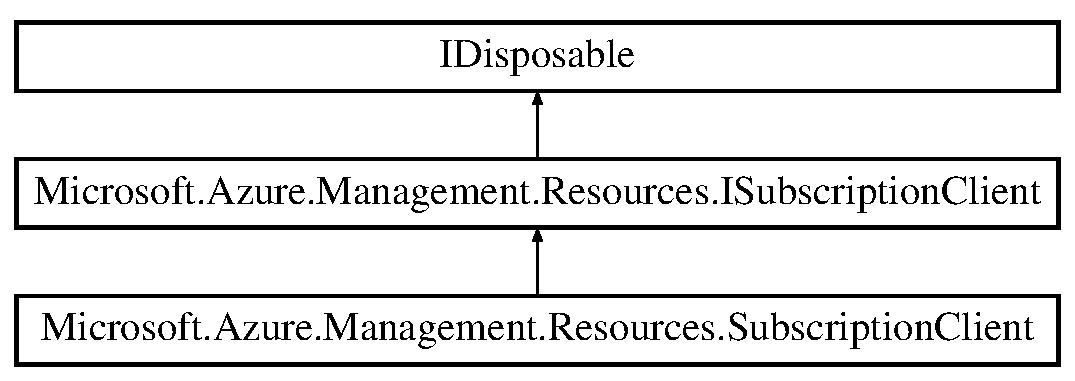
\includegraphics[height=3.000000cm]{interface_microsoft_1_1_azure_1_1_management_1_1_resources_1_1_i_subscription_client}
\end{center}
\end{figure}
\subsection*{Properties}
\begin{DoxyCompactItemize}
\item 
Uri \hyperlink{interface_microsoft_1_1_azure_1_1_management_1_1_resources_1_1_i_subscription_client_a22e5d877b02ff30230be0b5541cdd7a1}{Base\+Uri}\hspace{0.3cm}{\ttfamily  \mbox{[}get, set\mbox{]}}
\begin{DoxyCompactList}\small\item\em The base U\+RI of the service. \end{DoxyCompactList}\item 
Json\+Serializer\+Settings \hyperlink{interface_microsoft_1_1_azure_1_1_management_1_1_resources_1_1_i_subscription_client_a56b59fb47022a9b49b4ee3e828d2d070}{Serialization\+Settings}\hspace{0.3cm}{\ttfamily  \mbox{[}get\mbox{]}}
\begin{DoxyCompactList}\small\item\em Gets or sets json serialization settings. \end{DoxyCompactList}\item 
Json\+Serializer\+Settings \hyperlink{interface_microsoft_1_1_azure_1_1_management_1_1_resources_1_1_i_subscription_client_a9043d6bb08b8f55b779b4038f36102da}{Deserialization\+Settings}\hspace{0.3cm}{\ttfamily  \mbox{[}get\mbox{]}}
\begin{DoxyCompactList}\small\item\em Gets or sets json deserialization settings. \end{DoxyCompactList}\item 
Service\+Client\+Credentials \hyperlink{interface_microsoft_1_1_azure_1_1_management_1_1_resources_1_1_i_subscription_client_a77f1f5d7013d3b987c0ce72384f77d08}{Credentials}\hspace{0.3cm}{\ttfamily  \mbox{[}get\mbox{]}}
\begin{DoxyCompactList}\small\item\em The management credentials for \hyperlink{namespace_microsoft_1_1_azure}{Azure}. \end{DoxyCompactList}\item 
string \hyperlink{interface_microsoft_1_1_azure_1_1_management_1_1_resources_1_1_i_subscription_client_aa7170040fe7cc8a8c209ae6857a54cbf}{Subscription\+Id}\hspace{0.3cm}{\ttfamily  \mbox{[}get, set\mbox{]}}
\begin{DoxyCompactList}\small\item\em Gets subscription credentials which uniquely identify \hyperlink{namespace_microsoft}{Microsoft} \hyperlink{namespace_microsoft_1_1_azure}{Azure} subscription. The subscription ID forms part of the U\+RI for every service call. \end{DoxyCompactList}\item 
string \hyperlink{interface_microsoft_1_1_azure_1_1_management_1_1_resources_1_1_i_subscription_client_a5145743b1565db5907a4f553cea767d8}{Api\+Version}\hspace{0.3cm}{\ttfamily  \mbox{[}get\mbox{]}}
\begin{DoxyCompactList}\small\item\em Client Api Version. \end{DoxyCompactList}\item 
string \hyperlink{interface_microsoft_1_1_azure_1_1_management_1_1_resources_1_1_i_subscription_client_a30bf8817047a3b3a860004dd1bfd611f}{Accept\+Language}\hspace{0.3cm}{\ttfamily  \mbox{[}get, set\mbox{]}}
\begin{DoxyCompactList}\small\item\em Gets or sets the preferred language for the response. \end{DoxyCompactList}\item 
int \hyperlink{interface_microsoft_1_1_azure_1_1_management_1_1_resources_1_1_i_subscription_client_a8e15418fd4134bc377566d9215151a4a}{Long\+Running\+Operation\+Retry\+Timeout}\hspace{0.3cm}{\ttfamily  \mbox{[}get, set\mbox{]}}
\begin{DoxyCompactList}\small\item\em The retry timeout for Long Running Operations. \end{DoxyCompactList}\item 
\hyperlink{interface_microsoft_1_1_azure_1_1_management_1_1_resources_1_1_i_subscriptions_operations}{I\+Subscriptions\+Operations} {\bfseries Subscriptions}\hspace{0.3cm}{\ttfamily  \mbox{[}get\mbox{]}}\hypertarget{interface_microsoft_1_1_azure_1_1_management_1_1_resources_1_1_i_subscription_client_a0bc138534690e37ca9390b56916098d0}{}\label{interface_microsoft_1_1_azure_1_1_management_1_1_resources_1_1_i_subscription_client_a0bc138534690e37ca9390b56916098d0}

\item 
\hyperlink{interface_microsoft_1_1_azure_1_1_management_1_1_resources_1_1_i_tenants_operations}{I\+Tenants\+Operations} {\bfseries Tenants}\hspace{0.3cm}{\ttfamily  \mbox{[}get\mbox{]}}\hypertarget{interface_microsoft_1_1_azure_1_1_management_1_1_resources_1_1_i_subscription_client_a73ffb246548d9f167b1f04e5039d7237}{}\label{interface_microsoft_1_1_azure_1_1_management_1_1_resources_1_1_i_subscription_client_a73ffb246548d9f167b1f04e5039d7237}

\end{DoxyCompactItemize}


\subsection{Detailed Description}




\subsection{Property Documentation}
\index{Microsoft\+::\+Azure\+::\+Management\+::\+Resources\+::\+I\+Subscription\+Client@{Microsoft\+::\+Azure\+::\+Management\+::\+Resources\+::\+I\+Subscription\+Client}!Accept\+Language@{Accept\+Language}}
\index{Accept\+Language@{Accept\+Language}!Microsoft\+::\+Azure\+::\+Management\+::\+Resources\+::\+I\+Subscription\+Client@{Microsoft\+::\+Azure\+::\+Management\+::\+Resources\+::\+I\+Subscription\+Client}}
\subsubsection[{\texorpdfstring{Accept\+Language}{AcceptLanguage}}]{\setlength{\rightskip}{0pt plus 5cm}string Microsoft.\+Azure.\+Management.\+Resources.\+I\+Subscription\+Client.\+Accept\+Language\hspace{0.3cm}{\ttfamily [get]}, {\ttfamily [set]}}\hypertarget{interface_microsoft_1_1_azure_1_1_management_1_1_resources_1_1_i_subscription_client_a30bf8817047a3b3a860004dd1bfd611f}{}\label{interface_microsoft_1_1_azure_1_1_management_1_1_resources_1_1_i_subscription_client_a30bf8817047a3b3a860004dd1bfd611f}


Gets or sets the preferred language for the response. 

\index{Microsoft\+::\+Azure\+::\+Management\+::\+Resources\+::\+I\+Subscription\+Client@{Microsoft\+::\+Azure\+::\+Management\+::\+Resources\+::\+I\+Subscription\+Client}!Api\+Version@{Api\+Version}}
\index{Api\+Version@{Api\+Version}!Microsoft\+::\+Azure\+::\+Management\+::\+Resources\+::\+I\+Subscription\+Client@{Microsoft\+::\+Azure\+::\+Management\+::\+Resources\+::\+I\+Subscription\+Client}}
\subsubsection[{\texorpdfstring{Api\+Version}{ApiVersion}}]{\setlength{\rightskip}{0pt plus 5cm}string Microsoft.\+Azure.\+Management.\+Resources.\+I\+Subscription\+Client.\+Api\+Version\hspace{0.3cm}{\ttfamily [get]}}\hypertarget{interface_microsoft_1_1_azure_1_1_management_1_1_resources_1_1_i_subscription_client_a5145743b1565db5907a4f553cea767d8}{}\label{interface_microsoft_1_1_azure_1_1_management_1_1_resources_1_1_i_subscription_client_a5145743b1565db5907a4f553cea767d8}


Client Api Version. 

\index{Microsoft\+::\+Azure\+::\+Management\+::\+Resources\+::\+I\+Subscription\+Client@{Microsoft\+::\+Azure\+::\+Management\+::\+Resources\+::\+I\+Subscription\+Client}!Base\+Uri@{Base\+Uri}}
\index{Base\+Uri@{Base\+Uri}!Microsoft\+::\+Azure\+::\+Management\+::\+Resources\+::\+I\+Subscription\+Client@{Microsoft\+::\+Azure\+::\+Management\+::\+Resources\+::\+I\+Subscription\+Client}}
\subsubsection[{\texorpdfstring{Base\+Uri}{BaseUri}}]{\setlength{\rightskip}{0pt plus 5cm}Uri Microsoft.\+Azure.\+Management.\+Resources.\+I\+Subscription\+Client.\+Base\+Uri\hspace{0.3cm}{\ttfamily [get]}, {\ttfamily [set]}}\hypertarget{interface_microsoft_1_1_azure_1_1_management_1_1_resources_1_1_i_subscription_client_a22e5d877b02ff30230be0b5541cdd7a1}{}\label{interface_microsoft_1_1_azure_1_1_management_1_1_resources_1_1_i_subscription_client_a22e5d877b02ff30230be0b5541cdd7a1}


The base U\+RI of the service. 

\index{Microsoft\+::\+Azure\+::\+Management\+::\+Resources\+::\+I\+Subscription\+Client@{Microsoft\+::\+Azure\+::\+Management\+::\+Resources\+::\+I\+Subscription\+Client}!Credentials@{Credentials}}
\index{Credentials@{Credentials}!Microsoft\+::\+Azure\+::\+Management\+::\+Resources\+::\+I\+Subscription\+Client@{Microsoft\+::\+Azure\+::\+Management\+::\+Resources\+::\+I\+Subscription\+Client}}
\subsubsection[{\texorpdfstring{Credentials}{Credentials}}]{\setlength{\rightskip}{0pt plus 5cm}Service\+Client\+Credentials Microsoft.\+Azure.\+Management.\+Resources.\+I\+Subscription\+Client.\+Credentials\hspace{0.3cm}{\ttfamily [get]}}\hypertarget{interface_microsoft_1_1_azure_1_1_management_1_1_resources_1_1_i_subscription_client_a77f1f5d7013d3b987c0ce72384f77d08}{}\label{interface_microsoft_1_1_azure_1_1_management_1_1_resources_1_1_i_subscription_client_a77f1f5d7013d3b987c0ce72384f77d08}


The management credentials for \hyperlink{namespace_microsoft_1_1_azure}{Azure}. 

\index{Microsoft\+::\+Azure\+::\+Management\+::\+Resources\+::\+I\+Subscription\+Client@{Microsoft\+::\+Azure\+::\+Management\+::\+Resources\+::\+I\+Subscription\+Client}!Deserialization\+Settings@{Deserialization\+Settings}}
\index{Deserialization\+Settings@{Deserialization\+Settings}!Microsoft\+::\+Azure\+::\+Management\+::\+Resources\+::\+I\+Subscription\+Client@{Microsoft\+::\+Azure\+::\+Management\+::\+Resources\+::\+I\+Subscription\+Client}}
\subsubsection[{\texorpdfstring{Deserialization\+Settings}{DeserializationSettings}}]{\setlength{\rightskip}{0pt plus 5cm}Json\+Serializer\+Settings Microsoft.\+Azure.\+Management.\+Resources.\+I\+Subscription\+Client.\+Deserialization\+Settings\hspace{0.3cm}{\ttfamily [get]}}\hypertarget{interface_microsoft_1_1_azure_1_1_management_1_1_resources_1_1_i_subscription_client_a9043d6bb08b8f55b779b4038f36102da}{}\label{interface_microsoft_1_1_azure_1_1_management_1_1_resources_1_1_i_subscription_client_a9043d6bb08b8f55b779b4038f36102da}


Gets or sets json deserialization settings. 

\index{Microsoft\+::\+Azure\+::\+Management\+::\+Resources\+::\+I\+Subscription\+Client@{Microsoft\+::\+Azure\+::\+Management\+::\+Resources\+::\+I\+Subscription\+Client}!Long\+Running\+Operation\+Retry\+Timeout@{Long\+Running\+Operation\+Retry\+Timeout}}
\index{Long\+Running\+Operation\+Retry\+Timeout@{Long\+Running\+Operation\+Retry\+Timeout}!Microsoft\+::\+Azure\+::\+Management\+::\+Resources\+::\+I\+Subscription\+Client@{Microsoft\+::\+Azure\+::\+Management\+::\+Resources\+::\+I\+Subscription\+Client}}
\subsubsection[{\texorpdfstring{Long\+Running\+Operation\+Retry\+Timeout}{LongRunningOperationRetryTimeout}}]{\setlength{\rightskip}{0pt plus 5cm}int Microsoft.\+Azure.\+Management.\+Resources.\+I\+Subscription\+Client.\+Long\+Running\+Operation\+Retry\+Timeout\hspace{0.3cm}{\ttfamily [get]}, {\ttfamily [set]}}\hypertarget{interface_microsoft_1_1_azure_1_1_management_1_1_resources_1_1_i_subscription_client_a8e15418fd4134bc377566d9215151a4a}{}\label{interface_microsoft_1_1_azure_1_1_management_1_1_resources_1_1_i_subscription_client_a8e15418fd4134bc377566d9215151a4a}


The retry timeout for Long Running Operations. 

\index{Microsoft\+::\+Azure\+::\+Management\+::\+Resources\+::\+I\+Subscription\+Client@{Microsoft\+::\+Azure\+::\+Management\+::\+Resources\+::\+I\+Subscription\+Client}!Serialization\+Settings@{Serialization\+Settings}}
\index{Serialization\+Settings@{Serialization\+Settings}!Microsoft\+::\+Azure\+::\+Management\+::\+Resources\+::\+I\+Subscription\+Client@{Microsoft\+::\+Azure\+::\+Management\+::\+Resources\+::\+I\+Subscription\+Client}}
\subsubsection[{\texorpdfstring{Serialization\+Settings}{SerializationSettings}}]{\setlength{\rightskip}{0pt plus 5cm}Json\+Serializer\+Settings Microsoft.\+Azure.\+Management.\+Resources.\+I\+Subscription\+Client.\+Serialization\+Settings\hspace{0.3cm}{\ttfamily [get]}}\hypertarget{interface_microsoft_1_1_azure_1_1_management_1_1_resources_1_1_i_subscription_client_a56b59fb47022a9b49b4ee3e828d2d070}{}\label{interface_microsoft_1_1_azure_1_1_management_1_1_resources_1_1_i_subscription_client_a56b59fb47022a9b49b4ee3e828d2d070}


Gets or sets json serialization settings. 

\index{Microsoft\+::\+Azure\+::\+Management\+::\+Resources\+::\+I\+Subscription\+Client@{Microsoft\+::\+Azure\+::\+Management\+::\+Resources\+::\+I\+Subscription\+Client}!Subscription\+Id@{Subscription\+Id}}
\index{Subscription\+Id@{Subscription\+Id}!Microsoft\+::\+Azure\+::\+Management\+::\+Resources\+::\+I\+Subscription\+Client@{Microsoft\+::\+Azure\+::\+Management\+::\+Resources\+::\+I\+Subscription\+Client}}
\subsubsection[{\texorpdfstring{Subscription\+Id}{SubscriptionId}}]{\setlength{\rightskip}{0pt plus 5cm}string Microsoft.\+Azure.\+Management.\+Resources.\+I\+Subscription\+Client.\+Subscription\+Id\hspace{0.3cm}{\ttfamily [get]}, {\ttfamily [set]}}\hypertarget{interface_microsoft_1_1_azure_1_1_management_1_1_resources_1_1_i_subscription_client_aa7170040fe7cc8a8c209ae6857a54cbf}{}\label{interface_microsoft_1_1_azure_1_1_management_1_1_resources_1_1_i_subscription_client_aa7170040fe7cc8a8c209ae6857a54cbf}


Gets subscription credentials which uniquely identify \hyperlink{namespace_microsoft}{Microsoft} \hyperlink{namespace_microsoft_1_1_azure}{Azure} subscription. The subscription ID forms part of the U\+RI for every service call. 



The documentation for this interface was generated from the following file\+:\begin{DoxyCompactItemize}
\item 
files/I\+Subscription\+Client.\+cs\end{DoxyCompactItemize}

\hypertarget{interface_microsoft_1_1_azure_1_1_management_1_1_resources_1_1_i_subscriptions_operations}{}\section{Microsoft.\+Azure.\+Management.\+Resources.\+I\+Subscriptions\+Operations Interface Reference}
\label{interface_microsoft_1_1_azure_1_1_management_1_1_resources_1_1_i_subscriptions_operations}\index{Microsoft.\+Azure.\+Management.\+Resources.\+I\+Subscriptions\+Operations@{Microsoft.\+Azure.\+Management.\+Resources.\+I\+Subscriptions\+Operations}}


Subscriptions\+Operations operations.  




Inherited by Microsoft.\+Azure.\+Management.\+Resources.\+Subscriptions\+Operations.

\subsection*{Public Member Functions}
\begin{DoxyCompactItemize}
\item 
Task$<$ Azure\+Operation\+Response$<$ I\+Page$<$ Location $>$ $>$ $>$ \hyperlink{interface_microsoft_1_1_azure_1_1_management_1_1_resources_1_1_i_subscriptions_operations_ab64606da41b4c013a6d0120325aa245e}{List\+Locations\+With\+Http\+Messages\+Async} (string subscription\+Id, Dictionary$<$ string, List$<$ string $>$$>$ custom\+Headers=null, Cancellation\+Token cancellation\+Token=default(Cancellation\+Token))
\begin{DoxyCompactList}\small\item\em Gets a list of the subscription locations. \end{DoxyCompactList}\item 
Task$<$ Azure\+Operation\+Response$<$ Subscription $>$ $>$ \hyperlink{interface_microsoft_1_1_azure_1_1_management_1_1_resources_1_1_i_subscriptions_operations_a6b8613944f5cf5995f100bcfb7d4ba2a}{Get\+With\+Http\+Messages\+Async} (string subscription\+Id, Dictionary$<$ string, List$<$ string $>$$>$ custom\+Headers=null, Cancellation\+Token cancellation\+Token=default(Cancellation\+Token))
\begin{DoxyCompactList}\small\item\em Gets details about particular subscription. \end{DoxyCompactList}\item 
Task$<$ Azure\+Operation\+Response$<$ I\+Page$<$ Subscription $>$ $>$ $>$ \hyperlink{interface_microsoft_1_1_azure_1_1_management_1_1_resources_1_1_i_subscriptions_operations_a33722bd0f5485e9196e1242ad521c40b}{List\+With\+Http\+Messages\+Async} (Dictionary$<$ string, List$<$ string $>$$>$ custom\+Headers=null, Cancellation\+Token cancellation\+Token=default(Cancellation\+Token))
\begin{DoxyCompactList}\small\item\em Gets a list of the subscription\+Ids. \end{DoxyCompactList}\item 
Task$<$ Azure\+Operation\+Response$<$ I\+Page$<$ Location $>$ $>$ $>$ \hyperlink{interface_microsoft_1_1_azure_1_1_management_1_1_resources_1_1_i_subscriptions_operations_a972e2f414754d9996c40536420329e02}{List\+Locations\+Next\+With\+Http\+Messages\+Async} (string next\+Page\+Link, Dictionary$<$ string, List$<$ string $>$$>$ custom\+Headers=null, Cancellation\+Token cancellation\+Token=default(Cancellation\+Token))
\begin{DoxyCompactList}\small\item\em Gets a list of the subscription locations. \end{DoxyCompactList}\item 
Task$<$ Azure\+Operation\+Response$<$ I\+Page$<$ Subscription $>$ $>$ $>$ \hyperlink{interface_microsoft_1_1_azure_1_1_management_1_1_resources_1_1_i_subscriptions_operations_aa7c289b12146484dbb129e5533cd6c36}{List\+Next\+With\+Http\+Messages\+Async} (string next\+Page\+Link, Dictionary$<$ string, List$<$ string $>$$>$ custom\+Headers=null, Cancellation\+Token cancellation\+Token=default(Cancellation\+Token))
\begin{DoxyCompactList}\small\item\em Gets a list of the subscription\+Ids. \end{DoxyCompactList}\end{DoxyCompactItemize}


\subsection{Detailed Description}
Subscriptions\+Operations operations. 



\subsection{Member Function Documentation}
\index{Microsoft\+::\+Azure\+::\+Management\+::\+Resources\+::\+I\+Subscriptions\+Operations@{Microsoft\+::\+Azure\+::\+Management\+::\+Resources\+::\+I\+Subscriptions\+Operations}!Get\+With\+Http\+Messages\+Async@{Get\+With\+Http\+Messages\+Async}}
\index{Get\+With\+Http\+Messages\+Async@{Get\+With\+Http\+Messages\+Async}!Microsoft\+::\+Azure\+::\+Management\+::\+Resources\+::\+I\+Subscriptions\+Operations@{Microsoft\+::\+Azure\+::\+Management\+::\+Resources\+::\+I\+Subscriptions\+Operations}}
\subsubsection[{\texorpdfstring{Get\+With\+Http\+Messages\+Async(string subscription\+Id, Dictionary$<$ string, List$<$ string $>$$>$ custom\+Headers=null, Cancellation\+Token cancellation\+Token=default(\+Cancellation\+Token))}{GetWithHttpMessagesAsync(string subscriptionId, Dictionary< string, List< string >> customHeaders=null, CancellationToken cancellationToken=default(CancellationToken))}}]{\setlength{\rightskip}{0pt plus 5cm}Task$<$Azure\+Operation\+Response$<$Subscription$>$ $>$ Microsoft.\+Azure.\+Management.\+Resources.\+I\+Subscriptions\+Operations.\+Get\+With\+Http\+Messages\+Async (
\begin{DoxyParamCaption}
\item[{string}]{subscription\+Id, }
\item[{Dictionary$<$ string, List$<$ string $>$$>$}]{custom\+Headers = {\ttfamily null}, }
\item[{Cancellation\+Token}]{cancellation\+Token = {\ttfamily default(CancellationToken)}}
\end{DoxyParamCaption}
)}\hypertarget{interface_microsoft_1_1_azure_1_1_management_1_1_resources_1_1_i_subscriptions_operations_a6b8613944f5cf5995f100bcfb7d4ba2a}{}\label{interface_microsoft_1_1_azure_1_1_management_1_1_resources_1_1_i_subscriptions_operations_a6b8613944f5cf5995f100bcfb7d4ba2a}


Gets details about particular subscription. 


\begin{DoxyParams}{Parameters}
{\em subscription\+Id} & Id of the subscription. \\
\hline
{\em custom\+Headers} & The headers that will be added to request. \\
\hline
{\em cancellation\+Token} & The cancellation token. \\
\hline
\end{DoxyParams}
\index{Microsoft\+::\+Azure\+::\+Management\+::\+Resources\+::\+I\+Subscriptions\+Operations@{Microsoft\+::\+Azure\+::\+Management\+::\+Resources\+::\+I\+Subscriptions\+Operations}!List\+Locations\+Next\+With\+Http\+Messages\+Async@{List\+Locations\+Next\+With\+Http\+Messages\+Async}}
\index{List\+Locations\+Next\+With\+Http\+Messages\+Async@{List\+Locations\+Next\+With\+Http\+Messages\+Async}!Microsoft\+::\+Azure\+::\+Management\+::\+Resources\+::\+I\+Subscriptions\+Operations@{Microsoft\+::\+Azure\+::\+Management\+::\+Resources\+::\+I\+Subscriptions\+Operations}}
\subsubsection[{\texorpdfstring{List\+Locations\+Next\+With\+Http\+Messages\+Async(string next\+Page\+Link, Dictionary$<$ string, List$<$ string $>$$>$ custom\+Headers=null, Cancellation\+Token cancellation\+Token=default(\+Cancellation\+Token))}{ListLocationsNextWithHttpMessagesAsync(string nextPageLink, Dictionary< string, List< string >> customHeaders=null, CancellationToken cancellationToken=default(CancellationToken))}}]{\setlength{\rightskip}{0pt plus 5cm}Task$<$Azure\+Operation\+Response$<$I\+Page$<$Location$>$ $>$ $>$ Microsoft.\+Azure.\+Management.\+Resources.\+I\+Subscriptions\+Operations.\+List\+Locations\+Next\+With\+Http\+Messages\+Async (
\begin{DoxyParamCaption}
\item[{string}]{next\+Page\+Link, }
\item[{Dictionary$<$ string, List$<$ string $>$$>$}]{custom\+Headers = {\ttfamily null}, }
\item[{Cancellation\+Token}]{cancellation\+Token = {\ttfamily default(CancellationToken)}}
\end{DoxyParamCaption}
)}\hypertarget{interface_microsoft_1_1_azure_1_1_management_1_1_resources_1_1_i_subscriptions_operations_a972e2f414754d9996c40536420329e02}{}\label{interface_microsoft_1_1_azure_1_1_management_1_1_resources_1_1_i_subscriptions_operations_a972e2f414754d9996c40536420329e02}


Gets a list of the subscription locations. 


\begin{DoxyParams}{Parameters}
{\em next\+Page\+Link} & The Next\+Link from the previous successful call to List operation. \\
\hline
{\em custom\+Headers} & The headers that will be added to request. \\
\hline
{\em cancellation\+Token} & The cancellation token. \\
\hline
\end{DoxyParams}
\index{Microsoft\+::\+Azure\+::\+Management\+::\+Resources\+::\+I\+Subscriptions\+Operations@{Microsoft\+::\+Azure\+::\+Management\+::\+Resources\+::\+I\+Subscriptions\+Operations}!List\+Locations\+With\+Http\+Messages\+Async@{List\+Locations\+With\+Http\+Messages\+Async}}
\index{List\+Locations\+With\+Http\+Messages\+Async@{List\+Locations\+With\+Http\+Messages\+Async}!Microsoft\+::\+Azure\+::\+Management\+::\+Resources\+::\+I\+Subscriptions\+Operations@{Microsoft\+::\+Azure\+::\+Management\+::\+Resources\+::\+I\+Subscriptions\+Operations}}
\subsubsection[{\texorpdfstring{List\+Locations\+With\+Http\+Messages\+Async(string subscription\+Id, Dictionary$<$ string, List$<$ string $>$$>$ custom\+Headers=null, Cancellation\+Token cancellation\+Token=default(\+Cancellation\+Token))}{ListLocationsWithHttpMessagesAsync(string subscriptionId, Dictionary< string, List< string >> customHeaders=null, CancellationToken cancellationToken=default(CancellationToken))}}]{\setlength{\rightskip}{0pt plus 5cm}Task$<$Azure\+Operation\+Response$<$I\+Page$<$Location$>$ $>$ $>$ Microsoft.\+Azure.\+Management.\+Resources.\+I\+Subscriptions\+Operations.\+List\+Locations\+With\+Http\+Messages\+Async (
\begin{DoxyParamCaption}
\item[{string}]{subscription\+Id, }
\item[{Dictionary$<$ string, List$<$ string $>$$>$}]{custom\+Headers = {\ttfamily null}, }
\item[{Cancellation\+Token}]{cancellation\+Token = {\ttfamily default(CancellationToken)}}
\end{DoxyParamCaption}
)}\hypertarget{interface_microsoft_1_1_azure_1_1_management_1_1_resources_1_1_i_subscriptions_operations_ab64606da41b4c013a6d0120325aa245e}{}\label{interface_microsoft_1_1_azure_1_1_management_1_1_resources_1_1_i_subscriptions_operations_ab64606da41b4c013a6d0120325aa245e}


Gets a list of the subscription locations. 


\begin{DoxyParams}{Parameters}
{\em subscription\+Id} & Id of the subscription \\
\hline
{\em custom\+Headers} & The headers that will be added to request. \\
\hline
{\em cancellation\+Token} & The cancellation token. \\
\hline
\end{DoxyParams}
\index{Microsoft\+::\+Azure\+::\+Management\+::\+Resources\+::\+I\+Subscriptions\+Operations@{Microsoft\+::\+Azure\+::\+Management\+::\+Resources\+::\+I\+Subscriptions\+Operations}!List\+Next\+With\+Http\+Messages\+Async@{List\+Next\+With\+Http\+Messages\+Async}}
\index{List\+Next\+With\+Http\+Messages\+Async@{List\+Next\+With\+Http\+Messages\+Async}!Microsoft\+::\+Azure\+::\+Management\+::\+Resources\+::\+I\+Subscriptions\+Operations@{Microsoft\+::\+Azure\+::\+Management\+::\+Resources\+::\+I\+Subscriptions\+Operations}}
\subsubsection[{\texorpdfstring{List\+Next\+With\+Http\+Messages\+Async(string next\+Page\+Link, Dictionary$<$ string, List$<$ string $>$$>$ custom\+Headers=null, Cancellation\+Token cancellation\+Token=default(\+Cancellation\+Token))}{ListNextWithHttpMessagesAsync(string nextPageLink, Dictionary< string, List< string >> customHeaders=null, CancellationToken cancellationToken=default(CancellationToken))}}]{\setlength{\rightskip}{0pt plus 5cm}Task$<$Azure\+Operation\+Response$<$I\+Page$<$Subscription$>$ $>$ $>$ Microsoft.\+Azure.\+Management.\+Resources.\+I\+Subscriptions\+Operations.\+List\+Next\+With\+Http\+Messages\+Async (
\begin{DoxyParamCaption}
\item[{string}]{next\+Page\+Link, }
\item[{Dictionary$<$ string, List$<$ string $>$$>$}]{custom\+Headers = {\ttfamily null}, }
\item[{Cancellation\+Token}]{cancellation\+Token = {\ttfamily default(CancellationToken)}}
\end{DoxyParamCaption}
)}\hypertarget{interface_microsoft_1_1_azure_1_1_management_1_1_resources_1_1_i_subscriptions_operations_aa7c289b12146484dbb129e5533cd6c36}{}\label{interface_microsoft_1_1_azure_1_1_management_1_1_resources_1_1_i_subscriptions_operations_aa7c289b12146484dbb129e5533cd6c36}


Gets a list of the subscription\+Ids. 


\begin{DoxyParams}{Parameters}
{\em next\+Page\+Link} & The Next\+Link from the previous successful call to List operation. \\
\hline
{\em custom\+Headers} & The headers that will be added to request. \\
\hline
{\em cancellation\+Token} & The cancellation token. \\
\hline
\end{DoxyParams}
\index{Microsoft\+::\+Azure\+::\+Management\+::\+Resources\+::\+I\+Subscriptions\+Operations@{Microsoft\+::\+Azure\+::\+Management\+::\+Resources\+::\+I\+Subscriptions\+Operations}!List\+With\+Http\+Messages\+Async@{List\+With\+Http\+Messages\+Async}}
\index{List\+With\+Http\+Messages\+Async@{List\+With\+Http\+Messages\+Async}!Microsoft\+::\+Azure\+::\+Management\+::\+Resources\+::\+I\+Subscriptions\+Operations@{Microsoft\+::\+Azure\+::\+Management\+::\+Resources\+::\+I\+Subscriptions\+Operations}}
\subsubsection[{\texorpdfstring{List\+With\+Http\+Messages\+Async(\+Dictionary$<$ string, List$<$ string $>$$>$ custom\+Headers=null, Cancellation\+Token cancellation\+Token=default(\+Cancellation\+Token))}{ListWithHttpMessagesAsync(Dictionary< string, List< string >> customHeaders=null, CancellationToken cancellationToken=default(CancellationToken))}}]{\setlength{\rightskip}{0pt plus 5cm}Task$<$Azure\+Operation\+Response$<$I\+Page$<$Subscription$>$ $>$ $>$ Microsoft.\+Azure.\+Management.\+Resources.\+I\+Subscriptions\+Operations.\+List\+With\+Http\+Messages\+Async (
\begin{DoxyParamCaption}
\item[{Dictionary$<$ string, List$<$ string $>$$>$}]{custom\+Headers = {\ttfamily null}, }
\item[{Cancellation\+Token}]{cancellation\+Token = {\ttfamily default(CancellationToken)}}
\end{DoxyParamCaption}
)}\hypertarget{interface_microsoft_1_1_azure_1_1_management_1_1_resources_1_1_i_subscriptions_operations_a33722bd0f5485e9196e1242ad521c40b}{}\label{interface_microsoft_1_1_azure_1_1_management_1_1_resources_1_1_i_subscriptions_operations_a33722bd0f5485e9196e1242ad521c40b}


Gets a list of the subscription\+Ids. 


\begin{DoxyParams}{Parameters}
{\em custom\+Headers} & The headers that will be added to request. \\
\hline
{\em cancellation\+Token} & The cancellation token. \\
\hline
\end{DoxyParams}


The documentation for this interface was generated from the following file\+:\begin{DoxyCompactItemize}
\item 
files/I\+Subscriptions\+Operations.\+cs\end{DoxyCompactItemize}

\hypertarget{interface_microsoft_1_1_azure_1_1_management_1_1_resources_1_1_i_tags_operations}{}\section{Microsoft.\+Azure.\+Management.\+Resources.\+I\+Tags\+Operations Interface Reference}
\label{interface_microsoft_1_1_azure_1_1_management_1_1_resources_1_1_i_tags_operations}\index{Microsoft.\+Azure.\+Management.\+Resources.\+I\+Tags\+Operations@{Microsoft.\+Azure.\+Management.\+Resources.\+I\+Tags\+Operations}}


Tags\+Operations operations.  




Inherited by Microsoft.\+Azure.\+Management.\+Resources.\+Tags\+Operations.

\subsection*{Public Member Functions}
\begin{DoxyCompactItemize}
\item 
Task$<$ Azure\+Operation\+Response $>$ \hyperlink{interface_microsoft_1_1_azure_1_1_management_1_1_resources_1_1_i_tags_operations_af81287296804575ba94fde7d4f8dedb5}{Delete\+Value\+With\+Http\+Messages\+Async} (string tag\+Name, string tag\+Value, Dictionary$<$ string, List$<$ string $>$$>$ custom\+Headers=null, Cancellation\+Token cancellation\+Token=default(Cancellation\+Token))
\begin{DoxyCompactList}\small\item\em Delete a subscription resource tag value. \end{DoxyCompactList}\item 
Task$<$ Azure\+Operation\+Response$<$ Tag\+Value $>$ $>$ \hyperlink{interface_microsoft_1_1_azure_1_1_management_1_1_resources_1_1_i_tags_operations_a892e47052346b06887bd32b1d6621586}{Create\+Or\+Update\+Value\+With\+Http\+Messages\+Async} (string tag\+Name, string tag\+Value, Dictionary$<$ string, List$<$ string $>$$>$ custom\+Headers=null, Cancellation\+Token cancellation\+Token=default(Cancellation\+Token))
\begin{DoxyCompactList}\small\item\em Create a subscription resource tag value. \end{DoxyCompactList}\item 
Task$<$ Azure\+Operation\+Response$<$ Tag\+Details $>$ $>$ \hyperlink{interface_microsoft_1_1_azure_1_1_management_1_1_resources_1_1_i_tags_operations_a74b501c4f8456cca99f81f809a1318ed}{Create\+Or\+Update\+With\+Http\+Messages\+Async} (string tag\+Name, Dictionary$<$ string, List$<$ string $>$$>$ custom\+Headers=null, Cancellation\+Token cancellation\+Token=default(Cancellation\+Token))
\begin{DoxyCompactList}\small\item\em Create a subscription resource tag. \end{DoxyCompactList}\item 
Task$<$ Azure\+Operation\+Response $>$ \hyperlink{interface_microsoft_1_1_azure_1_1_management_1_1_resources_1_1_i_tags_operations_acc4ec733e871cbd290ea653dc904aeae}{Delete\+With\+Http\+Messages\+Async} (string tag\+Name, Dictionary$<$ string, List$<$ string $>$$>$ custom\+Headers=null, Cancellation\+Token cancellation\+Token=default(Cancellation\+Token))
\begin{DoxyCompactList}\small\item\em Delete a subscription resource tag. \end{DoxyCompactList}\item 
Task$<$ Azure\+Operation\+Response$<$ I\+Page$<$ Tag\+Details $>$ $>$ $>$ \hyperlink{interface_microsoft_1_1_azure_1_1_management_1_1_resources_1_1_i_tags_operations_ad2b5bccc8638da0b9964676db6b858e6}{List\+With\+Http\+Messages\+Async} (Dictionary$<$ string, List$<$ string $>$$>$ custom\+Headers=null, Cancellation\+Token cancellation\+Token=default(Cancellation\+Token))
\begin{DoxyCompactList}\small\item\em Get a list of subscription resource tags. \end{DoxyCompactList}\item 
Task$<$ Azure\+Operation\+Response$<$ I\+Page$<$ Tag\+Details $>$ $>$ $>$ \hyperlink{interface_microsoft_1_1_azure_1_1_management_1_1_resources_1_1_i_tags_operations_a2b5f25361f8e34269c9f298e10170b76}{List\+Next\+With\+Http\+Messages\+Async} (string next\+Page\+Link, Dictionary$<$ string, List$<$ string $>$$>$ custom\+Headers=null, Cancellation\+Token cancellation\+Token=default(Cancellation\+Token))
\begin{DoxyCompactList}\small\item\em Get a list of subscription resource tags. \end{DoxyCompactList}\end{DoxyCompactItemize}


\subsection{Detailed Description}
Tags\+Operations operations. 



\subsection{Member Function Documentation}
\index{Microsoft\+::\+Azure\+::\+Management\+::\+Resources\+::\+I\+Tags\+Operations@{Microsoft\+::\+Azure\+::\+Management\+::\+Resources\+::\+I\+Tags\+Operations}!Create\+Or\+Update\+Value\+With\+Http\+Messages\+Async@{Create\+Or\+Update\+Value\+With\+Http\+Messages\+Async}}
\index{Create\+Or\+Update\+Value\+With\+Http\+Messages\+Async@{Create\+Or\+Update\+Value\+With\+Http\+Messages\+Async}!Microsoft\+::\+Azure\+::\+Management\+::\+Resources\+::\+I\+Tags\+Operations@{Microsoft\+::\+Azure\+::\+Management\+::\+Resources\+::\+I\+Tags\+Operations}}
\subsubsection[{\texorpdfstring{Create\+Or\+Update\+Value\+With\+Http\+Messages\+Async(string tag\+Name, string tag\+Value, Dictionary$<$ string, List$<$ string $>$$>$ custom\+Headers=null, Cancellation\+Token cancellation\+Token=default(\+Cancellation\+Token))}{CreateOrUpdateValueWithHttpMessagesAsync(string tagName, string tagValue, Dictionary< string, List< string >> customHeaders=null, CancellationToken cancellationToken=default(CancellationToken))}}]{\setlength{\rightskip}{0pt plus 5cm}Task$<$Azure\+Operation\+Response$<$Tag\+Value$>$ $>$ Microsoft.\+Azure.\+Management.\+Resources.\+I\+Tags\+Operations.\+Create\+Or\+Update\+Value\+With\+Http\+Messages\+Async (
\begin{DoxyParamCaption}
\item[{string}]{tag\+Name, }
\item[{string}]{tag\+Value, }
\item[{Dictionary$<$ string, List$<$ string $>$$>$}]{custom\+Headers = {\ttfamily null}, }
\item[{Cancellation\+Token}]{cancellation\+Token = {\ttfamily default(CancellationToken)}}
\end{DoxyParamCaption}
)}\hypertarget{interface_microsoft_1_1_azure_1_1_management_1_1_resources_1_1_i_tags_operations_a892e47052346b06887bd32b1d6621586}{}\label{interface_microsoft_1_1_azure_1_1_management_1_1_resources_1_1_i_tags_operations_a892e47052346b06887bd32b1d6621586}


Create a subscription resource tag value. 


\begin{DoxyParams}{Parameters}
{\em tag\+Name} & The name of the tag. \\
\hline
{\em tag\+Value} & The value of the tag. \\
\hline
{\em custom\+Headers} & The headers that will be added to request. \\
\hline
{\em cancellation\+Token} & The cancellation token. \\
\hline
\end{DoxyParams}
\index{Microsoft\+::\+Azure\+::\+Management\+::\+Resources\+::\+I\+Tags\+Operations@{Microsoft\+::\+Azure\+::\+Management\+::\+Resources\+::\+I\+Tags\+Operations}!Create\+Or\+Update\+With\+Http\+Messages\+Async@{Create\+Or\+Update\+With\+Http\+Messages\+Async}}
\index{Create\+Or\+Update\+With\+Http\+Messages\+Async@{Create\+Or\+Update\+With\+Http\+Messages\+Async}!Microsoft\+::\+Azure\+::\+Management\+::\+Resources\+::\+I\+Tags\+Operations@{Microsoft\+::\+Azure\+::\+Management\+::\+Resources\+::\+I\+Tags\+Operations}}
\subsubsection[{\texorpdfstring{Create\+Or\+Update\+With\+Http\+Messages\+Async(string tag\+Name, Dictionary$<$ string, List$<$ string $>$$>$ custom\+Headers=null, Cancellation\+Token cancellation\+Token=default(\+Cancellation\+Token))}{CreateOrUpdateWithHttpMessagesAsync(string tagName, Dictionary< string, List< string >> customHeaders=null, CancellationToken cancellationToken=default(CancellationToken))}}]{\setlength{\rightskip}{0pt plus 5cm}Task$<$Azure\+Operation\+Response$<$Tag\+Details$>$ $>$ Microsoft.\+Azure.\+Management.\+Resources.\+I\+Tags\+Operations.\+Create\+Or\+Update\+With\+Http\+Messages\+Async (
\begin{DoxyParamCaption}
\item[{string}]{tag\+Name, }
\item[{Dictionary$<$ string, List$<$ string $>$$>$}]{custom\+Headers = {\ttfamily null}, }
\item[{Cancellation\+Token}]{cancellation\+Token = {\ttfamily default(CancellationToken)}}
\end{DoxyParamCaption}
)}\hypertarget{interface_microsoft_1_1_azure_1_1_management_1_1_resources_1_1_i_tags_operations_a74b501c4f8456cca99f81f809a1318ed}{}\label{interface_microsoft_1_1_azure_1_1_management_1_1_resources_1_1_i_tags_operations_a74b501c4f8456cca99f81f809a1318ed}


Create a subscription resource tag. 


\begin{DoxyParams}{Parameters}
{\em tag\+Name} & The name of the tag. \\
\hline
{\em custom\+Headers} & The headers that will be added to request. \\
\hline
{\em cancellation\+Token} & The cancellation token. \\
\hline
\end{DoxyParams}
\index{Microsoft\+::\+Azure\+::\+Management\+::\+Resources\+::\+I\+Tags\+Operations@{Microsoft\+::\+Azure\+::\+Management\+::\+Resources\+::\+I\+Tags\+Operations}!Delete\+Value\+With\+Http\+Messages\+Async@{Delete\+Value\+With\+Http\+Messages\+Async}}
\index{Delete\+Value\+With\+Http\+Messages\+Async@{Delete\+Value\+With\+Http\+Messages\+Async}!Microsoft\+::\+Azure\+::\+Management\+::\+Resources\+::\+I\+Tags\+Operations@{Microsoft\+::\+Azure\+::\+Management\+::\+Resources\+::\+I\+Tags\+Operations}}
\subsubsection[{\texorpdfstring{Delete\+Value\+With\+Http\+Messages\+Async(string tag\+Name, string tag\+Value, Dictionary$<$ string, List$<$ string $>$$>$ custom\+Headers=null, Cancellation\+Token cancellation\+Token=default(\+Cancellation\+Token))}{DeleteValueWithHttpMessagesAsync(string tagName, string tagValue, Dictionary< string, List< string >> customHeaders=null, CancellationToken cancellationToken=default(CancellationToken))}}]{\setlength{\rightskip}{0pt plus 5cm}Task$<$Azure\+Operation\+Response$>$ Microsoft.\+Azure.\+Management.\+Resources.\+I\+Tags\+Operations.\+Delete\+Value\+With\+Http\+Messages\+Async (
\begin{DoxyParamCaption}
\item[{string}]{tag\+Name, }
\item[{string}]{tag\+Value, }
\item[{Dictionary$<$ string, List$<$ string $>$$>$}]{custom\+Headers = {\ttfamily null}, }
\item[{Cancellation\+Token}]{cancellation\+Token = {\ttfamily default(CancellationToken)}}
\end{DoxyParamCaption}
)}\hypertarget{interface_microsoft_1_1_azure_1_1_management_1_1_resources_1_1_i_tags_operations_af81287296804575ba94fde7d4f8dedb5}{}\label{interface_microsoft_1_1_azure_1_1_management_1_1_resources_1_1_i_tags_operations_af81287296804575ba94fde7d4f8dedb5}


Delete a subscription resource tag value. 


\begin{DoxyParams}{Parameters}
{\em tag\+Name} & The name of the tag. \\
\hline
{\em tag\+Value} & The value of the tag. \\
\hline
{\em custom\+Headers} & The headers that will be added to request. \\
\hline
{\em cancellation\+Token} & The cancellation token. \\
\hline
\end{DoxyParams}
\index{Microsoft\+::\+Azure\+::\+Management\+::\+Resources\+::\+I\+Tags\+Operations@{Microsoft\+::\+Azure\+::\+Management\+::\+Resources\+::\+I\+Tags\+Operations}!Delete\+With\+Http\+Messages\+Async@{Delete\+With\+Http\+Messages\+Async}}
\index{Delete\+With\+Http\+Messages\+Async@{Delete\+With\+Http\+Messages\+Async}!Microsoft\+::\+Azure\+::\+Management\+::\+Resources\+::\+I\+Tags\+Operations@{Microsoft\+::\+Azure\+::\+Management\+::\+Resources\+::\+I\+Tags\+Operations}}
\subsubsection[{\texorpdfstring{Delete\+With\+Http\+Messages\+Async(string tag\+Name, Dictionary$<$ string, List$<$ string $>$$>$ custom\+Headers=null, Cancellation\+Token cancellation\+Token=default(\+Cancellation\+Token))}{DeleteWithHttpMessagesAsync(string tagName, Dictionary< string, List< string >> customHeaders=null, CancellationToken cancellationToken=default(CancellationToken))}}]{\setlength{\rightskip}{0pt plus 5cm}Task$<$Azure\+Operation\+Response$>$ Microsoft.\+Azure.\+Management.\+Resources.\+I\+Tags\+Operations.\+Delete\+With\+Http\+Messages\+Async (
\begin{DoxyParamCaption}
\item[{string}]{tag\+Name, }
\item[{Dictionary$<$ string, List$<$ string $>$$>$}]{custom\+Headers = {\ttfamily null}, }
\item[{Cancellation\+Token}]{cancellation\+Token = {\ttfamily default(CancellationToken)}}
\end{DoxyParamCaption}
)}\hypertarget{interface_microsoft_1_1_azure_1_1_management_1_1_resources_1_1_i_tags_operations_acc4ec733e871cbd290ea653dc904aeae}{}\label{interface_microsoft_1_1_azure_1_1_management_1_1_resources_1_1_i_tags_operations_acc4ec733e871cbd290ea653dc904aeae}


Delete a subscription resource tag. 


\begin{DoxyParams}{Parameters}
{\em tag\+Name} & The name of the tag. \\
\hline
{\em custom\+Headers} & The headers that will be added to request. \\
\hline
{\em cancellation\+Token} & The cancellation token. \\
\hline
\end{DoxyParams}
\index{Microsoft\+::\+Azure\+::\+Management\+::\+Resources\+::\+I\+Tags\+Operations@{Microsoft\+::\+Azure\+::\+Management\+::\+Resources\+::\+I\+Tags\+Operations}!List\+Next\+With\+Http\+Messages\+Async@{List\+Next\+With\+Http\+Messages\+Async}}
\index{List\+Next\+With\+Http\+Messages\+Async@{List\+Next\+With\+Http\+Messages\+Async}!Microsoft\+::\+Azure\+::\+Management\+::\+Resources\+::\+I\+Tags\+Operations@{Microsoft\+::\+Azure\+::\+Management\+::\+Resources\+::\+I\+Tags\+Operations}}
\subsubsection[{\texorpdfstring{List\+Next\+With\+Http\+Messages\+Async(string next\+Page\+Link, Dictionary$<$ string, List$<$ string $>$$>$ custom\+Headers=null, Cancellation\+Token cancellation\+Token=default(\+Cancellation\+Token))}{ListNextWithHttpMessagesAsync(string nextPageLink, Dictionary< string, List< string >> customHeaders=null, CancellationToken cancellationToken=default(CancellationToken))}}]{\setlength{\rightskip}{0pt plus 5cm}Task$<$Azure\+Operation\+Response$<$I\+Page$<$Tag\+Details$>$ $>$ $>$ Microsoft.\+Azure.\+Management.\+Resources.\+I\+Tags\+Operations.\+List\+Next\+With\+Http\+Messages\+Async (
\begin{DoxyParamCaption}
\item[{string}]{next\+Page\+Link, }
\item[{Dictionary$<$ string, List$<$ string $>$$>$}]{custom\+Headers = {\ttfamily null}, }
\item[{Cancellation\+Token}]{cancellation\+Token = {\ttfamily default(CancellationToken)}}
\end{DoxyParamCaption}
)}\hypertarget{interface_microsoft_1_1_azure_1_1_management_1_1_resources_1_1_i_tags_operations_a2b5f25361f8e34269c9f298e10170b76}{}\label{interface_microsoft_1_1_azure_1_1_management_1_1_resources_1_1_i_tags_operations_a2b5f25361f8e34269c9f298e10170b76}


Get a list of subscription resource tags. 


\begin{DoxyParams}{Parameters}
{\em next\+Page\+Link} & The Next\+Link from the previous successful call to List operation. \\
\hline
{\em custom\+Headers} & The headers that will be added to request. \\
\hline
{\em cancellation\+Token} & The cancellation token. \\
\hline
\end{DoxyParams}
\index{Microsoft\+::\+Azure\+::\+Management\+::\+Resources\+::\+I\+Tags\+Operations@{Microsoft\+::\+Azure\+::\+Management\+::\+Resources\+::\+I\+Tags\+Operations}!List\+With\+Http\+Messages\+Async@{List\+With\+Http\+Messages\+Async}}
\index{List\+With\+Http\+Messages\+Async@{List\+With\+Http\+Messages\+Async}!Microsoft\+::\+Azure\+::\+Management\+::\+Resources\+::\+I\+Tags\+Operations@{Microsoft\+::\+Azure\+::\+Management\+::\+Resources\+::\+I\+Tags\+Operations}}
\subsubsection[{\texorpdfstring{List\+With\+Http\+Messages\+Async(\+Dictionary$<$ string, List$<$ string $>$$>$ custom\+Headers=null, Cancellation\+Token cancellation\+Token=default(\+Cancellation\+Token))}{ListWithHttpMessagesAsync(Dictionary< string, List< string >> customHeaders=null, CancellationToken cancellationToken=default(CancellationToken))}}]{\setlength{\rightskip}{0pt plus 5cm}Task$<$Azure\+Operation\+Response$<$I\+Page$<$Tag\+Details$>$ $>$ $>$ Microsoft.\+Azure.\+Management.\+Resources.\+I\+Tags\+Operations.\+List\+With\+Http\+Messages\+Async (
\begin{DoxyParamCaption}
\item[{Dictionary$<$ string, List$<$ string $>$$>$}]{custom\+Headers = {\ttfamily null}, }
\item[{Cancellation\+Token}]{cancellation\+Token = {\ttfamily default(CancellationToken)}}
\end{DoxyParamCaption}
)}\hypertarget{interface_microsoft_1_1_azure_1_1_management_1_1_resources_1_1_i_tags_operations_ad2b5bccc8638da0b9964676db6b858e6}{}\label{interface_microsoft_1_1_azure_1_1_management_1_1_resources_1_1_i_tags_operations_ad2b5bccc8638da0b9964676db6b858e6}


Get a list of subscription resource tags. 


\begin{DoxyParams}{Parameters}
{\em custom\+Headers} & The headers that will be added to request. \\
\hline
{\em cancellation\+Token} & The cancellation token. \\
\hline
\end{DoxyParams}


The documentation for this interface was generated from the following file\+:\begin{DoxyCompactItemize}
\item 
files/I\+Tags\+Operations.\+cs\end{DoxyCompactItemize}

\hypertarget{interface_microsoft_1_1_azure_1_1_management_1_1_resources_1_1_i_tenants_operations}{}\section{Microsoft.\+Azure.\+Management.\+Resources.\+I\+Tenants\+Operations Interface Reference}
\label{interface_microsoft_1_1_azure_1_1_management_1_1_resources_1_1_i_tenants_operations}\index{Microsoft.\+Azure.\+Management.\+Resources.\+I\+Tenants\+Operations@{Microsoft.\+Azure.\+Management.\+Resources.\+I\+Tenants\+Operations}}


Tenants\+Operations operations.  




Inherited by Microsoft.\+Azure.\+Management.\+Resources.\+Tenants\+Operations.

\subsection*{Public Member Functions}
\begin{DoxyCompactItemize}
\item 
Task$<$ Azure\+Operation\+Response$<$ I\+Page$<$ Tenant\+Id\+Description $>$ $>$ $>$ \hyperlink{interface_microsoft_1_1_azure_1_1_management_1_1_resources_1_1_i_tenants_operations_a51138e59d5283eb04f7f91da7768d097}{List\+With\+Http\+Messages\+Async} (Dictionary$<$ string, List$<$ string $>$$>$ custom\+Headers=null, Cancellation\+Token cancellation\+Token=default(Cancellation\+Token))
\begin{DoxyCompactList}\small\item\em Gets a list of the tenant\+Ids. \end{DoxyCompactList}\item 
Task$<$ Azure\+Operation\+Response$<$ I\+Page$<$ Tenant\+Id\+Description $>$ $>$ $>$ \hyperlink{interface_microsoft_1_1_azure_1_1_management_1_1_resources_1_1_i_tenants_operations_a6ba6190af36a4e5a74725dd2f7f21198}{List\+Next\+With\+Http\+Messages\+Async} (string next\+Page\+Link, Dictionary$<$ string, List$<$ string $>$$>$ custom\+Headers=null, Cancellation\+Token cancellation\+Token=default(Cancellation\+Token))
\begin{DoxyCompactList}\small\item\em Gets a list of the tenant\+Ids. \end{DoxyCompactList}\end{DoxyCompactItemize}


\subsection{Detailed Description}
Tenants\+Operations operations. 



\subsection{Member Function Documentation}
\index{Microsoft\+::\+Azure\+::\+Management\+::\+Resources\+::\+I\+Tenants\+Operations@{Microsoft\+::\+Azure\+::\+Management\+::\+Resources\+::\+I\+Tenants\+Operations}!List\+Next\+With\+Http\+Messages\+Async@{List\+Next\+With\+Http\+Messages\+Async}}
\index{List\+Next\+With\+Http\+Messages\+Async@{List\+Next\+With\+Http\+Messages\+Async}!Microsoft\+::\+Azure\+::\+Management\+::\+Resources\+::\+I\+Tenants\+Operations@{Microsoft\+::\+Azure\+::\+Management\+::\+Resources\+::\+I\+Tenants\+Operations}}
\subsubsection[{\texorpdfstring{List\+Next\+With\+Http\+Messages\+Async(string next\+Page\+Link, Dictionary$<$ string, List$<$ string $>$$>$ custom\+Headers=null, Cancellation\+Token cancellation\+Token=default(\+Cancellation\+Token))}{ListNextWithHttpMessagesAsync(string nextPageLink, Dictionary< string, List< string >> customHeaders=null, CancellationToken cancellationToken=default(CancellationToken))}}]{\setlength{\rightskip}{0pt plus 5cm}Task$<$Azure\+Operation\+Response$<$I\+Page$<$Tenant\+Id\+Description$>$ $>$ $>$ Microsoft.\+Azure.\+Management.\+Resources.\+I\+Tenants\+Operations.\+List\+Next\+With\+Http\+Messages\+Async (
\begin{DoxyParamCaption}
\item[{string}]{next\+Page\+Link, }
\item[{Dictionary$<$ string, List$<$ string $>$$>$}]{custom\+Headers = {\ttfamily null}, }
\item[{Cancellation\+Token}]{cancellation\+Token = {\ttfamily default(CancellationToken)}}
\end{DoxyParamCaption}
)}\hypertarget{interface_microsoft_1_1_azure_1_1_management_1_1_resources_1_1_i_tenants_operations_a6ba6190af36a4e5a74725dd2f7f21198}{}\label{interface_microsoft_1_1_azure_1_1_management_1_1_resources_1_1_i_tenants_operations_a6ba6190af36a4e5a74725dd2f7f21198}


Gets a list of the tenant\+Ids. 


\begin{DoxyParams}{Parameters}
{\em next\+Page\+Link} & The Next\+Link from the previous successful call to List operation. \\
\hline
{\em custom\+Headers} & The headers that will be added to request. \\
\hline
{\em cancellation\+Token} & The cancellation token. \\
\hline
\end{DoxyParams}
\index{Microsoft\+::\+Azure\+::\+Management\+::\+Resources\+::\+I\+Tenants\+Operations@{Microsoft\+::\+Azure\+::\+Management\+::\+Resources\+::\+I\+Tenants\+Operations}!List\+With\+Http\+Messages\+Async@{List\+With\+Http\+Messages\+Async}}
\index{List\+With\+Http\+Messages\+Async@{List\+With\+Http\+Messages\+Async}!Microsoft\+::\+Azure\+::\+Management\+::\+Resources\+::\+I\+Tenants\+Operations@{Microsoft\+::\+Azure\+::\+Management\+::\+Resources\+::\+I\+Tenants\+Operations}}
\subsubsection[{\texorpdfstring{List\+With\+Http\+Messages\+Async(\+Dictionary$<$ string, List$<$ string $>$$>$ custom\+Headers=null, Cancellation\+Token cancellation\+Token=default(\+Cancellation\+Token))}{ListWithHttpMessagesAsync(Dictionary< string, List< string >> customHeaders=null, CancellationToken cancellationToken=default(CancellationToken))}}]{\setlength{\rightskip}{0pt plus 5cm}Task$<$Azure\+Operation\+Response$<$I\+Page$<$Tenant\+Id\+Description$>$ $>$ $>$ Microsoft.\+Azure.\+Management.\+Resources.\+I\+Tenants\+Operations.\+List\+With\+Http\+Messages\+Async (
\begin{DoxyParamCaption}
\item[{Dictionary$<$ string, List$<$ string $>$$>$}]{custom\+Headers = {\ttfamily null}, }
\item[{Cancellation\+Token}]{cancellation\+Token = {\ttfamily default(CancellationToken)}}
\end{DoxyParamCaption}
)}\hypertarget{interface_microsoft_1_1_azure_1_1_management_1_1_resources_1_1_i_tenants_operations_a51138e59d5283eb04f7f91da7768d097}{}\label{interface_microsoft_1_1_azure_1_1_management_1_1_resources_1_1_i_tenants_operations_a51138e59d5283eb04f7f91da7768d097}


Gets a list of the tenant\+Ids. 


\begin{DoxyParams}{Parameters}
{\em custom\+Headers} & The headers that will be added to request. \\
\hline
{\em cancellation\+Token} & The cancellation token. \\
\hline
\end{DoxyParams}


The documentation for this interface was generated from the following file\+:\begin{DoxyCompactItemize}
\item 
files/I\+Tenants\+Operations.\+cs\end{DoxyCompactItemize}

\hypertarget{class_microsoft_1_1_azure_1_1_management_1_1_resources_1_1_resource_management_client}{}\section{Microsoft.\+Azure.\+Management.\+Resources.\+Resource\+Management\+Client Class Reference}
\label{class_microsoft_1_1_azure_1_1_management_1_1_resources_1_1_resource_management_client}\index{Microsoft.\+Azure.\+Management.\+Resources.\+Resource\+Management\+Client@{Microsoft.\+Azure.\+Management.\+Resources.\+Resource\+Management\+Client}}


 


Inheritance diagram for Microsoft.\+Azure.\+Management.\+Resources.\+Resource\+Management\+Client\+:\begin{figure}[H]
\begin{center}
\leavevmode
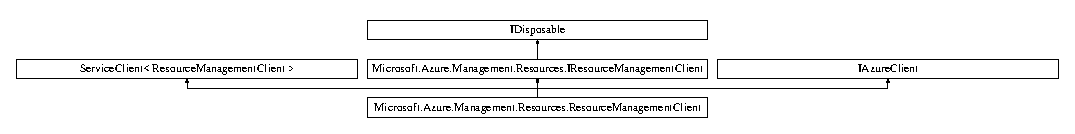
\includegraphics[height=1.346154cm]{class_microsoft_1_1_azure_1_1_management_1_1_resources_1_1_resource_management_client}
\end{center}
\end{figure}
\subsection*{Public Member Functions}
\begin{DoxyCompactItemize}
\item 
\hyperlink{class_microsoft_1_1_azure_1_1_management_1_1_resources_1_1_resource_management_client_a7c3b2493113102041854155b7cd29800}{Resource\+Management\+Client} (Service\+Client\+Credentials credentials, params Delegating\+Handler\mbox{[}$\,$\mbox{]} handlers)
\begin{DoxyCompactList}\small\item\em Initializes a new instance of the \hyperlink{class_microsoft_1_1_azure_1_1_management_1_1_resources_1_1_resource_management_client}{Resource\+Management\+Client} class. \end{DoxyCompactList}\item 
\hyperlink{class_microsoft_1_1_azure_1_1_management_1_1_resources_1_1_resource_management_client_aab315d4d0e5bb057d024a3fe2102a048}{Resource\+Management\+Client} (Service\+Client\+Credentials credentials, Http\+Client\+Handler root\+Handler, params Delegating\+Handler\mbox{[}$\,$\mbox{]} handlers)
\begin{DoxyCompactList}\small\item\em Initializes a new instance of the \hyperlink{class_microsoft_1_1_azure_1_1_management_1_1_resources_1_1_resource_management_client}{Resource\+Management\+Client} class. \end{DoxyCompactList}\item 
\hyperlink{class_microsoft_1_1_azure_1_1_management_1_1_resources_1_1_resource_management_client_a122cb72ec5d69862c51888f2a1e1eb44}{Resource\+Management\+Client} (Uri base\+Uri, Service\+Client\+Credentials credentials, params Delegating\+Handler\mbox{[}$\,$\mbox{]} handlers)
\begin{DoxyCompactList}\small\item\em Initializes a new instance of the \hyperlink{class_microsoft_1_1_azure_1_1_management_1_1_resources_1_1_resource_management_client}{Resource\+Management\+Client} class. \end{DoxyCompactList}\item 
\hyperlink{class_microsoft_1_1_azure_1_1_management_1_1_resources_1_1_resource_management_client_af0299a1bfe5aa8d89754dce429048576}{Resource\+Management\+Client} (Uri base\+Uri, Service\+Client\+Credentials credentials, Http\+Client\+Handler root\+Handler, params Delegating\+Handler\mbox{[}$\,$\mbox{]} handlers)
\begin{DoxyCompactList}\small\item\em Initializes a new instance of the \hyperlink{class_microsoft_1_1_azure_1_1_management_1_1_resources_1_1_resource_management_client}{Resource\+Management\+Client} class. \end{DoxyCompactList}\end{DoxyCompactItemize}
\subsection*{Protected Member Functions}
\begin{DoxyCompactItemize}
\item 
\hyperlink{class_microsoft_1_1_azure_1_1_management_1_1_resources_1_1_resource_management_client_a25717e3e6f08ff66622ecfdecaecd73f}{Resource\+Management\+Client} (params Delegating\+Handler\mbox{[}$\,$\mbox{]} handlers)
\begin{DoxyCompactList}\small\item\em Initializes a new instance of the \hyperlink{class_microsoft_1_1_azure_1_1_management_1_1_resources_1_1_resource_management_client}{Resource\+Management\+Client} class. \end{DoxyCompactList}\item 
\hyperlink{class_microsoft_1_1_azure_1_1_management_1_1_resources_1_1_resource_management_client_a29fd45246a89948d61e5ec6db8c7730b}{Resource\+Management\+Client} (Http\+Client\+Handler root\+Handler, params Delegating\+Handler\mbox{[}$\,$\mbox{]} handlers)
\begin{DoxyCompactList}\small\item\em Initializes a new instance of the \hyperlink{class_microsoft_1_1_azure_1_1_management_1_1_resources_1_1_resource_management_client}{Resource\+Management\+Client} class. \end{DoxyCompactList}\item 
\hyperlink{class_microsoft_1_1_azure_1_1_management_1_1_resources_1_1_resource_management_client_a5a5d2d72d9cd93efeac6042f182635ad}{Resource\+Management\+Client} (Uri base\+Uri, params Delegating\+Handler\mbox{[}$\,$\mbox{]} handlers)
\begin{DoxyCompactList}\small\item\em Initializes a new instance of the \hyperlink{class_microsoft_1_1_azure_1_1_management_1_1_resources_1_1_resource_management_client}{Resource\+Management\+Client} class. \end{DoxyCompactList}\item 
\hyperlink{class_microsoft_1_1_azure_1_1_management_1_1_resources_1_1_resource_management_client_a019102f4f8be6c98a0d3fd63f4d14270}{Resource\+Management\+Client} (Uri base\+Uri, Http\+Client\+Handler root\+Handler, params Delegating\+Handler\mbox{[}$\,$\mbox{]} handlers)
\begin{DoxyCompactList}\small\item\em Initializes a new instance of the \hyperlink{class_microsoft_1_1_azure_1_1_management_1_1_resources_1_1_resource_management_client}{Resource\+Management\+Client} class. \end{DoxyCompactList}\end{DoxyCompactItemize}
\subsection*{Properties}
\begin{DoxyCompactItemize}
\item 
Uri \hyperlink{class_microsoft_1_1_azure_1_1_management_1_1_resources_1_1_resource_management_client_a12157fa76c86043c0bbbc1bfbaf9f943}{Base\+Uri}\hspace{0.3cm}{\ttfamily  \mbox{[}get, set\mbox{]}}
\begin{DoxyCompactList}\small\item\em The base U\+RI of the service. \end{DoxyCompactList}\item 
Json\+Serializer\+Settings \hyperlink{class_microsoft_1_1_azure_1_1_management_1_1_resources_1_1_resource_management_client_a5c9bf84ada5a76a9a0ff7f4d7ec05c96}{Serialization\+Settings}\hspace{0.3cm}{\ttfamily  \mbox{[}get\mbox{]}}
\begin{DoxyCompactList}\small\item\em Gets or sets json serialization settings. \end{DoxyCompactList}\item 
Json\+Serializer\+Settings \hyperlink{class_microsoft_1_1_azure_1_1_management_1_1_resources_1_1_resource_management_client_a68ccbfd8a78c31c86299f8dca01f7eb1}{Deserialization\+Settings}\hspace{0.3cm}{\ttfamily  \mbox{[}get\mbox{]}}
\begin{DoxyCompactList}\small\item\em Gets or sets json deserialization settings. \end{DoxyCompactList}\item 
Service\+Client\+Credentials \hyperlink{class_microsoft_1_1_azure_1_1_management_1_1_resources_1_1_resource_management_client_a0a584166be337b158c3bd54845e5d124}{Credentials}\hspace{0.3cm}{\ttfamily  \mbox{[}get\mbox{]}}
\begin{DoxyCompactList}\small\item\em The management credentials for \hyperlink{namespace_microsoft_1_1_azure}{Azure}. \end{DoxyCompactList}\item 
string \hyperlink{class_microsoft_1_1_azure_1_1_management_1_1_resources_1_1_resource_management_client_a802627c8b37d0a015887bb3d6e1beb32}{Subscription\+Id}\hspace{0.3cm}{\ttfamily  \mbox{[}get, set\mbox{]}}
\begin{DoxyCompactList}\small\item\em Gets subscription credentials which uniquely identify \hyperlink{namespace_microsoft}{Microsoft} \hyperlink{namespace_microsoft_1_1_azure}{Azure} subscription. The subscription ID forms part of the U\+RI for every service call. \end{DoxyCompactList}\item 
string \hyperlink{class_microsoft_1_1_azure_1_1_management_1_1_resources_1_1_resource_management_client_aea51a4e00dde5b781e6f692e1ae2bc46}{Api\+Version}\hspace{0.3cm}{\ttfamily  \mbox{[}get\mbox{]}}
\begin{DoxyCompactList}\small\item\em Client Api Version. \end{DoxyCompactList}\item 
string \hyperlink{class_microsoft_1_1_azure_1_1_management_1_1_resources_1_1_resource_management_client_af3643c8e63b7c9f85c7c323f216f08c9}{Accept\+Language}\hspace{0.3cm}{\ttfamily  \mbox{[}get, set\mbox{]}}
\begin{DoxyCompactList}\small\item\em Gets or sets the preferred language for the response. \end{DoxyCompactList}\item 
int \hyperlink{class_microsoft_1_1_azure_1_1_management_1_1_resources_1_1_resource_management_client_ad3b245357fb89a925bcec2c0cc6fe300}{Long\+Running\+Operation\+Retry\+Timeout}\hspace{0.3cm}{\ttfamily  \mbox{[}get, set\mbox{]}}
\begin{DoxyCompactList}\small\item\em The retry timeout for Long Running Operations. \end{DoxyCompactList}\item 
virtual \hyperlink{interface_microsoft_1_1_azure_1_1_management_1_1_resources_1_1_i_deployments_operations}{I\+Deployments\+Operations} {\bfseries Deployments}\hspace{0.3cm}{\ttfamily  \mbox{[}get\mbox{]}}\hypertarget{class_microsoft_1_1_azure_1_1_management_1_1_resources_1_1_resource_management_client_aaba91c1c3605e83d38a6a6f03f15c5e4}{}\label{class_microsoft_1_1_azure_1_1_management_1_1_resources_1_1_resource_management_client_aaba91c1c3605e83d38a6a6f03f15c5e4}

\item 
virtual \hyperlink{interface_microsoft_1_1_azure_1_1_management_1_1_resources_1_1_i_providers_operations}{I\+Providers\+Operations} {\bfseries Providers}\hspace{0.3cm}{\ttfamily  \mbox{[}get\mbox{]}}\hypertarget{class_microsoft_1_1_azure_1_1_management_1_1_resources_1_1_resource_management_client_a0db61f31aa1e02dd057e99bb75c4ffe2}{}\label{class_microsoft_1_1_azure_1_1_management_1_1_resources_1_1_resource_management_client_a0db61f31aa1e02dd057e99bb75c4ffe2}

\item 
virtual \hyperlink{interface_microsoft_1_1_azure_1_1_management_1_1_resources_1_1_i_resource_groups_operations}{I\+Resource\+Groups\+Operations} {\bfseries Resource\+Groups}\hspace{0.3cm}{\ttfamily  \mbox{[}get\mbox{]}}\hypertarget{class_microsoft_1_1_azure_1_1_management_1_1_resources_1_1_resource_management_client_aeef4d7191da64b6b60c77127634b6afd}{}\label{class_microsoft_1_1_azure_1_1_management_1_1_resources_1_1_resource_management_client_aeef4d7191da64b6b60c77127634b6afd}

\item 
virtual \hyperlink{interface_microsoft_1_1_azure_1_1_management_1_1_resources_1_1_i_resources_operations}{I\+Resources\+Operations} {\bfseries Resources}\hspace{0.3cm}{\ttfamily  \mbox{[}get\mbox{]}}\hypertarget{class_microsoft_1_1_azure_1_1_management_1_1_resources_1_1_resource_management_client_a53f1a91a2837cb2b233860cf7de443a1}{}\label{class_microsoft_1_1_azure_1_1_management_1_1_resources_1_1_resource_management_client_a53f1a91a2837cb2b233860cf7de443a1}

\item 
virtual \hyperlink{interface_microsoft_1_1_azure_1_1_management_1_1_resources_1_1_i_tags_operations}{I\+Tags\+Operations} {\bfseries Tags}\hspace{0.3cm}{\ttfamily  \mbox{[}get\mbox{]}}\hypertarget{class_microsoft_1_1_azure_1_1_management_1_1_resources_1_1_resource_management_client_aa074aa01df434a06329ded53732dc7fa}{}\label{class_microsoft_1_1_azure_1_1_management_1_1_resources_1_1_resource_management_client_aa074aa01df434a06329ded53732dc7fa}

\item 
virtual \hyperlink{interface_microsoft_1_1_azure_1_1_management_1_1_resources_1_1_i_deployment_operations_operations}{I\+Deployment\+Operations\+Operations} {\bfseries Deployment\+Operations}\hspace{0.3cm}{\ttfamily  \mbox{[}get\mbox{]}}\hypertarget{class_microsoft_1_1_azure_1_1_management_1_1_resources_1_1_resource_management_client_a7382a07d0e55f6a2f2dbefdf11a26caa}{}\label{class_microsoft_1_1_azure_1_1_management_1_1_resources_1_1_resource_management_client_a7382a07d0e55f6a2f2dbefdf11a26caa}

\item 
virtual \hyperlink{interface_microsoft_1_1_azure_1_1_management_1_1_resources_1_1_i_resource_provider_operation_details_operations}{I\+Resource\+Provider\+Operation\+Details\+Operations} {\bfseries Resource\+Provider\+Operation\+Details}\hspace{0.3cm}{\ttfamily  \mbox{[}get\mbox{]}}\hypertarget{class_microsoft_1_1_azure_1_1_management_1_1_resources_1_1_resource_management_client_a19e80e212d6ebe4088513ae1984d88aa}{}\label{class_microsoft_1_1_azure_1_1_management_1_1_resources_1_1_resource_management_client_a19e80e212d6ebe4088513ae1984d88aa}

\item 
virtual \hyperlink{interface_microsoft_1_1_azure_1_1_management_1_1_resources_1_1_i_policy_definitions_operations}{I\+Policy\+Definitions\+Operations} {\bfseries Policy\+Definitions}\hspace{0.3cm}{\ttfamily  \mbox{[}get\mbox{]}}\hypertarget{class_microsoft_1_1_azure_1_1_management_1_1_resources_1_1_resource_management_client_ae7c4f0cf2871a8be9db56234b852d822}{}\label{class_microsoft_1_1_azure_1_1_management_1_1_resources_1_1_resource_management_client_ae7c4f0cf2871a8be9db56234b852d822}

\item 
virtual \hyperlink{interface_microsoft_1_1_azure_1_1_management_1_1_resources_1_1_i_policy_assignments_operations}{I\+Policy\+Assignments\+Operations} {\bfseries Policy\+Assignments}\hspace{0.3cm}{\ttfamily  \mbox{[}get\mbox{]}}\hypertarget{class_microsoft_1_1_azure_1_1_management_1_1_resources_1_1_resource_management_client_abda1cfa14394fbf79f41b054a4e57766}{}\label{class_microsoft_1_1_azure_1_1_management_1_1_resources_1_1_resource_management_client_abda1cfa14394fbf79f41b054a4e57766}

\end{DoxyCompactItemize}


\subsection{Detailed Description}




\subsection{Constructor \& Destructor Documentation}
\index{Microsoft\+::\+Azure\+::\+Management\+::\+Resources\+::\+Resource\+Management\+Client@{Microsoft\+::\+Azure\+::\+Management\+::\+Resources\+::\+Resource\+Management\+Client}!Resource\+Management\+Client@{Resource\+Management\+Client}}
\index{Resource\+Management\+Client@{Resource\+Management\+Client}!Microsoft\+::\+Azure\+::\+Management\+::\+Resources\+::\+Resource\+Management\+Client@{Microsoft\+::\+Azure\+::\+Management\+::\+Resources\+::\+Resource\+Management\+Client}}
\subsubsection[{\texorpdfstring{Resource\+Management\+Client(params Delegating\+Handler[] handlers)}{ResourceManagementClient(params DelegatingHandler[] handlers)}}]{\setlength{\rightskip}{0pt plus 5cm}Microsoft.\+Azure.\+Management.\+Resources.\+Resource\+Management\+Client.\+Resource\+Management\+Client (
\begin{DoxyParamCaption}
\item[{params Delegating\+Handler\mbox{[}$\,$\mbox{]}}]{handlers}
\end{DoxyParamCaption}
)\hspace{0.3cm}{\ttfamily [inline]}, {\ttfamily [protected]}}\hypertarget{class_microsoft_1_1_azure_1_1_management_1_1_resources_1_1_resource_management_client_a25717e3e6f08ff66622ecfdecaecd73f}{}\label{class_microsoft_1_1_azure_1_1_management_1_1_resources_1_1_resource_management_client_a25717e3e6f08ff66622ecfdecaecd73f}


Initializes a new instance of the \hyperlink{class_microsoft_1_1_azure_1_1_management_1_1_resources_1_1_resource_management_client}{Resource\+Management\+Client} class. 


\begin{DoxyParams}{Parameters}
{\em handlers} & Optional. The delegating handlers to add to the http client pipeline. \\
\hline
\end{DoxyParams}
\index{Microsoft\+::\+Azure\+::\+Management\+::\+Resources\+::\+Resource\+Management\+Client@{Microsoft\+::\+Azure\+::\+Management\+::\+Resources\+::\+Resource\+Management\+Client}!Resource\+Management\+Client@{Resource\+Management\+Client}}
\index{Resource\+Management\+Client@{Resource\+Management\+Client}!Microsoft\+::\+Azure\+::\+Management\+::\+Resources\+::\+Resource\+Management\+Client@{Microsoft\+::\+Azure\+::\+Management\+::\+Resources\+::\+Resource\+Management\+Client}}
\subsubsection[{\texorpdfstring{Resource\+Management\+Client(\+Http\+Client\+Handler root\+Handler, params Delegating\+Handler[] handlers)}{ResourceManagementClient(HttpClientHandler rootHandler, params DelegatingHandler[] handlers)}}]{\setlength{\rightskip}{0pt plus 5cm}Microsoft.\+Azure.\+Management.\+Resources.\+Resource\+Management\+Client.\+Resource\+Management\+Client (
\begin{DoxyParamCaption}
\item[{Http\+Client\+Handler}]{root\+Handler, }
\item[{params Delegating\+Handler\mbox{[}$\,$\mbox{]}}]{handlers}
\end{DoxyParamCaption}
)\hspace{0.3cm}{\ttfamily [inline]}, {\ttfamily [protected]}}\hypertarget{class_microsoft_1_1_azure_1_1_management_1_1_resources_1_1_resource_management_client_a29fd45246a89948d61e5ec6db8c7730b}{}\label{class_microsoft_1_1_azure_1_1_management_1_1_resources_1_1_resource_management_client_a29fd45246a89948d61e5ec6db8c7730b}


Initializes a new instance of the \hyperlink{class_microsoft_1_1_azure_1_1_management_1_1_resources_1_1_resource_management_client}{Resource\+Management\+Client} class. 


\begin{DoxyParams}{Parameters}
{\em root\+Handler} & Optional. The http client handler used to handle http transport. \\
\hline
{\em handlers} & Optional. The delegating handlers to add to the http client pipeline. \\
\hline
\end{DoxyParams}
\index{Microsoft\+::\+Azure\+::\+Management\+::\+Resources\+::\+Resource\+Management\+Client@{Microsoft\+::\+Azure\+::\+Management\+::\+Resources\+::\+Resource\+Management\+Client}!Resource\+Management\+Client@{Resource\+Management\+Client}}
\index{Resource\+Management\+Client@{Resource\+Management\+Client}!Microsoft\+::\+Azure\+::\+Management\+::\+Resources\+::\+Resource\+Management\+Client@{Microsoft\+::\+Azure\+::\+Management\+::\+Resources\+::\+Resource\+Management\+Client}}
\subsubsection[{\texorpdfstring{Resource\+Management\+Client(\+Uri base\+Uri, params Delegating\+Handler[] handlers)}{ResourceManagementClient(Uri baseUri, params DelegatingHandler[] handlers)}}]{\setlength{\rightskip}{0pt plus 5cm}Microsoft.\+Azure.\+Management.\+Resources.\+Resource\+Management\+Client.\+Resource\+Management\+Client (
\begin{DoxyParamCaption}
\item[{Uri}]{base\+Uri, }
\item[{params Delegating\+Handler\mbox{[}$\,$\mbox{]}}]{handlers}
\end{DoxyParamCaption}
)\hspace{0.3cm}{\ttfamily [inline]}, {\ttfamily [protected]}}\hypertarget{class_microsoft_1_1_azure_1_1_management_1_1_resources_1_1_resource_management_client_a5a5d2d72d9cd93efeac6042f182635ad}{}\label{class_microsoft_1_1_azure_1_1_management_1_1_resources_1_1_resource_management_client_a5a5d2d72d9cd93efeac6042f182635ad}


Initializes a new instance of the \hyperlink{class_microsoft_1_1_azure_1_1_management_1_1_resources_1_1_resource_management_client}{Resource\+Management\+Client} class. 


\begin{DoxyParams}{Parameters}
{\em base\+Uri} & Optional. The base U\+RI of the service. \\
\hline
{\em handlers} & Optional. The delegating handlers to add to the http client pipeline. \\
\hline
\end{DoxyParams}
\index{Microsoft\+::\+Azure\+::\+Management\+::\+Resources\+::\+Resource\+Management\+Client@{Microsoft\+::\+Azure\+::\+Management\+::\+Resources\+::\+Resource\+Management\+Client}!Resource\+Management\+Client@{Resource\+Management\+Client}}
\index{Resource\+Management\+Client@{Resource\+Management\+Client}!Microsoft\+::\+Azure\+::\+Management\+::\+Resources\+::\+Resource\+Management\+Client@{Microsoft\+::\+Azure\+::\+Management\+::\+Resources\+::\+Resource\+Management\+Client}}
\subsubsection[{\texorpdfstring{Resource\+Management\+Client(\+Uri base\+Uri, Http\+Client\+Handler root\+Handler, params Delegating\+Handler[] handlers)}{ResourceManagementClient(Uri baseUri, HttpClientHandler rootHandler, params DelegatingHandler[] handlers)}}]{\setlength{\rightskip}{0pt plus 5cm}Microsoft.\+Azure.\+Management.\+Resources.\+Resource\+Management\+Client.\+Resource\+Management\+Client (
\begin{DoxyParamCaption}
\item[{Uri}]{base\+Uri, }
\item[{Http\+Client\+Handler}]{root\+Handler, }
\item[{params Delegating\+Handler\mbox{[}$\,$\mbox{]}}]{handlers}
\end{DoxyParamCaption}
)\hspace{0.3cm}{\ttfamily [inline]}, {\ttfamily [protected]}}\hypertarget{class_microsoft_1_1_azure_1_1_management_1_1_resources_1_1_resource_management_client_a019102f4f8be6c98a0d3fd63f4d14270}{}\label{class_microsoft_1_1_azure_1_1_management_1_1_resources_1_1_resource_management_client_a019102f4f8be6c98a0d3fd63f4d14270}


Initializes a new instance of the \hyperlink{class_microsoft_1_1_azure_1_1_management_1_1_resources_1_1_resource_management_client}{Resource\+Management\+Client} class. 


\begin{DoxyParams}{Parameters}
{\em base\+Uri} & Optional. The base U\+RI of the service. \\
\hline
{\em root\+Handler} & Optional. The http client handler used to handle http transport. \\
\hline
{\em handlers} & Optional. The delegating handlers to add to the http client pipeline. \\
\hline
\end{DoxyParams}
\index{Microsoft\+::\+Azure\+::\+Management\+::\+Resources\+::\+Resource\+Management\+Client@{Microsoft\+::\+Azure\+::\+Management\+::\+Resources\+::\+Resource\+Management\+Client}!Resource\+Management\+Client@{Resource\+Management\+Client}}
\index{Resource\+Management\+Client@{Resource\+Management\+Client}!Microsoft\+::\+Azure\+::\+Management\+::\+Resources\+::\+Resource\+Management\+Client@{Microsoft\+::\+Azure\+::\+Management\+::\+Resources\+::\+Resource\+Management\+Client}}
\subsubsection[{\texorpdfstring{Resource\+Management\+Client(\+Service\+Client\+Credentials credentials, params Delegating\+Handler[] handlers)}{ResourceManagementClient(ServiceClientCredentials credentials, params DelegatingHandler[] handlers)}}]{\setlength{\rightskip}{0pt plus 5cm}Microsoft.\+Azure.\+Management.\+Resources.\+Resource\+Management\+Client.\+Resource\+Management\+Client (
\begin{DoxyParamCaption}
\item[{Service\+Client\+Credentials}]{credentials, }
\item[{params Delegating\+Handler\mbox{[}$\,$\mbox{]}}]{handlers}
\end{DoxyParamCaption}
)\hspace{0.3cm}{\ttfamily [inline]}}\hypertarget{class_microsoft_1_1_azure_1_1_management_1_1_resources_1_1_resource_management_client_a7c3b2493113102041854155b7cd29800}{}\label{class_microsoft_1_1_azure_1_1_management_1_1_resources_1_1_resource_management_client_a7c3b2493113102041854155b7cd29800}


Initializes a new instance of the \hyperlink{class_microsoft_1_1_azure_1_1_management_1_1_resources_1_1_resource_management_client}{Resource\+Management\+Client} class. 


\begin{DoxyParams}{Parameters}
{\em credentials} & Required. The management credentials for \hyperlink{namespace_microsoft_1_1_azure}{Azure}. \\
\hline
{\em handlers} & Optional. The delegating handlers to add to the http client pipeline. \\
\hline
\end{DoxyParams}
\index{Microsoft\+::\+Azure\+::\+Management\+::\+Resources\+::\+Resource\+Management\+Client@{Microsoft\+::\+Azure\+::\+Management\+::\+Resources\+::\+Resource\+Management\+Client}!Resource\+Management\+Client@{Resource\+Management\+Client}}
\index{Resource\+Management\+Client@{Resource\+Management\+Client}!Microsoft\+::\+Azure\+::\+Management\+::\+Resources\+::\+Resource\+Management\+Client@{Microsoft\+::\+Azure\+::\+Management\+::\+Resources\+::\+Resource\+Management\+Client}}
\subsubsection[{\texorpdfstring{Resource\+Management\+Client(\+Service\+Client\+Credentials credentials, Http\+Client\+Handler root\+Handler, params Delegating\+Handler[] handlers)}{ResourceManagementClient(ServiceClientCredentials credentials, HttpClientHandler rootHandler, params DelegatingHandler[] handlers)}}]{\setlength{\rightskip}{0pt plus 5cm}Microsoft.\+Azure.\+Management.\+Resources.\+Resource\+Management\+Client.\+Resource\+Management\+Client (
\begin{DoxyParamCaption}
\item[{Service\+Client\+Credentials}]{credentials, }
\item[{Http\+Client\+Handler}]{root\+Handler, }
\item[{params Delegating\+Handler\mbox{[}$\,$\mbox{]}}]{handlers}
\end{DoxyParamCaption}
)\hspace{0.3cm}{\ttfamily [inline]}}\hypertarget{class_microsoft_1_1_azure_1_1_management_1_1_resources_1_1_resource_management_client_aab315d4d0e5bb057d024a3fe2102a048}{}\label{class_microsoft_1_1_azure_1_1_management_1_1_resources_1_1_resource_management_client_aab315d4d0e5bb057d024a3fe2102a048}


Initializes a new instance of the \hyperlink{class_microsoft_1_1_azure_1_1_management_1_1_resources_1_1_resource_management_client}{Resource\+Management\+Client} class. 


\begin{DoxyParams}{Parameters}
{\em credentials} & Required. The management credentials for \hyperlink{namespace_microsoft_1_1_azure}{Azure}. \\
\hline
{\em root\+Handler} & Optional. The http client handler used to handle http transport. \\
\hline
{\em handlers} & Optional. The delegating handlers to add to the http client pipeline. \\
\hline
\end{DoxyParams}
\index{Microsoft\+::\+Azure\+::\+Management\+::\+Resources\+::\+Resource\+Management\+Client@{Microsoft\+::\+Azure\+::\+Management\+::\+Resources\+::\+Resource\+Management\+Client}!Resource\+Management\+Client@{Resource\+Management\+Client}}
\index{Resource\+Management\+Client@{Resource\+Management\+Client}!Microsoft\+::\+Azure\+::\+Management\+::\+Resources\+::\+Resource\+Management\+Client@{Microsoft\+::\+Azure\+::\+Management\+::\+Resources\+::\+Resource\+Management\+Client}}
\subsubsection[{\texorpdfstring{Resource\+Management\+Client(\+Uri base\+Uri, Service\+Client\+Credentials credentials, params Delegating\+Handler[] handlers)}{ResourceManagementClient(Uri baseUri, ServiceClientCredentials credentials, params DelegatingHandler[] handlers)}}]{\setlength{\rightskip}{0pt plus 5cm}Microsoft.\+Azure.\+Management.\+Resources.\+Resource\+Management\+Client.\+Resource\+Management\+Client (
\begin{DoxyParamCaption}
\item[{Uri}]{base\+Uri, }
\item[{Service\+Client\+Credentials}]{credentials, }
\item[{params Delegating\+Handler\mbox{[}$\,$\mbox{]}}]{handlers}
\end{DoxyParamCaption}
)\hspace{0.3cm}{\ttfamily [inline]}}\hypertarget{class_microsoft_1_1_azure_1_1_management_1_1_resources_1_1_resource_management_client_a122cb72ec5d69862c51888f2a1e1eb44}{}\label{class_microsoft_1_1_azure_1_1_management_1_1_resources_1_1_resource_management_client_a122cb72ec5d69862c51888f2a1e1eb44}


Initializes a new instance of the \hyperlink{class_microsoft_1_1_azure_1_1_management_1_1_resources_1_1_resource_management_client}{Resource\+Management\+Client} class. 


\begin{DoxyParams}{Parameters}
{\em base\+Uri} & Optional. The base U\+RI of the service. \\
\hline
{\em credentials} & Required. The management credentials for \hyperlink{namespace_microsoft_1_1_azure}{Azure}. \\
\hline
{\em handlers} & Optional. The delegating handlers to add to the http client pipeline. \\
\hline
\end{DoxyParams}
\index{Microsoft\+::\+Azure\+::\+Management\+::\+Resources\+::\+Resource\+Management\+Client@{Microsoft\+::\+Azure\+::\+Management\+::\+Resources\+::\+Resource\+Management\+Client}!Resource\+Management\+Client@{Resource\+Management\+Client}}
\index{Resource\+Management\+Client@{Resource\+Management\+Client}!Microsoft\+::\+Azure\+::\+Management\+::\+Resources\+::\+Resource\+Management\+Client@{Microsoft\+::\+Azure\+::\+Management\+::\+Resources\+::\+Resource\+Management\+Client}}
\subsubsection[{\texorpdfstring{Resource\+Management\+Client(\+Uri base\+Uri, Service\+Client\+Credentials credentials, Http\+Client\+Handler root\+Handler, params Delegating\+Handler[] handlers)}{ResourceManagementClient(Uri baseUri, ServiceClientCredentials credentials, HttpClientHandler rootHandler, params DelegatingHandler[] handlers)}}]{\setlength{\rightskip}{0pt plus 5cm}Microsoft.\+Azure.\+Management.\+Resources.\+Resource\+Management\+Client.\+Resource\+Management\+Client (
\begin{DoxyParamCaption}
\item[{Uri}]{base\+Uri, }
\item[{Service\+Client\+Credentials}]{credentials, }
\item[{Http\+Client\+Handler}]{root\+Handler, }
\item[{params Delegating\+Handler\mbox{[}$\,$\mbox{]}}]{handlers}
\end{DoxyParamCaption}
)\hspace{0.3cm}{\ttfamily [inline]}}\hypertarget{class_microsoft_1_1_azure_1_1_management_1_1_resources_1_1_resource_management_client_af0299a1bfe5aa8d89754dce429048576}{}\label{class_microsoft_1_1_azure_1_1_management_1_1_resources_1_1_resource_management_client_af0299a1bfe5aa8d89754dce429048576}


Initializes a new instance of the \hyperlink{class_microsoft_1_1_azure_1_1_management_1_1_resources_1_1_resource_management_client}{Resource\+Management\+Client} class. 


\begin{DoxyParams}{Parameters}
{\em base\+Uri} & Optional. The base U\+RI of the service. \\
\hline
{\em credentials} & Required. The management credentials for \hyperlink{namespace_microsoft_1_1_azure}{Azure}. \\
\hline
{\em root\+Handler} & Optional. The http client handler used to handle http transport. \\
\hline
{\em handlers} & Optional. The delegating handlers to add to the http client pipeline. \\
\hline
\end{DoxyParams}


\subsection{Property Documentation}
\index{Microsoft\+::\+Azure\+::\+Management\+::\+Resources\+::\+Resource\+Management\+Client@{Microsoft\+::\+Azure\+::\+Management\+::\+Resources\+::\+Resource\+Management\+Client}!Accept\+Language@{Accept\+Language}}
\index{Accept\+Language@{Accept\+Language}!Microsoft\+::\+Azure\+::\+Management\+::\+Resources\+::\+Resource\+Management\+Client@{Microsoft\+::\+Azure\+::\+Management\+::\+Resources\+::\+Resource\+Management\+Client}}
\subsubsection[{\texorpdfstring{Accept\+Language}{AcceptLanguage}}]{\setlength{\rightskip}{0pt plus 5cm}string Microsoft.\+Azure.\+Management.\+Resources.\+Resource\+Management\+Client.\+Accept\+Language\hspace{0.3cm}{\ttfamily [get]}, {\ttfamily [set]}}\hypertarget{class_microsoft_1_1_azure_1_1_management_1_1_resources_1_1_resource_management_client_af3643c8e63b7c9f85c7c323f216f08c9}{}\label{class_microsoft_1_1_azure_1_1_management_1_1_resources_1_1_resource_management_client_af3643c8e63b7c9f85c7c323f216f08c9}


Gets or sets the preferred language for the response. 

\index{Microsoft\+::\+Azure\+::\+Management\+::\+Resources\+::\+Resource\+Management\+Client@{Microsoft\+::\+Azure\+::\+Management\+::\+Resources\+::\+Resource\+Management\+Client}!Api\+Version@{Api\+Version}}
\index{Api\+Version@{Api\+Version}!Microsoft\+::\+Azure\+::\+Management\+::\+Resources\+::\+Resource\+Management\+Client@{Microsoft\+::\+Azure\+::\+Management\+::\+Resources\+::\+Resource\+Management\+Client}}
\subsubsection[{\texorpdfstring{Api\+Version}{ApiVersion}}]{\setlength{\rightskip}{0pt plus 5cm}string Microsoft.\+Azure.\+Management.\+Resources.\+Resource\+Management\+Client.\+Api\+Version\hspace{0.3cm}{\ttfamily [get]}}\hypertarget{class_microsoft_1_1_azure_1_1_management_1_1_resources_1_1_resource_management_client_aea51a4e00dde5b781e6f692e1ae2bc46}{}\label{class_microsoft_1_1_azure_1_1_management_1_1_resources_1_1_resource_management_client_aea51a4e00dde5b781e6f692e1ae2bc46}


Client Api Version. 

\index{Microsoft\+::\+Azure\+::\+Management\+::\+Resources\+::\+Resource\+Management\+Client@{Microsoft\+::\+Azure\+::\+Management\+::\+Resources\+::\+Resource\+Management\+Client}!Base\+Uri@{Base\+Uri}}
\index{Base\+Uri@{Base\+Uri}!Microsoft\+::\+Azure\+::\+Management\+::\+Resources\+::\+Resource\+Management\+Client@{Microsoft\+::\+Azure\+::\+Management\+::\+Resources\+::\+Resource\+Management\+Client}}
\subsubsection[{\texorpdfstring{Base\+Uri}{BaseUri}}]{\setlength{\rightskip}{0pt plus 5cm}Uri Microsoft.\+Azure.\+Management.\+Resources.\+Resource\+Management\+Client.\+Base\+Uri\hspace{0.3cm}{\ttfamily [get]}, {\ttfamily [set]}}\hypertarget{class_microsoft_1_1_azure_1_1_management_1_1_resources_1_1_resource_management_client_a12157fa76c86043c0bbbc1bfbaf9f943}{}\label{class_microsoft_1_1_azure_1_1_management_1_1_resources_1_1_resource_management_client_a12157fa76c86043c0bbbc1bfbaf9f943}


The base U\+RI of the service. 

\index{Microsoft\+::\+Azure\+::\+Management\+::\+Resources\+::\+Resource\+Management\+Client@{Microsoft\+::\+Azure\+::\+Management\+::\+Resources\+::\+Resource\+Management\+Client}!Credentials@{Credentials}}
\index{Credentials@{Credentials}!Microsoft\+::\+Azure\+::\+Management\+::\+Resources\+::\+Resource\+Management\+Client@{Microsoft\+::\+Azure\+::\+Management\+::\+Resources\+::\+Resource\+Management\+Client}}
\subsubsection[{\texorpdfstring{Credentials}{Credentials}}]{\setlength{\rightskip}{0pt plus 5cm}Service\+Client\+Credentials Microsoft.\+Azure.\+Management.\+Resources.\+Resource\+Management\+Client.\+Credentials\hspace{0.3cm}{\ttfamily [get]}}\hypertarget{class_microsoft_1_1_azure_1_1_management_1_1_resources_1_1_resource_management_client_a0a584166be337b158c3bd54845e5d124}{}\label{class_microsoft_1_1_azure_1_1_management_1_1_resources_1_1_resource_management_client_a0a584166be337b158c3bd54845e5d124}


The management credentials for \hyperlink{namespace_microsoft_1_1_azure}{Azure}. 

\index{Microsoft\+::\+Azure\+::\+Management\+::\+Resources\+::\+Resource\+Management\+Client@{Microsoft\+::\+Azure\+::\+Management\+::\+Resources\+::\+Resource\+Management\+Client}!Deserialization\+Settings@{Deserialization\+Settings}}
\index{Deserialization\+Settings@{Deserialization\+Settings}!Microsoft\+::\+Azure\+::\+Management\+::\+Resources\+::\+Resource\+Management\+Client@{Microsoft\+::\+Azure\+::\+Management\+::\+Resources\+::\+Resource\+Management\+Client}}
\subsubsection[{\texorpdfstring{Deserialization\+Settings}{DeserializationSettings}}]{\setlength{\rightskip}{0pt plus 5cm}Json\+Serializer\+Settings Microsoft.\+Azure.\+Management.\+Resources.\+Resource\+Management\+Client.\+Deserialization\+Settings\hspace{0.3cm}{\ttfamily [get]}}\hypertarget{class_microsoft_1_1_azure_1_1_management_1_1_resources_1_1_resource_management_client_a68ccbfd8a78c31c86299f8dca01f7eb1}{}\label{class_microsoft_1_1_azure_1_1_management_1_1_resources_1_1_resource_management_client_a68ccbfd8a78c31c86299f8dca01f7eb1}


Gets or sets json deserialization settings. 

\index{Microsoft\+::\+Azure\+::\+Management\+::\+Resources\+::\+Resource\+Management\+Client@{Microsoft\+::\+Azure\+::\+Management\+::\+Resources\+::\+Resource\+Management\+Client}!Long\+Running\+Operation\+Retry\+Timeout@{Long\+Running\+Operation\+Retry\+Timeout}}
\index{Long\+Running\+Operation\+Retry\+Timeout@{Long\+Running\+Operation\+Retry\+Timeout}!Microsoft\+::\+Azure\+::\+Management\+::\+Resources\+::\+Resource\+Management\+Client@{Microsoft\+::\+Azure\+::\+Management\+::\+Resources\+::\+Resource\+Management\+Client}}
\subsubsection[{\texorpdfstring{Long\+Running\+Operation\+Retry\+Timeout}{LongRunningOperationRetryTimeout}}]{\setlength{\rightskip}{0pt plus 5cm}int Microsoft.\+Azure.\+Management.\+Resources.\+Resource\+Management\+Client.\+Long\+Running\+Operation\+Retry\+Timeout\hspace{0.3cm}{\ttfamily [get]}, {\ttfamily [set]}}\hypertarget{class_microsoft_1_1_azure_1_1_management_1_1_resources_1_1_resource_management_client_ad3b245357fb89a925bcec2c0cc6fe300}{}\label{class_microsoft_1_1_azure_1_1_management_1_1_resources_1_1_resource_management_client_ad3b245357fb89a925bcec2c0cc6fe300}


The retry timeout for Long Running Operations. 

\index{Microsoft\+::\+Azure\+::\+Management\+::\+Resources\+::\+Resource\+Management\+Client@{Microsoft\+::\+Azure\+::\+Management\+::\+Resources\+::\+Resource\+Management\+Client}!Serialization\+Settings@{Serialization\+Settings}}
\index{Serialization\+Settings@{Serialization\+Settings}!Microsoft\+::\+Azure\+::\+Management\+::\+Resources\+::\+Resource\+Management\+Client@{Microsoft\+::\+Azure\+::\+Management\+::\+Resources\+::\+Resource\+Management\+Client}}
\subsubsection[{\texorpdfstring{Serialization\+Settings}{SerializationSettings}}]{\setlength{\rightskip}{0pt plus 5cm}Json\+Serializer\+Settings Microsoft.\+Azure.\+Management.\+Resources.\+Resource\+Management\+Client.\+Serialization\+Settings\hspace{0.3cm}{\ttfamily [get]}}\hypertarget{class_microsoft_1_1_azure_1_1_management_1_1_resources_1_1_resource_management_client_a5c9bf84ada5a76a9a0ff7f4d7ec05c96}{}\label{class_microsoft_1_1_azure_1_1_management_1_1_resources_1_1_resource_management_client_a5c9bf84ada5a76a9a0ff7f4d7ec05c96}


Gets or sets json serialization settings. 

\index{Microsoft\+::\+Azure\+::\+Management\+::\+Resources\+::\+Resource\+Management\+Client@{Microsoft\+::\+Azure\+::\+Management\+::\+Resources\+::\+Resource\+Management\+Client}!Subscription\+Id@{Subscription\+Id}}
\index{Subscription\+Id@{Subscription\+Id}!Microsoft\+::\+Azure\+::\+Management\+::\+Resources\+::\+Resource\+Management\+Client@{Microsoft\+::\+Azure\+::\+Management\+::\+Resources\+::\+Resource\+Management\+Client}}
\subsubsection[{\texorpdfstring{Subscription\+Id}{SubscriptionId}}]{\setlength{\rightskip}{0pt plus 5cm}string Microsoft.\+Azure.\+Management.\+Resources.\+Resource\+Management\+Client.\+Subscription\+Id\hspace{0.3cm}{\ttfamily [get]}, {\ttfamily [set]}}\hypertarget{class_microsoft_1_1_azure_1_1_management_1_1_resources_1_1_resource_management_client_a802627c8b37d0a015887bb3d6e1beb32}{}\label{class_microsoft_1_1_azure_1_1_management_1_1_resources_1_1_resource_management_client_a802627c8b37d0a015887bb3d6e1beb32}


Gets subscription credentials which uniquely identify \hyperlink{namespace_microsoft}{Microsoft} \hyperlink{namespace_microsoft_1_1_azure}{Azure} subscription. The subscription ID forms part of the U\+RI for every service call. 



The documentation for this class was generated from the following file\+:\begin{DoxyCompactItemize}
\item 
files/Resource\+Management\+Client.\+cs\end{DoxyCompactItemize}

\hypertarget{class_microsoft_1_1_azure_1_1_management_1_1_resources_1_1_subscription_client}{}\section{Microsoft.\+Azure.\+Management.\+Resources.\+Subscription\+Client Class Reference}
\label{class_microsoft_1_1_azure_1_1_management_1_1_resources_1_1_subscription_client}\index{Microsoft.\+Azure.\+Management.\+Resources.\+Subscription\+Client@{Microsoft.\+Azure.\+Management.\+Resources.\+Subscription\+Client}}


 


Inheritance diagram for Microsoft.\+Azure.\+Management.\+Resources.\+Subscription\+Client\+:\begin{figure}[H]
\begin{center}
\leavevmode
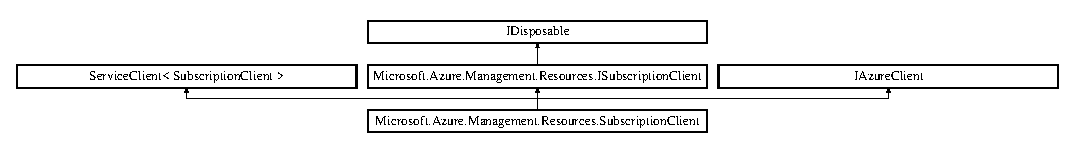
\includegraphics[height=1.555556cm]{class_microsoft_1_1_azure_1_1_management_1_1_resources_1_1_subscription_client}
\end{center}
\end{figure}
\subsection*{Public Member Functions}
\begin{DoxyCompactItemize}
\item 
\hyperlink{class_microsoft_1_1_azure_1_1_management_1_1_resources_1_1_subscription_client_a931c719e39cbf61ecc8f9fe0a286befb}{Subscription\+Client} (Service\+Client\+Credentials credentials, params Delegating\+Handler\mbox{[}$\,$\mbox{]} handlers)
\begin{DoxyCompactList}\small\item\em Initializes a new instance of the \hyperlink{class_microsoft_1_1_azure_1_1_management_1_1_resources_1_1_subscription_client}{Subscription\+Client} class. \end{DoxyCompactList}\item 
\hyperlink{class_microsoft_1_1_azure_1_1_management_1_1_resources_1_1_subscription_client_a45216f481936fc3f4a3929d627d31fef}{Subscription\+Client} (Service\+Client\+Credentials credentials, Http\+Client\+Handler root\+Handler, params Delegating\+Handler\mbox{[}$\,$\mbox{]} handlers)
\begin{DoxyCompactList}\small\item\em Initializes a new instance of the \hyperlink{class_microsoft_1_1_azure_1_1_management_1_1_resources_1_1_subscription_client}{Subscription\+Client} class. \end{DoxyCompactList}\item 
\hyperlink{class_microsoft_1_1_azure_1_1_management_1_1_resources_1_1_subscription_client_a1013e624adeaeb71c7b1736405192bc8}{Subscription\+Client} (Uri base\+Uri, Service\+Client\+Credentials credentials, params Delegating\+Handler\mbox{[}$\,$\mbox{]} handlers)
\begin{DoxyCompactList}\small\item\em Initializes a new instance of the \hyperlink{class_microsoft_1_1_azure_1_1_management_1_1_resources_1_1_subscription_client}{Subscription\+Client} class. \end{DoxyCompactList}\item 
\hyperlink{class_microsoft_1_1_azure_1_1_management_1_1_resources_1_1_subscription_client_afc24eb3b8408d05667b9d5e77f649d04}{Subscription\+Client} (Uri base\+Uri, Service\+Client\+Credentials credentials, Http\+Client\+Handler root\+Handler, params Delegating\+Handler\mbox{[}$\,$\mbox{]} handlers)
\begin{DoxyCompactList}\small\item\em Initializes a new instance of the \hyperlink{class_microsoft_1_1_azure_1_1_management_1_1_resources_1_1_subscription_client}{Subscription\+Client} class. \end{DoxyCompactList}\end{DoxyCompactItemize}
\subsection*{Protected Member Functions}
\begin{DoxyCompactItemize}
\item 
\hyperlink{class_microsoft_1_1_azure_1_1_management_1_1_resources_1_1_subscription_client_a08db5fed47828d80a3d14c530265db2a}{Subscription\+Client} (params Delegating\+Handler\mbox{[}$\,$\mbox{]} handlers)
\begin{DoxyCompactList}\small\item\em Initializes a new instance of the \hyperlink{class_microsoft_1_1_azure_1_1_management_1_1_resources_1_1_subscription_client}{Subscription\+Client} class. \end{DoxyCompactList}\item 
\hyperlink{class_microsoft_1_1_azure_1_1_management_1_1_resources_1_1_subscription_client_a227244485e4b902762e11d9921aaf202}{Subscription\+Client} (Http\+Client\+Handler root\+Handler, params Delegating\+Handler\mbox{[}$\,$\mbox{]} handlers)
\begin{DoxyCompactList}\small\item\em Initializes a new instance of the \hyperlink{class_microsoft_1_1_azure_1_1_management_1_1_resources_1_1_subscription_client}{Subscription\+Client} class. \end{DoxyCompactList}\item 
\hyperlink{class_microsoft_1_1_azure_1_1_management_1_1_resources_1_1_subscription_client_a119ddb7996450a8b61f805524fe5095a}{Subscription\+Client} (Uri base\+Uri, params Delegating\+Handler\mbox{[}$\,$\mbox{]} handlers)
\begin{DoxyCompactList}\small\item\em Initializes a new instance of the \hyperlink{class_microsoft_1_1_azure_1_1_management_1_1_resources_1_1_subscription_client}{Subscription\+Client} class. \end{DoxyCompactList}\item 
\hyperlink{class_microsoft_1_1_azure_1_1_management_1_1_resources_1_1_subscription_client_a5d89239dcbe8b75331c0844572a874f5}{Subscription\+Client} (Uri base\+Uri, Http\+Client\+Handler root\+Handler, params Delegating\+Handler\mbox{[}$\,$\mbox{]} handlers)
\begin{DoxyCompactList}\small\item\em Initializes a new instance of the \hyperlink{class_microsoft_1_1_azure_1_1_management_1_1_resources_1_1_subscription_client}{Subscription\+Client} class. \end{DoxyCompactList}\end{DoxyCompactItemize}
\subsection*{Properties}
\begin{DoxyCompactItemize}
\item 
Uri \hyperlink{class_microsoft_1_1_azure_1_1_management_1_1_resources_1_1_subscription_client_ab5876848c2253cbe2f84f98b4e7571e2}{Base\+Uri}\hspace{0.3cm}{\ttfamily  \mbox{[}get, set\mbox{]}}
\begin{DoxyCompactList}\small\item\em The base U\+RI of the service. \end{DoxyCompactList}\item 
Json\+Serializer\+Settings \hyperlink{class_microsoft_1_1_azure_1_1_management_1_1_resources_1_1_subscription_client_ae80cef67dabf656f811768833fa2d1fa}{Serialization\+Settings}\hspace{0.3cm}{\ttfamily  \mbox{[}get\mbox{]}}
\begin{DoxyCompactList}\small\item\em Gets or sets json serialization settings. \end{DoxyCompactList}\item 
Json\+Serializer\+Settings \hyperlink{class_microsoft_1_1_azure_1_1_management_1_1_resources_1_1_subscription_client_a8ef55e56f28601f1245f85acbcafc106}{Deserialization\+Settings}\hspace{0.3cm}{\ttfamily  \mbox{[}get\mbox{]}}
\begin{DoxyCompactList}\small\item\em Gets or sets json deserialization settings. \end{DoxyCompactList}\item 
Service\+Client\+Credentials \hyperlink{class_microsoft_1_1_azure_1_1_management_1_1_resources_1_1_subscription_client_a077fc135081e629980684d0d834ef70f}{Credentials}\hspace{0.3cm}{\ttfamily  \mbox{[}get\mbox{]}}
\begin{DoxyCompactList}\small\item\em The management credentials for \hyperlink{namespace_microsoft_1_1_azure}{Azure}. \end{DoxyCompactList}\item 
string \hyperlink{class_microsoft_1_1_azure_1_1_management_1_1_resources_1_1_subscription_client_a0f4b5173b00b37f6f78d31dd9a0ec352}{Subscription\+Id}\hspace{0.3cm}{\ttfamily  \mbox{[}get, set\mbox{]}}
\begin{DoxyCompactList}\small\item\em Gets subscription credentials which uniquely identify \hyperlink{namespace_microsoft}{Microsoft} \hyperlink{namespace_microsoft_1_1_azure}{Azure} subscription. The subscription ID forms part of the U\+RI for every service call. \end{DoxyCompactList}\item 
string \hyperlink{class_microsoft_1_1_azure_1_1_management_1_1_resources_1_1_subscription_client_abda07afb545fe259d63826a85960c528}{Api\+Version}\hspace{0.3cm}{\ttfamily  \mbox{[}get\mbox{]}}
\begin{DoxyCompactList}\small\item\em Client Api Version. \end{DoxyCompactList}\item 
string \hyperlink{class_microsoft_1_1_azure_1_1_management_1_1_resources_1_1_subscription_client_a655dec3210244f2c473a2e3201c30189}{Accept\+Language}\hspace{0.3cm}{\ttfamily  \mbox{[}get, set\mbox{]}}
\begin{DoxyCompactList}\small\item\em Gets or sets the preferred language for the response. \end{DoxyCompactList}\item 
int \hyperlink{class_microsoft_1_1_azure_1_1_management_1_1_resources_1_1_subscription_client_a0307675c0c36b17fc4ac0e1b2295c3e4}{Long\+Running\+Operation\+Retry\+Timeout}\hspace{0.3cm}{\ttfamily  \mbox{[}get, set\mbox{]}}
\begin{DoxyCompactList}\small\item\em The retry timeout for Long Running Operations. \end{DoxyCompactList}\item 
virtual \hyperlink{interface_microsoft_1_1_azure_1_1_management_1_1_resources_1_1_i_subscriptions_operations}{I\+Subscriptions\+Operations} {\bfseries Subscriptions}\hspace{0.3cm}{\ttfamily  \mbox{[}get\mbox{]}}\hypertarget{class_microsoft_1_1_azure_1_1_management_1_1_resources_1_1_subscription_client_aaaed37d21a575eaf68844f48f693f3bc}{}\label{class_microsoft_1_1_azure_1_1_management_1_1_resources_1_1_subscription_client_aaaed37d21a575eaf68844f48f693f3bc}

\item 
virtual \hyperlink{interface_microsoft_1_1_azure_1_1_management_1_1_resources_1_1_i_tenants_operations}{I\+Tenants\+Operations} {\bfseries Tenants}\hspace{0.3cm}{\ttfamily  \mbox{[}get\mbox{]}}\hypertarget{class_microsoft_1_1_azure_1_1_management_1_1_resources_1_1_subscription_client_aedff4dfb9c12efb93cf9d1f460c55c52}{}\label{class_microsoft_1_1_azure_1_1_management_1_1_resources_1_1_subscription_client_aedff4dfb9c12efb93cf9d1f460c55c52}

\end{DoxyCompactItemize}


\subsection{Detailed Description}




\subsection{Constructor \& Destructor Documentation}
\index{Microsoft\+::\+Azure\+::\+Management\+::\+Resources\+::\+Subscription\+Client@{Microsoft\+::\+Azure\+::\+Management\+::\+Resources\+::\+Subscription\+Client}!Subscription\+Client@{Subscription\+Client}}
\index{Subscription\+Client@{Subscription\+Client}!Microsoft\+::\+Azure\+::\+Management\+::\+Resources\+::\+Subscription\+Client@{Microsoft\+::\+Azure\+::\+Management\+::\+Resources\+::\+Subscription\+Client}}
\subsubsection[{\texorpdfstring{Subscription\+Client(params Delegating\+Handler[] handlers)}{SubscriptionClient(params DelegatingHandler[] handlers)}}]{\setlength{\rightskip}{0pt plus 5cm}Microsoft.\+Azure.\+Management.\+Resources.\+Subscription\+Client.\+Subscription\+Client (
\begin{DoxyParamCaption}
\item[{params Delegating\+Handler\mbox{[}$\,$\mbox{]}}]{handlers}
\end{DoxyParamCaption}
)\hspace{0.3cm}{\ttfamily [inline]}, {\ttfamily [protected]}}\hypertarget{class_microsoft_1_1_azure_1_1_management_1_1_resources_1_1_subscription_client_a08db5fed47828d80a3d14c530265db2a}{}\label{class_microsoft_1_1_azure_1_1_management_1_1_resources_1_1_subscription_client_a08db5fed47828d80a3d14c530265db2a}


Initializes a new instance of the \hyperlink{class_microsoft_1_1_azure_1_1_management_1_1_resources_1_1_subscription_client}{Subscription\+Client} class. 


\begin{DoxyParams}{Parameters}
{\em handlers} & Optional. The delegating handlers to add to the http client pipeline. \\
\hline
\end{DoxyParams}
\index{Microsoft\+::\+Azure\+::\+Management\+::\+Resources\+::\+Subscription\+Client@{Microsoft\+::\+Azure\+::\+Management\+::\+Resources\+::\+Subscription\+Client}!Subscription\+Client@{Subscription\+Client}}
\index{Subscription\+Client@{Subscription\+Client}!Microsoft\+::\+Azure\+::\+Management\+::\+Resources\+::\+Subscription\+Client@{Microsoft\+::\+Azure\+::\+Management\+::\+Resources\+::\+Subscription\+Client}}
\subsubsection[{\texorpdfstring{Subscription\+Client(\+Http\+Client\+Handler root\+Handler, params Delegating\+Handler[] handlers)}{SubscriptionClient(HttpClientHandler rootHandler, params DelegatingHandler[] handlers)}}]{\setlength{\rightskip}{0pt plus 5cm}Microsoft.\+Azure.\+Management.\+Resources.\+Subscription\+Client.\+Subscription\+Client (
\begin{DoxyParamCaption}
\item[{Http\+Client\+Handler}]{root\+Handler, }
\item[{params Delegating\+Handler\mbox{[}$\,$\mbox{]}}]{handlers}
\end{DoxyParamCaption}
)\hspace{0.3cm}{\ttfamily [inline]}, {\ttfamily [protected]}}\hypertarget{class_microsoft_1_1_azure_1_1_management_1_1_resources_1_1_subscription_client_a227244485e4b902762e11d9921aaf202}{}\label{class_microsoft_1_1_azure_1_1_management_1_1_resources_1_1_subscription_client_a227244485e4b902762e11d9921aaf202}


Initializes a new instance of the \hyperlink{class_microsoft_1_1_azure_1_1_management_1_1_resources_1_1_subscription_client}{Subscription\+Client} class. 


\begin{DoxyParams}{Parameters}
{\em root\+Handler} & Optional. The http client handler used to handle http transport. \\
\hline
{\em handlers} & Optional. The delegating handlers to add to the http client pipeline. \\
\hline
\end{DoxyParams}
\index{Microsoft\+::\+Azure\+::\+Management\+::\+Resources\+::\+Subscription\+Client@{Microsoft\+::\+Azure\+::\+Management\+::\+Resources\+::\+Subscription\+Client}!Subscription\+Client@{Subscription\+Client}}
\index{Subscription\+Client@{Subscription\+Client}!Microsoft\+::\+Azure\+::\+Management\+::\+Resources\+::\+Subscription\+Client@{Microsoft\+::\+Azure\+::\+Management\+::\+Resources\+::\+Subscription\+Client}}
\subsubsection[{\texorpdfstring{Subscription\+Client(\+Uri base\+Uri, params Delegating\+Handler[] handlers)}{SubscriptionClient(Uri baseUri, params DelegatingHandler[] handlers)}}]{\setlength{\rightskip}{0pt plus 5cm}Microsoft.\+Azure.\+Management.\+Resources.\+Subscription\+Client.\+Subscription\+Client (
\begin{DoxyParamCaption}
\item[{Uri}]{base\+Uri, }
\item[{params Delegating\+Handler\mbox{[}$\,$\mbox{]}}]{handlers}
\end{DoxyParamCaption}
)\hspace{0.3cm}{\ttfamily [inline]}, {\ttfamily [protected]}}\hypertarget{class_microsoft_1_1_azure_1_1_management_1_1_resources_1_1_subscription_client_a119ddb7996450a8b61f805524fe5095a}{}\label{class_microsoft_1_1_azure_1_1_management_1_1_resources_1_1_subscription_client_a119ddb7996450a8b61f805524fe5095a}


Initializes a new instance of the \hyperlink{class_microsoft_1_1_azure_1_1_management_1_1_resources_1_1_subscription_client}{Subscription\+Client} class. 


\begin{DoxyParams}{Parameters}
{\em base\+Uri} & Optional. The base U\+RI of the service. \\
\hline
{\em handlers} & Optional. The delegating handlers to add to the http client pipeline. \\
\hline
\end{DoxyParams}
\index{Microsoft\+::\+Azure\+::\+Management\+::\+Resources\+::\+Subscription\+Client@{Microsoft\+::\+Azure\+::\+Management\+::\+Resources\+::\+Subscription\+Client}!Subscription\+Client@{Subscription\+Client}}
\index{Subscription\+Client@{Subscription\+Client}!Microsoft\+::\+Azure\+::\+Management\+::\+Resources\+::\+Subscription\+Client@{Microsoft\+::\+Azure\+::\+Management\+::\+Resources\+::\+Subscription\+Client}}
\subsubsection[{\texorpdfstring{Subscription\+Client(\+Uri base\+Uri, Http\+Client\+Handler root\+Handler, params Delegating\+Handler[] handlers)}{SubscriptionClient(Uri baseUri, HttpClientHandler rootHandler, params DelegatingHandler[] handlers)}}]{\setlength{\rightskip}{0pt plus 5cm}Microsoft.\+Azure.\+Management.\+Resources.\+Subscription\+Client.\+Subscription\+Client (
\begin{DoxyParamCaption}
\item[{Uri}]{base\+Uri, }
\item[{Http\+Client\+Handler}]{root\+Handler, }
\item[{params Delegating\+Handler\mbox{[}$\,$\mbox{]}}]{handlers}
\end{DoxyParamCaption}
)\hspace{0.3cm}{\ttfamily [inline]}, {\ttfamily [protected]}}\hypertarget{class_microsoft_1_1_azure_1_1_management_1_1_resources_1_1_subscription_client_a5d89239dcbe8b75331c0844572a874f5}{}\label{class_microsoft_1_1_azure_1_1_management_1_1_resources_1_1_subscription_client_a5d89239dcbe8b75331c0844572a874f5}


Initializes a new instance of the \hyperlink{class_microsoft_1_1_azure_1_1_management_1_1_resources_1_1_subscription_client}{Subscription\+Client} class. 


\begin{DoxyParams}{Parameters}
{\em base\+Uri} & Optional. The base U\+RI of the service. \\
\hline
{\em root\+Handler} & Optional. The http client handler used to handle http transport. \\
\hline
{\em handlers} & Optional. The delegating handlers to add to the http client pipeline. \\
\hline
\end{DoxyParams}
\index{Microsoft\+::\+Azure\+::\+Management\+::\+Resources\+::\+Subscription\+Client@{Microsoft\+::\+Azure\+::\+Management\+::\+Resources\+::\+Subscription\+Client}!Subscription\+Client@{Subscription\+Client}}
\index{Subscription\+Client@{Subscription\+Client}!Microsoft\+::\+Azure\+::\+Management\+::\+Resources\+::\+Subscription\+Client@{Microsoft\+::\+Azure\+::\+Management\+::\+Resources\+::\+Subscription\+Client}}
\subsubsection[{\texorpdfstring{Subscription\+Client(\+Service\+Client\+Credentials credentials, params Delegating\+Handler[] handlers)}{SubscriptionClient(ServiceClientCredentials credentials, params DelegatingHandler[] handlers)}}]{\setlength{\rightskip}{0pt plus 5cm}Microsoft.\+Azure.\+Management.\+Resources.\+Subscription\+Client.\+Subscription\+Client (
\begin{DoxyParamCaption}
\item[{Service\+Client\+Credentials}]{credentials, }
\item[{params Delegating\+Handler\mbox{[}$\,$\mbox{]}}]{handlers}
\end{DoxyParamCaption}
)\hspace{0.3cm}{\ttfamily [inline]}}\hypertarget{class_microsoft_1_1_azure_1_1_management_1_1_resources_1_1_subscription_client_a931c719e39cbf61ecc8f9fe0a286befb}{}\label{class_microsoft_1_1_azure_1_1_management_1_1_resources_1_1_subscription_client_a931c719e39cbf61ecc8f9fe0a286befb}


Initializes a new instance of the \hyperlink{class_microsoft_1_1_azure_1_1_management_1_1_resources_1_1_subscription_client}{Subscription\+Client} class. 


\begin{DoxyParams}{Parameters}
{\em credentials} & Required. The management credentials for \hyperlink{namespace_microsoft_1_1_azure}{Azure}. \\
\hline
{\em handlers} & Optional. The delegating handlers to add to the http client pipeline. \\
\hline
\end{DoxyParams}
\index{Microsoft\+::\+Azure\+::\+Management\+::\+Resources\+::\+Subscription\+Client@{Microsoft\+::\+Azure\+::\+Management\+::\+Resources\+::\+Subscription\+Client}!Subscription\+Client@{Subscription\+Client}}
\index{Subscription\+Client@{Subscription\+Client}!Microsoft\+::\+Azure\+::\+Management\+::\+Resources\+::\+Subscription\+Client@{Microsoft\+::\+Azure\+::\+Management\+::\+Resources\+::\+Subscription\+Client}}
\subsubsection[{\texorpdfstring{Subscription\+Client(\+Service\+Client\+Credentials credentials, Http\+Client\+Handler root\+Handler, params Delegating\+Handler[] handlers)}{SubscriptionClient(ServiceClientCredentials credentials, HttpClientHandler rootHandler, params DelegatingHandler[] handlers)}}]{\setlength{\rightskip}{0pt plus 5cm}Microsoft.\+Azure.\+Management.\+Resources.\+Subscription\+Client.\+Subscription\+Client (
\begin{DoxyParamCaption}
\item[{Service\+Client\+Credentials}]{credentials, }
\item[{Http\+Client\+Handler}]{root\+Handler, }
\item[{params Delegating\+Handler\mbox{[}$\,$\mbox{]}}]{handlers}
\end{DoxyParamCaption}
)\hspace{0.3cm}{\ttfamily [inline]}}\hypertarget{class_microsoft_1_1_azure_1_1_management_1_1_resources_1_1_subscription_client_a45216f481936fc3f4a3929d627d31fef}{}\label{class_microsoft_1_1_azure_1_1_management_1_1_resources_1_1_subscription_client_a45216f481936fc3f4a3929d627d31fef}


Initializes a new instance of the \hyperlink{class_microsoft_1_1_azure_1_1_management_1_1_resources_1_1_subscription_client}{Subscription\+Client} class. 


\begin{DoxyParams}{Parameters}
{\em credentials} & Required. The management credentials for \hyperlink{namespace_microsoft_1_1_azure}{Azure}. \\
\hline
{\em root\+Handler} & Optional. The http client handler used to handle http transport. \\
\hline
{\em handlers} & Optional. The delegating handlers to add to the http client pipeline. \\
\hline
\end{DoxyParams}
\index{Microsoft\+::\+Azure\+::\+Management\+::\+Resources\+::\+Subscription\+Client@{Microsoft\+::\+Azure\+::\+Management\+::\+Resources\+::\+Subscription\+Client}!Subscription\+Client@{Subscription\+Client}}
\index{Subscription\+Client@{Subscription\+Client}!Microsoft\+::\+Azure\+::\+Management\+::\+Resources\+::\+Subscription\+Client@{Microsoft\+::\+Azure\+::\+Management\+::\+Resources\+::\+Subscription\+Client}}
\subsubsection[{\texorpdfstring{Subscription\+Client(\+Uri base\+Uri, Service\+Client\+Credentials credentials, params Delegating\+Handler[] handlers)}{SubscriptionClient(Uri baseUri, ServiceClientCredentials credentials, params DelegatingHandler[] handlers)}}]{\setlength{\rightskip}{0pt plus 5cm}Microsoft.\+Azure.\+Management.\+Resources.\+Subscription\+Client.\+Subscription\+Client (
\begin{DoxyParamCaption}
\item[{Uri}]{base\+Uri, }
\item[{Service\+Client\+Credentials}]{credentials, }
\item[{params Delegating\+Handler\mbox{[}$\,$\mbox{]}}]{handlers}
\end{DoxyParamCaption}
)\hspace{0.3cm}{\ttfamily [inline]}}\hypertarget{class_microsoft_1_1_azure_1_1_management_1_1_resources_1_1_subscription_client_a1013e624adeaeb71c7b1736405192bc8}{}\label{class_microsoft_1_1_azure_1_1_management_1_1_resources_1_1_subscription_client_a1013e624adeaeb71c7b1736405192bc8}


Initializes a new instance of the \hyperlink{class_microsoft_1_1_azure_1_1_management_1_1_resources_1_1_subscription_client}{Subscription\+Client} class. 


\begin{DoxyParams}{Parameters}
{\em base\+Uri} & Optional. The base U\+RI of the service. \\
\hline
{\em credentials} & Required. The management credentials for \hyperlink{namespace_microsoft_1_1_azure}{Azure}. \\
\hline
{\em handlers} & Optional. The delegating handlers to add to the http client pipeline. \\
\hline
\end{DoxyParams}
\index{Microsoft\+::\+Azure\+::\+Management\+::\+Resources\+::\+Subscription\+Client@{Microsoft\+::\+Azure\+::\+Management\+::\+Resources\+::\+Subscription\+Client}!Subscription\+Client@{Subscription\+Client}}
\index{Subscription\+Client@{Subscription\+Client}!Microsoft\+::\+Azure\+::\+Management\+::\+Resources\+::\+Subscription\+Client@{Microsoft\+::\+Azure\+::\+Management\+::\+Resources\+::\+Subscription\+Client}}
\subsubsection[{\texorpdfstring{Subscription\+Client(\+Uri base\+Uri, Service\+Client\+Credentials credentials, Http\+Client\+Handler root\+Handler, params Delegating\+Handler[] handlers)}{SubscriptionClient(Uri baseUri, ServiceClientCredentials credentials, HttpClientHandler rootHandler, params DelegatingHandler[] handlers)}}]{\setlength{\rightskip}{0pt plus 5cm}Microsoft.\+Azure.\+Management.\+Resources.\+Subscription\+Client.\+Subscription\+Client (
\begin{DoxyParamCaption}
\item[{Uri}]{base\+Uri, }
\item[{Service\+Client\+Credentials}]{credentials, }
\item[{Http\+Client\+Handler}]{root\+Handler, }
\item[{params Delegating\+Handler\mbox{[}$\,$\mbox{]}}]{handlers}
\end{DoxyParamCaption}
)\hspace{0.3cm}{\ttfamily [inline]}}\hypertarget{class_microsoft_1_1_azure_1_1_management_1_1_resources_1_1_subscription_client_afc24eb3b8408d05667b9d5e77f649d04}{}\label{class_microsoft_1_1_azure_1_1_management_1_1_resources_1_1_subscription_client_afc24eb3b8408d05667b9d5e77f649d04}


Initializes a new instance of the \hyperlink{class_microsoft_1_1_azure_1_1_management_1_1_resources_1_1_subscription_client}{Subscription\+Client} class. 


\begin{DoxyParams}{Parameters}
{\em base\+Uri} & Optional. The base U\+RI of the service. \\
\hline
{\em credentials} & Required. The management credentials for \hyperlink{namespace_microsoft_1_1_azure}{Azure}. \\
\hline
{\em root\+Handler} & Optional. The http client handler used to handle http transport. \\
\hline
{\em handlers} & Optional. The delegating handlers to add to the http client pipeline. \\
\hline
\end{DoxyParams}


\subsection{Property Documentation}
\index{Microsoft\+::\+Azure\+::\+Management\+::\+Resources\+::\+Subscription\+Client@{Microsoft\+::\+Azure\+::\+Management\+::\+Resources\+::\+Subscription\+Client}!Accept\+Language@{Accept\+Language}}
\index{Accept\+Language@{Accept\+Language}!Microsoft\+::\+Azure\+::\+Management\+::\+Resources\+::\+Subscription\+Client@{Microsoft\+::\+Azure\+::\+Management\+::\+Resources\+::\+Subscription\+Client}}
\subsubsection[{\texorpdfstring{Accept\+Language}{AcceptLanguage}}]{\setlength{\rightskip}{0pt plus 5cm}string Microsoft.\+Azure.\+Management.\+Resources.\+Subscription\+Client.\+Accept\+Language\hspace{0.3cm}{\ttfamily [get]}, {\ttfamily [set]}}\hypertarget{class_microsoft_1_1_azure_1_1_management_1_1_resources_1_1_subscription_client_a655dec3210244f2c473a2e3201c30189}{}\label{class_microsoft_1_1_azure_1_1_management_1_1_resources_1_1_subscription_client_a655dec3210244f2c473a2e3201c30189}


Gets or sets the preferred language for the response. 

\index{Microsoft\+::\+Azure\+::\+Management\+::\+Resources\+::\+Subscription\+Client@{Microsoft\+::\+Azure\+::\+Management\+::\+Resources\+::\+Subscription\+Client}!Api\+Version@{Api\+Version}}
\index{Api\+Version@{Api\+Version}!Microsoft\+::\+Azure\+::\+Management\+::\+Resources\+::\+Subscription\+Client@{Microsoft\+::\+Azure\+::\+Management\+::\+Resources\+::\+Subscription\+Client}}
\subsubsection[{\texorpdfstring{Api\+Version}{ApiVersion}}]{\setlength{\rightskip}{0pt plus 5cm}string Microsoft.\+Azure.\+Management.\+Resources.\+Subscription\+Client.\+Api\+Version\hspace{0.3cm}{\ttfamily [get]}}\hypertarget{class_microsoft_1_1_azure_1_1_management_1_1_resources_1_1_subscription_client_abda07afb545fe259d63826a85960c528}{}\label{class_microsoft_1_1_azure_1_1_management_1_1_resources_1_1_subscription_client_abda07afb545fe259d63826a85960c528}


Client Api Version. 

\index{Microsoft\+::\+Azure\+::\+Management\+::\+Resources\+::\+Subscription\+Client@{Microsoft\+::\+Azure\+::\+Management\+::\+Resources\+::\+Subscription\+Client}!Base\+Uri@{Base\+Uri}}
\index{Base\+Uri@{Base\+Uri}!Microsoft\+::\+Azure\+::\+Management\+::\+Resources\+::\+Subscription\+Client@{Microsoft\+::\+Azure\+::\+Management\+::\+Resources\+::\+Subscription\+Client}}
\subsubsection[{\texorpdfstring{Base\+Uri}{BaseUri}}]{\setlength{\rightskip}{0pt plus 5cm}Uri Microsoft.\+Azure.\+Management.\+Resources.\+Subscription\+Client.\+Base\+Uri\hspace{0.3cm}{\ttfamily [get]}, {\ttfamily [set]}}\hypertarget{class_microsoft_1_1_azure_1_1_management_1_1_resources_1_1_subscription_client_ab5876848c2253cbe2f84f98b4e7571e2}{}\label{class_microsoft_1_1_azure_1_1_management_1_1_resources_1_1_subscription_client_ab5876848c2253cbe2f84f98b4e7571e2}


The base U\+RI of the service. 

\index{Microsoft\+::\+Azure\+::\+Management\+::\+Resources\+::\+Subscription\+Client@{Microsoft\+::\+Azure\+::\+Management\+::\+Resources\+::\+Subscription\+Client}!Credentials@{Credentials}}
\index{Credentials@{Credentials}!Microsoft\+::\+Azure\+::\+Management\+::\+Resources\+::\+Subscription\+Client@{Microsoft\+::\+Azure\+::\+Management\+::\+Resources\+::\+Subscription\+Client}}
\subsubsection[{\texorpdfstring{Credentials}{Credentials}}]{\setlength{\rightskip}{0pt plus 5cm}Service\+Client\+Credentials Microsoft.\+Azure.\+Management.\+Resources.\+Subscription\+Client.\+Credentials\hspace{0.3cm}{\ttfamily [get]}}\hypertarget{class_microsoft_1_1_azure_1_1_management_1_1_resources_1_1_subscription_client_a077fc135081e629980684d0d834ef70f}{}\label{class_microsoft_1_1_azure_1_1_management_1_1_resources_1_1_subscription_client_a077fc135081e629980684d0d834ef70f}


The management credentials for \hyperlink{namespace_microsoft_1_1_azure}{Azure}. 

\index{Microsoft\+::\+Azure\+::\+Management\+::\+Resources\+::\+Subscription\+Client@{Microsoft\+::\+Azure\+::\+Management\+::\+Resources\+::\+Subscription\+Client}!Deserialization\+Settings@{Deserialization\+Settings}}
\index{Deserialization\+Settings@{Deserialization\+Settings}!Microsoft\+::\+Azure\+::\+Management\+::\+Resources\+::\+Subscription\+Client@{Microsoft\+::\+Azure\+::\+Management\+::\+Resources\+::\+Subscription\+Client}}
\subsubsection[{\texorpdfstring{Deserialization\+Settings}{DeserializationSettings}}]{\setlength{\rightskip}{0pt plus 5cm}Json\+Serializer\+Settings Microsoft.\+Azure.\+Management.\+Resources.\+Subscription\+Client.\+Deserialization\+Settings\hspace{0.3cm}{\ttfamily [get]}}\hypertarget{class_microsoft_1_1_azure_1_1_management_1_1_resources_1_1_subscription_client_a8ef55e56f28601f1245f85acbcafc106}{}\label{class_microsoft_1_1_azure_1_1_management_1_1_resources_1_1_subscription_client_a8ef55e56f28601f1245f85acbcafc106}


Gets or sets json deserialization settings. 

\index{Microsoft\+::\+Azure\+::\+Management\+::\+Resources\+::\+Subscription\+Client@{Microsoft\+::\+Azure\+::\+Management\+::\+Resources\+::\+Subscription\+Client}!Long\+Running\+Operation\+Retry\+Timeout@{Long\+Running\+Operation\+Retry\+Timeout}}
\index{Long\+Running\+Operation\+Retry\+Timeout@{Long\+Running\+Operation\+Retry\+Timeout}!Microsoft\+::\+Azure\+::\+Management\+::\+Resources\+::\+Subscription\+Client@{Microsoft\+::\+Azure\+::\+Management\+::\+Resources\+::\+Subscription\+Client}}
\subsubsection[{\texorpdfstring{Long\+Running\+Operation\+Retry\+Timeout}{LongRunningOperationRetryTimeout}}]{\setlength{\rightskip}{0pt plus 5cm}int Microsoft.\+Azure.\+Management.\+Resources.\+Subscription\+Client.\+Long\+Running\+Operation\+Retry\+Timeout\hspace{0.3cm}{\ttfamily [get]}, {\ttfamily [set]}}\hypertarget{class_microsoft_1_1_azure_1_1_management_1_1_resources_1_1_subscription_client_a0307675c0c36b17fc4ac0e1b2295c3e4}{}\label{class_microsoft_1_1_azure_1_1_management_1_1_resources_1_1_subscription_client_a0307675c0c36b17fc4ac0e1b2295c3e4}


The retry timeout for Long Running Operations. 

\index{Microsoft\+::\+Azure\+::\+Management\+::\+Resources\+::\+Subscription\+Client@{Microsoft\+::\+Azure\+::\+Management\+::\+Resources\+::\+Subscription\+Client}!Serialization\+Settings@{Serialization\+Settings}}
\index{Serialization\+Settings@{Serialization\+Settings}!Microsoft\+::\+Azure\+::\+Management\+::\+Resources\+::\+Subscription\+Client@{Microsoft\+::\+Azure\+::\+Management\+::\+Resources\+::\+Subscription\+Client}}
\subsubsection[{\texorpdfstring{Serialization\+Settings}{SerializationSettings}}]{\setlength{\rightskip}{0pt plus 5cm}Json\+Serializer\+Settings Microsoft.\+Azure.\+Management.\+Resources.\+Subscription\+Client.\+Serialization\+Settings\hspace{0.3cm}{\ttfamily [get]}}\hypertarget{class_microsoft_1_1_azure_1_1_management_1_1_resources_1_1_subscription_client_ae80cef67dabf656f811768833fa2d1fa}{}\label{class_microsoft_1_1_azure_1_1_management_1_1_resources_1_1_subscription_client_ae80cef67dabf656f811768833fa2d1fa}


Gets or sets json serialization settings. 

\index{Microsoft\+::\+Azure\+::\+Management\+::\+Resources\+::\+Subscription\+Client@{Microsoft\+::\+Azure\+::\+Management\+::\+Resources\+::\+Subscription\+Client}!Subscription\+Id@{Subscription\+Id}}
\index{Subscription\+Id@{Subscription\+Id}!Microsoft\+::\+Azure\+::\+Management\+::\+Resources\+::\+Subscription\+Client@{Microsoft\+::\+Azure\+::\+Management\+::\+Resources\+::\+Subscription\+Client}}
\subsubsection[{\texorpdfstring{Subscription\+Id}{SubscriptionId}}]{\setlength{\rightskip}{0pt plus 5cm}string Microsoft.\+Azure.\+Management.\+Resources.\+Subscription\+Client.\+Subscription\+Id\hspace{0.3cm}{\ttfamily [get]}, {\ttfamily [set]}}\hypertarget{class_microsoft_1_1_azure_1_1_management_1_1_resources_1_1_subscription_client_a0f4b5173b00b37f6f78d31dd9a0ec352}{}\label{class_microsoft_1_1_azure_1_1_management_1_1_resources_1_1_subscription_client_a0f4b5173b00b37f6f78d31dd9a0ec352}


Gets subscription credentials which uniquely identify \hyperlink{namespace_microsoft}{Microsoft} \hyperlink{namespace_microsoft_1_1_azure}{Azure} subscription. The subscription ID forms part of the U\+RI for every service call. 



The documentation for this class was generated from the following file\+:\begin{DoxyCompactItemize}
\item 
files/Subscription\+Client.\+cs\end{DoxyCompactItemize}

%--- End generated contents ---

% Index
\backmatter
\newpage
\phantomsection
\clearemptydoublepage
\addcontentsline{toc}{chapter}{Index}
\printindex

\end{document}
